\documentclass[twoside]{book}

% Packages required by doxygen
\usepackage{fixltx2e}
\usepackage{calc}
\usepackage{doxygen}
\usepackage[export]{adjustbox} % also loads graphicx
\usepackage{graphicx}
\usepackage[utf8]{inputenc}
\usepackage{makeidx}
\usepackage{multicol}
\usepackage{multirow}
\PassOptionsToPackage{warn}{textcomp}
\usepackage{textcomp}
\usepackage[nointegrals]{wasysym}
\usepackage[table]{xcolor}

% Font selection
\usepackage[T1]{fontenc}
\usepackage[scaled=.90]{helvet}
\usepackage{courier}
\usepackage{amssymb}
\usepackage{sectsty}
\renewcommand{\familydefault}{\sfdefault}
\allsectionsfont{%
  \fontseries{bc}\selectfont%
  \color{darkgray}%
}
\renewcommand{\DoxyLabelFont}{%
  \fontseries{bc}\selectfont%
  \color{darkgray}%
}
\newcommand{\+}{\discretionary{\mbox{\scriptsize$\hookleftarrow$}}{}{}}

% Page & text layout
\usepackage{geometry}
\geometry{%
  a4paper,%
  top=2.5cm,%
  bottom=2.5cm,%
  left=2.5cm,%
  right=2.5cm%
}
\tolerance=750
\hfuzz=15pt
\hbadness=750
\setlength{\emergencystretch}{15pt}
\setlength{\parindent}{0cm}
\setlength{\parskip}{0.2cm}
\makeatletter
\renewcommand{\paragraph}{%
  \@startsection{paragraph}{4}{0ex}{-1.0ex}{1.0ex}{%
    \normalfont\normalsize\bfseries\SS@parafont%
  }%
}
\renewcommand{\subparagraph}{%
  \@startsection{subparagraph}{5}{0ex}{-1.0ex}{1.0ex}{%
    \normalfont\normalsize\bfseries\SS@subparafont%
  }%
}
\makeatother

% Headers & footers
\usepackage{fancyhdr}
\pagestyle{fancyplain}
\fancyhead[LE]{\fancyplain{}{\bfseries\thepage}}
\fancyhead[CE]{\fancyplain{}{}}
\fancyhead[RE]{\fancyplain{}{\bfseries\leftmark}}
\fancyhead[LO]{\fancyplain{}{\bfseries\rightmark}}
\fancyhead[CO]{\fancyplain{}{}}
\fancyhead[RO]{\fancyplain{}{\bfseries\thepage}}
\fancyfoot[LE]{\fancyplain{}{}}
\fancyfoot[CE]{\fancyplain{}{}}
\fancyfoot[RE]{\fancyplain{}{\bfseries\scriptsize Generated on Sun Feb 22 2015 13\+:58\+:13 for My Project by Doxygen }}
\fancyfoot[LO]{\fancyplain{}{\bfseries\scriptsize Generated on Sun Feb 22 2015 13\+:58\+:13 for My Project by Doxygen }}
\fancyfoot[CO]{\fancyplain{}{}}
\fancyfoot[RO]{\fancyplain{}{}}
\renewcommand{\footrulewidth}{0.4pt}
\renewcommand{\chaptermark}[1]{%
  \markboth{#1}{}%
}
\renewcommand{\sectionmark}[1]{%
  \markright{\thesection\ #1}%
}

% Indices & bibliography
\usepackage{natbib}
\usepackage[titles]{tocloft}
\setcounter{tocdepth}{3}
\setcounter{secnumdepth}{5}
\makeindex

% Hyperlinks (required, but should be loaded last)
\usepackage{ifpdf}
\ifpdf
  \usepackage[pdftex,pagebackref=true]{hyperref}
\else
  \usepackage[ps2pdf,pagebackref=true]{hyperref}
\fi
\hypersetup{%
  colorlinks=true,%
  linkcolor=blue,%
  citecolor=blue,%
  unicode%
}

% Custom commands
\newcommand{\clearemptydoublepage}{%
  \newpage{\pagestyle{empty}\cleardoublepage}%
}


%===== C O N T E N T S =====

\begin{document}

% Titlepage & ToC
\hypersetup{pageanchor=false,
             bookmarks=true,
             bookmarksnumbered=true,
             pdfencoding=unicode
            }
\pagenumbering{roman}
\begin{titlepage}
\vspace*{7cm}
\begin{center}%
{\Large My Project }\\
\vspace*{1cm}
{\large Generated by Doxygen 1.8.9.1}\\
\vspace*{0.5cm}
{\small Sun Feb 22 2015 13:58:13}\\
\end{center}
\end{titlepage}
\clearemptydoublepage
\tableofcontents
\clearemptydoublepage
\pagenumbering{arabic}
\hypersetup{pageanchor=true}

%--- Begin generated contents ---
\chapter{Namespace Index}
\section{Namespace List}
Here is a list of all namespaces with brief descriptions\+:\begin{DoxyCompactList}
\item\contentsline{section}{\hyperlink{namespace_file_system}{File\+System} }{\pageref{namespace_file_system}}{}
\item\contentsline{section}{\hyperlink{namespace_ice}{Ice} }{\pageref{namespace_ice}}{}
\item\contentsline{section}{\hyperlink{namespace_ice_delegate}{Ice\+Delegate} }{\pageref{namespace_ice_delegate}}{}
\item\contentsline{section}{\hyperlink{namespace_ice_delegate_1_1_file_system}{Ice\+Delegate\+::\+File\+System} }{\pageref{namespace_ice_delegate_1_1_file_system}}{}
\item\contentsline{section}{\hyperlink{namespace_ice_delegate_d}{Ice\+Delegate\+D} }{\pageref{namespace_ice_delegate_d}}{}
\item\contentsline{section}{\hyperlink{namespace_ice_delegate_d_1_1_file_system}{Ice\+Delegate\+D\+::\+File\+System} }{\pageref{namespace_ice_delegate_d_1_1_file_system}}{}
\item\contentsline{section}{\hyperlink{namespace_ice_delegate_m}{Ice\+Delegate\+M} }{\pageref{namespace_ice_delegate_m}}{}
\item\contentsline{section}{\hyperlink{namespace_ice_delegate_m_1_1_file_system}{Ice\+Delegate\+M\+::\+File\+System} }{\pageref{namespace_ice_delegate_m_1_1_file_system}}{}
\item\contentsline{section}{\hyperlink{namespace_ice_proxy}{Ice\+Proxy} }{\pageref{namespace_ice_proxy}}{}
\item\contentsline{section}{\hyperlink{namespace_ice_proxy_1_1_file_system}{Ice\+Proxy\+::\+File\+System} }{\pageref{namespace_ice_proxy_1_1_file_system}}{}
\end{DoxyCompactList}

\chapter{Hierarchical Index}
\section{Class Hierarchy}
This inheritance list is sorted roughly, but not completely, alphabetically\+:\begin{DoxyCompactList}
\item Callback\+Base\begin{DoxyCompactList}
\item \contentsline{section}{File\+System\+:\+:Callback\+\_\+\+File\+\_\+get\+History\+\_\+\+Base}{\pageref{class_file_system_1_1_callback___file__get_history___base}}{}
\begin{DoxyCompactList}
\item \contentsline{section}{File\+System\+:\+:Callback\+\_\+\+File\+\_\+get\+History$<$ T, C\+T $>$}{\pageref{class_file_system_1_1_callback___file__get_history}}{}
\item \contentsline{section}{File\+System\+:\+:Callback\+N\+C\+\_\+\+File\+\_\+get\+History$<$ T $>$}{\pageref{class_file_system_1_1_callback_n_c___file__get_history}}{}
\end{DoxyCompactList}
\item \contentsline{section}{File\+System\+:\+:Callback\+\_\+\+File\+\_\+receive\+Latest\+\_\+\+Base}{\pageref{class_file_system_1_1_callback___file__receive_latest___base}}{}
\begin{DoxyCompactList}
\item \contentsline{section}{File\+System\+:\+:Callback\+\_\+\+File\+\_\+receive\+Latest$<$ T, C\+T $>$}{\pageref{class_file_system_1_1_callback___file__receive_latest}}{}
\item \contentsline{section}{File\+System\+:\+:Callback\+N\+C\+\_\+\+File\+\_\+receive\+Latest$<$ T $>$}{\pageref{class_file_system_1_1_callback_n_c___file__receive_latest}}{}
\end{DoxyCompactList}
\item \contentsline{section}{File\+System\+:\+:Callback\+\_\+\+File\+\_\+receive\+Version\+\_\+\+Base}{\pageref{class_file_system_1_1_callback___file__receive_version___base}}{}
\begin{DoxyCompactList}
\item \contentsline{section}{File\+System\+:\+:Callback\+\_\+\+File\+\_\+receive\+Version$<$ T, C\+T $>$}{\pageref{class_file_system_1_1_callback___file__receive_version}}{}
\item \contentsline{section}{File\+System\+:\+:Callback\+N\+C\+\_\+\+File\+\_\+receive\+Version$<$ T $>$}{\pageref{class_file_system_1_1_callback_n_c___file__receive_version}}{}
\end{DoxyCompactList}
\item \contentsline{section}{File\+System\+:\+:Callback\+\_\+\+File\+\_\+send\+File\+\_\+\+Base}{\pageref{class_file_system_1_1_callback___file__send_file___base}}{}
\begin{DoxyCompactList}
\item \contentsline{section}{File\+System\+:\+:Callback\+\_\+\+File\+\_\+send\+File$<$ T, C\+T $>$}{\pageref{class_file_system_1_1_callback___file__send_file}}{}
\item \contentsline{section}{File\+System\+:\+:Callback\+N\+C\+\_\+\+File\+\_\+send\+File$<$ T $>$}{\pageref{class_file_system_1_1_callback_n_c___file__send_file}}{}
\end{DoxyCompactList}
\end{DoxyCompactList}
\item Object\begin{DoxyCompactList}
\item \contentsline{section}{Ice\+Delegate\+:\+:File\+System\+:\+:File}{\pageref{class_ice_delegate_1_1_file_system_1_1_file}}{}
\begin{DoxyCompactList}
\item \contentsline{section}{Ice\+Delegate\+D\+:\+:File\+System\+:\+:File}{\pageref{class_ice_delegate_d_1_1_file_system_1_1_file}}{}
\item \contentsline{section}{Ice\+Delegate\+M\+:\+:File\+System\+:\+:File}{\pageref{class_ice_delegate_m_1_1_file_system_1_1_file}}{}
\end{DoxyCompactList}
\end{DoxyCompactList}
\item Object\begin{DoxyCompactList}
\item \contentsline{section}{Ice\+Delegate\+D\+:\+:File\+System\+:\+:File}{\pageref{class_ice_delegate_d_1_1_file_system_1_1_file}}{}
\end{DoxyCompactList}
\item Object\begin{DoxyCompactList}
\item \contentsline{section}{File\+System\+:\+:File}{\pageref{class_file_system_1_1_file}}{}
\begin{DoxyCompactList}
\item \contentsline{section}{File\+System\+I}{\pageref{class_file_system_i}}{}
\end{DoxyCompactList}
\end{DoxyCompactList}
\item Object\begin{DoxyCompactList}
\item \contentsline{section}{Ice\+Proxy\+:\+:File\+System\+:\+:File}{\pageref{class_ice_proxy_1_1_file_system_1_1_file}}{}
\end{DoxyCompactList}
\item Object\begin{DoxyCompactList}
\item \contentsline{section}{Ice\+Delegate\+M\+:\+:File\+System\+:\+:File}{\pageref{class_ice_delegate_m_1_1_file_system_1_1_file}}{}
\end{DoxyCompactList}
\item \contentsline{section}{Receiver}{\pageref{class_receiver}}{}
\item \contentsline{section}{Ice\+:\+:Streamable\+Traits$<$ \+:\+:File\+System\+:\+:Version $>$}{\pageref{struct_ice_1_1_streamable_traits_3_01_1_1_file_system_1_1_version_01_4}}{}
\item \contentsline{section}{Ice\+:\+:Stream\+Reader$<$ \+:\+:File\+System\+:\+:Version, S $>$}{\pageref{struct_ice_1_1_stream_reader_3_01_1_1_file_system_1_1_version_00_01_s_01_4}}{}
\item \contentsline{section}{Ice\+:\+:Stream\+Writer$<$ \+:\+:File\+System\+:\+:Version, S $>$}{\pageref{struct_ice_1_1_stream_writer_3_01_1_1_file_system_1_1_version_00_01_s_01_4}}{}
\item Twoway\+Callback\begin{DoxyCompactList}
\item \contentsline{section}{File\+System\+:\+:Callback\+\_\+\+File\+\_\+get\+History$<$ T, C\+T $>$}{\pageref{class_file_system_1_1_callback___file__get_history}}{}
\item \contentsline{section}{File\+System\+:\+:Callback\+\_\+\+File\+\_\+receive\+Latest$<$ T, C\+T $>$}{\pageref{class_file_system_1_1_callback___file__receive_latest}}{}
\item \contentsline{section}{File\+System\+:\+:Callback\+\_\+\+File\+\_\+receive\+Version$<$ T, C\+T $>$}{\pageref{class_file_system_1_1_callback___file__receive_version}}{}
\item \contentsline{section}{File\+System\+:\+:Callback\+\_\+\+File\+\_\+send\+File$<$ T, C\+T $>$}{\pageref{class_file_system_1_1_callback___file__send_file}}{}
\end{DoxyCompactList}
\item Twoway\+Callback\+N\+C\begin{DoxyCompactList}
\item \contentsline{section}{File\+System\+:\+:Callback\+N\+C\+\_\+\+File\+\_\+get\+History$<$ T $>$}{\pageref{class_file_system_1_1_callback_n_c___file__get_history}}{}
\item \contentsline{section}{File\+System\+:\+:Callback\+N\+C\+\_\+\+File\+\_\+receive\+Latest$<$ T $>$}{\pageref{class_file_system_1_1_callback_n_c___file__receive_latest}}{}
\item \contentsline{section}{File\+System\+:\+:Callback\+N\+C\+\_\+\+File\+\_\+receive\+Version$<$ T $>$}{\pageref{class_file_system_1_1_callback_n_c___file__receive_version}}{}
\item \contentsline{section}{File\+System\+:\+:Callback\+N\+C\+\_\+\+File\+\_\+send\+File$<$ T $>$}{\pageref{class_file_system_1_1_callback_n_c___file__send_file}}{}
\end{DoxyCompactList}
\item \contentsline{section}{File\+System\+:\+:Version}{\pageref{struct_file_system_1_1_version}}{}
\end{DoxyCompactList}

\chapter{Class Index}
\section{Class List}
Here are the classes, structs, unions and interfaces with brief descriptions\+:\begin{DoxyCompactList}
\item\contentsline{section}{\hyperlink{class_file_system_1_1_callback___file__get_history}{File\+System\+::\+Callback\+\_\+\+File\+\_\+get\+History$<$ T, C\+T $>$} }{\pageref{class_file_system_1_1_callback___file__get_history}}{}
\item\contentsline{section}{\hyperlink{class_file_system_1_1_callback___file__get_history___base}{File\+System\+::\+Callback\+\_\+\+File\+\_\+get\+History\+\_\+\+Base} }{\pageref{class_file_system_1_1_callback___file__get_history___base}}{}
\item\contentsline{section}{\hyperlink{class_file_system_1_1_callback___file__receive_latest}{File\+System\+::\+Callback\+\_\+\+File\+\_\+receive\+Latest$<$ T, C\+T $>$} }{\pageref{class_file_system_1_1_callback___file__receive_latest}}{}
\item\contentsline{section}{\hyperlink{class_file_system_1_1_callback___file__receive_latest___base}{File\+System\+::\+Callback\+\_\+\+File\+\_\+receive\+Latest\+\_\+\+Base} }{\pageref{class_file_system_1_1_callback___file__receive_latest___base}}{}
\item\contentsline{section}{\hyperlink{class_file_system_1_1_callback___file__receive_version}{File\+System\+::\+Callback\+\_\+\+File\+\_\+receive\+Version$<$ T, C\+T $>$} }{\pageref{class_file_system_1_1_callback___file__receive_version}}{}
\item\contentsline{section}{\hyperlink{class_file_system_1_1_callback___file__receive_version___base}{File\+System\+::\+Callback\+\_\+\+File\+\_\+receive\+Version\+\_\+\+Base} }{\pageref{class_file_system_1_1_callback___file__receive_version___base}}{}
\item\contentsline{section}{\hyperlink{class_file_system_1_1_callback___file__send_file}{File\+System\+::\+Callback\+\_\+\+File\+\_\+send\+File$<$ T, C\+T $>$} }{\pageref{class_file_system_1_1_callback___file__send_file}}{}
\item\contentsline{section}{\hyperlink{class_file_system_1_1_callback___file__send_file___base}{File\+System\+::\+Callback\+\_\+\+File\+\_\+send\+File\+\_\+\+Base} }{\pageref{class_file_system_1_1_callback___file__send_file___base}}{}
\item\contentsline{section}{\hyperlink{class_file_system_1_1_callback_n_c___file__get_history}{File\+System\+::\+Callback\+N\+C\+\_\+\+File\+\_\+get\+History$<$ T $>$} }{\pageref{class_file_system_1_1_callback_n_c___file__get_history}}{}
\item\contentsline{section}{\hyperlink{class_file_system_1_1_callback_n_c___file__receive_latest}{File\+System\+::\+Callback\+N\+C\+\_\+\+File\+\_\+receive\+Latest$<$ T $>$} }{\pageref{class_file_system_1_1_callback_n_c___file__receive_latest}}{}
\item\contentsline{section}{\hyperlink{class_file_system_1_1_callback_n_c___file__receive_version}{File\+System\+::\+Callback\+N\+C\+\_\+\+File\+\_\+receive\+Version$<$ T $>$} }{\pageref{class_file_system_1_1_callback_n_c___file__receive_version}}{}
\item\contentsline{section}{\hyperlink{class_file_system_1_1_callback_n_c___file__send_file}{File\+System\+::\+Callback\+N\+C\+\_\+\+File\+\_\+send\+File$<$ T $>$} }{\pageref{class_file_system_1_1_callback_n_c___file__send_file}}{}
\item\contentsline{section}{\hyperlink{class_ice_proxy_1_1_file_system_1_1_file}{Ice\+Proxy\+::\+File\+System\+::\+File} }{\pageref{class_ice_proxy_1_1_file_system_1_1_file}}{}
\item\contentsline{section}{\hyperlink{class_ice_delegate_1_1_file_system_1_1_file}{Ice\+Delegate\+::\+File\+System\+::\+File} }{\pageref{class_ice_delegate_1_1_file_system_1_1_file}}{}
\item\contentsline{section}{\hyperlink{class_ice_delegate_m_1_1_file_system_1_1_file}{Ice\+Delegate\+M\+::\+File\+System\+::\+File} }{\pageref{class_ice_delegate_m_1_1_file_system_1_1_file}}{}
\item\contentsline{section}{\hyperlink{class_ice_delegate_d_1_1_file_system_1_1_file}{Ice\+Delegate\+D\+::\+File\+System\+::\+File} }{\pageref{class_ice_delegate_d_1_1_file_system_1_1_file}}{}
\item\contentsline{section}{\hyperlink{class_file_system_1_1_file}{File\+System\+::\+File} }{\pageref{class_file_system_1_1_file}}{}
\item\contentsline{section}{\hyperlink{class_file_system_i}{File\+System\+I} }{\pageref{class_file_system_i}}{}
\item\contentsline{section}{\hyperlink{class_receiver}{Receiver} }{\pageref{class_receiver}}{}
\item\contentsline{section}{\hyperlink{struct_ice_1_1_streamable_traits_3_01_1_1_file_system_1_1_version_01_4}{Ice\+::\+Streamable\+Traits$<$ \+::\+File\+System\+::\+Version $>$} }{\pageref{struct_ice_1_1_streamable_traits_3_01_1_1_file_system_1_1_version_01_4}}{}
\item\contentsline{section}{\hyperlink{struct_ice_1_1_stream_reader_3_01_1_1_file_system_1_1_version_00_01_s_01_4}{Ice\+::\+Stream\+Reader$<$ \+::\+File\+System\+::\+Version, S $>$} }{\pageref{struct_ice_1_1_stream_reader_3_01_1_1_file_system_1_1_version_00_01_s_01_4}}{}
\item\contentsline{section}{\hyperlink{struct_ice_1_1_stream_writer_3_01_1_1_file_system_1_1_version_00_01_s_01_4}{Ice\+::\+Stream\+Writer$<$ \+::\+File\+System\+::\+Version, S $>$} }{\pageref{struct_ice_1_1_stream_writer_3_01_1_1_file_system_1_1_version_00_01_s_01_4}}{}
\item\contentsline{section}{\hyperlink{struct_file_system_1_1_version}{File\+System\+::\+Version} }{\pageref{struct_file_system_1_1_version}}{}
\end{DoxyCompactList}

\chapter{File Index}
\section{File List}
Here is a list of all files with brief descriptions\+:\begin{DoxyCompactList}
\item\contentsline{section}{\hyperlink{ad_8cpp}{ad.\+cpp} }{\pageref{ad_8cpp}}{}
\item\contentsline{section}{\hyperlink{ad_8h}{ad.\+h} }{\pageref{ad_8h}}{}
\item\contentsline{section}{\hyperlink{adwidget_8cpp}{adwidget.\+cpp} }{\pageref{adwidget_8cpp}}{}
\item\contentsline{section}{\hyperlink{adwidget_8h}{adwidget.\+h} }{\pageref{adwidget_8h}}{}
\item\contentsline{section}{\hyperlink{alert_8cpp}{alert.\+cpp} }{\pageref{alert_8cpp}}{}
\item\contentsline{section}{\hyperlink{alert_8h}{alert.\+h} }{\pageref{alert_8h}}{}
\item\contentsline{section}{\hyperlink{archive_8cpp}{archive.\+cpp} }{\pageref{archive_8cpp}}{}
\item\contentsline{section}{\hyperlink{archive_8h}{archive.\+h} }{\pageref{archive_8h}}{}
\item\contentsline{section}{\hyperlink{article_8cpp}{article.\+cpp} }{\pageref{article_8cpp}}{}
\item\contentsline{section}{\hyperlink{article_8h}{article.\+h} }{\pageref{article_8h}}{}
\item\contentsline{section}{\hyperlink{articleworkspace_8cpp}{articleworkspace.\+cpp} }{\pageref{articleworkspace_8cpp}}{}
\item\contentsline{section}{\hyperlink{articleworkspace_8h}{articleworkspace.\+h} }{\pageref{articleworkspace_8h}}{}
\item\contentsline{section}{\hyperlink{articleworkspacedbc_8cpp}{articleworkspacedbc.\+cpp} }{\pageref{articleworkspacedbc_8cpp}}{}
\item\contentsline{section}{\hyperlink{articleworkspacedbc_8h}{articleworkspacedbc.\+h} }{\pageref{articleworkspacedbc_8h}}{}
\item\contentsline{section}{\hyperlink{checkemployeeswindow_8cpp}{checkemployeeswindow.\+cpp} }{\pageref{checkemployeeswindow_8cpp}}{}
\item\contentsline{section}{\hyperlink{checkemployeeswindow_8h}{checkemployeeswindow.\+h} }{\pageref{checkemployeeswindow_8h}}{}
\item\contentsline{section}{\hyperlink{circulationwidget_8cpp}{circulationwidget.\+cpp} }{\pageref{circulationwidget_8cpp}}{}
\item\contentsline{section}{\hyperlink{circulationwidget_8h}{circulationwidget.\+h} }{\pageref{circulationwidget_8h}}{}
\item\contentsline{section}{\hyperlink{circulationwindowdbc_8cpp}{circulationwindowdbc.\+cpp} }{\pageref{circulationwindowdbc_8cpp}}{}
\item\contentsline{section}{\hyperlink{circulationwindowdbc_8h}{circulationwindowdbc.\+h} }{\pageref{circulationwindowdbc_8h}}{}
\item\contentsline{section}{\hyperlink{client_8cpp}{client.\+cpp} }{\pageref{client_8cpp}}{}
\item\contentsline{section}{\hyperlink{client_8h}{client.\+h} }{\pageref{client_8h}}{}
\item\contentsline{section}{\hyperlink{constants_8h}{constants.\+h} }{\pageref{constants_8h}}{}
\item\contentsline{section}{\hyperlink{copyhistorywindow_8cpp}{copyhistorywindow.\+cpp} }{\pageref{copyhistorywindow_8cpp}}{}
\item\contentsline{section}{\hyperlink{copyhistorywindow_8h}{copyhistorywindow.\+h} }{\pageref{copyhistorywindow_8h}}{}
\item\contentsline{section}{\hyperlink{databasecontroller_8cpp}{databasecontroller.\+cpp} }{\pageref{databasecontroller_8cpp}}{}
\item\contentsline{section}{\hyperlink{databasecontroller_8h}{databasecontroller.\+h} }{\pageref{databasecontroller_8h}}{}
\item\contentsline{section}{\hyperlink{editemployeeinfo_8cpp}{editemployeeinfo.\+cpp} }{\pageref{editemployeeinfo_8cpp}}{}
\item\contentsline{section}{\hyperlink{editemployeeinfo_8h}{editemployeeinfo.\+h} }{\pageref{editemployeeinfo_8h}}{}
\item\contentsline{section}{\hyperlink{editemployeeinfodbc_8cpp}{editemployeeinfodbc.\+cpp} }{\pageref{editemployeeinfodbc_8cpp}}{}
\item\contentsline{section}{\hyperlink{editemployeeinfodbc_8h}{editemployeeinfodbc.\+h} }{\pageref{editemployeeinfodbc_8h}}{}
\item\contentsline{section}{\hyperlink{editortimesheet_8cpp}{editortimesheet.\+cpp} }{\pageref{editortimesheet_8cpp}}{}
\item\contentsline{section}{\hyperlink{editortimesheet_8h}{editortimesheet.\+h} }{\pageref{editortimesheet_8h}}{}
\item\contentsline{section}{\hyperlink{editortimesheetwidget_8cpp}{editortimesheetwidget.\+cpp} }{\pageref{editortimesheetwidget_8cpp}}{}
\item\contentsline{section}{\hyperlink{editortimesheetwidget_8h}{editortimesheetwidget.\+h} }{\pageref{editortimesheetwidget_8h}}{}
\item\contentsline{section}{\hyperlink{editroutewindow_8cpp}{editroutewindow.\+cpp} }{\pageref{editroutewindow_8cpp}}{}
\item\contentsline{section}{\hyperlink{editroutewindow_8h}{editroutewindow.\+h} }{\pageref{editroutewindow_8h}}{}
\item\contentsline{section}{\hyperlink{employee_8cpp}{employee.\+cpp} }{\pageref{employee_8cpp}}{}
\item\contentsline{section}{\hyperlink{employee_8h}{employee.\+h} }{\pageref{employee_8h}}{}
\item\contentsline{section}{\hyperlink{employeeswidget_8cpp}{employeeswidget.\+cpp} }{\pageref{employeeswidget_8cpp}}{}
\item\contentsline{section}{\hyperlink{employeeswidget_8h}{employeeswidget.\+h} }{\pageref{employeeswidget_8h}}{}
\item\contentsline{section}{\hyperlink{employeetabledbc_8cpp}{employeetabledbc.\+cpp} }{\pageref{employeetabledbc_8cpp}}{}
\item\contentsline{section}{\hyperlink{employeetabledbc_8h}{employeetabledbc.\+h} }{\pageref{employeetabledbc_8h}}{}
\item\contentsline{section}{\hyperlink{_file_system_8cpp}{File\+System.\+cpp} }{\pageref{_file_system_8cpp}}{}
\item\contentsline{section}{\hyperlink{_file_system_8h}{File\+System.\+h} }{\pageref{_file_system_8h}}{}
\item\contentsline{section}{\hyperlink{idea_8cpp}{idea.\+cpp} }{\pageref{idea_8cpp}}{}
\item\contentsline{section}{\hyperlink{idea_8h}{idea.\+h} }{\pageref{idea_8h}}{}
\item\contentsline{section}{\hyperlink{locationdef_8cpp}{locationdef.\+cpp} }{\pageref{locationdef_8cpp}}{}
\item\contentsline{section}{\hyperlink{locationdef_8h}{locationdef.\+h} }{\pageref{locationdef_8h}}{}
\item\contentsline{section}{\hyperlink{logincredentials_8cpp}{logincredentials.\+cpp} }{\pageref{logincredentials_8cpp}}{}
\item\contentsline{section}{\hyperlink{logincredentials_8h}{logincredentials.\+h} }{\pageref{logincredentials_8h}}{}
\item\contentsline{section}{\hyperlink{loginwindow_8cpp}{loginwindow.\+cpp} }{\pageref{loginwindow_8cpp}}{}
\item\contentsline{section}{\hyperlink{loginwindow_8h}{loginwindow.\+h} }{\pageref{loginwindow_8h}}{}
\item\contentsline{section}{\hyperlink{loginwindowdbc_8cpp}{loginwindowdbc.\+cpp} }{\pageref{loginwindowdbc_8cpp}}{}
\item\contentsline{section}{\hyperlink{loginwindowdbc_8h}{loginwindowdbc.\+h} }{\pageref{loginwindowdbc_8h}}{}
\item\contentsline{section}{\hyperlink{main_8cpp}{main.\+cpp} }{\pageref{main_8cpp}}{}
\item\contentsline{section}{\hyperlink{mainwindow_8cpp}{mainwindow.\+cpp} }{\pageref{mainwindow_8cpp}}{}
\item\contentsline{section}{\hyperlink{mainwindow_8h}{mainwindow.\+h} }{\pageref{mainwindow_8h}}{}
\item\contentsline{section}{\hyperlink{mainwindowdbc_8cpp}{mainwindowdbc.\+cpp} }{\pageref{mainwindowdbc_8cpp}}{}
\item\contentsline{section}{\hyperlink{mainwindowdbc_8h}{mainwindowdbc.\+h} }{\pageref{mainwindowdbc_8h}}{}
\item\contentsline{section}{\hyperlink{newarticleworkspacewindow_8cpp}{newarticleworkspacewindow.\+cpp} }{\pageref{newarticleworkspacewindow_8cpp}}{}
\item\contentsline{section}{\hyperlink{newarticleworkspacewindow_8h}{newarticleworkspacewindow.\+h} }{\pageref{newarticleworkspacewindow_8h}}{}
\item\contentsline{section}{\hyperlink{newarticleworkspacewindowdbc_8cpp}{newarticleworkspacewindowdbc.\+cpp} }{\pageref{newarticleworkspacewindowdbc_8cpp}}{}
\item\contentsline{section}{\hyperlink{newarticleworkspacewindowdbc_8h}{newarticleworkspacewindowdbc.\+h} }{\pageref{newarticleworkspacewindowdbc_8h}}{}
\item\contentsline{section}{\hyperlink{permissiondef_8cpp}{permissiondef.\+cpp} }{\pageref{permissiondef_8cpp}}{}
\item\contentsline{section}{\hyperlink{permissiondef_8h}{permissiondef.\+h} }{\pageref{permissiondef_8h}}{}
\item\contentsline{section}{\hyperlink{permissions_8cpp}{permissions.\+cpp} }{\pageref{permissions_8cpp}}{}
\item\contentsline{section}{\hyperlink{permissions_8h}{permissions.\+h} }{\pageref{permissions_8h}}{}
\item\contentsline{section}{\hyperlink{profilewidget_8cpp}{profilewidget.\+cpp} }{\pageref{profilewidget_8cpp}}{}
\item\contentsline{section}{\hyperlink{profilewidget_8h}{profilewidget.\+h} }{\pageref{profilewidget_8h}}{}
\item\contentsline{section}{\hyperlink{registrationdialog_8cpp}{registrationdialog.\+cpp} }{\pageref{registrationdialog_8cpp}}{}
\item\contentsline{section}{\hyperlink{registrationdialog_8h}{registrationdialog.\+h} }{\pageref{registrationdialog_8h}}{}
\item\contentsline{section}{\hyperlink{registrationwindow_8cpp}{registrationwindow.\+cpp} }{\pageref{registrationwindow_8cpp}}{}
\item\contentsline{section}{\hyperlink{registrationwindow_8h}{registrationwindow.\+h} }{\pageref{registrationwindow_8h}}{}
\item\contentsline{section}{\hyperlink{registrationwindowdbc_8cpp}{registrationwindowdbc.\+cpp} }{\pageref{registrationwindowdbc_8cpp}}{}
\item\contentsline{section}{\hyperlink{registrationwindowdbc_8h}{registrationwindowdbc.\+h} }{\pageref{registrationwindowdbc_8h}}{}
\item\contentsline{section}{\hyperlink{remotedbconnection_8cpp}{remotedbconnection.\+cpp} }{\pageref{remotedbconnection_8cpp}}{}
\item\contentsline{section}{\hyperlink{remotedbconnection_8h}{remotedbconnection.\+h} }{\pageref{remotedbconnection_8h}}{}
\item\contentsline{section}{\hyperlink{route_8cpp}{route.\+cpp} }{\pageref{route_8cpp}}{}
\item\contentsline{section}{\hyperlink{route_8h}{route.\+h} }{\pageref{route_8h}}{}
\item\contentsline{section}{\hyperlink{sectiondef_8cpp}{sectiondef.\+cpp} }{\pageref{sectiondef_8cpp}}{}
\item\contentsline{section}{\hyperlink{sectiondef_8h}{sectiondef.\+h} }{\pageref{sectiondef_8h}}{}
\item\contentsline{section}{\hyperlink{_sender_8cpp}{Sender.\+cpp} }{\pageref{_sender_8cpp}}{}
\item\contentsline{section}{\hyperlink{_sender_8h}{Sender.\+h} }{\pageref{_sender_8h}}{}
\item\contentsline{section}{\hyperlink{subscription_8cpp}{subscription.\+cpp} }{\pageref{subscription_8cpp}}{}
\item\contentsline{section}{\hyperlink{subscription_8h}{subscription.\+h} }{\pageref{subscription_8h}}{}
\item\contentsline{section}{\hyperlink{subscriptionswidget_8cpp}{subscriptionswidget.\+cpp} }{\pageref{subscriptionswidget_8cpp}}{}
\item\contentsline{section}{\hyperlink{subscriptionswidget_8h}{subscriptionswidget.\+h} }{\pageref{subscriptionswidget_8h}}{}
\item\contentsline{section}{\hyperlink{titledef_8cpp}{titledef.\+cpp} }{\pageref{titledef_8cpp}}{}
\item\contentsline{section}{\hyperlink{titledef_8h}{titledef.\+h} }{\pageref{titledef_8h}}{}
\item\contentsline{section}{\hyperlink{writertimesheet_8cpp}{writertimesheet.\+cpp} }{\pageref{writertimesheet_8cpp}}{}
\item\contentsline{section}{\hyperlink{writertimesheet_8h}{writertimesheet.\+h} }{\pageref{writertimesheet_8h}}{}
\item\contentsline{section}{\hyperlink{writertimesheetwidget_8cpp}{writertimesheetwidget.\+cpp} }{\pageref{writertimesheetwidget_8cpp}}{}
\item\contentsline{section}{\hyperlink{writertimesheetwidget_8h}{writertimesheetwidget.\+h} }{\pageref{writertimesheetwidget_8h}}{}
\end{DoxyCompactList}

\chapter{Namespace Documentation}
\hypertarget{namespace_file_system}{}\section{File\+System Namespace Reference}
\label{namespace_file_system}\index{File\+System@{File\+System}}
\subsection*{Classes}
\begin{DoxyCompactItemize}
\item 
class \hyperlink{class_file_system_1_1_callback___file__get_history}{Callback\+\_\+\+File\+\_\+get\+History}
\item 
class \hyperlink{class_file_system_1_1_callback___file__get_history___base}{Callback\+\_\+\+File\+\_\+get\+History\+\_\+\+Base}
\item 
class \hyperlink{class_file_system_1_1_callback___file__receive_latest}{Callback\+\_\+\+File\+\_\+receive\+Latest}
\item 
class \hyperlink{class_file_system_1_1_callback___file__receive_latest___base}{Callback\+\_\+\+File\+\_\+receive\+Latest\+\_\+\+Base}
\item 
class \hyperlink{class_file_system_1_1_callback___file__receive_version}{Callback\+\_\+\+File\+\_\+receive\+Version}
\item 
class \hyperlink{class_file_system_1_1_callback___file__receive_version___base}{Callback\+\_\+\+File\+\_\+receive\+Version\+\_\+\+Base}
\item 
class \hyperlink{class_file_system_1_1_callback___file__send_file}{Callback\+\_\+\+File\+\_\+send\+File}
\item 
class \hyperlink{class_file_system_1_1_callback___file__send_file___base}{Callback\+\_\+\+File\+\_\+send\+File\+\_\+\+Base}
\item 
class \hyperlink{class_file_system_1_1_callback_n_c___file__get_history}{Callback\+N\+C\+\_\+\+File\+\_\+get\+History}
\item 
class \hyperlink{class_file_system_1_1_callback_n_c___file__receive_latest}{Callback\+N\+C\+\_\+\+File\+\_\+receive\+Latest}
\item 
class \hyperlink{class_file_system_1_1_callback_n_c___file__receive_version}{Callback\+N\+C\+\_\+\+File\+\_\+receive\+Version}
\item 
class \hyperlink{class_file_system_1_1_callback_n_c___file__send_file}{Callback\+N\+C\+\_\+\+File\+\_\+send\+File}
\item 
class \hyperlink{class_file_system_1_1_file}{File}
\item 
struct \hyperlink{struct_file_system_1_1_version}{Version}
\end{DoxyCompactItemize}
\subsection*{Typedefs}
\begin{DoxyCompactItemize}
\item 
typedef \+::Ice\+Internal\+::\+Handle$<$ \+::\hyperlink{class_file_system_1_1_file}{File\+System\+::\+File} $>$ \hyperlink{namespace_file_system_a322304ec4ae6dc6308f79d49662764bb}{File\+Ptr}
\item 
typedef \+::Ice\+Internal\+::\+Proxy\+Handle$<$ \+::\hyperlink{class_ice_proxy_1_1_file_system_1_1_file}{Ice\+Proxy\+::\+File\+System\+::\+File} $>$ \hyperlink{namespace_file_system_a2cca5b42d5ab231d91dd889d4d74218c}{File\+Prx}
\item 
typedef \+::std\+::vector$<$ \+::Ice\+::\+Byte $>$ \hyperlink{namespace_file_system_a5c85de065f9c451ae1d1dea2dacb68c5}{Byte\+Seq}
\item 
typedef \+::std\+::vector$<$ \+::\hyperlink{struct_file_system_1_1_version}{File\+System\+::\+Version} $>$ \hyperlink{namespace_file_system_ac32dc1eb34c060160b52edc7c4e37d6e}{Ver\+Seq}
\item 
typedef \+::Ice\+Util\+::\+Handle$<$ \hyperlink{class_file_system_1_1_callback___file__receive_latest___base}{Callback\+\_\+\+File\+\_\+receive\+Latest\+\_\+\+Base} $>$ \hyperlink{namespace_file_system_a86fe38e325e02ddd26f665f486d51837}{Callback\+\_\+\+File\+\_\+receive\+Latest\+Ptr}
\item 
typedef \+::Ice\+Util\+::\+Handle$<$ \hyperlink{class_file_system_1_1_callback___file__receive_version___base}{Callback\+\_\+\+File\+\_\+receive\+Version\+\_\+\+Base} $>$ \hyperlink{namespace_file_system_a9f139d463637347415d1d3dadefe9bad}{Callback\+\_\+\+File\+\_\+receive\+Version\+Ptr}
\item 
typedef \+::Ice\+Util\+::\+Handle$<$ \hyperlink{class_file_system_1_1_callback___file__send_file___base}{Callback\+\_\+\+File\+\_\+send\+File\+\_\+\+Base} $>$ \hyperlink{namespace_file_system_aa10040959d9776f7f500f38a2567b56e}{Callback\+\_\+\+File\+\_\+send\+File\+Ptr}
\item 
typedef \+::Ice\+Util\+::\+Handle$<$ \hyperlink{class_file_system_1_1_callback___file__get_history___base}{Callback\+\_\+\+File\+\_\+get\+History\+\_\+\+Base} $>$ \hyperlink{namespace_file_system_a9dca00d90979e9c64452fc4123feed8e}{Callback\+\_\+\+File\+\_\+get\+History\+Ptr}
\end{DoxyCompactItemize}
\subsection*{Functions}
\begin{DoxyCompactItemize}
\item 
bool \hyperlink{namespace_file_system_a73ba38c87f762f68818866f670cdece9}{operator==} (const \hyperlink{class_file_system_1_1_file}{File} \&, const \hyperlink{class_file_system_1_1_file}{File} \&)
\item 
bool \hyperlink{namespace_file_system_ace2c44fa41a64ff7b2d5262d77563c06}{operator$<$} (const \hyperlink{class_file_system_1_1_file}{File} \&, const \hyperlink{class_file_system_1_1_file}{File} \&)
\item 
\+::Ice\+::\+Object $\ast$ \hyperlink{namespace_file_system_a918f916e3b881056468148cf34e98734}{up\+Cast} (\+::\hyperlink{class_file_system_1_1_file}{File\+System\+::\+File} $\ast$)
\item 
void \hyperlink{namespace_file_system_a51d618729b59cf8ad7823ff14af488de}{\+\_\+\+\_\+patch} (\hyperlink{namespace_file_system_a322304ec4ae6dc6308f79d49662764bb}{File\+Ptr} \&, const \+::Ice\+::\+Object\+Ptr \&)
\item 
{\footnotesize template$<$class T $>$ }\\\hyperlink{namespace_file_system_a86fe38e325e02ddd26f665f486d51837}{Callback\+\_\+\+File\+\_\+receive\+Latest\+Ptr} \hyperlink{namespace_file_system_a8cc04448ea3637125a33672fbd8f01db}{new\+Callback\+\_\+\+File\+\_\+receive\+Latest} (const Ice\+Util\+::\+Handle$<$ T $>$ \&instance, void(T\+::$\ast$cb)(const \+::\hyperlink{namespace_file_system_a5c85de065f9c451ae1d1dea2dacb68c5}{File\+System\+::\+Byte\+Seq} \&), void(T\+::$\ast$excb)(const \+::Ice\+::\+Exception \&), void(T\+::$\ast$sentcb)(bool)=0)
\item 
{\footnotesize template$<$class T $>$ }\\\hyperlink{namespace_file_system_a86fe38e325e02ddd26f665f486d51837}{Callback\+\_\+\+File\+\_\+receive\+Latest\+Ptr} \hyperlink{namespace_file_system_a4fbffcbd3a07944195f823e591bb353d}{new\+Callback\+\_\+\+File\+\_\+receive\+Latest} (T $\ast$instance, void(T\+::$\ast$cb)(const \+::\hyperlink{namespace_file_system_a5c85de065f9c451ae1d1dea2dacb68c5}{File\+System\+::\+Byte\+Seq} \&), void(T\+::$\ast$excb)(const \+::Ice\+::\+Exception \&), void(T\+::$\ast$sentcb)(bool)=0)
\item 
{\footnotesize template$<$class T , typename C\+T $>$ }\\\hyperlink{namespace_file_system_a86fe38e325e02ddd26f665f486d51837}{Callback\+\_\+\+File\+\_\+receive\+Latest\+Ptr} \hyperlink{namespace_file_system_a0046b7a52a5238cb4aec849e4ccd3f15}{new\+Callback\+\_\+\+File\+\_\+receive\+Latest} (const Ice\+Util\+::\+Handle$<$ T $>$ \&instance, void(T\+::$\ast$cb)(const \+::\hyperlink{namespace_file_system_a5c85de065f9c451ae1d1dea2dacb68c5}{File\+System\+::\+Byte\+Seq} \&, const C\+T \&), void(T\+::$\ast$excb)(const \+::Ice\+::\+Exception \&, const C\+T \&), void(T\+::$\ast$sentcb)(bool, const C\+T \&)=0)
\item 
{\footnotesize template$<$class T , typename C\+T $>$ }\\\hyperlink{namespace_file_system_a86fe38e325e02ddd26f665f486d51837}{Callback\+\_\+\+File\+\_\+receive\+Latest\+Ptr} \hyperlink{namespace_file_system_ab3edd75e3503f455de67f53659888e54}{new\+Callback\+\_\+\+File\+\_\+receive\+Latest} (T $\ast$instance, void(T\+::$\ast$cb)(const \+::\hyperlink{namespace_file_system_a5c85de065f9c451ae1d1dea2dacb68c5}{File\+System\+::\+Byte\+Seq} \&, const C\+T \&), void(T\+::$\ast$excb)(const \+::Ice\+::\+Exception \&, const C\+T \&), void(T\+::$\ast$sentcb)(bool, const C\+T \&)=0)
\item 
{\footnotesize template$<$class T $>$ }\\\hyperlink{namespace_file_system_a9f139d463637347415d1d3dadefe9bad}{Callback\+\_\+\+File\+\_\+receive\+Version\+Ptr} \hyperlink{namespace_file_system_a42d5739a2f8c21dd11147976f3899b6a}{new\+Callback\+\_\+\+File\+\_\+receive\+Version} (const Ice\+Util\+::\+Handle$<$ T $>$ \&instance, void(T\+::$\ast$cb)(const \+::\hyperlink{namespace_file_system_a5c85de065f9c451ae1d1dea2dacb68c5}{File\+System\+::\+Byte\+Seq} \&), void(T\+::$\ast$excb)(const \+::Ice\+::\+Exception \&), void(T\+::$\ast$sentcb)(bool)=0)
\item 
{\footnotesize template$<$class T $>$ }\\\hyperlink{namespace_file_system_a9f139d463637347415d1d3dadefe9bad}{Callback\+\_\+\+File\+\_\+receive\+Version\+Ptr} \hyperlink{namespace_file_system_a03da11fc8fef703e71e714806a453d0f}{new\+Callback\+\_\+\+File\+\_\+receive\+Version} (T $\ast$instance, void(T\+::$\ast$cb)(const \+::\hyperlink{namespace_file_system_a5c85de065f9c451ae1d1dea2dacb68c5}{File\+System\+::\+Byte\+Seq} \&), void(T\+::$\ast$excb)(const \+::Ice\+::\+Exception \&), void(T\+::$\ast$sentcb)(bool)=0)
\item 
{\footnotesize template$<$class T , typename C\+T $>$ }\\\hyperlink{namespace_file_system_a9f139d463637347415d1d3dadefe9bad}{Callback\+\_\+\+File\+\_\+receive\+Version\+Ptr} \hyperlink{namespace_file_system_aca4582991eb93cb8a1826c2387679604}{new\+Callback\+\_\+\+File\+\_\+receive\+Version} (const Ice\+Util\+::\+Handle$<$ T $>$ \&instance, void(T\+::$\ast$cb)(const \+::\hyperlink{namespace_file_system_a5c85de065f9c451ae1d1dea2dacb68c5}{File\+System\+::\+Byte\+Seq} \&, const C\+T \&), void(T\+::$\ast$excb)(const \+::Ice\+::\+Exception \&, const C\+T \&), void(T\+::$\ast$sentcb)(bool, const C\+T \&)=0)
\item 
{\footnotesize template$<$class T , typename C\+T $>$ }\\\hyperlink{namespace_file_system_a9f139d463637347415d1d3dadefe9bad}{Callback\+\_\+\+File\+\_\+receive\+Version\+Ptr} \hyperlink{namespace_file_system_adf4cdf405caaf42582f7d55bf48d5702}{new\+Callback\+\_\+\+File\+\_\+receive\+Version} (T $\ast$instance, void(T\+::$\ast$cb)(const \+::\hyperlink{namespace_file_system_a5c85de065f9c451ae1d1dea2dacb68c5}{File\+System\+::\+Byte\+Seq} \&, const C\+T \&), void(T\+::$\ast$excb)(const \+::Ice\+::\+Exception \&, const C\+T \&), void(T\+::$\ast$sentcb)(bool, const C\+T \&)=0)
\item 
{\footnotesize template$<$class T $>$ }\\\hyperlink{namespace_file_system_aa10040959d9776f7f500f38a2567b56e}{Callback\+\_\+\+File\+\_\+send\+File\+Ptr} \hyperlink{namespace_file_system_a19a234cedd70c1fd80bb5f5c842c3041}{new\+Callback\+\_\+\+File\+\_\+send\+File} (const Ice\+Util\+::\+Handle$<$ T $>$ \&instance, void(T\+::$\ast$cb)(bool), void(T\+::$\ast$excb)(const \+::Ice\+::\+Exception \&), void(T\+::$\ast$sentcb)(bool)=0)
\item 
{\footnotesize template$<$class T $>$ }\\\hyperlink{namespace_file_system_aa10040959d9776f7f500f38a2567b56e}{Callback\+\_\+\+File\+\_\+send\+File\+Ptr} \hyperlink{namespace_file_system_a940c86675dd438dacf7618250756a3c0}{new\+Callback\+\_\+\+File\+\_\+send\+File} (T $\ast$instance, void(T\+::$\ast$cb)(bool), void(T\+::$\ast$excb)(const \+::Ice\+::\+Exception \&), void(T\+::$\ast$sentcb)(bool)=0)
\item 
{\footnotesize template$<$class T , typename C\+T $>$ }\\\hyperlink{namespace_file_system_aa10040959d9776f7f500f38a2567b56e}{Callback\+\_\+\+File\+\_\+send\+File\+Ptr} \hyperlink{namespace_file_system_a018b94a8e4bb414a2eb5b880dfd2309d}{new\+Callback\+\_\+\+File\+\_\+send\+File} (const Ice\+Util\+::\+Handle$<$ T $>$ \&instance, void(T\+::$\ast$cb)(bool, const C\+T \&), void(T\+::$\ast$excb)(const \+::Ice\+::\+Exception \&, const C\+T \&), void(T\+::$\ast$sentcb)(bool, const C\+T \&)=0)
\item 
{\footnotesize template$<$class T , typename C\+T $>$ }\\\hyperlink{namespace_file_system_aa10040959d9776f7f500f38a2567b56e}{Callback\+\_\+\+File\+\_\+send\+File\+Ptr} \hyperlink{namespace_file_system_a617605b6d0e9224ad5d7d424600651da}{new\+Callback\+\_\+\+File\+\_\+send\+File} (T $\ast$instance, void(T\+::$\ast$cb)(bool, const C\+T \&), void(T\+::$\ast$excb)(const \+::Ice\+::\+Exception \&, const C\+T \&), void(T\+::$\ast$sentcb)(bool, const C\+T \&)=0)
\item 
{\footnotesize template$<$class T $>$ }\\\hyperlink{namespace_file_system_a9dca00d90979e9c64452fc4123feed8e}{Callback\+\_\+\+File\+\_\+get\+History\+Ptr} \hyperlink{namespace_file_system_a9c85bcf49db4963463099447f95e0dab}{new\+Callback\+\_\+\+File\+\_\+get\+History} (const Ice\+Util\+::\+Handle$<$ T $>$ \&instance, void(T\+::$\ast$cb)(const \+::\hyperlink{namespace_file_system_ac32dc1eb34c060160b52edc7c4e37d6e}{File\+System\+::\+Ver\+Seq} \&), void(T\+::$\ast$excb)(const \+::Ice\+::\+Exception \&), void(T\+::$\ast$sentcb)(bool)=0)
\item 
{\footnotesize template$<$class T $>$ }\\\hyperlink{namespace_file_system_a9dca00d90979e9c64452fc4123feed8e}{Callback\+\_\+\+File\+\_\+get\+History\+Ptr} \hyperlink{namespace_file_system_ad5d2a7211c35dfd59a100b8672b42fae}{new\+Callback\+\_\+\+File\+\_\+get\+History} (T $\ast$instance, void(T\+::$\ast$cb)(const \+::\hyperlink{namespace_file_system_ac32dc1eb34c060160b52edc7c4e37d6e}{File\+System\+::\+Ver\+Seq} \&), void(T\+::$\ast$excb)(const \+::Ice\+::\+Exception \&), void(T\+::$\ast$sentcb)(bool)=0)
\item 
{\footnotesize template$<$class T , typename C\+T $>$ }\\\hyperlink{namespace_file_system_a9dca00d90979e9c64452fc4123feed8e}{Callback\+\_\+\+File\+\_\+get\+History\+Ptr} \hyperlink{namespace_file_system_a452d710fbcda80656c790b9c5fd63518}{new\+Callback\+\_\+\+File\+\_\+get\+History} (const Ice\+Util\+::\+Handle$<$ T $>$ \&instance, void(T\+::$\ast$cb)(const \+::\hyperlink{namespace_file_system_ac32dc1eb34c060160b52edc7c4e37d6e}{File\+System\+::\+Ver\+Seq} \&, const C\+T \&), void(T\+::$\ast$excb)(const \+::Ice\+::\+Exception \&, const C\+T \&), void(T\+::$\ast$sentcb)(bool, const C\+T \&)=0)
\item 
{\footnotesize template$<$class T , typename C\+T $>$ }\\\hyperlink{namespace_file_system_a9dca00d90979e9c64452fc4123feed8e}{Callback\+\_\+\+File\+\_\+get\+History\+Ptr} \hyperlink{namespace_file_system_acaebd2ccc7b6507ce9791aa62af99829}{new\+Callback\+\_\+\+File\+\_\+get\+History} (T $\ast$instance, void(T\+::$\ast$cb)(const \+::\hyperlink{namespace_file_system_ac32dc1eb34c060160b52edc7c4e37d6e}{File\+System\+::\+Ver\+Seq} \&, const C\+T \&), void(T\+::$\ast$excb)(const \+::Ice\+::\+Exception \&, const C\+T \&), void(T\+::$\ast$sentcb)(bool, const C\+T \&)=0)
\end{DoxyCompactItemize}


\subsection{Typedef Documentation}
\hypertarget{namespace_file_system_a5c85de065f9c451ae1d1dea2dacb68c5}{}\index{File\+System@{File\+System}!Byte\+Seq@{Byte\+Seq}}
\index{Byte\+Seq@{Byte\+Seq}!File\+System@{File\+System}}
\subsubsection[{Byte\+Seq}]{\setlength{\rightskip}{0pt plus 5cm}typedef \+::std\+::vector$<$ \+::Ice\+::\+Byte$>$ {\bf File\+System\+::\+Byte\+Seq}}\label{namespace_file_system_a5c85de065f9c451ae1d1dea2dacb68c5}
\hypertarget{namespace_file_system_a9dca00d90979e9c64452fc4123feed8e}{}\index{File\+System@{File\+System}!Callback\+\_\+\+File\+\_\+get\+History\+Ptr@{Callback\+\_\+\+File\+\_\+get\+History\+Ptr}}
\index{Callback\+\_\+\+File\+\_\+get\+History\+Ptr@{Callback\+\_\+\+File\+\_\+get\+History\+Ptr}!File\+System@{File\+System}}
\subsubsection[{Callback\+\_\+\+File\+\_\+get\+History\+Ptr}]{\setlength{\rightskip}{0pt plus 5cm}typedef \+::Ice\+Util\+::\+Handle$<$ {\bf Callback\+\_\+\+File\+\_\+get\+History\+\_\+\+Base}$>$ {\bf File\+System\+::\+Callback\+\_\+\+File\+\_\+get\+History\+Ptr}}\label{namespace_file_system_a9dca00d90979e9c64452fc4123feed8e}
\hypertarget{namespace_file_system_a86fe38e325e02ddd26f665f486d51837}{}\index{File\+System@{File\+System}!Callback\+\_\+\+File\+\_\+receive\+Latest\+Ptr@{Callback\+\_\+\+File\+\_\+receive\+Latest\+Ptr}}
\index{Callback\+\_\+\+File\+\_\+receive\+Latest\+Ptr@{Callback\+\_\+\+File\+\_\+receive\+Latest\+Ptr}!File\+System@{File\+System}}
\subsubsection[{Callback\+\_\+\+File\+\_\+receive\+Latest\+Ptr}]{\setlength{\rightskip}{0pt plus 5cm}typedef \+::Ice\+Util\+::\+Handle$<$ {\bf Callback\+\_\+\+File\+\_\+receive\+Latest\+\_\+\+Base}$>$ {\bf File\+System\+::\+Callback\+\_\+\+File\+\_\+receive\+Latest\+Ptr}}\label{namespace_file_system_a86fe38e325e02ddd26f665f486d51837}
\hypertarget{namespace_file_system_a9f139d463637347415d1d3dadefe9bad}{}\index{File\+System@{File\+System}!Callback\+\_\+\+File\+\_\+receive\+Version\+Ptr@{Callback\+\_\+\+File\+\_\+receive\+Version\+Ptr}}
\index{Callback\+\_\+\+File\+\_\+receive\+Version\+Ptr@{Callback\+\_\+\+File\+\_\+receive\+Version\+Ptr}!File\+System@{File\+System}}
\subsubsection[{Callback\+\_\+\+File\+\_\+receive\+Version\+Ptr}]{\setlength{\rightskip}{0pt plus 5cm}typedef \+::Ice\+Util\+::\+Handle$<$ {\bf Callback\+\_\+\+File\+\_\+receive\+Version\+\_\+\+Base}$>$ {\bf File\+System\+::\+Callback\+\_\+\+File\+\_\+receive\+Version\+Ptr}}\label{namespace_file_system_a9f139d463637347415d1d3dadefe9bad}
\hypertarget{namespace_file_system_aa10040959d9776f7f500f38a2567b56e}{}\index{File\+System@{File\+System}!Callback\+\_\+\+File\+\_\+send\+File\+Ptr@{Callback\+\_\+\+File\+\_\+send\+File\+Ptr}}
\index{Callback\+\_\+\+File\+\_\+send\+File\+Ptr@{Callback\+\_\+\+File\+\_\+send\+File\+Ptr}!File\+System@{File\+System}}
\subsubsection[{Callback\+\_\+\+File\+\_\+send\+File\+Ptr}]{\setlength{\rightskip}{0pt plus 5cm}typedef \+::Ice\+Util\+::\+Handle$<$ {\bf Callback\+\_\+\+File\+\_\+send\+File\+\_\+\+Base}$>$ {\bf File\+System\+::\+Callback\+\_\+\+File\+\_\+send\+File\+Ptr}}\label{namespace_file_system_aa10040959d9776f7f500f38a2567b56e}
\hypertarget{namespace_file_system_a2cca5b42d5ab231d91dd889d4d74218c}{}\index{File\+System@{File\+System}!File\+Prx@{File\+Prx}}
\index{File\+Prx@{File\+Prx}!File\+System@{File\+System}}
\subsubsection[{File\+Prx}]{\setlength{\rightskip}{0pt plus 5cm}typedef \+::Ice\+Internal\+::\+Proxy\+Handle$<$ \+::{\bf Ice\+Proxy\+::\+File\+System\+::\+File}$>$ {\bf File\+System\+::\+File\+Prx}}\label{namespace_file_system_a2cca5b42d5ab231d91dd889d4d74218c}
\hypertarget{namespace_file_system_a322304ec4ae6dc6308f79d49662764bb}{}\index{File\+System@{File\+System}!File\+Ptr@{File\+Ptr}}
\index{File\+Ptr@{File\+Ptr}!File\+System@{File\+System}}
\subsubsection[{File\+Ptr}]{\setlength{\rightskip}{0pt plus 5cm}typedef \+::Ice\+Internal\+::\+Handle$<$ \+::{\bf File\+System\+::\+File}$>$ {\bf File\+System\+::\+File\+Ptr}}\label{namespace_file_system_a322304ec4ae6dc6308f79d49662764bb}
\hypertarget{namespace_file_system_ac32dc1eb34c060160b52edc7c4e37d6e}{}\index{File\+System@{File\+System}!Ver\+Seq@{Ver\+Seq}}
\index{Ver\+Seq@{Ver\+Seq}!File\+System@{File\+System}}
\subsubsection[{Ver\+Seq}]{\setlength{\rightskip}{0pt plus 5cm}typedef \+::std\+::vector$<$ \+::{\bf File\+System\+::\+Version}$>$ {\bf File\+System\+::\+Ver\+Seq}}\label{namespace_file_system_ac32dc1eb34c060160b52edc7c4e37d6e}


\subsection{Function Documentation}
\hypertarget{namespace_file_system_a51d618729b59cf8ad7823ff14af488de}{}\index{File\+System@{File\+System}!\+\_\+\+\_\+patch@{\+\_\+\+\_\+patch}}
\index{\+\_\+\+\_\+patch@{\+\_\+\+\_\+patch}!File\+System@{File\+System}}
\subsubsection[{\+\_\+\+\_\+patch}]{\setlength{\rightskip}{0pt plus 5cm}void File\+System\+::\+\_\+\+\_\+patch (
\begin{DoxyParamCaption}
\item[{{\bf File\+Ptr} \&}]{handle, }
\item[{const \+::Ice\+::\+Object\+Ptr \&}]{v}
\end{DoxyParamCaption}
)}\label{namespace_file_system_a51d618729b59cf8ad7823ff14af488de}


Here is the call graph for this function\+:
\nopagebreak
\begin{figure}[H]
\begin{center}
\leavevmode
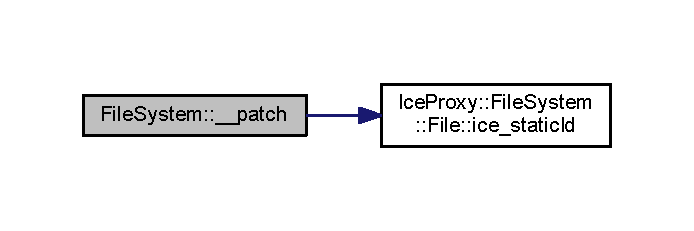
\includegraphics[width=333pt]{namespace_file_system_a51d618729b59cf8ad7823ff14af488de_cgraph}
\end{center}
\end{figure}


\hypertarget{namespace_file_system_a9c85bcf49db4963463099447f95e0dab}{}\index{File\+System@{File\+System}!new\+Callback\+\_\+\+File\+\_\+get\+History@{new\+Callback\+\_\+\+File\+\_\+get\+History}}
\index{new\+Callback\+\_\+\+File\+\_\+get\+History@{new\+Callback\+\_\+\+File\+\_\+get\+History}!File\+System@{File\+System}}
\subsubsection[{new\+Callback\+\_\+\+File\+\_\+get\+History}]{\setlength{\rightskip}{0pt plus 5cm}template$<$class T $>$ {\bf Callback\+\_\+\+File\+\_\+get\+History\+Ptr} File\+System\+::new\+Callback\+\_\+\+File\+\_\+get\+History (
\begin{DoxyParamCaption}
\item[{const Ice\+Util\+::\+Handle$<$ T $>$ \&}]{instance, }
\item[{void(T\+::$\ast$)(const \+::{\bf File\+System\+::\+Ver\+Seq} \&)}]{cb, }
\item[{void(T\+::$\ast$)(const \+::Ice\+::\+Exception \&)}]{excb, }
\item[{void(T\+::$\ast$)(bool)}]{sentcb = {\ttfamily 0}}
\end{DoxyParamCaption}
)}\label{namespace_file_system_a9c85bcf49db4963463099447f95e0dab}
\hypertarget{namespace_file_system_ad5d2a7211c35dfd59a100b8672b42fae}{}\index{File\+System@{File\+System}!new\+Callback\+\_\+\+File\+\_\+get\+History@{new\+Callback\+\_\+\+File\+\_\+get\+History}}
\index{new\+Callback\+\_\+\+File\+\_\+get\+History@{new\+Callback\+\_\+\+File\+\_\+get\+History}!File\+System@{File\+System}}
\subsubsection[{new\+Callback\+\_\+\+File\+\_\+get\+History}]{\setlength{\rightskip}{0pt plus 5cm}template$<$class T $>$ {\bf Callback\+\_\+\+File\+\_\+get\+History\+Ptr} File\+System\+::new\+Callback\+\_\+\+File\+\_\+get\+History (
\begin{DoxyParamCaption}
\item[{T $\ast$}]{instance, }
\item[{void(T\+::$\ast$)(const \+::{\bf File\+System\+::\+Ver\+Seq} \&)}]{cb, }
\item[{void(T\+::$\ast$)(const \+::Ice\+::\+Exception \&)}]{excb, }
\item[{void(T\+::$\ast$)(bool)}]{sentcb = {\ttfamily 0}}
\end{DoxyParamCaption}
)}\label{namespace_file_system_ad5d2a7211c35dfd59a100b8672b42fae}
\hypertarget{namespace_file_system_a452d710fbcda80656c790b9c5fd63518}{}\index{File\+System@{File\+System}!new\+Callback\+\_\+\+File\+\_\+get\+History@{new\+Callback\+\_\+\+File\+\_\+get\+History}}
\index{new\+Callback\+\_\+\+File\+\_\+get\+History@{new\+Callback\+\_\+\+File\+\_\+get\+History}!File\+System@{File\+System}}
\subsubsection[{new\+Callback\+\_\+\+File\+\_\+get\+History}]{\setlength{\rightskip}{0pt plus 5cm}template$<$class T , typename C\+T $>$ {\bf Callback\+\_\+\+File\+\_\+get\+History\+Ptr} File\+System\+::new\+Callback\+\_\+\+File\+\_\+get\+History (
\begin{DoxyParamCaption}
\item[{const Ice\+Util\+::\+Handle$<$ T $>$ \&}]{instance, }
\item[{void(T\+::$\ast$)(const \+::{\bf File\+System\+::\+Ver\+Seq} \&, const C\+T \&)}]{cb, }
\item[{void(T\+::$\ast$)(const \+::Ice\+::\+Exception \&, const C\+T \&)}]{excb, }
\item[{void(T\+::$\ast$)(bool, const C\+T \&)}]{sentcb = {\ttfamily 0}}
\end{DoxyParamCaption}
)}\label{namespace_file_system_a452d710fbcda80656c790b9c5fd63518}
\hypertarget{namespace_file_system_acaebd2ccc7b6507ce9791aa62af99829}{}\index{File\+System@{File\+System}!new\+Callback\+\_\+\+File\+\_\+get\+History@{new\+Callback\+\_\+\+File\+\_\+get\+History}}
\index{new\+Callback\+\_\+\+File\+\_\+get\+History@{new\+Callback\+\_\+\+File\+\_\+get\+History}!File\+System@{File\+System}}
\subsubsection[{new\+Callback\+\_\+\+File\+\_\+get\+History}]{\setlength{\rightskip}{0pt plus 5cm}template$<$class T , typename C\+T $>$ {\bf Callback\+\_\+\+File\+\_\+get\+History\+Ptr} File\+System\+::new\+Callback\+\_\+\+File\+\_\+get\+History (
\begin{DoxyParamCaption}
\item[{T $\ast$}]{instance, }
\item[{void(T\+::$\ast$)(const \+::{\bf File\+System\+::\+Ver\+Seq} \&, const C\+T \&)}]{cb, }
\item[{void(T\+::$\ast$)(const \+::Ice\+::\+Exception \&, const C\+T \&)}]{excb, }
\item[{void(T\+::$\ast$)(bool, const C\+T \&)}]{sentcb = {\ttfamily 0}}
\end{DoxyParamCaption}
)}\label{namespace_file_system_acaebd2ccc7b6507ce9791aa62af99829}
\hypertarget{namespace_file_system_a8cc04448ea3637125a33672fbd8f01db}{}\index{File\+System@{File\+System}!new\+Callback\+\_\+\+File\+\_\+receive\+Latest@{new\+Callback\+\_\+\+File\+\_\+receive\+Latest}}
\index{new\+Callback\+\_\+\+File\+\_\+receive\+Latest@{new\+Callback\+\_\+\+File\+\_\+receive\+Latest}!File\+System@{File\+System}}
\subsubsection[{new\+Callback\+\_\+\+File\+\_\+receive\+Latest}]{\setlength{\rightskip}{0pt plus 5cm}template$<$class T $>$ {\bf Callback\+\_\+\+File\+\_\+receive\+Latest\+Ptr} File\+System\+::new\+Callback\+\_\+\+File\+\_\+receive\+Latest (
\begin{DoxyParamCaption}
\item[{const Ice\+Util\+::\+Handle$<$ T $>$ \&}]{instance, }
\item[{void(T\+::$\ast$)(const \+::{\bf File\+System\+::\+Byte\+Seq} \&)}]{cb, }
\item[{void(T\+::$\ast$)(const \+::Ice\+::\+Exception \&)}]{excb, }
\item[{void(T\+::$\ast$)(bool)}]{sentcb = {\ttfamily 0}}
\end{DoxyParamCaption}
)}\label{namespace_file_system_a8cc04448ea3637125a33672fbd8f01db}
\hypertarget{namespace_file_system_a4fbffcbd3a07944195f823e591bb353d}{}\index{File\+System@{File\+System}!new\+Callback\+\_\+\+File\+\_\+receive\+Latest@{new\+Callback\+\_\+\+File\+\_\+receive\+Latest}}
\index{new\+Callback\+\_\+\+File\+\_\+receive\+Latest@{new\+Callback\+\_\+\+File\+\_\+receive\+Latest}!File\+System@{File\+System}}
\subsubsection[{new\+Callback\+\_\+\+File\+\_\+receive\+Latest}]{\setlength{\rightskip}{0pt plus 5cm}template$<$class T $>$ {\bf Callback\+\_\+\+File\+\_\+receive\+Latest\+Ptr} File\+System\+::new\+Callback\+\_\+\+File\+\_\+receive\+Latest (
\begin{DoxyParamCaption}
\item[{T $\ast$}]{instance, }
\item[{void(T\+::$\ast$)(const \+::{\bf File\+System\+::\+Byte\+Seq} \&)}]{cb, }
\item[{void(T\+::$\ast$)(const \+::Ice\+::\+Exception \&)}]{excb, }
\item[{void(T\+::$\ast$)(bool)}]{sentcb = {\ttfamily 0}}
\end{DoxyParamCaption}
)}\label{namespace_file_system_a4fbffcbd3a07944195f823e591bb353d}
\hypertarget{namespace_file_system_a0046b7a52a5238cb4aec849e4ccd3f15}{}\index{File\+System@{File\+System}!new\+Callback\+\_\+\+File\+\_\+receive\+Latest@{new\+Callback\+\_\+\+File\+\_\+receive\+Latest}}
\index{new\+Callback\+\_\+\+File\+\_\+receive\+Latest@{new\+Callback\+\_\+\+File\+\_\+receive\+Latest}!File\+System@{File\+System}}
\subsubsection[{new\+Callback\+\_\+\+File\+\_\+receive\+Latest}]{\setlength{\rightskip}{0pt plus 5cm}template$<$class T , typename C\+T $>$ {\bf Callback\+\_\+\+File\+\_\+receive\+Latest\+Ptr} File\+System\+::new\+Callback\+\_\+\+File\+\_\+receive\+Latest (
\begin{DoxyParamCaption}
\item[{const Ice\+Util\+::\+Handle$<$ T $>$ \&}]{instance, }
\item[{void(T\+::$\ast$)(const \+::{\bf File\+System\+::\+Byte\+Seq} \&, const C\+T \&)}]{cb, }
\item[{void(T\+::$\ast$)(const \+::Ice\+::\+Exception \&, const C\+T \&)}]{excb, }
\item[{void(T\+::$\ast$)(bool, const C\+T \&)}]{sentcb = {\ttfamily 0}}
\end{DoxyParamCaption}
)}\label{namespace_file_system_a0046b7a52a5238cb4aec849e4ccd3f15}
\hypertarget{namespace_file_system_ab3edd75e3503f455de67f53659888e54}{}\index{File\+System@{File\+System}!new\+Callback\+\_\+\+File\+\_\+receive\+Latest@{new\+Callback\+\_\+\+File\+\_\+receive\+Latest}}
\index{new\+Callback\+\_\+\+File\+\_\+receive\+Latest@{new\+Callback\+\_\+\+File\+\_\+receive\+Latest}!File\+System@{File\+System}}
\subsubsection[{new\+Callback\+\_\+\+File\+\_\+receive\+Latest}]{\setlength{\rightskip}{0pt plus 5cm}template$<$class T , typename C\+T $>$ {\bf Callback\+\_\+\+File\+\_\+receive\+Latest\+Ptr} File\+System\+::new\+Callback\+\_\+\+File\+\_\+receive\+Latest (
\begin{DoxyParamCaption}
\item[{T $\ast$}]{instance, }
\item[{void(T\+::$\ast$)(const \+::{\bf File\+System\+::\+Byte\+Seq} \&, const C\+T \&)}]{cb, }
\item[{void(T\+::$\ast$)(const \+::Ice\+::\+Exception \&, const C\+T \&)}]{excb, }
\item[{void(T\+::$\ast$)(bool, const C\+T \&)}]{sentcb = {\ttfamily 0}}
\end{DoxyParamCaption}
)}\label{namespace_file_system_ab3edd75e3503f455de67f53659888e54}
\hypertarget{namespace_file_system_a42d5739a2f8c21dd11147976f3899b6a}{}\index{File\+System@{File\+System}!new\+Callback\+\_\+\+File\+\_\+receive\+Version@{new\+Callback\+\_\+\+File\+\_\+receive\+Version}}
\index{new\+Callback\+\_\+\+File\+\_\+receive\+Version@{new\+Callback\+\_\+\+File\+\_\+receive\+Version}!File\+System@{File\+System}}
\subsubsection[{new\+Callback\+\_\+\+File\+\_\+receive\+Version}]{\setlength{\rightskip}{0pt plus 5cm}template$<$class T $>$ {\bf Callback\+\_\+\+File\+\_\+receive\+Version\+Ptr} File\+System\+::new\+Callback\+\_\+\+File\+\_\+receive\+Version (
\begin{DoxyParamCaption}
\item[{const Ice\+Util\+::\+Handle$<$ T $>$ \&}]{instance, }
\item[{void(T\+::$\ast$)(const \+::{\bf File\+System\+::\+Byte\+Seq} \&)}]{cb, }
\item[{void(T\+::$\ast$)(const \+::Ice\+::\+Exception \&)}]{excb, }
\item[{void(T\+::$\ast$)(bool)}]{sentcb = {\ttfamily 0}}
\end{DoxyParamCaption}
)}\label{namespace_file_system_a42d5739a2f8c21dd11147976f3899b6a}
\hypertarget{namespace_file_system_a03da11fc8fef703e71e714806a453d0f}{}\index{File\+System@{File\+System}!new\+Callback\+\_\+\+File\+\_\+receive\+Version@{new\+Callback\+\_\+\+File\+\_\+receive\+Version}}
\index{new\+Callback\+\_\+\+File\+\_\+receive\+Version@{new\+Callback\+\_\+\+File\+\_\+receive\+Version}!File\+System@{File\+System}}
\subsubsection[{new\+Callback\+\_\+\+File\+\_\+receive\+Version}]{\setlength{\rightskip}{0pt plus 5cm}template$<$class T $>$ {\bf Callback\+\_\+\+File\+\_\+receive\+Version\+Ptr} File\+System\+::new\+Callback\+\_\+\+File\+\_\+receive\+Version (
\begin{DoxyParamCaption}
\item[{T $\ast$}]{instance, }
\item[{void(T\+::$\ast$)(const \+::{\bf File\+System\+::\+Byte\+Seq} \&)}]{cb, }
\item[{void(T\+::$\ast$)(const \+::Ice\+::\+Exception \&)}]{excb, }
\item[{void(T\+::$\ast$)(bool)}]{sentcb = {\ttfamily 0}}
\end{DoxyParamCaption}
)}\label{namespace_file_system_a03da11fc8fef703e71e714806a453d0f}
\hypertarget{namespace_file_system_aca4582991eb93cb8a1826c2387679604}{}\index{File\+System@{File\+System}!new\+Callback\+\_\+\+File\+\_\+receive\+Version@{new\+Callback\+\_\+\+File\+\_\+receive\+Version}}
\index{new\+Callback\+\_\+\+File\+\_\+receive\+Version@{new\+Callback\+\_\+\+File\+\_\+receive\+Version}!File\+System@{File\+System}}
\subsubsection[{new\+Callback\+\_\+\+File\+\_\+receive\+Version}]{\setlength{\rightskip}{0pt plus 5cm}template$<$class T , typename C\+T $>$ {\bf Callback\+\_\+\+File\+\_\+receive\+Version\+Ptr} File\+System\+::new\+Callback\+\_\+\+File\+\_\+receive\+Version (
\begin{DoxyParamCaption}
\item[{const Ice\+Util\+::\+Handle$<$ T $>$ \&}]{instance, }
\item[{void(T\+::$\ast$)(const \+::{\bf File\+System\+::\+Byte\+Seq} \&, const C\+T \&)}]{cb, }
\item[{void(T\+::$\ast$)(const \+::Ice\+::\+Exception \&, const C\+T \&)}]{excb, }
\item[{void(T\+::$\ast$)(bool, const C\+T \&)}]{sentcb = {\ttfamily 0}}
\end{DoxyParamCaption}
)}\label{namespace_file_system_aca4582991eb93cb8a1826c2387679604}
\hypertarget{namespace_file_system_adf4cdf405caaf42582f7d55bf48d5702}{}\index{File\+System@{File\+System}!new\+Callback\+\_\+\+File\+\_\+receive\+Version@{new\+Callback\+\_\+\+File\+\_\+receive\+Version}}
\index{new\+Callback\+\_\+\+File\+\_\+receive\+Version@{new\+Callback\+\_\+\+File\+\_\+receive\+Version}!File\+System@{File\+System}}
\subsubsection[{new\+Callback\+\_\+\+File\+\_\+receive\+Version}]{\setlength{\rightskip}{0pt plus 5cm}template$<$class T , typename C\+T $>$ {\bf Callback\+\_\+\+File\+\_\+receive\+Version\+Ptr} File\+System\+::new\+Callback\+\_\+\+File\+\_\+receive\+Version (
\begin{DoxyParamCaption}
\item[{T $\ast$}]{instance, }
\item[{void(T\+::$\ast$)(const \+::{\bf File\+System\+::\+Byte\+Seq} \&, const C\+T \&)}]{cb, }
\item[{void(T\+::$\ast$)(const \+::Ice\+::\+Exception \&, const C\+T \&)}]{excb, }
\item[{void(T\+::$\ast$)(bool, const C\+T \&)}]{sentcb = {\ttfamily 0}}
\end{DoxyParamCaption}
)}\label{namespace_file_system_adf4cdf405caaf42582f7d55bf48d5702}
\hypertarget{namespace_file_system_a19a234cedd70c1fd80bb5f5c842c3041}{}\index{File\+System@{File\+System}!new\+Callback\+\_\+\+File\+\_\+send\+File@{new\+Callback\+\_\+\+File\+\_\+send\+File}}
\index{new\+Callback\+\_\+\+File\+\_\+send\+File@{new\+Callback\+\_\+\+File\+\_\+send\+File}!File\+System@{File\+System}}
\subsubsection[{new\+Callback\+\_\+\+File\+\_\+send\+File}]{\setlength{\rightskip}{0pt plus 5cm}template$<$class T $>$ {\bf Callback\+\_\+\+File\+\_\+send\+File\+Ptr} File\+System\+::new\+Callback\+\_\+\+File\+\_\+send\+File (
\begin{DoxyParamCaption}
\item[{const Ice\+Util\+::\+Handle$<$ T $>$ \&}]{instance, }
\item[{void(T\+::$\ast$)(bool)}]{cb, }
\item[{void(T\+::$\ast$)(const \+::Ice\+::\+Exception \&)}]{excb, }
\item[{void(T\+::$\ast$)(bool)}]{sentcb = {\ttfamily 0}}
\end{DoxyParamCaption}
)}\label{namespace_file_system_a19a234cedd70c1fd80bb5f5c842c3041}
\hypertarget{namespace_file_system_a940c86675dd438dacf7618250756a3c0}{}\index{File\+System@{File\+System}!new\+Callback\+\_\+\+File\+\_\+send\+File@{new\+Callback\+\_\+\+File\+\_\+send\+File}}
\index{new\+Callback\+\_\+\+File\+\_\+send\+File@{new\+Callback\+\_\+\+File\+\_\+send\+File}!File\+System@{File\+System}}
\subsubsection[{new\+Callback\+\_\+\+File\+\_\+send\+File}]{\setlength{\rightskip}{0pt plus 5cm}template$<$class T $>$ {\bf Callback\+\_\+\+File\+\_\+send\+File\+Ptr} File\+System\+::new\+Callback\+\_\+\+File\+\_\+send\+File (
\begin{DoxyParamCaption}
\item[{T $\ast$}]{instance, }
\item[{void(T\+::$\ast$)(bool)}]{cb, }
\item[{void(T\+::$\ast$)(const \+::Ice\+::\+Exception \&)}]{excb, }
\item[{void(T\+::$\ast$)(bool)}]{sentcb = {\ttfamily 0}}
\end{DoxyParamCaption}
)}\label{namespace_file_system_a940c86675dd438dacf7618250756a3c0}
\hypertarget{namespace_file_system_a018b94a8e4bb414a2eb5b880dfd2309d}{}\index{File\+System@{File\+System}!new\+Callback\+\_\+\+File\+\_\+send\+File@{new\+Callback\+\_\+\+File\+\_\+send\+File}}
\index{new\+Callback\+\_\+\+File\+\_\+send\+File@{new\+Callback\+\_\+\+File\+\_\+send\+File}!File\+System@{File\+System}}
\subsubsection[{new\+Callback\+\_\+\+File\+\_\+send\+File}]{\setlength{\rightskip}{0pt plus 5cm}template$<$class T , typename C\+T $>$ {\bf Callback\+\_\+\+File\+\_\+send\+File\+Ptr} File\+System\+::new\+Callback\+\_\+\+File\+\_\+send\+File (
\begin{DoxyParamCaption}
\item[{const Ice\+Util\+::\+Handle$<$ T $>$ \&}]{instance, }
\item[{void(T\+::$\ast$)(bool, const C\+T \&)}]{cb, }
\item[{void(T\+::$\ast$)(const \+::Ice\+::\+Exception \&, const C\+T \&)}]{excb, }
\item[{void(T\+::$\ast$)(bool, const C\+T \&)}]{sentcb = {\ttfamily 0}}
\end{DoxyParamCaption}
)}\label{namespace_file_system_a018b94a8e4bb414a2eb5b880dfd2309d}
\hypertarget{namespace_file_system_a617605b6d0e9224ad5d7d424600651da}{}\index{File\+System@{File\+System}!new\+Callback\+\_\+\+File\+\_\+send\+File@{new\+Callback\+\_\+\+File\+\_\+send\+File}}
\index{new\+Callback\+\_\+\+File\+\_\+send\+File@{new\+Callback\+\_\+\+File\+\_\+send\+File}!File\+System@{File\+System}}
\subsubsection[{new\+Callback\+\_\+\+File\+\_\+send\+File}]{\setlength{\rightskip}{0pt plus 5cm}template$<$class T , typename C\+T $>$ {\bf Callback\+\_\+\+File\+\_\+send\+File\+Ptr} File\+System\+::new\+Callback\+\_\+\+File\+\_\+send\+File (
\begin{DoxyParamCaption}
\item[{T $\ast$}]{instance, }
\item[{void(T\+::$\ast$)(bool, const C\+T \&)}]{cb, }
\item[{void(T\+::$\ast$)(const \+::Ice\+::\+Exception \&, const C\+T \&)}]{excb, }
\item[{void(T\+::$\ast$)(bool, const C\+T \&)}]{sentcb = {\ttfamily 0}}
\end{DoxyParamCaption}
)}\label{namespace_file_system_a617605b6d0e9224ad5d7d424600651da}
\hypertarget{namespace_file_system_ace2c44fa41a64ff7b2d5262d77563c06}{}\index{File\+System@{File\+System}!operator$<$@{operator$<$}}
\index{operator$<$@{operator$<$}!File\+System@{File\+System}}
\subsubsection[{operator$<$}]{\setlength{\rightskip}{0pt plus 5cm}bool File\+System\+::operator$<$ (
\begin{DoxyParamCaption}
\item[{const {\bf File} \&}]{l, }
\item[{const {\bf File} \&}]{r}
\end{DoxyParamCaption}
)\hspace{0.3cm}{\ttfamily [inline]}}\label{namespace_file_system_ace2c44fa41a64ff7b2d5262d77563c06}
\hypertarget{namespace_file_system_a73ba38c87f762f68818866f670cdece9}{}\index{File\+System@{File\+System}!operator==@{operator==}}
\index{operator==@{operator==}!File\+System@{File\+System}}
\subsubsection[{operator==}]{\setlength{\rightskip}{0pt plus 5cm}bool File\+System\+::operator== (
\begin{DoxyParamCaption}
\item[{const {\bf File} \&}]{l, }
\item[{const {\bf File} \&}]{r}
\end{DoxyParamCaption}
)\hspace{0.3cm}{\ttfamily [inline]}}\label{namespace_file_system_a73ba38c87f762f68818866f670cdece9}
\hypertarget{namespace_file_system_a918f916e3b881056468148cf34e98734}{}\index{File\+System@{File\+System}!up\+Cast@{up\+Cast}}
\index{up\+Cast@{up\+Cast}!File\+System@{File\+System}}
\subsubsection[{up\+Cast}]{\setlength{\rightskip}{0pt plus 5cm}Ice\+::\+Object $\ast$ File\+System\+::up\+Cast (
\begin{DoxyParamCaption}
\item[{\+::{\bf File\+System\+::\+File} $\ast$}]{p}
\end{DoxyParamCaption}
)}\label{namespace_file_system_a918f916e3b881056468148cf34e98734}

\hypertarget{namespace_ice}{}\section{Ice Namespace Reference}
\label{namespace_ice}\index{Ice@{Ice}}
\subsection*{Classes}
\begin{DoxyCompactItemize}
\item 
struct \hyperlink{struct_ice_1_1_streamable_traits_3_01_1_1_file_system_1_1_version_01_4}{Streamable\+Traits$<$ \+::\+File\+System\+::\+Version $>$}
\item 
struct \hyperlink{struct_ice_1_1_stream_reader_3_01_1_1_file_system_1_1_version_00_01_s_01_4}{Stream\+Reader$<$ \+::\+File\+System\+::\+Version, S $>$}
\item 
struct \hyperlink{struct_ice_1_1_stream_writer_3_01_1_1_file_system_1_1_version_00_01_s_01_4}{Stream\+Writer$<$ \+::\+File\+System\+::\+Version, S $>$}
\end{DoxyCompactItemize}

\hypertarget{namespace_ice_delegate}{}\section{Ice\+Delegate Namespace Reference}
\label{namespace_ice_delegate}\index{Ice\+Delegate@{Ice\+Delegate}}
\subsection*{Namespaces}
\begin{DoxyCompactItemize}
\item 
 \hyperlink{namespace_ice_delegate_1_1_file_system}{File\+System}
\end{DoxyCompactItemize}

\hypertarget{namespace_ice_delegate_1_1_file_system}{}\section{Ice\+Delegate\+:\+:File\+System Namespace Reference}
\label{namespace_ice_delegate_1_1_file_system}\index{Ice\+Delegate\+::\+File\+System@{Ice\+Delegate\+::\+File\+System}}
\subsection*{Classes}
\begin{DoxyCompactItemize}
\item 
class \hyperlink{class_ice_delegate_1_1_file_system_1_1_file}{File}
\end{DoxyCompactItemize}

\hypertarget{namespace_ice_delegate_d}{}\section{Ice\+Delegate\+D Namespace Reference}
\label{namespace_ice_delegate_d}\index{Ice\+Delegate\+D@{Ice\+Delegate\+D}}
\subsection*{Namespaces}
\begin{DoxyCompactItemize}
\item 
 \hyperlink{namespace_ice_delegate_d_1_1_file_system}{File\+System}
\end{DoxyCompactItemize}

\hypertarget{namespace_ice_delegate_d_1_1_file_system}{}\section{Ice\+Delegate\+D\+:\+:File\+System Namespace Reference}
\label{namespace_ice_delegate_d_1_1_file_system}\index{Ice\+Delegate\+D\+::\+File\+System@{Ice\+Delegate\+D\+::\+File\+System}}
\subsection*{Classes}
\begin{DoxyCompactItemize}
\item 
class \hyperlink{class_ice_delegate_d_1_1_file_system_1_1_file}{File}
\end{DoxyCompactItemize}

\hypertarget{namespace_ice_delegate_m}{}\section{Ice\+Delegate\+M Namespace Reference}
\label{namespace_ice_delegate_m}\index{Ice\+Delegate\+M@{Ice\+Delegate\+M}}
\subsection*{Namespaces}
\begin{DoxyCompactItemize}
\item 
 \hyperlink{namespace_ice_delegate_m_1_1_file_system}{File\+System}
\end{DoxyCompactItemize}

\hypertarget{namespace_ice_delegate_m_1_1_file_system}{}\section{Ice\+Delegate\+M\+:\+:File\+System Namespace Reference}
\label{namespace_ice_delegate_m_1_1_file_system}\index{Ice\+Delegate\+M\+::\+File\+System@{Ice\+Delegate\+M\+::\+File\+System}}
\subsection*{Classes}
\begin{DoxyCompactItemize}
\item 
class \hyperlink{class_ice_delegate_m_1_1_file_system_1_1_file}{File}
\end{DoxyCompactItemize}

\hypertarget{namespace_ice_proxy}{}\section{Ice\+Proxy Namespace Reference}
\label{namespace_ice_proxy}\index{Ice\+Proxy@{Ice\+Proxy}}
\subsection*{Namespaces}
\begin{DoxyCompactItemize}
\item 
 \hyperlink{namespace_ice_proxy_1_1_file_system}{File\+System}
\end{DoxyCompactItemize}

\hypertarget{namespace_ice_proxy_1_1_file_system}{}\section{Ice\+Proxy\+:\+:File\+System Namespace Reference}
\label{namespace_ice_proxy_1_1_file_system}\index{Ice\+Proxy\+::\+File\+System@{Ice\+Proxy\+::\+File\+System}}
\subsection*{Classes}
\begin{DoxyCompactItemize}
\item 
class \hyperlink{class_ice_proxy_1_1_file_system_1_1_file}{File}
\end{DoxyCompactItemize}
\subsection*{Functions}
\begin{DoxyCompactItemize}
\item 
void \hyperlink{namespace_ice_proxy_1_1_file_system_a0b249e87c3baee8b137cf42677c53635}{\+\_\+\+\_\+read} (\+::Ice\+Internal\+::\+Basic\+Stream $\ast$,\+::Ice\+Internal\+::\+Proxy\+Handle$<$ \+::\hyperlink{class_ice_proxy_1_1_file_system_1_1_file}{Ice\+Proxy\+::\+File\+System\+::\+File} $>$ \&)
\item 
\+::Ice\+Proxy\+::\+Ice\+::\+Object $\ast$ \hyperlink{namespace_ice_proxy_1_1_file_system_acb20dd4ca34a1045e77c7e64f5faa83a}{up\+Cast} (\+::\hyperlink{class_ice_proxy_1_1_file_system_1_1_file}{Ice\+Proxy\+::\+File\+System\+::\+File} $\ast$)
\end{DoxyCompactItemize}


\subsection{Function Documentation}
\hypertarget{namespace_ice_proxy_1_1_file_system_a0b249e87c3baee8b137cf42677c53635}{}\index{Ice\+Proxy\+::\+File\+System@{Ice\+Proxy\+::\+File\+System}!\+\_\+\+\_\+read@{\+\_\+\+\_\+read}}
\index{\+\_\+\+\_\+read@{\+\_\+\+\_\+read}!Ice\+Proxy\+::\+File\+System@{Ice\+Proxy\+::\+File\+System}}
\subsubsection[{\+\_\+\+\_\+read}]{\setlength{\rightskip}{0pt plus 5cm}void Ice\+Proxy\+::\+File\+System\+::\+\_\+\+\_\+read (
\begin{DoxyParamCaption}
\item[{\+::Ice\+Internal\+::\+Basic\+Stream $\ast$}]{, }
\item[{\+::Ice\+Internal\+::\+Proxy\+Handle$<$ \+::{\bf Ice\+Proxy\+::\+File\+System\+::\+File} $>$ \&}]{}
\end{DoxyParamCaption}
)}\label{namespace_ice_proxy_1_1_file_system_a0b249e87c3baee8b137cf42677c53635}
\hypertarget{namespace_ice_proxy_1_1_file_system_acb20dd4ca34a1045e77c7e64f5faa83a}{}\index{Ice\+Proxy\+::\+File\+System@{Ice\+Proxy\+::\+File\+System}!up\+Cast@{up\+Cast}}
\index{up\+Cast@{up\+Cast}!Ice\+Proxy\+::\+File\+System@{Ice\+Proxy\+::\+File\+System}}
\subsubsection[{up\+Cast}]{\setlength{\rightskip}{0pt plus 5cm}Ice\+Proxy\+::\+Ice\+::\+Object $\ast$ Ice\+Proxy\+::\+File\+System\+::up\+Cast (
\begin{DoxyParamCaption}
\item[{\+::{\bf Ice\+Proxy\+::\+File\+System\+::\+File} $\ast$}]{p}
\end{DoxyParamCaption}
)}\label{namespace_ice_proxy_1_1_file_system_acb20dd4ca34a1045e77c7e64f5faa83a}

\chapter{Class Documentation}
\hypertarget{class_file_system_1_1_callback___file__get_history}{}\section{File\+System\+:\+:Callback\+\_\+\+File\+\_\+get\+History$<$ T, C\+T $>$ Class Template Reference}
\label{class_file_system_1_1_callback___file__get_history}\index{File\+System\+::\+Callback\+\_\+\+File\+\_\+get\+History$<$ T, C\+T $>$@{File\+System\+::\+Callback\+\_\+\+File\+\_\+get\+History$<$ T, C\+T $>$}}


{\ttfamily \#include $<$File\+System.\+h$>$}



Inheritance diagram for File\+System\+:\+:Callback\+\_\+\+File\+\_\+get\+History$<$ T, C\+T $>$\+:
\nopagebreak
\begin{figure}[H]
\begin{center}
\leavevmode
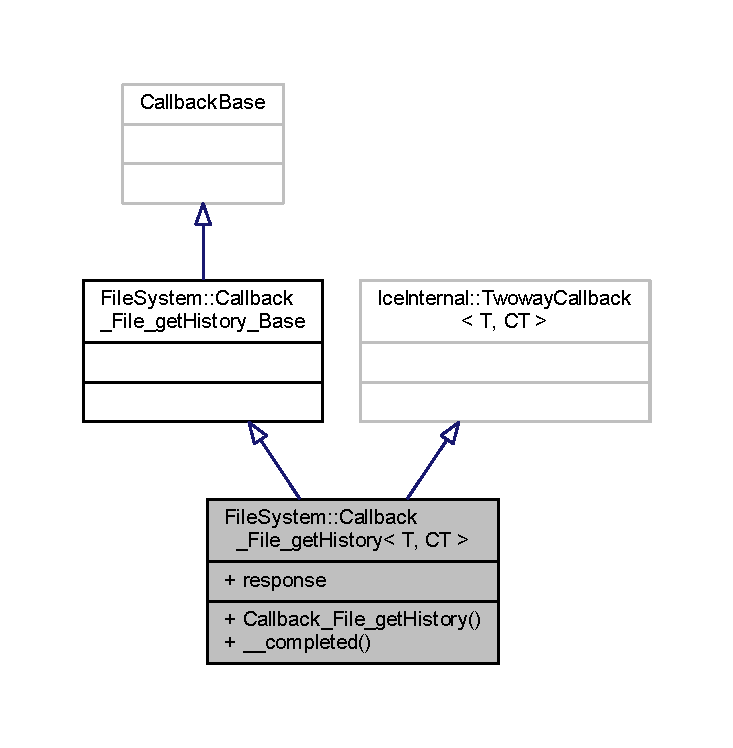
\includegraphics[width=350pt]{class_file_system_1_1_callback___file__get_history__inherit__graph}
\end{center}
\end{figure}


Collaboration diagram for File\+System\+:\+:Callback\+\_\+\+File\+\_\+get\+History$<$ T, C\+T $>$\+:
\nopagebreak
\begin{figure}[H]
\begin{center}
\leavevmode
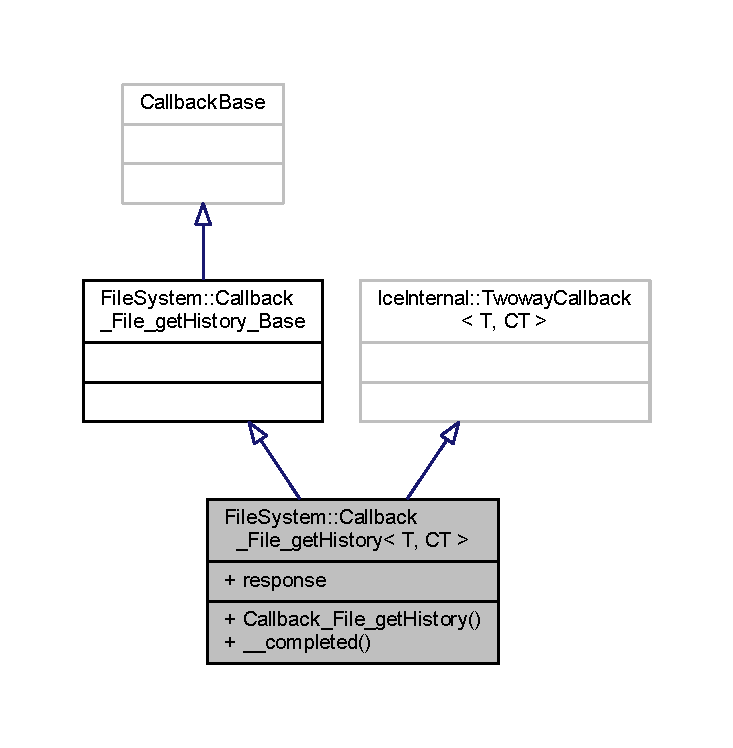
\includegraphics[width=350pt]{class_file_system_1_1_callback___file__get_history__coll__graph}
\end{center}
\end{figure}
\subsection*{Public Types}
\begin{DoxyCompactItemize}
\item 
typedef Ice\+Util\+::\+Handle$<$ T $>$ \hyperlink{class_file_system_1_1_callback___file__get_history_aafd5b2465ab25e9e58402d052d89de42}{T\+Ptr}
\item 
typedef void(T\+::$\ast$ \hyperlink{class_file_system_1_1_callback___file__get_history_a06ee015626144ae9e9b6c7da881698fb}{Exception}) (const \+::Ice\+::\+Exception \&, const C\+T \&)
\item 
typedef void(T\+::$\ast$ \hyperlink{class_file_system_1_1_callback___file__get_history_a9fc8d5d98e242cd24719b4d9727c75cf}{Sent}) (bool, const C\+T \&)
\item 
typedef void(T\+::$\ast$ \hyperlink{class_file_system_1_1_callback___file__get_history_ab5a3b64e414e7c291f6b17ecadecd1db}{Response}) (const \+::\hyperlink{namespace_file_system_ac32dc1eb34c060160b52edc7c4e37d6e}{File\+System\+::\+Ver\+Seq} \&, const C\+T \&)
\end{DoxyCompactItemize}
\subsection*{Public Member Functions}
\begin{DoxyCompactItemize}
\item 
\hyperlink{class_file_system_1_1_callback___file__get_history_a099b4565f686da484102fcbe27eb6a6d}{Callback\+\_\+\+File\+\_\+get\+History} (const \hyperlink{class_file_system_1_1_callback___file__get_history_aafd5b2465ab25e9e58402d052d89de42}{T\+Ptr} \&obj, \hyperlink{class_file_system_1_1_callback___file__get_history_ab5a3b64e414e7c291f6b17ecadecd1db}{Response} cb, \hyperlink{class_file_system_1_1_callback___file__get_history_a06ee015626144ae9e9b6c7da881698fb}{Exception} excb, \hyperlink{class_file_system_1_1_callback___file__get_history_a9fc8d5d98e242cd24719b4d9727c75cf}{Sent} sentcb)
\item 
virtual void \hyperlink{class_file_system_1_1_callback___file__get_history_aca7c379bb2cb7343767aa155cbe47d51}{\+\_\+\+\_\+completed} (const \+::Ice\+::\+Async\+Result\+Ptr \&\+\_\+\+\_\+result) const 
\end{DoxyCompactItemize}
\subsection*{Public Attributes}
\begin{DoxyCompactItemize}
\item 
\hyperlink{class_file_system_1_1_callback___file__get_history_ab5a3b64e414e7c291f6b17ecadecd1db}{Response} \hyperlink{class_file_system_1_1_callback___file__get_history_a16ca6a7305fd1d83892582b167801c6e}{response}
\end{DoxyCompactItemize}


\subsection{Member Typedef Documentation}
\hypertarget{class_file_system_1_1_callback___file__get_history_a06ee015626144ae9e9b6c7da881698fb}{}\index{File\+System\+::\+Callback\+\_\+\+File\+\_\+get\+History@{File\+System\+::\+Callback\+\_\+\+File\+\_\+get\+History}!Exception@{Exception}}
\index{Exception@{Exception}!File\+System\+::\+Callback\+\_\+\+File\+\_\+get\+History@{File\+System\+::\+Callback\+\_\+\+File\+\_\+get\+History}}
\subsubsection[{Exception}]{\setlength{\rightskip}{0pt plus 5cm}template$<$class T, typename C\+T$>$ typedef void(T\+::$\ast$ {\bf File\+System\+::\+Callback\+\_\+\+File\+\_\+get\+History}$<$ T, C\+T $>$\+::Exception) (const \+::Ice\+::\+Exception \&, const C\+T \&)}\label{class_file_system_1_1_callback___file__get_history_a06ee015626144ae9e9b6c7da881698fb}
\hypertarget{class_file_system_1_1_callback___file__get_history_ab5a3b64e414e7c291f6b17ecadecd1db}{}\index{File\+System\+::\+Callback\+\_\+\+File\+\_\+get\+History@{File\+System\+::\+Callback\+\_\+\+File\+\_\+get\+History}!Response@{Response}}
\index{Response@{Response}!File\+System\+::\+Callback\+\_\+\+File\+\_\+get\+History@{File\+System\+::\+Callback\+\_\+\+File\+\_\+get\+History}}
\subsubsection[{Response}]{\setlength{\rightskip}{0pt plus 5cm}template$<$class T, typename C\+T$>$ typedef void(T\+::$\ast$ {\bf File\+System\+::\+Callback\+\_\+\+File\+\_\+get\+History}$<$ T, C\+T $>$\+::Response) (const \+::{\bf File\+System\+::\+Ver\+Seq} \&, const C\+T \&)}\label{class_file_system_1_1_callback___file__get_history_ab5a3b64e414e7c291f6b17ecadecd1db}
\hypertarget{class_file_system_1_1_callback___file__get_history_a9fc8d5d98e242cd24719b4d9727c75cf}{}\index{File\+System\+::\+Callback\+\_\+\+File\+\_\+get\+History@{File\+System\+::\+Callback\+\_\+\+File\+\_\+get\+History}!Sent@{Sent}}
\index{Sent@{Sent}!File\+System\+::\+Callback\+\_\+\+File\+\_\+get\+History@{File\+System\+::\+Callback\+\_\+\+File\+\_\+get\+History}}
\subsubsection[{Sent}]{\setlength{\rightskip}{0pt plus 5cm}template$<$class T, typename C\+T$>$ typedef void(T\+::$\ast$ {\bf File\+System\+::\+Callback\+\_\+\+File\+\_\+get\+History}$<$ T, C\+T $>$\+::Sent) (bool, const C\+T \&)}\label{class_file_system_1_1_callback___file__get_history_a9fc8d5d98e242cd24719b4d9727c75cf}
\hypertarget{class_file_system_1_1_callback___file__get_history_aafd5b2465ab25e9e58402d052d89de42}{}\index{File\+System\+::\+Callback\+\_\+\+File\+\_\+get\+History@{File\+System\+::\+Callback\+\_\+\+File\+\_\+get\+History}!T\+Ptr@{T\+Ptr}}
\index{T\+Ptr@{T\+Ptr}!File\+System\+::\+Callback\+\_\+\+File\+\_\+get\+History@{File\+System\+::\+Callback\+\_\+\+File\+\_\+get\+History}}
\subsubsection[{T\+Ptr}]{\setlength{\rightskip}{0pt plus 5cm}template$<$class T, typename C\+T$>$ typedef Ice\+Util\+::\+Handle$<$T$>$ {\bf File\+System\+::\+Callback\+\_\+\+File\+\_\+get\+History}$<$ T, C\+T $>$\+::{\bf T\+Ptr}}\label{class_file_system_1_1_callback___file__get_history_aafd5b2465ab25e9e58402d052d89de42}


\subsection{Constructor \& Destructor Documentation}
\hypertarget{class_file_system_1_1_callback___file__get_history_a099b4565f686da484102fcbe27eb6a6d}{}\index{File\+System\+::\+Callback\+\_\+\+File\+\_\+get\+History@{File\+System\+::\+Callback\+\_\+\+File\+\_\+get\+History}!Callback\+\_\+\+File\+\_\+get\+History@{Callback\+\_\+\+File\+\_\+get\+History}}
\index{Callback\+\_\+\+File\+\_\+get\+History@{Callback\+\_\+\+File\+\_\+get\+History}!File\+System\+::\+Callback\+\_\+\+File\+\_\+get\+History@{File\+System\+::\+Callback\+\_\+\+File\+\_\+get\+History}}
\subsubsection[{Callback\+\_\+\+File\+\_\+get\+History}]{\setlength{\rightskip}{0pt plus 5cm}template$<$class T, typename C\+T$>$ {\bf File\+System\+::\+Callback\+\_\+\+File\+\_\+get\+History}$<$ T, C\+T $>$\+::{\bf Callback\+\_\+\+File\+\_\+get\+History} (
\begin{DoxyParamCaption}
\item[{const {\bf T\+Ptr} \&}]{obj, }
\item[{{\bf Response}}]{cb, }
\item[{{\bf Exception}}]{excb, }
\item[{{\bf Sent}}]{sentcb}
\end{DoxyParamCaption}
)\hspace{0.3cm}{\ttfamily [inline]}}\label{class_file_system_1_1_callback___file__get_history_a099b4565f686da484102fcbe27eb6a6d}


\subsection{Member Function Documentation}
\hypertarget{class_file_system_1_1_callback___file__get_history_aca7c379bb2cb7343767aa155cbe47d51}{}\index{File\+System\+::\+Callback\+\_\+\+File\+\_\+get\+History@{File\+System\+::\+Callback\+\_\+\+File\+\_\+get\+History}!\+\_\+\+\_\+completed@{\+\_\+\+\_\+completed}}
\index{\+\_\+\+\_\+completed@{\+\_\+\+\_\+completed}!File\+System\+::\+Callback\+\_\+\+File\+\_\+get\+History@{File\+System\+::\+Callback\+\_\+\+File\+\_\+get\+History}}
\subsubsection[{\+\_\+\+\_\+completed}]{\setlength{\rightskip}{0pt plus 5cm}template$<$class T, typename C\+T$>$ virtual void {\bf File\+System\+::\+Callback\+\_\+\+File\+\_\+get\+History}$<$ T, C\+T $>$\+::\+\_\+\+\_\+completed (
\begin{DoxyParamCaption}
\item[{const \+::Ice\+::\+Async\+Result\+Ptr \&}]{\+\_\+\+\_\+result}
\end{DoxyParamCaption}
) const\hspace{0.3cm}{\ttfamily [inline]}, {\ttfamily [virtual]}}\label{class_file_system_1_1_callback___file__get_history_aca7c379bb2cb7343767aa155cbe47d51}


\subsection{Member Data Documentation}
\hypertarget{class_file_system_1_1_callback___file__get_history_a16ca6a7305fd1d83892582b167801c6e}{}\index{File\+System\+::\+Callback\+\_\+\+File\+\_\+get\+History@{File\+System\+::\+Callback\+\_\+\+File\+\_\+get\+History}!response@{response}}
\index{response@{response}!File\+System\+::\+Callback\+\_\+\+File\+\_\+get\+History@{File\+System\+::\+Callback\+\_\+\+File\+\_\+get\+History}}
\subsubsection[{response}]{\setlength{\rightskip}{0pt plus 5cm}template$<$class T, typename C\+T$>$ {\bf Response} {\bf File\+System\+::\+Callback\+\_\+\+File\+\_\+get\+History}$<$ T, C\+T $>$\+::response}\label{class_file_system_1_1_callback___file__get_history_a16ca6a7305fd1d83892582b167801c6e}


The documentation for this class was generated from the following file\+:\begin{DoxyCompactItemize}
\item 
\hyperlink{_file_system_8h}{File\+System.\+h}\end{DoxyCompactItemize}

\hypertarget{class_file_system_1_1_callback___file__get_history___base}{}\section{File\+System\+:\+:Callback\+\_\+\+File\+\_\+get\+History\+\_\+\+Base Class Reference}
\label{class_file_system_1_1_callback___file__get_history___base}\index{File\+System\+::\+Callback\+\_\+\+File\+\_\+get\+History\+\_\+\+Base@{File\+System\+::\+Callback\+\_\+\+File\+\_\+get\+History\+\_\+\+Base}}


{\ttfamily \#include $<$File\+System.\+h$>$}



Inheritance diagram for File\+System\+:\+:Callback\+\_\+\+File\+\_\+get\+History\+\_\+\+Base\+:
\nopagebreak
\begin{figure}[H]
\begin{center}
\leavevmode
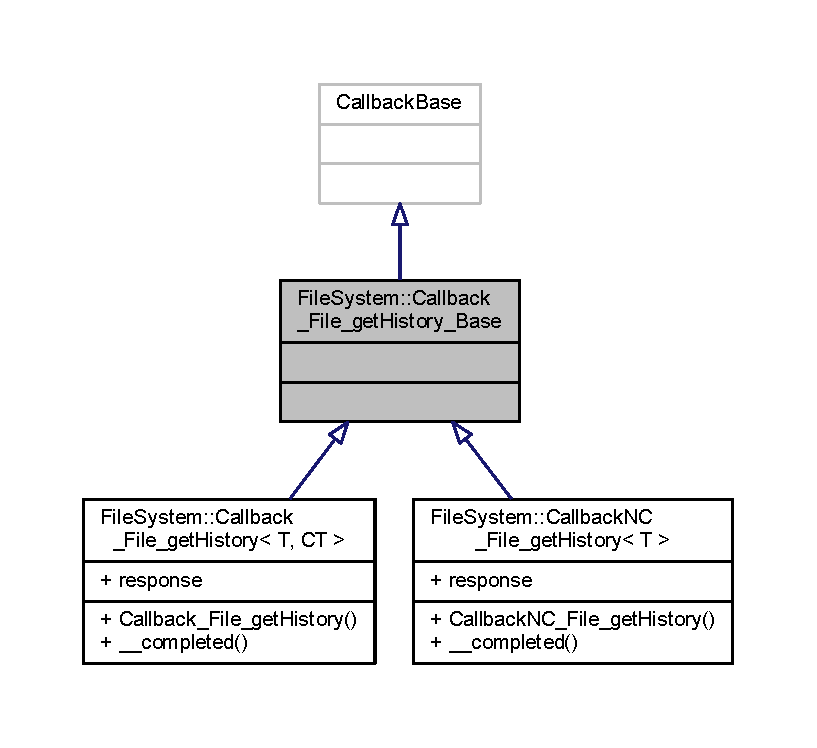
\includegraphics[width=350pt]{class_file_system_1_1_callback___file__get_history___base__inherit__graph}
\end{center}
\end{figure}


Collaboration diagram for File\+System\+:\+:Callback\+\_\+\+File\+\_\+get\+History\+\_\+\+Base\+:
\nopagebreak
\begin{figure}[H]
\begin{center}
\leavevmode
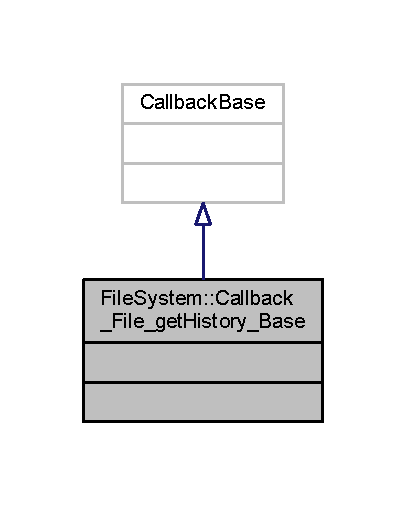
\includegraphics[width=195pt]{class_file_system_1_1_callback___file__get_history___base__coll__graph}
\end{center}
\end{figure}


The documentation for this class was generated from the following file\+:\begin{DoxyCompactItemize}
\item 
\hyperlink{_file_system_8h}{File\+System.\+h}\end{DoxyCompactItemize}

\hypertarget{class_file_system_1_1_callback___file__receive_latest}{}\section{File\+System\+:\+:Callback\+\_\+\+File\+\_\+receive\+Latest$<$ T, C\+T $>$ Class Template Reference}
\label{class_file_system_1_1_callback___file__receive_latest}\index{File\+System\+::\+Callback\+\_\+\+File\+\_\+receive\+Latest$<$ T, C\+T $>$@{File\+System\+::\+Callback\+\_\+\+File\+\_\+receive\+Latest$<$ T, C\+T $>$}}


{\ttfamily \#include $<$File\+System.\+h$>$}



Inheritance diagram for File\+System\+:\+:Callback\+\_\+\+File\+\_\+receive\+Latest$<$ T, C\+T $>$\+:
\nopagebreak
\begin{figure}[H]
\begin{center}
\leavevmode
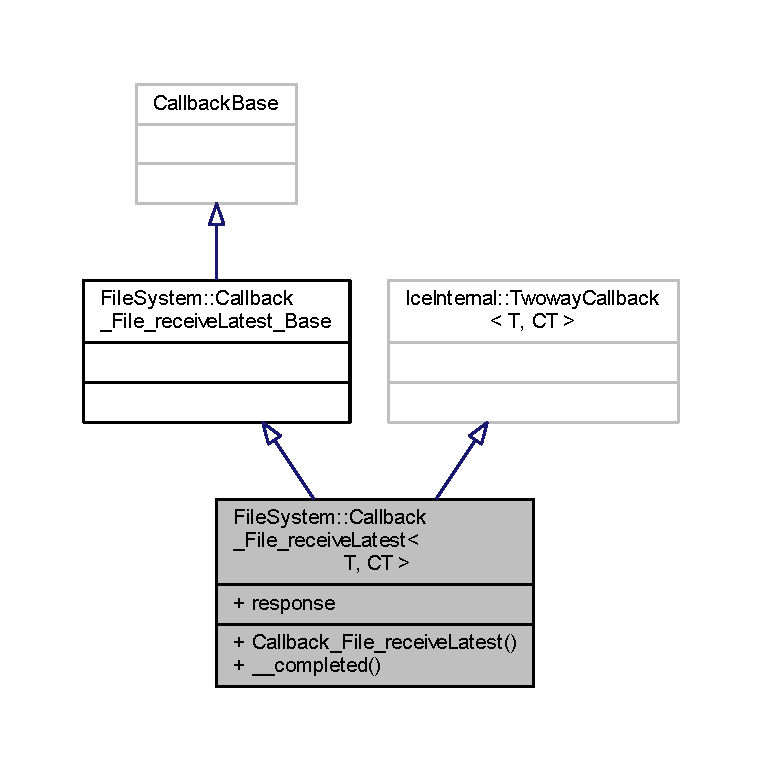
\includegraphics[width=350pt]{class_file_system_1_1_callback___file__receive_latest__inherit__graph}
\end{center}
\end{figure}


Collaboration diagram for File\+System\+:\+:Callback\+\_\+\+File\+\_\+receive\+Latest$<$ T, C\+T $>$\+:
\nopagebreak
\begin{figure}[H]
\begin{center}
\leavevmode
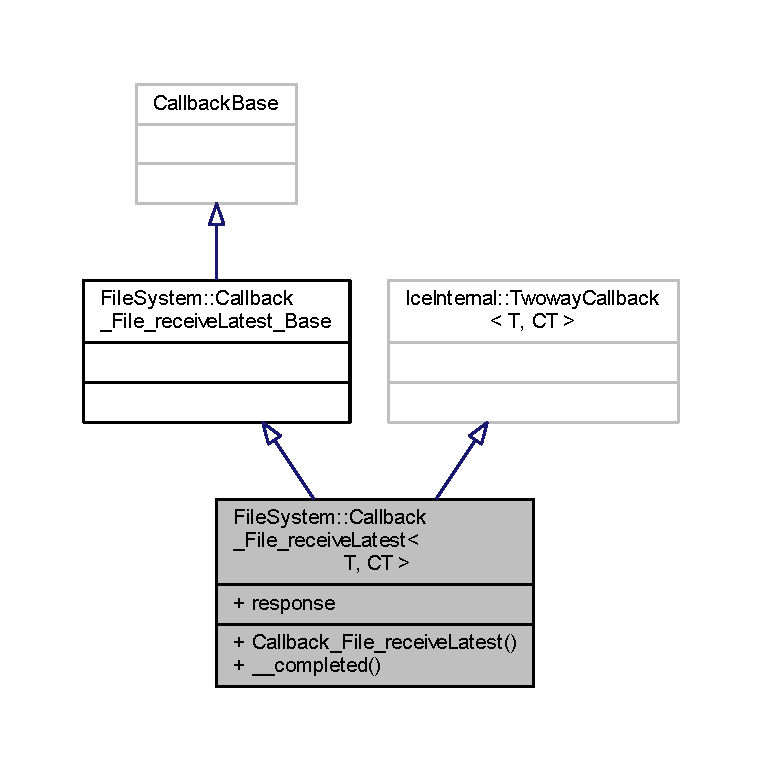
\includegraphics[width=350pt]{class_file_system_1_1_callback___file__receive_latest__coll__graph}
\end{center}
\end{figure}
\subsection*{Public Types}
\begin{DoxyCompactItemize}
\item 
typedef Ice\+Util\+::\+Handle$<$ T $>$ \hyperlink{class_file_system_1_1_callback___file__receive_latest_a8e2064ea01933278c4d3a63cb101d0ce}{T\+Ptr}
\item 
typedef void(T\+::$\ast$ \hyperlink{class_file_system_1_1_callback___file__receive_latest_acc747c11c007fbee3d60c5d85affbe4e}{Exception}) (const \+::Ice\+::\+Exception \&, const C\+T \&)
\item 
typedef void(T\+::$\ast$ \hyperlink{class_file_system_1_1_callback___file__receive_latest_a3a1aaa5cad2e6bb47fd5706274b3afa3}{Sent}) (bool, const C\+T \&)
\item 
typedef void(T\+::$\ast$ \hyperlink{class_file_system_1_1_callback___file__receive_latest_a5bf96c59afd76cc204ef4d42fa6527af}{Response}) (const \+::\hyperlink{namespace_file_system_a5c85de065f9c451ae1d1dea2dacb68c5}{File\+System\+::\+Byte\+Seq} \&, const C\+T \&)
\end{DoxyCompactItemize}
\subsection*{Public Member Functions}
\begin{DoxyCompactItemize}
\item 
\hyperlink{class_file_system_1_1_callback___file__receive_latest_adbf315f6067917f59867ccb1b4257ea8}{Callback\+\_\+\+File\+\_\+receive\+Latest} (const \hyperlink{class_file_system_1_1_callback___file__receive_latest_a8e2064ea01933278c4d3a63cb101d0ce}{T\+Ptr} \&obj, \hyperlink{class_file_system_1_1_callback___file__receive_latest_a5bf96c59afd76cc204ef4d42fa6527af}{Response} cb, \hyperlink{class_file_system_1_1_callback___file__receive_latest_acc747c11c007fbee3d60c5d85affbe4e}{Exception} excb, \hyperlink{class_file_system_1_1_callback___file__receive_latest_a3a1aaa5cad2e6bb47fd5706274b3afa3}{Sent} sentcb)
\item 
virtual void \hyperlink{class_file_system_1_1_callback___file__receive_latest_a266149ea3d3f15cfff0b2130f0b08b52}{\+\_\+\+\_\+completed} (const \+::Ice\+::\+Async\+Result\+Ptr \&\+\_\+\+\_\+result) const 
\end{DoxyCompactItemize}
\subsection*{Public Attributes}
\begin{DoxyCompactItemize}
\item 
\hyperlink{class_file_system_1_1_callback___file__receive_latest_a5bf96c59afd76cc204ef4d42fa6527af}{Response} \hyperlink{class_file_system_1_1_callback___file__receive_latest_a9433217018ef8fde59f9ccc202b461f1}{response}
\end{DoxyCompactItemize}


\subsection{Member Typedef Documentation}
\hypertarget{class_file_system_1_1_callback___file__receive_latest_acc747c11c007fbee3d60c5d85affbe4e}{}\index{File\+System\+::\+Callback\+\_\+\+File\+\_\+receive\+Latest@{File\+System\+::\+Callback\+\_\+\+File\+\_\+receive\+Latest}!Exception@{Exception}}
\index{Exception@{Exception}!File\+System\+::\+Callback\+\_\+\+File\+\_\+receive\+Latest@{File\+System\+::\+Callback\+\_\+\+File\+\_\+receive\+Latest}}
\subsubsection[{Exception}]{\setlength{\rightskip}{0pt plus 5cm}template$<$class T, typename C\+T$>$ typedef void(T\+::$\ast$ {\bf File\+System\+::\+Callback\+\_\+\+File\+\_\+receive\+Latest}$<$ T, C\+T $>$\+::Exception) (const \+::Ice\+::\+Exception \&, const C\+T \&)}\label{class_file_system_1_1_callback___file__receive_latest_acc747c11c007fbee3d60c5d85affbe4e}
\hypertarget{class_file_system_1_1_callback___file__receive_latest_a5bf96c59afd76cc204ef4d42fa6527af}{}\index{File\+System\+::\+Callback\+\_\+\+File\+\_\+receive\+Latest@{File\+System\+::\+Callback\+\_\+\+File\+\_\+receive\+Latest}!Response@{Response}}
\index{Response@{Response}!File\+System\+::\+Callback\+\_\+\+File\+\_\+receive\+Latest@{File\+System\+::\+Callback\+\_\+\+File\+\_\+receive\+Latest}}
\subsubsection[{Response}]{\setlength{\rightskip}{0pt plus 5cm}template$<$class T, typename C\+T$>$ typedef void(T\+::$\ast$ {\bf File\+System\+::\+Callback\+\_\+\+File\+\_\+receive\+Latest}$<$ T, C\+T $>$\+::Response) (const \+::{\bf File\+System\+::\+Byte\+Seq} \&, const C\+T \&)}\label{class_file_system_1_1_callback___file__receive_latest_a5bf96c59afd76cc204ef4d42fa6527af}
\hypertarget{class_file_system_1_1_callback___file__receive_latest_a3a1aaa5cad2e6bb47fd5706274b3afa3}{}\index{File\+System\+::\+Callback\+\_\+\+File\+\_\+receive\+Latest@{File\+System\+::\+Callback\+\_\+\+File\+\_\+receive\+Latest}!Sent@{Sent}}
\index{Sent@{Sent}!File\+System\+::\+Callback\+\_\+\+File\+\_\+receive\+Latest@{File\+System\+::\+Callback\+\_\+\+File\+\_\+receive\+Latest}}
\subsubsection[{Sent}]{\setlength{\rightskip}{0pt plus 5cm}template$<$class T, typename C\+T$>$ typedef void(T\+::$\ast$ {\bf File\+System\+::\+Callback\+\_\+\+File\+\_\+receive\+Latest}$<$ T, C\+T $>$\+::Sent) (bool, const C\+T \&)}\label{class_file_system_1_1_callback___file__receive_latest_a3a1aaa5cad2e6bb47fd5706274b3afa3}
\hypertarget{class_file_system_1_1_callback___file__receive_latest_a8e2064ea01933278c4d3a63cb101d0ce}{}\index{File\+System\+::\+Callback\+\_\+\+File\+\_\+receive\+Latest@{File\+System\+::\+Callback\+\_\+\+File\+\_\+receive\+Latest}!T\+Ptr@{T\+Ptr}}
\index{T\+Ptr@{T\+Ptr}!File\+System\+::\+Callback\+\_\+\+File\+\_\+receive\+Latest@{File\+System\+::\+Callback\+\_\+\+File\+\_\+receive\+Latest}}
\subsubsection[{T\+Ptr}]{\setlength{\rightskip}{0pt plus 5cm}template$<$class T, typename C\+T$>$ typedef Ice\+Util\+::\+Handle$<$T$>$ {\bf File\+System\+::\+Callback\+\_\+\+File\+\_\+receive\+Latest}$<$ T, C\+T $>$\+::{\bf T\+Ptr}}\label{class_file_system_1_1_callback___file__receive_latest_a8e2064ea01933278c4d3a63cb101d0ce}


\subsection{Constructor \& Destructor Documentation}
\hypertarget{class_file_system_1_1_callback___file__receive_latest_adbf315f6067917f59867ccb1b4257ea8}{}\index{File\+System\+::\+Callback\+\_\+\+File\+\_\+receive\+Latest@{File\+System\+::\+Callback\+\_\+\+File\+\_\+receive\+Latest}!Callback\+\_\+\+File\+\_\+receive\+Latest@{Callback\+\_\+\+File\+\_\+receive\+Latest}}
\index{Callback\+\_\+\+File\+\_\+receive\+Latest@{Callback\+\_\+\+File\+\_\+receive\+Latest}!File\+System\+::\+Callback\+\_\+\+File\+\_\+receive\+Latest@{File\+System\+::\+Callback\+\_\+\+File\+\_\+receive\+Latest}}
\subsubsection[{Callback\+\_\+\+File\+\_\+receive\+Latest}]{\setlength{\rightskip}{0pt plus 5cm}template$<$class T, typename C\+T$>$ {\bf File\+System\+::\+Callback\+\_\+\+File\+\_\+receive\+Latest}$<$ T, C\+T $>$\+::{\bf Callback\+\_\+\+File\+\_\+receive\+Latest} (
\begin{DoxyParamCaption}
\item[{const {\bf T\+Ptr} \&}]{obj, }
\item[{{\bf Response}}]{cb, }
\item[{{\bf Exception}}]{excb, }
\item[{{\bf Sent}}]{sentcb}
\end{DoxyParamCaption}
)\hspace{0.3cm}{\ttfamily [inline]}}\label{class_file_system_1_1_callback___file__receive_latest_adbf315f6067917f59867ccb1b4257ea8}


\subsection{Member Function Documentation}
\hypertarget{class_file_system_1_1_callback___file__receive_latest_a266149ea3d3f15cfff0b2130f0b08b52}{}\index{File\+System\+::\+Callback\+\_\+\+File\+\_\+receive\+Latest@{File\+System\+::\+Callback\+\_\+\+File\+\_\+receive\+Latest}!\+\_\+\+\_\+completed@{\+\_\+\+\_\+completed}}
\index{\+\_\+\+\_\+completed@{\+\_\+\+\_\+completed}!File\+System\+::\+Callback\+\_\+\+File\+\_\+receive\+Latest@{File\+System\+::\+Callback\+\_\+\+File\+\_\+receive\+Latest}}
\subsubsection[{\+\_\+\+\_\+completed}]{\setlength{\rightskip}{0pt plus 5cm}template$<$class T, typename C\+T$>$ virtual void {\bf File\+System\+::\+Callback\+\_\+\+File\+\_\+receive\+Latest}$<$ T, C\+T $>$\+::\+\_\+\+\_\+completed (
\begin{DoxyParamCaption}
\item[{const \+::Ice\+::\+Async\+Result\+Ptr \&}]{\+\_\+\+\_\+result}
\end{DoxyParamCaption}
) const\hspace{0.3cm}{\ttfamily [inline]}, {\ttfamily [virtual]}}\label{class_file_system_1_1_callback___file__receive_latest_a266149ea3d3f15cfff0b2130f0b08b52}


\subsection{Member Data Documentation}
\hypertarget{class_file_system_1_1_callback___file__receive_latest_a9433217018ef8fde59f9ccc202b461f1}{}\index{File\+System\+::\+Callback\+\_\+\+File\+\_\+receive\+Latest@{File\+System\+::\+Callback\+\_\+\+File\+\_\+receive\+Latest}!response@{response}}
\index{response@{response}!File\+System\+::\+Callback\+\_\+\+File\+\_\+receive\+Latest@{File\+System\+::\+Callback\+\_\+\+File\+\_\+receive\+Latest}}
\subsubsection[{response}]{\setlength{\rightskip}{0pt plus 5cm}template$<$class T, typename C\+T$>$ {\bf Response} {\bf File\+System\+::\+Callback\+\_\+\+File\+\_\+receive\+Latest}$<$ T, C\+T $>$\+::response}\label{class_file_system_1_1_callback___file__receive_latest_a9433217018ef8fde59f9ccc202b461f1}


The documentation for this class was generated from the following file\+:\begin{DoxyCompactItemize}
\item 
\hyperlink{_file_system_8h}{File\+System.\+h}\end{DoxyCompactItemize}

\hypertarget{class_file_system_1_1_callback___file__receive_latest___base}{}\section{File\+System\+:\+:Callback\+\_\+\+File\+\_\+receive\+Latest\+\_\+\+Base Class Reference}
\label{class_file_system_1_1_callback___file__receive_latest___base}\index{File\+System\+::\+Callback\+\_\+\+File\+\_\+receive\+Latest\+\_\+\+Base@{File\+System\+::\+Callback\+\_\+\+File\+\_\+receive\+Latest\+\_\+\+Base}}


{\ttfamily \#include $<$File\+System.\+h$>$}



Inheritance diagram for File\+System\+:\+:Callback\+\_\+\+File\+\_\+receive\+Latest\+\_\+\+Base\+:
\nopagebreak
\begin{figure}[H]
\begin{center}
\leavevmode
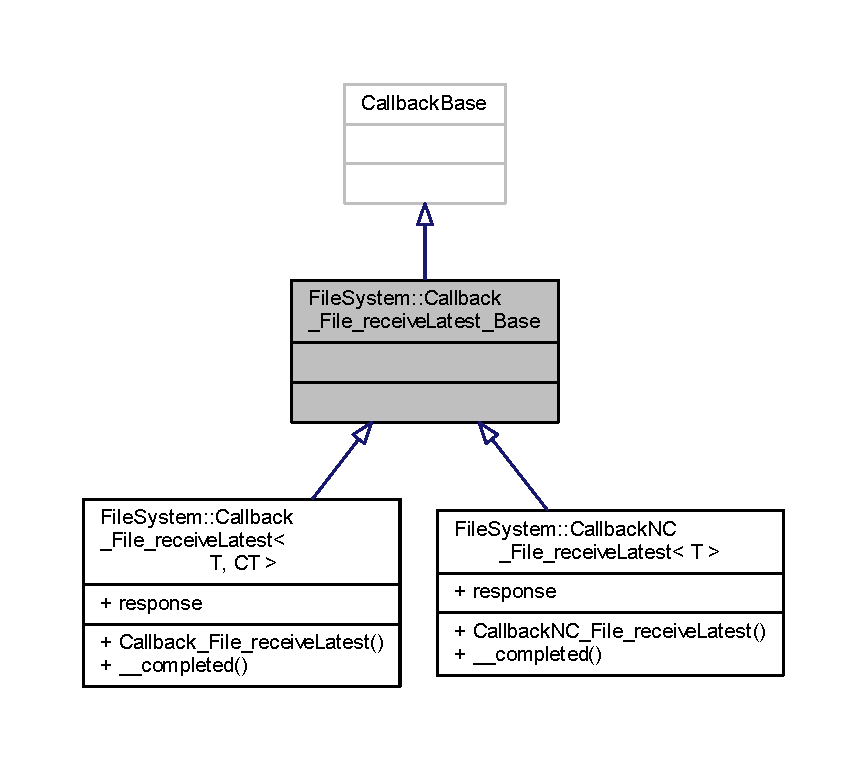
\includegraphics[width=350pt]{class_file_system_1_1_callback___file__receive_latest___base__inherit__graph}
\end{center}
\end{figure}


Collaboration diagram for File\+System\+:\+:Callback\+\_\+\+File\+\_\+receive\+Latest\+\_\+\+Base\+:
\nopagebreak
\begin{figure}[H]
\begin{center}
\leavevmode
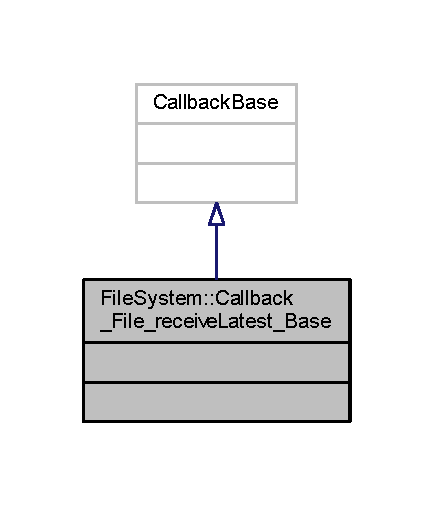
\includegraphics[width=208pt]{class_file_system_1_1_callback___file__receive_latest___base__coll__graph}
\end{center}
\end{figure}


The documentation for this class was generated from the following file\+:\begin{DoxyCompactItemize}
\item 
\hyperlink{_file_system_8h}{File\+System.\+h}\end{DoxyCompactItemize}

\hypertarget{class_file_system_1_1_callback___file__receive_version}{}\section{File\+System\+:\+:Callback\+\_\+\+File\+\_\+receive\+Version$<$ T, C\+T $>$ Class Template Reference}
\label{class_file_system_1_1_callback___file__receive_version}\index{File\+System\+::\+Callback\+\_\+\+File\+\_\+receive\+Version$<$ T, C\+T $>$@{File\+System\+::\+Callback\+\_\+\+File\+\_\+receive\+Version$<$ T, C\+T $>$}}


{\ttfamily \#include $<$File\+System.\+h$>$}



Inheritance diagram for File\+System\+:\+:Callback\+\_\+\+File\+\_\+receive\+Version$<$ T, C\+T $>$\+:
\nopagebreak
\begin{figure}[H]
\begin{center}
\leavevmode
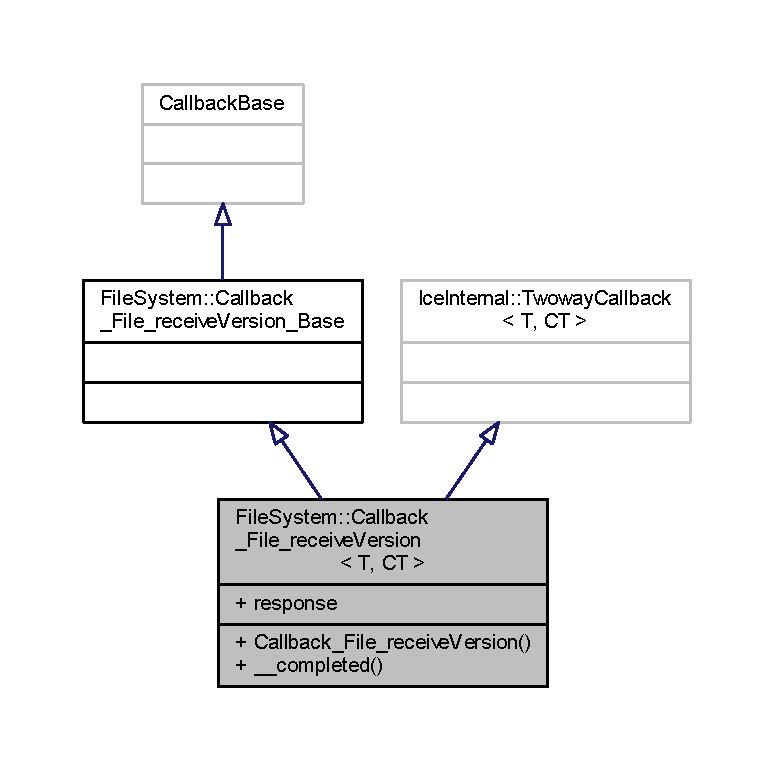
\includegraphics[width=350pt]{class_file_system_1_1_callback___file__receive_version__inherit__graph}
\end{center}
\end{figure}


Collaboration diagram for File\+System\+:\+:Callback\+\_\+\+File\+\_\+receive\+Version$<$ T, C\+T $>$\+:
\nopagebreak
\begin{figure}[H]
\begin{center}
\leavevmode
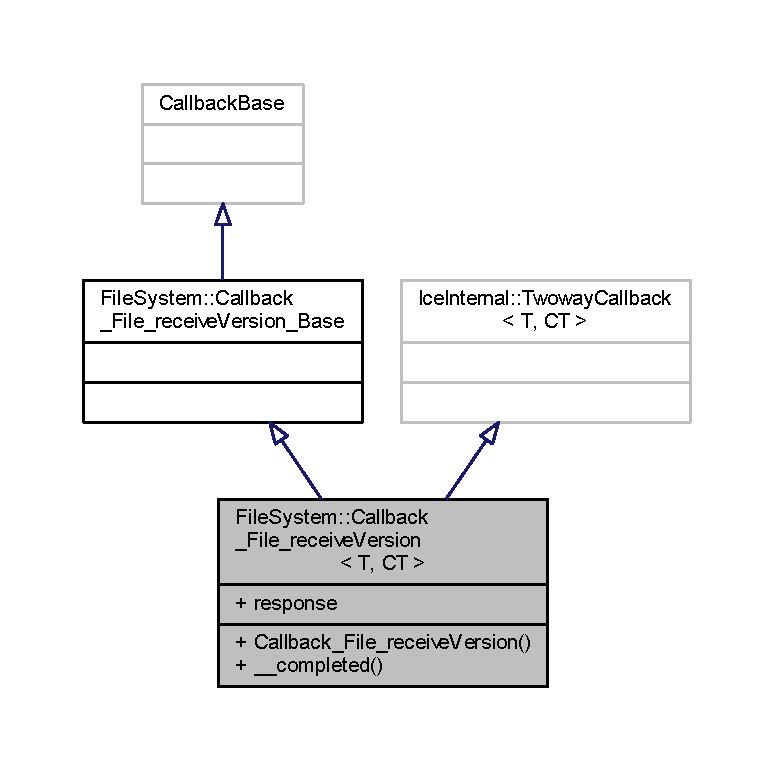
\includegraphics[width=350pt]{class_file_system_1_1_callback___file__receive_version__coll__graph}
\end{center}
\end{figure}
\subsection*{Public Types}
\begin{DoxyCompactItemize}
\item 
typedef Ice\+Util\+::\+Handle$<$ T $>$ \hyperlink{class_file_system_1_1_callback___file__receive_version_ad3c99b998d7a847dca7193dd3cad8cf1}{T\+Ptr}
\item 
typedef void(T\+::$\ast$ \hyperlink{class_file_system_1_1_callback___file__receive_version_a8ec034c43b3913243caf48c7de06f99d}{Exception}) (const \+::Ice\+::\+Exception \&, const C\+T \&)
\item 
typedef void(T\+::$\ast$ \hyperlink{class_file_system_1_1_callback___file__receive_version_a70f13401fd06a120da116b0b17ea67d0}{Sent}) (bool, const C\+T \&)
\item 
typedef void(T\+::$\ast$ \hyperlink{class_file_system_1_1_callback___file__receive_version_ab5743b6627d5fde356fc7381fcc4613a}{Response}) (const \+::\hyperlink{namespace_file_system_a5c85de065f9c451ae1d1dea2dacb68c5}{File\+System\+::\+Byte\+Seq} \&, const C\+T \&)
\end{DoxyCompactItemize}
\subsection*{Public Member Functions}
\begin{DoxyCompactItemize}
\item 
\hyperlink{class_file_system_1_1_callback___file__receive_version_a9502b37276feb5e696f8c52b718d2c15}{Callback\+\_\+\+File\+\_\+receive\+Version} (const \hyperlink{class_file_system_1_1_callback___file__receive_version_ad3c99b998d7a847dca7193dd3cad8cf1}{T\+Ptr} \&obj, \hyperlink{class_file_system_1_1_callback___file__receive_version_ab5743b6627d5fde356fc7381fcc4613a}{Response} cb, \hyperlink{class_file_system_1_1_callback___file__receive_version_a8ec034c43b3913243caf48c7de06f99d}{Exception} excb, \hyperlink{class_file_system_1_1_callback___file__receive_version_a70f13401fd06a120da116b0b17ea67d0}{Sent} sentcb)
\item 
virtual void \hyperlink{class_file_system_1_1_callback___file__receive_version_a76eea8d794fd8efa88cf529d77c04510}{\+\_\+\+\_\+completed} (const \+::Ice\+::\+Async\+Result\+Ptr \&\+\_\+\+\_\+result) const 
\end{DoxyCompactItemize}
\subsection*{Public Attributes}
\begin{DoxyCompactItemize}
\item 
\hyperlink{class_file_system_1_1_callback___file__receive_version_ab5743b6627d5fde356fc7381fcc4613a}{Response} \hyperlink{class_file_system_1_1_callback___file__receive_version_a8d059b5bb0d7ce620eb896bf2e3d32dc}{response}
\end{DoxyCompactItemize}


\subsection{Member Typedef Documentation}
\hypertarget{class_file_system_1_1_callback___file__receive_version_a8ec034c43b3913243caf48c7de06f99d}{}\index{File\+System\+::\+Callback\+\_\+\+File\+\_\+receive\+Version@{File\+System\+::\+Callback\+\_\+\+File\+\_\+receive\+Version}!Exception@{Exception}}
\index{Exception@{Exception}!File\+System\+::\+Callback\+\_\+\+File\+\_\+receive\+Version@{File\+System\+::\+Callback\+\_\+\+File\+\_\+receive\+Version}}
\subsubsection[{Exception}]{\setlength{\rightskip}{0pt plus 5cm}template$<$class T, typename C\+T$>$ typedef void(T\+::$\ast$ {\bf File\+System\+::\+Callback\+\_\+\+File\+\_\+receive\+Version}$<$ T, C\+T $>$\+::Exception) (const \+::Ice\+::\+Exception \&, const C\+T \&)}\label{class_file_system_1_1_callback___file__receive_version_a8ec034c43b3913243caf48c7de06f99d}
\hypertarget{class_file_system_1_1_callback___file__receive_version_ab5743b6627d5fde356fc7381fcc4613a}{}\index{File\+System\+::\+Callback\+\_\+\+File\+\_\+receive\+Version@{File\+System\+::\+Callback\+\_\+\+File\+\_\+receive\+Version}!Response@{Response}}
\index{Response@{Response}!File\+System\+::\+Callback\+\_\+\+File\+\_\+receive\+Version@{File\+System\+::\+Callback\+\_\+\+File\+\_\+receive\+Version}}
\subsubsection[{Response}]{\setlength{\rightskip}{0pt plus 5cm}template$<$class T, typename C\+T$>$ typedef void(T\+::$\ast$ {\bf File\+System\+::\+Callback\+\_\+\+File\+\_\+receive\+Version}$<$ T, C\+T $>$\+::Response) (const \+::{\bf File\+System\+::\+Byte\+Seq} \&, const C\+T \&)}\label{class_file_system_1_1_callback___file__receive_version_ab5743b6627d5fde356fc7381fcc4613a}
\hypertarget{class_file_system_1_1_callback___file__receive_version_a70f13401fd06a120da116b0b17ea67d0}{}\index{File\+System\+::\+Callback\+\_\+\+File\+\_\+receive\+Version@{File\+System\+::\+Callback\+\_\+\+File\+\_\+receive\+Version}!Sent@{Sent}}
\index{Sent@{Sent}!File\+System\+::\+Callback\+\_\+\+File\+\_\+receive\+Version@{File\+System\+::\+Callback\+\_\+\+File\+\_\+receive\+Version}}
\subsubsection[{Sent}]{\setlength{\rightskip}{0pt plus 5cm}template$<$class T, typename C\+T$>$ typedef void(T\+::$\ast$ {\bf File\+System\+::\+Callback\+\_\+\+File\+\_\+receive\+Version}$<$ T, C\+T $>$\+::Sent) (bool, const C\+T \&)}\label{class_file_system_1_1_callback___file__receive_version_a70f13401fd06a120da116b0b17ea67d0}
\hypertarget{class_file_system_1_1_callback___file__receive_version_ad3c99b998d7a847dca7193dd3cad8cf1}{}\index{File\+System\+::\+Callback\+\_\+\+File\+\_\+receive\+Version@{File\+System\+::\+Callback\+\_\+\+File\+\_\+receive\+Version}!T\+Ptr@{T\+Ptr}}
\index{T\+Ptr@{T\+Ptr}!File\+System\+::\+Callback\+\_\+\+File\+\_\+receive\+Version@{File\+System\+::\+Callback\+\_\+\+File\+\_\+receive\+Version}}
\subsubsection[{T\+Ptr}]{\setlength{\rightskip}{0pt plus 5cm}template$<$class T, typename C\+T$>$ typedef Ice\+Util\+::\+Handle$<$T$>$ {\bf File\+System\+::\+Callback\+\_\+\+File\+\_\+receive\+Version}$<$ T, C\+T $>$\+::{\bf T\+Ptr}}\label{class_file_system_1_1_callback___file__receive_version_ad3c99b998d7a847dca7193dd3cad8cf1}


\subsection{Constructor \& Destructor Documentation}
\hypertarget{class_file_system_1_1_callback___file__receive_version_a9502b37276feb5e696f8c52b718d2c15}{}\index{File\+System\+::\+Callback\+\_\+\+File\+\_\+receive\+Version@{File\+System\+::\+Callback\+\_\+\+File\+\_\+receive\+Version}!Callback\+\_\+\+File\+\_\+receive\+Version@{Callback\+\_\+\+File\+\_\+receive\+Version}}
\index{Callback\+\_\+\+File\+\_\+receive\+Version@{Callback\+\_\+\+File\+\_\+receive\+Version}!File\+System\+::\+Callback\+\_\+\+File\+\_\+receive\+Version@{File\+System\+::\+Callback\+\_\+\+File\+\_\+receive\+Version}}
\subsubsection[{Callback\+\_\+\+File\+\_\+receive\+Version}]{\setlength{\rightskip}{0pt plus 5cm}template$<$class T, typename C\+T$>$ {\bf File\+System\+::\+Callback\+\_\+\+File\+\_\+receive\+Version}$<$ T, C\+T $>$\+::{\bf Callback\+\_\+\+File\+\_\+receive\+Version} (
\begin{DoxyParamCaption}
\item[{const {\bf T\+Ptr} \&}]{obj, }
\item[{{\bf Response}}]{cb, }
\item[{{\bf Exception}}]{excb, }
\item[{{\bf Sent}}]{sentcb}
\end{DoxyParamCaption}
)\hspace{0.3cm}{\ttfamily [inline]}}\label{class_file_system_1_1_callback___file__receive_version_a9502b37276feb5e696f8c52b718d2c15}


\subsection{Member Function Documentation}
\hypertarget{class_file_system_1_1_callback___file__receive_version_a76eea8d794fd8efa88cf529d77c04510}{}\index{File\+System\+::\+Callback\+\_\+\+File\+\_\+receive\+Version@{File\+System\+::\+Callback\+\_\+\+File\+\_\+receive\+Version}!\+\_\+\+\_\+completed@{\+\_\+\+\_\+completed}}
\index{\+\_\+\+\_\+completed@{\+\_\+\+\_\+completed}!File\+System\+::\+Callback\+\_\+\+File\+\_\+receive\+Version@{File\+System\+::\+Callback\+\_\+\+File\+\_\+receive\+Version}}
\subsubsection[{\+\_\+\+\_\+completed}]{\setlength{\rightskip}{0pt plus 5cm}template$<$class T, typename C\+T$>$ virtual void {\bf File\+System\+::\+Callback\+\_\+\+File\+\_\+receive\+Version}$<$ T, C\+T $>$\+::\+\_\+\+\_\+completed (
\begin{DoxyParamCaption}
\item[{const \+::Ice\+::\+Async\+Result\+Ptr \&}]{\+\_\+\+\_\+result}
\end{DoxyParamCaption}
) const\hspace{0.3cm}{\ttfamily [inline]}, {\ttfamily [virtual]}}\label{class_file_system_1_1_callback___file__receive_version_a76eea8d794fd8efa88cf529d77c04510}


\subsection{Member Data Documentation}
\hypertarget{class_file_system_1_1_callback___file__receive_version_a8d059b5bb0d7ce620eb896bf2e3d32dc}{}\index{File\+System\+::\+Callback\+\_\+\+File\+\_\+receive\+Version@{File\+System\+::\+Callback\+\_\+\+File\+\_\+receive\+Version}!response@{response}}
\index{response@{response}!File\+System\+::\+Callback\+\_\+\+File\+\_\+receive\+Version@{File\+System\+::\+Callback\+\_\+\+File\+\_\+receive\+Version}}
\subsubsection[{response}]{\setlength{\rightskip}{0pt plus 5cm}template$<$class T, typename C\+T$>$ {\bf Response} {\bf File\+System\+::\+Callback\+\_\+\+File\+\_\+receive\+Version}$<$ T, C\+T $>$\+::response}\label{class_file_system_1_1_callback___file__receive_version_a8d059b5bb0d7ce620eb896bf2e3d32dc}


The documentation for this class was generated from the following file\+:\begin{DoxyCompactItemize}
\item 
\hyperlink{_file_system_8h}{File\+System.\+h}\end{DoxyCompactItemize}

\hypertarget{class_file_system_1_1_callback___file__receive_version___base}{}\section{File\+System\+:\+:Callback\+\_\+\+File\+\_\+receive\+Version\+\_\+\+Base Class Reference}
\label{class_file_system_1_1_callback___file__receive_version___base}\index{File\+System\+::\+Callback\+\_\+\+File\+\_\+receive\+Version\+\_\+\+Base@{File\+System\+::\+Callback\+\_\+\+File\+\_\+receive\+Version\+\_\+\+Base}}


{\ttfamily \#include $<$File\+System.\+h$>$}



Inheritance diagram for File\+System\+:\+:Callback\+\_\+\+File\+\_\+receive\+Version\+\_\+\+Base\+:
\nopagebreak
\begin{figure}[H]
\begin{center}
\leavevmode
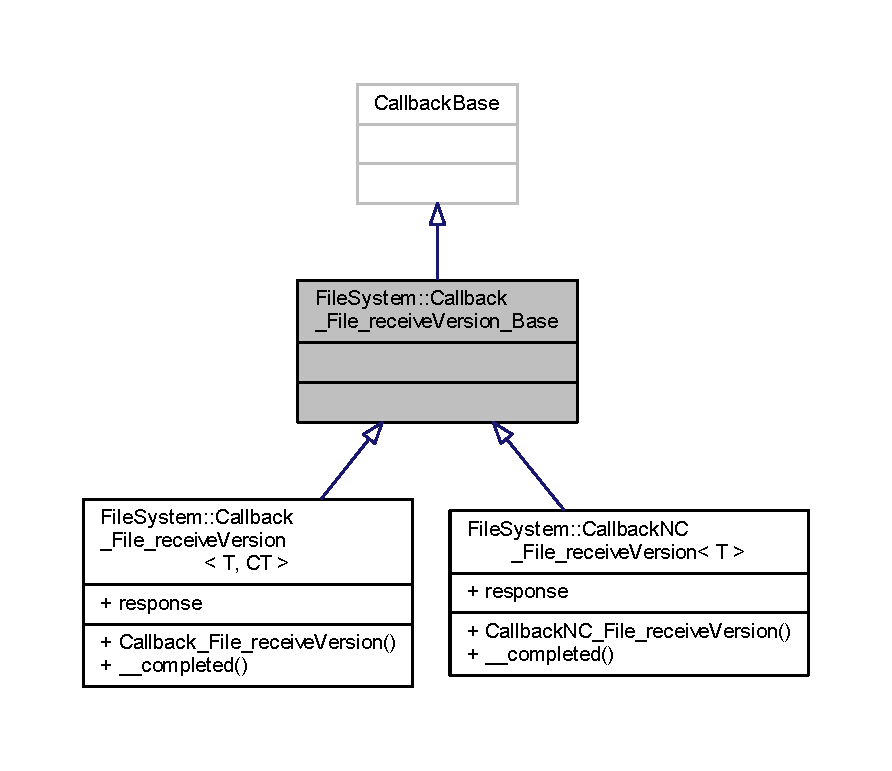
\includegraphics[width=350pt]{class_file_system_1_1_callback___file__receive_version___base__inherit__graph}
\end{center}
\end{figure}


Collaboration diagram for File\+System\+:\+:Callback\+\_\+\+File\+\_\+receive\+Version\+\_\+\+Base\+:
\nopagebreak
\begin{figure}[H]
\begin{center}
\leavevmode
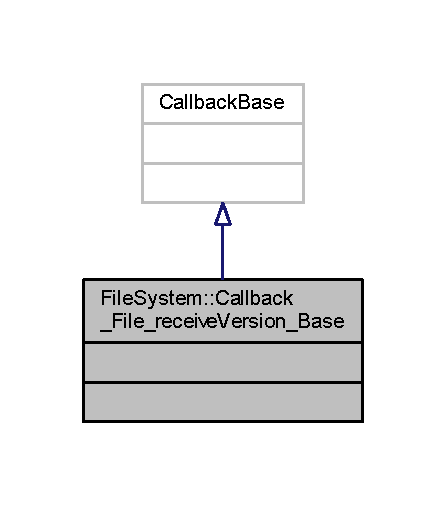
\includegraphics[width=214pt]{class_file_system_1_1_callback___file__receive_version___base__coll__graph}
\end{center}
\end{figure}


The documentation for this class was generated from the following file\+:\begin{DoxyCompactItemize}
\item 
\hyperlink{_file_system_8h}{File\+System.\+h}\end{DoxyCompactItemize}

\hypertarget{class_file_system_1_1_callback___file__send_file}{}\section{File\+System\+:\+:Callback\+\_\+\+File\+\_\+send\+File$<$ T, C\+T $>$ Class Template Reference}
\label{class_file_system_1_1_callback___file__send_file}\index{File\+System\+::\+Callback\+\_\+\+File\+\_\+send\+File$<$ T, C\+T $>$@{File\+System\+::\+Callback\+\_\+\+File\+\_\+send\+File$<$ T, C\+T $>$}}


{\ttfamily \#include $<$File\+System.\+h$>$}



Inheritance diagram for File\+System\+:\+:Callback\+\_\+\+File\+\_\+send\+File$<$ T, C\+T $>$\+:
\nopagebreak
\begin{figure}[H]
\begin{center}
\leavevmode
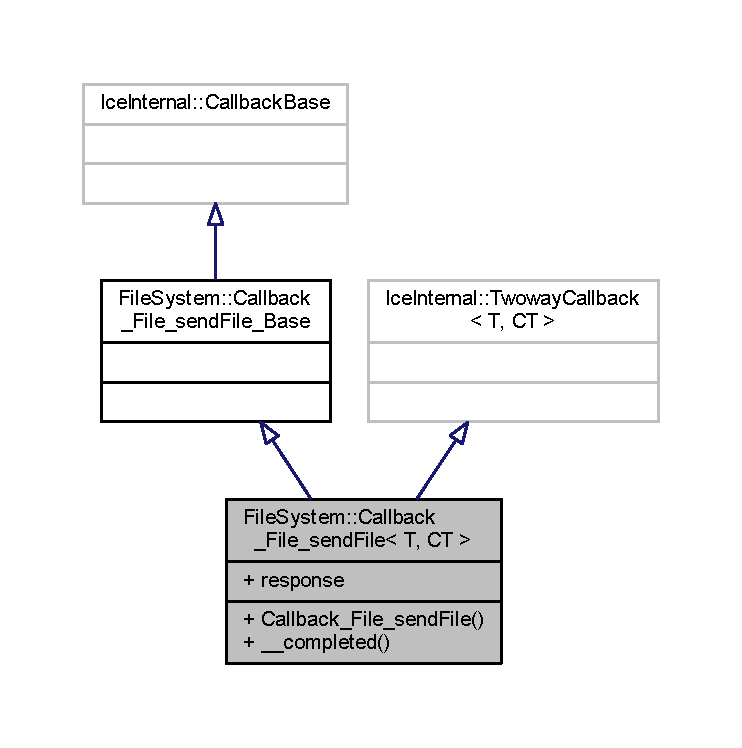
\includegraphics[width=350pt]{class_file_system_1_1_callback___file__send_file__inherit__graph}
\end{center}
\end{figure}


Collaboration diagram for File\+System\+:\+:Callback\+\_\+\+File\+\_\+send\+File$<$ T, C\+T $>$\+:
\nopagebreak
\begin{figure}[H]
\begin{center}
\leavevmode
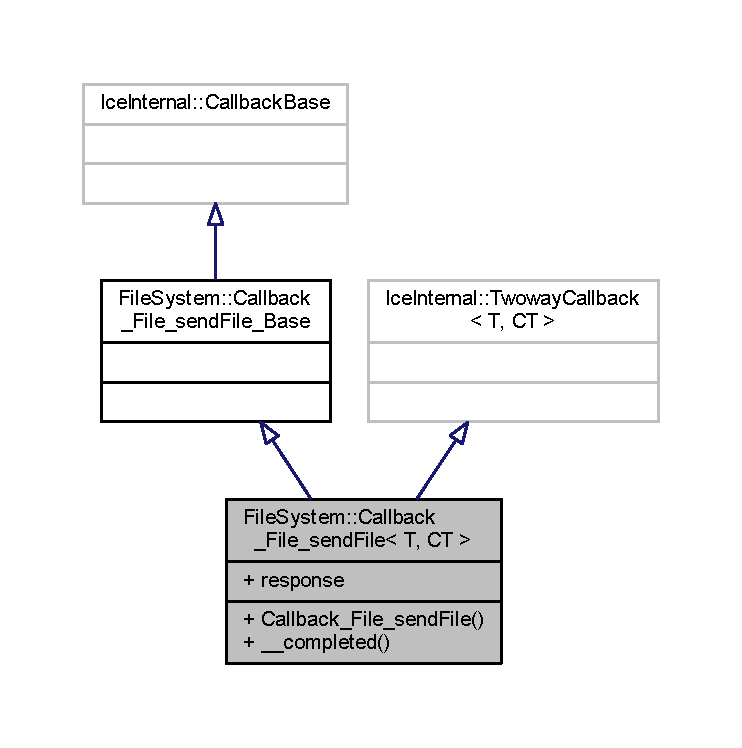
\includegraphics[width=350pt]{class_file_system_1_1_callback___file__send_file__coll__graph}
\end{center}
\end{figure}
\subsection*{Public Types}
\begin{DoxyCompactItemize}
\item 
typedef Ice\+Util\+::\+Handle$<$ T $>$ \hyperlink{class_file_system_1_1_callback___file__send_file_a666a8ba5af39dac36fdcb52b0916e2b9}{T\+Ptr}
\item 
typedef void(T\+::$\ast$ \hyperlink{class_file_system_1_1_callback___file__send_file_a625b27b53ceb949eaa41ae4908958999}{Exception}) (const \+::Ice\+::\+Exception \&, const C\+T \&)
\item 
typedef void(T\+::$\ast$ \hyperlink{class_file_system_1_1_callback___file__send_file_ac3926735f3de742485a01c7e0e08dd2d}{Sent}) (bool, const C\+T \&)
\item 
typedef void(T\+::$\ast$ \hyperlink{class_file_system_1_1_callback___file__send_file_a3d604d3396d90e28e0f498d66e31e906}{Response}) (bool, const C\+T \&)
\end{DoxyCompactItemize}
\subsection*{Public Member Functions}
\begin{DoxyCompactItemize}
\item 
\hyperlink{class_file_system_1_1_callback___file__send_file_a5dfd7d4e2727b7b8be3f1aab6b57124a}{Callback\+\_\+\+File\+\_\+send\+File} (const \hyperlink{class_file_system_1_1_callback___file__send_file_a666a8ba5af39dac36fdcb52b0916e2b9}{T\+Ptr} \&obj, \hyperlink{class_file_system_1_1_callback___file__send_file_a3d604d3396d90e28e0f498d66e31e906}{Response} cb, \hyperlink{class_file_system_1_1_callback___file__send_file_a625b27b53ceb949eaa41ae4908958999}{Exception} excb, \hyperlink{class_file_system_1_1_callback___file__send_file_ac3926735f3de742485a01c7e0e08dd2d}{Sent} sentcb)
\item 
virtual void \hyperlink{class_file_system_1_1_callback___file__send_file_a8272471d8bad3733858c33daf74bf1a7}{\+\_\+\+\_\+completed} (const \+::Ice\+::\+Async\+Result\+Ptr \&\+\_\+\+\_\+result) const 
\end{DoxyCompactItemize}
\subsection*{Public Attributes}
\begin{DoxyCompactItemize}
\item 
\hyperlink{class_file_system_1_1_callback___file__send_file_a3d604d3396d90e28e0f498d66e31e906}{Response} \hyperlink{class_file_system_1_1_callback___file__send_file_a5a393b1e37b7cd16f4154ca5c91af37e}{response}
\end{DoxyCompactItemize}


\subsection{Member Typedef Documentation}
\hypertarget{class_file_system_1_1_callback___file__send_file_a625b27b53ceb949eaa41ae4908958999}{}\index{File\+System\+::\+Callback\+\_\+\+File\+\_\+send\+File@{File\+System\+::\+Callback\+\_\+\+File\+\_\+send\+File}!Exception@{Exception}}
\index{Exception@{Exception}!File\+System\+::\+Callback\+\_\+\+File\+\_\+send\+File@{File\+System\+::\+Callback\+\_\+\+File\+\_\+send\+File}}
\subsubsection[{Exception}]{\setlength{\rightskip}{0pt plus 5cm}template$<$class T, typename C\+T$>$ typedef void(T\+::$\ast$ {\bf File\+System\+::\+Callback\+\_\+\+File\+\_\+send\+File}$<$ T, C\+T $>$\+::Exception) (const \+::Ice\+::\+Exception \&, const C\+T \&)}\label{class_file_system_1_1_callback___file__send_file_a625b27b53ceb949eaa41ae4908958999}
\hypertarget{class_file_system_1_1_callback___file__send_file_a3d604d3396d90e28e0f498d66e31e906}{}\index{File\+System\+::\+Callback\+\_\+\+File\+\_\+send\+File@{File\+System\+::\+Callback\+\_\+\+File\+\_\+send\+File}!Response@{Response}}
\index{Response@{Response}!File\+System\+::\+Callback\+\_\+\+File\+\_\+send\+File@{File\+System\+::\+Callback\+\_\+\+File\+\_\+send\+File}}
\subsubsection[{Response}]{\setlength{\rightskip}{0pt plus 5cm}template$<$class T, typename C\+T$>$ typedef void(T\+::$\ast$ {\bf File\+System\+::\+Callback\+\_\+\+File\+\_\+send\+File}$<$ T, C\+T $>$\+::Response) (bool, const C\+T \&)}\label{class_file_system_1_1_callback___file__send_file_a3d604d3396d90e28e0f498d66e31e906}
\hypertarget{class_file_system_1_1_callback___file__send_file_ac3926735f3de742485a01c7e0e08dd2d}{}\index{File\+System\+::\+Callback\+\_\+\+File\+\_\+send\+File@{File\+System\+::\+Callback\+\_\+\+File\+\_\+send\+File}!Sent@{Sent}}
\index{Sent@{Sent}!File\+System\+::\+Callback\+\_\+\+File\+\_\+send\+File@{File\+System\+::\+Callback\+\_\+\+File\+\_\+send\+File}}
\subsubsection[{Sent}]{\setlength{\rightskip}{0pt plus 5cm}template$<$class T, typename C\+T$>$ typedef void(T\+::$\ast$ {\bf File\+System\+::\+Callback\+\_\+\+File\+\_\+send\+File}$<$ T, C\+T $>$\+::Sent) (bool, const C\+T \&)}\label{class_file_system_1_1_callback___file__send_file_ac3926735f3de742485a01c7e0e08dd2d}
\hypertarget{class_file_system_1_1_callback___file__send_file_a666a8ba5af39dac36fdcb52b0916e2b9}{}\index{File\+System\+::\+Callback\+\_\+\+File\+\_\+send\+File@{File\+System\+::\+Callback\+\_\+\+File\+\_\+send\+File}!T\+Ptr@{T\+Ptr}}
\index{T\+Ptr@{T\+Ptr}!File\+System\+::\+Callback\+\_\+\+File\+\_\+send\+File@{File\+System\+::\+Callback\+\_\+\+File\+\_\+send\+File}}
\subsubsection[{T\+Ptr}]{\setlength{\rightskip}{0pt plus 5cm}template$<$class T, typename C\+T$>$ typedef Ice\+Util\+::\+Handle$<$T$>$ {\bf File\+System\+::\+Callback\+\_\+\+File\+\_\+send\+File}$<$ T, C\+T $>$\+::{\bf T\+Ptr}}\label{class_file_system_1_1_callback___file__send_file_a666a8ba5af39dac36fdcb52b0916e2b9}


\subsection{Constructor \& Destructor Documentation}
\hypertarget{class_file_system_1_1_callback___file__send_file_a5dfd7d4e2727b7b8be3f1aab6b57124a}{}\index{File\+System\+::\+Callback\+\_\+\+File\+\_\+send\+File@{File\+System\+::\+Callback\+\_\+\+File\+\_\+send\+File}!Callback\+\_\+\+File\+\_\+send\+File@{Callback\+\_\+\+File\+\_\+send\+File}}
\index{Callback\+\_\+\+File\+\_\+send\+File@{Callback\+\_\+\+File\+\_\+send\+File}!File\+System\+::\+Callback\+\_\+\+File\+\_\+send\+File@{File\+System\+::\+Callback\+\_\+\+File\+\_\+send\+File}}
\subsubsection[{Callback\+\_\+\+File\+\_\+send\+File}]{\setlength{\rightskip}{0pt plus 5cm}template$<$class T, typename C\+T$>$ {\bf File\+System\+::\+Callback\+\_\+\+File\+\_\+send\+File}$<$ T, C\+T $>$\+::{\bf Callback\+\_\+\+File\+\_\+send\+File} (
\begin{DoxyParamCaption}
\item[{const {\bf T\+Ptr} \&}]{obj, }
\item[{{\bf Response}}]{cb, }
\item[{{\bf Exception}}]{excb, }
\item[{{\bf Sent}}]{sentcb}
\end{DoxyParamCaption}
)\hspace{0.3cm}{\ttfamily [inline]}}\label{class_file_system_1_1_callback___file__send_file_a5dfd7d4e2727b7b8be3f1aab6b57124a}


\subsection{Member Function Documentation}
\hypertarget{class_file_system_1_1_callback___file__send_file_a8272471d8bad3733858c33daf74bf1a7}{}\index{File\+System\+::\+Callback\+\_\+\+File\+\_\+send\+File@{File\+System\+::\+Callback\+\_\+\+File\+\_\+send\+File}!\+\_\+\+\_\+completed@{\+\_\+\+\_\+completed}}
\index{\+\_\+\+\_\+completed@{\+\_\+\+\_\+completed}!File\+System\+::\+Callback\+\_\+\+File\+\_\+send\+File@{File\+System\+::\+Callback\+\_\+\+File\+\_\+send\+File}}
\subsubsection[{\+\_\+\+\_\+completed}]{\setlength{\rightskip}{0pt plus 5cm}template$<$class T, typename C\+T$>$ virtual void {\bf File\+System\+::\+Callback\+\_\+\+File\+\_\+send\+File}$<$ T, C\+T $>$\+::\+\_\+\+\_\+completed (
\begin{DoxyParamCaption}
\item[{const \+::Ice\+::\+Async\+Result\+Ptr \&}]{\+\_\+\+\_\+result}
\end{DoxyParamCaption}
) const\hspace{0.3cm}{\ttfamily [inline]}, {\ttfamily [virtual]}}\label{class_file_system_1_1_callback___file__send_file_a8272471d8bad3733858c33daf74bf1a7}


\subsection{Member Data Documentation}
\hypertarget{class_file_system_1_1_callback___file__send_file_a5a393b1e37b7cd16f4154ca5c91af37e}{}\index{File\+System\+::\+Callback\+\_\+\+File\+\_\+send\+File@{File\+System\+::\+Callback\+\_\+\+File\+\_\+send\+File}!response@{response}}
\index{response@{response}!File\+System\+::\+Callback\+\_\+\+File\+\_\+send\+File@{File\+System\+::\+Callback\+\_\+\+File\+\_\+send\+File}}
\subsubsection[{response}]{\setlength{\rightskip}{0pt plus 5cm}template$<$class T, typename C\+T$>$ {\bf Response} {\bf File\+System\+::\+Callback\+\_\+\+File\+\_\+send\+File}$<$ T, C\+T $>$\+::response}\label{class_file_system_1_1_callback___file__send_file_a5a393b1e37b7cd16f4154ca5c91af37e}


The documentation for this class was generated from the following file\+:\begin{DoxyCompactItemize}
\item 
\hyperlink{_file_system_8h}{File\+System.\+h}\end{DoxyCompactItemize}

\hypertarget{class_file_system_1_1_callback___file__send_file___base}{}\section{File\+System\+:\+:Callback\+\_\+\+File\+\_\+send\+File\+\_\+\+Base Class Reference}
\label{class_file_system_1_1_callback___file__send_file___base}\index{File\+System\+::\+Callback\+\_\+\+File\+\_\+send\+File\+\_\+\+Base@{File\+System\+::\+Callback\+\_\+\+File\+\_\+send\+File\+\_\+\+Base}}


{\ttfamily \#include $<$File\+System.\+h$>$}



Inheritance diagram for File\+System\+:\+:Callback\+\_\+\+File\+\_\+send\+File\+\_\+\+Base\+:
\nopagebreak
\begin{figure}[H]
\begin{center}
\leavevmode
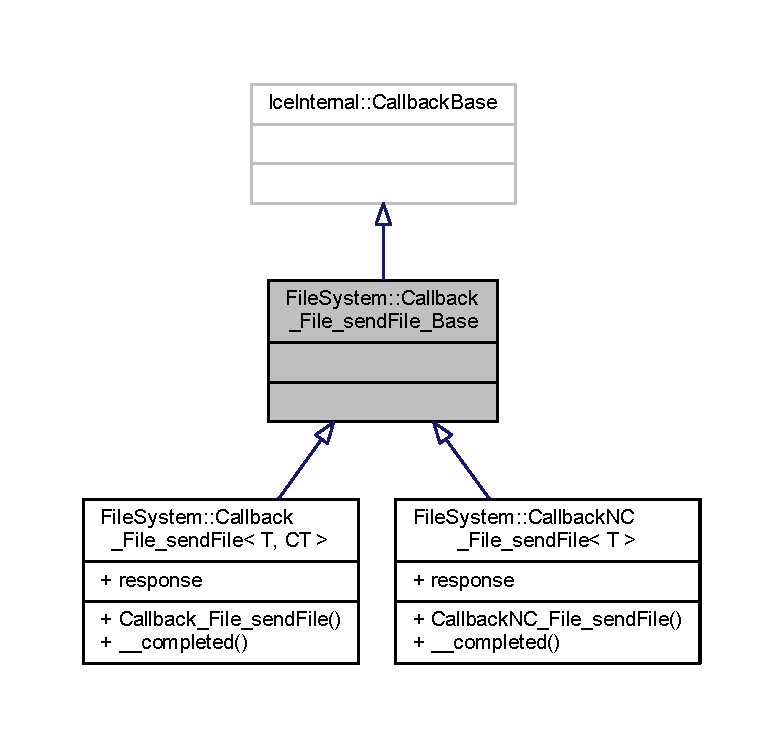
\includegraphics[width=350pt]{class_file_system_1_1_callback___file__send_file___base__inherit__graph}
\end{center}
\end{figure}


Collaboration diagram for File\+System\+:\+:Callback\+\_\+\+File\+\_\+send\+File\+\_\+\+Base\+:
\nopagebreak
\begin{figure}[H]
\begin{center}
\leavevmode
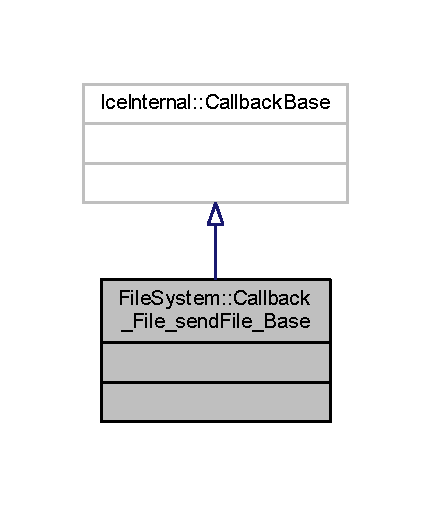
\includegraphics[width=207pt]{class_file_system_1_1_callback___file__send_file___base__coll__graph}
\end{center}
\end{figure}


The documentation for this class was generated from the following file\+:\begin{DoxyCompactItemize}
\item 
\hyperlink{_file_system_8h}{File\+System.\+h}\end{DoxyCompactItemize}

\hypertarget{class_file_system_1_1_callback_n_c___file__get_history}{}\section{File\+System\+:\+:Callback\+N\+C\+\_\+\+File\+\_\+get\+History$<$ T $>$ Class Template Reference}
\label{class_file_system_1_1_callback_n_c___file__get_history}\index{File\+System\+::\+Callback\+N\+C\+\_\+\+File\+\_\+get\+History$<$ T $>$@{File\+System\+::\+Callback\+N\+C\+\_\+\+File\+\_\+get\+History$<$ T $>$}}


{\ttfamily \#include $<$File\+System.\+h$>$}



Inheritance diagram for File\+System\+:\+:Callback\+N\+C\+\_\+\+File\+\_\+get\+History$<$ T $>$\+:
\nopagebreak
\begin{figure}[H]
\begin{center}
\leavevmode
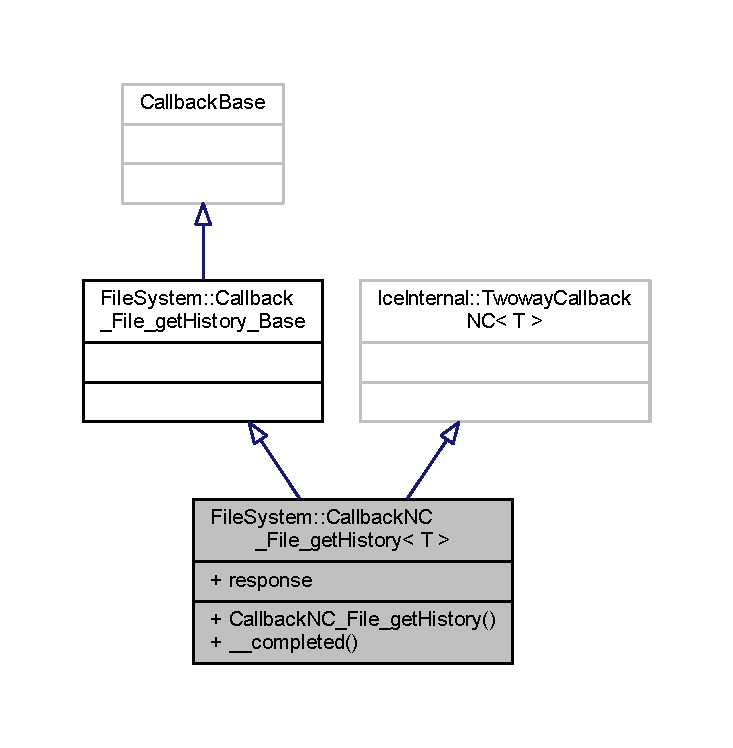
\includegraphics[width=350pt]{class_file_system_1_1_callback_n_c___file__get_history__inherit__graph}
\end{center}
\end{figure}


Collaboration diagram for File\+System\+:\+:Callback\+N\+C\+\_\+\+File\+\_\+get\+History$<$ T $>$\+:
\nopagebreak
\begin{figure}[H]
\begin{center}
\leavevmode
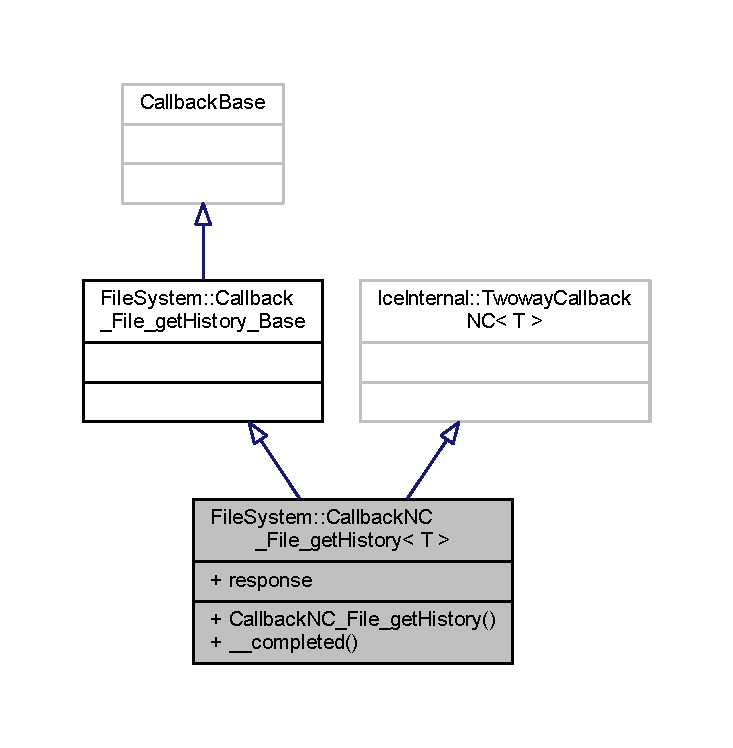
\includegraphics[width=350pt]{class_file_system_1_1_callback_n_c___file__get_history__coll__graph}
\end{center}
\end{figure}
\subsection*{Public Types}
\begin{DoxyCompactItemize}
\item 
typedef Ice\+Util\+::\+Handle$<$ T $>$ \hyperlink{class_file_system_1_1_callback_n_c___file__get_history_ae005e81d63a5bdcf9b9aafc40a28ff6b}{T\+Ptr}
\item 
typedef void(T\+::$\ast$ \hyperlink{class_file_system_1_1_callback_n_c___file__get_history_a828dbde2a7dd89e32a5e98ea6a92c9a7}{Exception}) (const \+::Ice\+::\+Exception \&)
\item 
typedef void(T\+::$\ast$ \hyperlink{class_file_system_1_1_callback_n_c___file__get_history_a9e909ff9b45d83e890c037566c529f6e}{Sent}) (bool)
\item 
typedef void(T\+::$\ast$ \hyperlink{class_file_system_1_1_callback_n_c___file__get_history_a7fef6c01133235ae7b604366d356eae4}{Response}) (const \+::\hyperlink{namespace_file_system_ac32dc1eb34c060160b52edc7c4e37d6e}{File\+System\+::\+Ver\+Seq} \&)
\end{DoxyCompactItemize}
\subsection*{Public Member Functions}
\begin{DoxyCompactItemize}
\item 
\hyperlink{class_file_system_1_1_callback_n_c___file__get_history_ae52fe43d18b6869f34b2c64d10f6b91e}{Callback\+N\+C\+\_\+\+File\+\_\+get\+History} (const \hyperlink{class_file_system_1_1_callback_n_c___file__get_history_ae005e81d63a5bdcf9b9aafc40a28ff6b}{T\+Ptr} \&obj, \hyperlink{class_file_system_1_1_callback_n_c___file__get_history_a7fef6c01133235ae7b604366d356eae4}{Response} cb, \hyperlink{class_file_system_1_1_callback_n_c___file__get_history_a828dbde2a7dd89e32a5e98ea6a92c9a7}{Exception} excb, \hyperlink{class_file_system_1_1_callback_n_c___file__get_history_a9e909ff9b45d83e890c037566c529f6e}{Sent} sentcb)
\item 
virtual void \hyperlink{class_file_system_1_1_callback_n_c___file__get_history_a50cc232102d6f3cbc98da14381058b98}{\+\_\+\+\_\+completed} (const \+::Ice\+::\+Async\+Result\+Ptr \&\+\_\+\+\_\+result) const 
\end{DoxyCompactItemize}
\subsection*{Public Attributes}
\begin{DoxyCompactItemize}
\item 
\hyperlink{class_file_system_1_1_callback_n_c___file__get_history_a7fef6c01133235ae7b604366d356eae4}{Response} \hyperlink{class_file_system_1_1_callback_n_c___file__get_history_a81615ddfea371f53f4227fba28da454f}{response}
\end{DoxyCompactItemize}


\subsection{Member Typedef Documentation}
\hypertarget{class_file_system_1_1_callback_n_c___file__get_history_a828dbde2a7dd89e32a5e98ea6a92c9a7}{}\index{File\+System\+::\+Callback\+N\+C\+\_\+\+File\+\_\+get\+History@{File\+System\+::\+Callback\+N\+C\+\_\+\+File\+\_\+get\+History}!Exception@{Exception}}
\index{Exception@{Exception}!File\+System\+::\+Callback\+N\+C\+\_\+\+File\+\_\+get\+History@{File\+System\+::\+Callback\+N\+C\+\_\+\+File\+\_\+get\+History}}
\subsubsection[{Exception}]{\setlength{\rightskip}{0pt plus 5cm}template$<$class T$>$ typedef void(T\+::$\ast$ {\bf File\+System\+::\+Callback\+N\+C\+\_\+\+File\+\_\+get\+History}$<$ T $>$\+::Exception) (const \+::Ice\+::\+Exception \&)}\label{class_file_system_1_1_callback_n_c___file__get_history_a828dbde2a7dd89e32a5e98ea6a92c9a7}
\hypertarget{class_file_system_1_1_callback_n_c___file__get_history_a7fef6c01133235ae7b604366d356eae4}{}\index{File\+System\+::\+Callback\+N\+C\+\_\+\+File\+\_\+get\+History@{File\+System\+::\+Callback\+N\+C\+\_\+\+File\+\_\+get\+History}!Response@{Response}}
\index{Response@{Response}!File\+System\+::\+Callback\+N\+C\+\_\+\+File\+\_\+get\+History@{File\+System\+::\+Callback\+N\+C\+\_\+\+File\+\_\+get\+History}}
\subsubsection[{Response}]{\setlength{\rightskip}{0pt plus 5cm}template$<$class T$>$ typedef void(T\+::$\ast$ {\bf File\+System\+::\+Callback\+N\+C\+\_\+\+File\+\_\+get\+History}$<$ T $>$\+::Response) (const \+::{\bf File\+System\+::\+Ver\+Seq} \&)}\label{class_file_system_1_1_callback_n_c___file__get_history_a7fef6c01133235ae7b604366d356eae4}
\hypertarget{class_file_system_1_1_callback_n_c___file__get_history_a9e909ff9b45d83e890c037566c529f6e}{}\index{File\+System\+::\+Callback\+N\+C\+\_\+\+File\+\_\+get\+History@{File\+System\+::\+Callback\+N\+C\+\_\+\+File\+\_\+get\+History}!Sent@{Sent}}
\index{Sent@{Sent}!File\+System\+::\+Callback\+N\+C\+\_\+\+File\+\_\+get\+History@{File\+System\+::\+Callback\+N\+C\+\_\+\+File\+\_\+get\+History}}
\subsubsection[{Sent}]{\setlength{\rightskip}{0pt plus 5cm}template$<$class T$>$ typedef void(T\+::$\ast$ {\bf File\+System\+::\+Callback\+N\+C\+\_\+\+File\+\_\+get\+History}$<$ T $>$\+::Sent) (bool)}\label{class_file_system_1_1_callback_n_c___file__get_history_a9e909ff9b45d83e890c037566c529f6e}
\hypertarget{class_file_system_1_1_callback_n_c___file__get_history_ae005e81d63a5bdcf9b9aafc40a28ff6b}{}\index{File\+System\+::\+Callback\+N\+C\+\_\+\+File\+\_\+get\+History@{File\+System\+::\+Callback\+N\+C\+\_\+\+File\+\_\+get\+History}!T\+Ptr@{T\+Ptr}}
\index{T\+Ptr@{T\+Ptr}!File\+System\+::\+Callback\+N\+C\+\_\+\+File\+\_\+get\+History@{File\+System\+::\+Callback\+N\+C\+\_\+\+File\+\_\+get\+History}}
\subsubsection[{T\+Ptr}]{\setlength{\rightskip}{0pt plus 5cm}template$<$class T$>$ typedef Ice\+Util\+::\+Handle$<$T$>$ {\bf File\+System\+::\+Callback\+N\+C\+\_\+\+File\+\_\+get\+History}$<$ T $>$\+::{\bf T\+Ptr}}\label{class_file_system_1_1_callback_n_c___file__get_history_ae005e81d63a5bdcf9b9aafc40a28ff6b}


\subsection{Constructor \& Destructor Documentation}
\hypertarget{class_file_system_1_1_callback_n_c___file__get_history_ae52fe43d18b6869f34b2c64d10f6b91e}{}\index{File\+System\+::\+Callback\+N\+C\+\_\+\+File\+\_\+get\+History@{File\+System\+::\+Callback\+N\+C\+\_\+\+File\+\_\+get\+History}!Callback\+N\+C\+\_\+\+File\+\_\+get\+History@{Callback\+N\+C\+\_\+\+File\+\_\+get\+History}}
\index{Callback\+N\+C\+\_\+\+File\+\_\+get\+History@{Callback\+N\+C\+\_\+\+File\+\_\+get\+History}!File\+System\+::\+Callback\+N\+C\+\_\+\+File\+\_\+get\+History@{File\+System\+::\+Callback\+N\+C\+\_\+\+File\+\_\+get\+History}}
\subsubsection[{Callback\+N\+C\+\_\+\+File\+\_\+get\+History}]{\setlength{\rightskip}{0pt plus 5cm}template$<$class T$>$ {\bf File\+System\+::\+Callback\+N\+C\+\_\+\+File\+\_\+get\+History}$<$ T $>$\+::{\bf Callback\+N\+C\+\_\+\+File\+\_\+get\+History} (
\begin{DoxyParamCaption}
\item[{const {\bf T\+Ptr} \&}]{obj, }
\item[{{\bf Response}}]{cb, }
\item[{{\bf Exception}}]{excb, }
\item[{{\bf Sent}}]{sentcb}
\end{DoxyParamCaption}
)\hspace{0.3cm}{\ttfamily [inline]}}\label{class_file_system_1_1_callback_n_c___file__get_history_ae52fe43d18b6869f34b2c64d10f6b91e}


\subsection{Member Function Documentation}
\hypertarget{class_file_system_1_1_callback_n_c___file__get_history_a50cc232102d6f3cbc98da14381058b98}{}\index{File\+System\+::\+Callback\+N\+C\+\_\+\+File\+\_\+get\+History@{File\+System\+::\+Callback\+N\+C\+\_\+\+File\+\_\+get\+History}!\+\_\+\+\_\+completed@{\+\_\+\+\_\+completed}}
\index{\+\_\+\+\_\+completed@{\+\_\+\+\_\+completed}!File\+System\+::\+Callback\+N\+C\+\_\+\+File\+\_\+get\+History@{File\+System\+::\+Callback\+N\+C\+\_\+\+File\+\_\+get\+History}}
\subsubsection[{\+\_\+\+\_\+completed}]{\setlength{\rightskip}{0pt plus 5cm}template$<$class T$>$ virtual void {\bf File\+System\+::\+Callback\+N\+C\+\_\+\+File\+\_\+get\+History}$<$ T $>$\+::\+\_\+\+\_\+completed (
\begin{DoxyParamCaption}
\item[{const \+::Ice\+::\+Async\+Result\+Ptr \&}]{\+\_\+\+\_\+result}
\end{DoxyParamCaption}
) const\hspace{0.3cm}{\ttfamily [inline]}, {\ttfamily [virtual]}}\label{class_file_system_1_1_callback_n_c___file__get_history_a50cc232102d6f3cbc98da14381058b98}


\subsection{Member Data Documentation}
\hypertarget{class_file_system_1_1_callback_n_c___file__get_history_a81615ddfea371f53f4227fba28da454f}{}\index{File\+System\+::\+Callback\+N\+C\+\_\+\+File\+\_\+get\+History@{File\+System\+::\+Callback\+N\+C\+\_\+\+File\+\_\+get\+History}!response@{response}}
\index{response@{response}!File\+System\+::\+Callback\+N\+C\+\_\+\+File\+\_\+get\+History@{File\+System\+::\+Callback\+N\+C\+\_\+\+File\+\_\+get\+History}}
\subsubsection[{response}]{\setlength{\rightskip}{0pt plus 5cm}template$<$class T$>$ {\bf Response} {\bf File\+System\+::\+Callback\+N\+C\+\_\+\+File\+\_\+get\+History}$<$ T $>$\+::response}\label{class_file_system_1_1_callback_n_c___file__get_history_a81615ddfea371f53f4227fba28da454f}


The documentation for this class was generated from the following file\+:\begin{DoxyCompactItemize}
\item 
\hyperlink{_file_system_8h}{File\+System.\+h}\end{DoxyCompactItemize}

\hypertarget{class_file_system_1_1_callback_n_c___file__receive_latest}{}\section{File\+System\+:\+:Callback\+N\+C\+\_\+\+File\+\_\+receive\+Latest$<$ T $>$ Class Template Reference}
\label{class_file_system_1_1_callback_n_c___file__receive_latest}\index{File\+System\+::\+Callback\+N\+C\+\_\+\+File\+\_\+receive\+Latest$<$ T $>$@{File\+System\+::\+Callback\+N\+C\+\_\+\+File\+\_\+receive\+Latest$<$ T $>$}}


{\ttfamily \#include $<$File\+System.\+h$>$}



Inheritance diagram for File\+System\+:\+:Callback\+N\+C\+\_\+\+File\+\_\+receive\+Latest$<$ T $>$\+:
\nopagebreak
\begin{figure}[H]
\begin{center}
\leavevmode
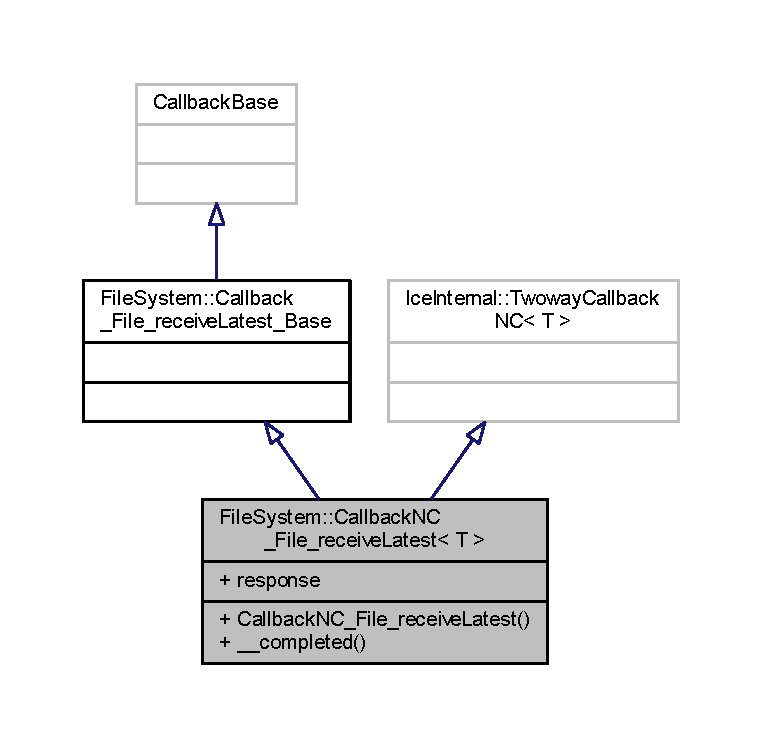
\includegraphics[width=350pt]{class_file_system_1_1_callback_n_c___file__receive_latest__inherit__graph}
\end{center}
\end{figure}


Collaboration diagram for File\+System\+:\+:Callback\+N\+C\+\_\+\+File\+\_\+receive\+Latest$<$ T $>$\+:
\nopagebreak
\begin{figure}[H]
\begin{center}
\leavevmode
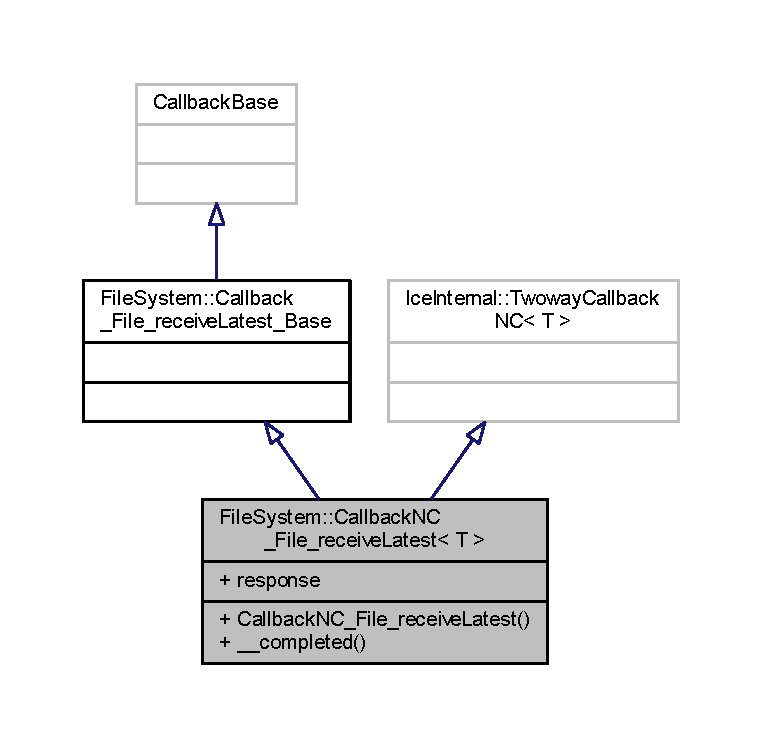
\includegraphics[width=350pt]{class_file_system_1_1_callback_n_c___file__receive_latest__coll__graph}
\end{center}
\end{figure}
\subsection*{Public Types}
\begin{DoxyCompactItemize}
\item 
typedef Ice\+Util\+::\+Handle$<$ T $>$ \hyperlink{class_file_system_1_1_callback_n_c___file__receive_latest_afbae5443c9515ea0676fd1201dd9eb20}{T\+Ptr}
\item 
typedef void(T\+::$\ast$ \hyperlink{class_file_system_1_1_callback_n_c___file__receive_latest_ab30d613e7021d1b46736b1249e24dd79}{Exception}) (const \+::Ice\+::\+Exception \&)
\item 
typedef void(T\+::$\ast$ \hyperlink{class_file_system_1_1_callback_n_c___file__receive_latest_a5eb8166c1545749bdf317b280f2aff67}{Sent}) (bool)
\item 
typedef void(T\+::$\ast$ \hyperlink{class_file_system_1_1_callback_n_c___file__receive_latest_afca5ede809f5485e6ef8d045e910dbed}{Response}) (const \+::\hyperlink{namespace_file_system_a5c85de065f9c451ae1d1dea2dacb68c5}{File\+System\+::\+Byte\+Seq} \&)
\end{DoxyCompactItemize}
\subsection*{Public Member Functions}
\begin{DoxyCompactItemize}
\item 
\hyperlink{class_file_system_1_1_callback_n_c___file__receive_latest_a4a29e3f485dcdc46b2a6e2c20af9ae35}{Callback\+N\+C\+\_\+\+File\+\_\+receive\+Latest} (const \hyperlink{class_file_system_1_1_callback_n_c___file__receive_latest_afbae5443c9515ea0676fd1201dd9eb20}{T\+Ptr} \&obj, \hyperlink{class_file_system_1_1_callback_n_c___file__receive_latest_afca5ede809f5485e6ef8d045e910dbed}{Response} cb, \hyperlink{class_file_system_1_1_callback_n_c___file__receive_latest_ab30d613e7021d1b46736b1249e24dd79}{Exception} excb, \hyperlink{class_file_system_1_1_callback_n_c___file__receive_latest_a5eb8166c1545749bdf317b280f2aff67}{Sent} sentcb)
\item 
virtual void \hyperlink{class_file_system_1_1_callback_n_c___file__receive_latest_a5e38bbf169c5d3c46891ebd0fb80ed9c}{\+\_\+\+\_\+completed} (const \+::Ice\+::\+Async\+Result\+Ptr \&\+\_\+\+\_\+result) const 
\end{DoxyCompactItemize}
\subsection*{Public Attributes}
\begin{DoxyCompactItemize}
\item 
\hyperlink{class_file_system_1_1_callback_n_c___file__receive_latest_afca5ede809f5485e6ef8d045e910dbed}{Response} \hyperlink{class_file_system_1_1_callback_n_c___file__receive_latest_aaac08282df482df1adc58d8bdaf6dbb8}{response}
\end{DoxyCompactItemize}


\subsection{Member Typedef Documentation}
\hypertarget{class_file_system_1_1_callback_n_c___file__receive_latest_ab30d613e7021d1b46736b1249e24dd79}{}\index{File\+System\+::\+Callback\+N\+C\+\_\+\+File\+\_\+receive\+Latest@{File\+System\+::\+Callback\+N\+C\+\_\+\+File\+\_\+receive\+Latest}!Exception@{Exception}}
\index{Exception@{Exception}!File\+System\+::\+Callback\+N\+C\+\_\+\+File\+\_\+receive\+Latest@{File\+System\+::\+Callback\+N\+C\+\_\+\+File\+\_\+receive\+Latest}}
\subsubsection[{Exception}]{\setlength{\rightskip}{0pt plus 5cm}template$<$class T$>$ typedef void(T\+::$\ast$ {\bf File\+System\+::\+Callback\+N\+C\+\_\+\+File\+\_\+receive\+Latest}$<$ T $>$\+::Exception) (const \+::Ice\+::\+Exception \&)}\label{class_file_system_1_1_callback_n_c___file__receive_latest_ab30d613e7021d1b46736b1249e24dd79}
\hypertarget{class_file_system_1_1_callback_n_c___file__receive_latest_afca5ede809f5485e6ef8d045e910dbed}{}\index{File\+System\+::\+Callback\+N\+C\+\_\+\+File\+\_\+receive\+Latest@{File\+System\+::\+Callback\+N\+C\+\_\+\+File\+\_\+receive\+Latest}!Response@{Response}}
\index{Response@{Response}!File\+System\+::\+Callback\+N\+C\+\_\+\+File\+\_\+receive\+Latest@{File\+System\+::\+Callback\+N\+C\+\_\+\+File\+\_\+receive\+Latest}}
\subsubsection[{Response}]{\setlength{\rightskip}{0pt plus 5cm}template$<$class T$>$ typedef void(T\+::$\ast$ {\bf File\+System\+::\+Callback\+N\+C\+\_\+\+File\+\_\+receive\+Latest}$<$ T $>$\+::Response) (const \+::{\bf File\+System\+::\+Byte\+Seq} \&)}\label{class_file_system_1_1_callback_n_c___file__receive_latest_afca5ede809f5485e6ef8d045e910dbed}
\hypertarget{class_file_system_1_1_callback_n_c___file__receive_latest_a5eb8166c1545749bdf317b280f2aff67}{}\index{File\+System\+::\+Callback\+N\+C\+\_\+\+File\+\_\+receive\+Latest@{File\+System\+::\+Callback\+N\+C\+\_\+\+File\+\_\+receive\+Latest}!Sent@{Sent}}
\index{Sent@{Sent}!File\+System\+::\+Callback\+N\+C\+\_\+\+File\+\_\+receive\+Latest@{File\+System\+::\+Callback\+N\+C\+\_\+\+File\+\_\+receive\+Latest}}
\subsubsection[{Sent}]{\setlength{\rightskip}{0pt plus 5cm}template$<$class T$>$ typedef void(T\+::$\ast$ {\bf File\+System\+::\+Callback\+N\+C\+\_\+\+File\+\_\+receive\+Latest}$<$ T $>$\+::Sent) (bool)}\label{class_file_system_1_1_callback_n_c___file__receive_latest_a5eb8166c1545749bdf317b280f2aff67}
\hypertarget{class_file_system_1_1_callback_n_c___file__receive_latest_afbae5443c9515ea0676fd1201dd9eb20}{}\index{File\+System\+::\+Callback\+N\+C\+\_\+\+File\+\_\+receive\+Latest@{File\+System\+::\+Callback\+N\+C\+\_\+\+File\+\_\+receive\+Latest}!T\+Ptr@{T\+Ptr}}
\index{T\+Ptr@{T\+Ptr}!File\+System\+::\+Callback\+N\+C\+\_\+\+File\+\_\+receive\+Latest@{File\+System\+::\+Callback\+N\+C\+\_\+\+File\+\_\+receive\+Latest}}
\subsubsection[{T\+Ptr}]{\setlength{\rightskip}{0pt plus 5cm}template$<$class T$>$ typedef Ice\+Util\+::\+Handle$<$T$>$ {\bf File\+System\+::\+Callback\+N\+C\+\_\+\+File\+\_\+receive\+Latest}$<$ T $>$\+::{\bf T\+Ptr}}\label{class_file_system_1_1_callback_n_c___file__receive_latest_afbae5443c9515ea0676fd1201dd9eb20}


\subsection{Constructor \& Destructor Documentation}
\hypertarget{class_file_system_1_1_callback_n_c___file__receive_latest_a4a29e3f485dcdc46b2a6e2c20af9ae35}{}\index{File\+System\+::\+Callback\+N\+C\+\_\+\+File\+\_\+receive\+Latest@{File\+System\+::\+Callback\+N\+C\+\_\+\+File\+\_\+receive\+Latest}!Callback\+N\+C\+\_\+\+File\+\_\+receive\+Latest@{Callback\+N\+C\+\_\+\+File\+\_\+receive\+Latest}}
\index{Callback\+N\+C\+\_\+\+File\+\_\+receive\+Latest@{Callback\+N\+C\+\_\+\+File\+\_\+receive\+Latest}!File\+System\+::\+Callback\+N\+C\+\_\+\+File\+\_\+receive\+Latest@{File\+System\+::\+Callback\+N\+C\+\_\+\+File\+\_\+receive\+Latest}}
\subsubsection[{Callback\+N\+C\+\_\+\+File\+\_\+receive\+Latest}]{\setlength{\rightskip}{0pt plus 5cm}template$<$class T$>$ {\bf File\+System\+::\+Callback\+N\+C\+\_\+\+File\+\_\+receive\+Latest}$<$ T $>$\+::{\bf Callback\+N\+C\+\_\+\+File\+\_\+receive\+Latest} (
\begin{DoxyParamCaption}
\item[{const {\bf T\+Ptr} \&}]{obj, }
\item[{{\bf Response}}]{cb, }
\item[{{\bf Exception}}]{excb, }
\item[{{\bf Sent}}]{sentcb}
\end{DoxyParamCaption}
)\hspace{0.3cm}{\ttfamily [inline]}}\label{class_file_system_1_1_callback_n_c___file__receive_latest_a4a29e3f485dcdc46b2a6e2c20af9ae35}


\subsection{Member Function Documentation}
\hypertarget{class_file_system_1_1_callback_n_c___file__receive_latest_a5e38bbf169c5d3c46891ebd0fb80ed9c}{}\index{File\+System\+::\+Callback\+N\+C\+\_\+\+File\+\_\+receive\+Latest@{File\+System\+::\+Callback\+N\+C\+\_\+\+File\+\_\+receive\+Latest}!\+\_\+\+\_\+completed@{\+\_\+\+\_\+completed}}
\index{\+\_\+\+\_\+completed@{\+\_\+\+\_\+completed}!File\+System\+::\+Callback\+N\+C\+\_\+\+File\+\_\+receive\+Latest@{File\+System\+::\+Callback\+N\+C\+\_\+\+File\+\_\+receive\+Latest}}
\subsubsection[{\+\_\+\+\_\+completed}]{\setlength{\rightskip}{0pt plus 5cm}template$<$class T$>$ virtual void {\bf File\+System\+::\+Callback\+N\+C\+\_\+\+File\+\_\+receive\+Latest}$<$ T $>$\+::\+\_\+\+\_\+completed (
\begin{DoxyParamCaption}
\item[{const \+::Ice\+::\+Async\+Result\+Ptr \&}]{\+\_\+\+\_\+result}
\end{DoxyParamCaption}
) const\hspace{0.3cm}{\ttfamily [inline]}, {\ttfamily [virtual]}}\label{class_file_system_1_1_callback_n_c___file__receive_latest_a5e38bbf169c5d3c46891ebd0fb80ed9c}


\subsection{Member Data Documentation}
\hypertarget{class_file_system_1_1_callback_n_c___file__receive_latest_aaac08282df482df1adc58d8bdaf6dbb8}{}\index{File\+System\+::\+Callback\+N\+C\+\_\+\+File\+\_\+receive\+Latest@{File\+System\+::\+Callback\+N\+C\+\_\+\+File\+\_\+receive\+Latest}!response@{response}}
\index{response@{response}!File\+System\+::\+Callback\+N\+C\+\_\+\+File\+\_\+receive\+Latest@{File\+System\+::\+Callback\+N\+C\+\_\+\+File\+\_\+receive\+Latest}}
\subsubsection[{response}]{\setlength{\rightskip}{0pt plus 5cm}template$<$class T$>$ {\bf Response} {\bf File\+System\+::\+Callback\+N\+C\+\_\+\+File\+\_\+receive\+Latest}$<$ T $>$\+::response}\label{class_file_system_1_1_callback_n_c___file__receive_latest_aaac08282df482df1adc58d8bdaf6dbb8}


The documentation for this class was generated from the following file\+:\begin{DoxyCompactItemize}
\item 
\hyperlink{_file_system_8h}{File\+System.\+h}\end{DoxyCompactItemize}

\hypertarget{class_file_system_1_1_callback_n_c___file__receive_version}{}\section{File\+System\+:\+:Callback\+N\+C\+\_\+\+File\+\_\+receive\+Version$<$ T $>$ Class Template Reference}
\label{class_file_system_1_1_callback_n_c___file__receive_version}\index{File\+System\+::\+Callback\+N\+C\+\_\+\+File\+\_\+receive\+Version$<$ T $>$@{File\+System\+::\+Callback\+N\+C\+\_\+\+File\+\_\+receive\+Version$<$ T $>$}}


{\ttfamily \#include $<$File\+System.\+h$>$}



Inheritance diagram for File\+System\+:\+:Callback\+N\+C\+\_\+\+File\+\_\+receive\+Version$<$ T $>$\+:
\nopagebreak
\begin{figure}[H]
\begin{center}
\leavevmode
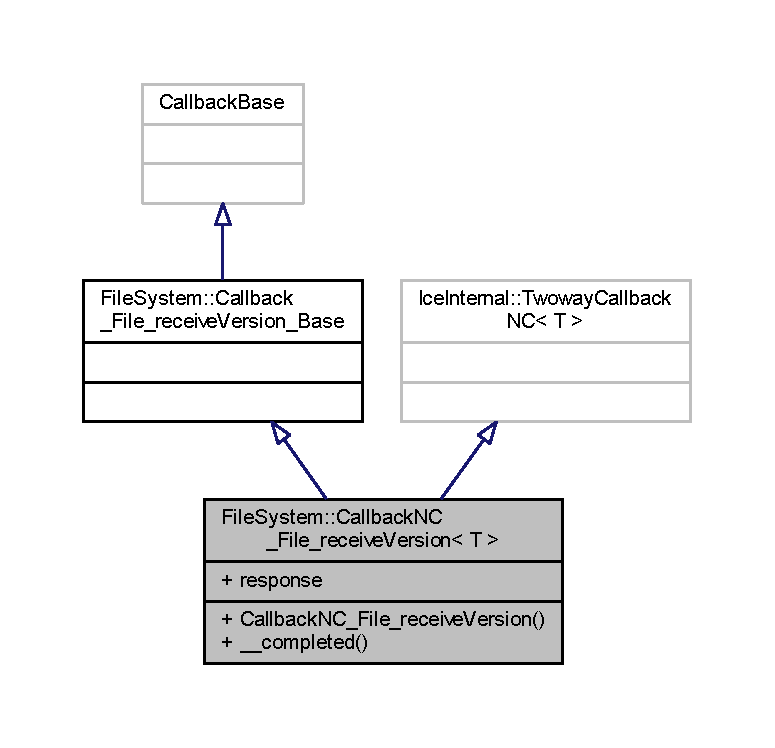
\includegraphics[width=350pt]{class_file_system_1_1_callback_n_c___file__receive_version__inherit__graph}
\end{center}
\end{figure}


Collaboration diagram for File\+System\+:\+:Callback\+N\+C\+\_\+\+File\+\_\+receive\+Version$<$ T $>$\+:
\nopagebreak
\begin{figure}[H]
\begin{center}
\leavevmode
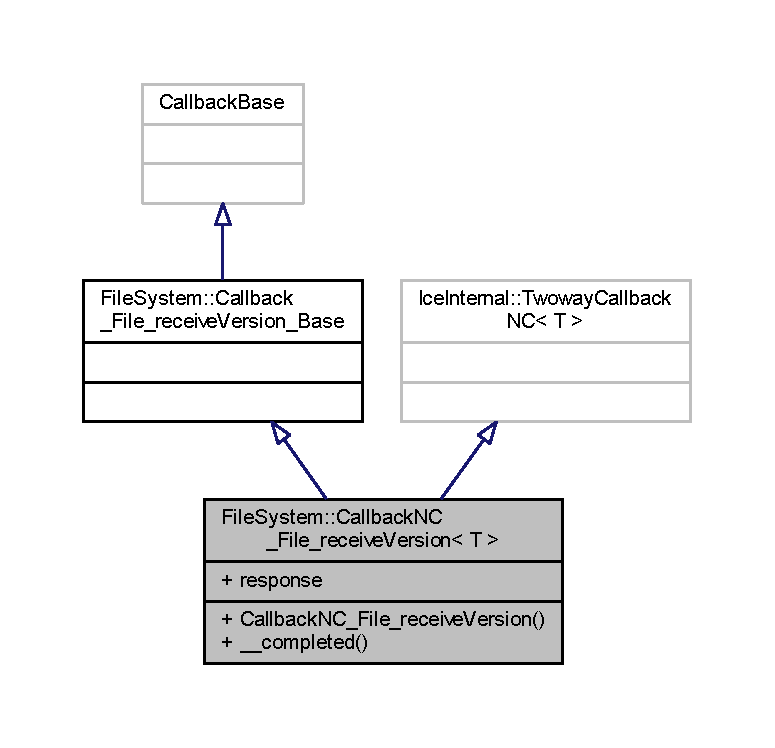
\includegraphics[width=350pt]{class_file_system_1_1_callback_n_c___file__receive_version__coll__graph}
\end{center}
\end{figure}
\subsection*{Public Types}
\begin{DoxyCompactItemize}
\item 
typedef Ice\+Util\+::\+Handle$<$ T $>$ \hyperlink{class_file_system_1_1_callback_n_c___file__receive_version_a4bb40a1c1a5f5407c5c42bf0ee950065}{T\+Ptr}
\item 
typedef void(T\+::$\ast$ \hyperlink{class_file_system_1_1_callback_n_c___file__receive_version_a852c42ee48702dc3f7fe6c0301755500}{Exception}) (const \+::Ice\+::\+Exception \&)
\item 
typedef void(T\+::$\ast$ \hyperlink{class_file_system_1_1_callback_n_c___file__receive_version_ab1b34ba3456b31c2a30649702a73c7a6}{Sent}) (bool)
\item 
typedef void(T\+::$\ast$ \hyperlink{class_file_system_1_1_callback_n_c___file__receive_version_aa60cb3d411660e0c5d1c38f3d2fd6977}{Response}) (const \+::\hyperlink{namespace_file_system_a5c85de065f9c451ae1d1dea2dacb68c5}{File\+System\+::\+Byte\+Seq} \&)
\end{DoxyCompactItemize}
\subsection*{Public Member Functions}
\begin{DoxyCompactItemize}
\item 
\hyperlink{class_file_system_1_1_callback_n_c___file__receive_version_a352d4f6cace878c0e61db502466b8b6f}{Callback\+N\+C\+\_\+\+File\+\_\+receive\+Version} (const \hyperlink{class_file_system_1_1_callback_n_c___file__receive_version_a4bb40a1c1a5f5407c5c42bf0ee950065}{T\+Ptr} \&obj, \hyperlink{class_file_system_1_1_callback_n_c___file__receive_version_aa60cb3d411660e0c5d1c38f3d2fd6977}{Response} cb, \hyperlink{class_file_system_1_1_callback_n_c___file__receive_version_a852c42ee48702dc3f7fe6c0301755500}{Exception} excb, \hyperlink{class_file_system_1_1_callback_n_c___file__receive_version_ab1b34ba3456b31c2a30649702a73c7a6}{Sent} sentcb)
\item 
virtual void \hyperlink{class_file_system_1_1_callback_n_c___file__receive_version_aa9bfe6619d3b126de9478f76d674e0dd}{\+\_\+\+\_\+completed} (const \+::Ice\+::\+Async\+Result\+Ptr \&\+\_\+\+\_\+result) const 
\end{DoxyCompactItemize}
\subsection*{Public Attributes}
\begin{DoxyCompactItemize}
\item 
\hyperlink{class_file_system_1_1_callback_n_c___file__receive_version_aa60cb3d411660e0c5d1c38f3d2fd6977}{Response} \hyperlink{class_file_system_1_1_callback_n_c___file__receive_version_a6acc4146a98beaf8732a5a0836206c54}{response}
\end{DoxyCompactItemize}


\subsection{Member Typedef Documentation}
\hypertarget{class_file_system_1_1_callback_n_c___file__receive_version_a852c42ee48702dc3f7fe6c0301755500}{}\index{File\+System\+::\+Callback\+N\+C\+\_\+\+File\+\_\+receive\+Version@{File\+System\+::\+Callback\+N\+C\+\_\+\+File\+\_\+receive\+Version}!Exception@{Exception}}
\index{Exception@{Exception}!File\+System\+::\+Callback\+N\+C\+\_\+\+File\+\_\+receive\+Version@{File\+System\+::\+Callback\+N\+C\+\_\+\+File\+\_\+receive\+Version}}
\subsubsection[{Exception}]{\setlength{\rightskip}{0pt plus 5cm}template$<$class T$>$ typedef void(T\+::$\ast$ {\bf File\+System\+::\+Callback\+N\+C\+\_\+\+File\+\_\+receive\+Version}$<$ T $>$\+::Exception) (const \+::Ice\+::\+Exception \&)}\label{class_file_system_1_1_callback_n_c___file__receive_version_a852c42ee48702dc3f7fe6c0301755500}
\hypertarget{class_file_system_1_1_callback_n_c___file__receive_version_aa60cb3d411660e0c5d1c38f3d2fd6977}{}\index{File\+System\+::\+Callback\+N\+C\+\_\+\+File\+\_\+receive\+Version@{File\+System\+::\+Callback\+N\+C\+\_\+\+File\+\_\+receive\+Version}!Response@{Response}}
\index{Response@{Response}!File\+System\+::\+Callback\+N\+C\+\_\+\+File\+\_\+receive\+Version@{File\+System\+::\+Callback\+N\+C\+\_\+\+File\+\_\+receive\+Version}}
\subsubsection[{Response}]{\setlength{\rightskip}{0pt plus 5cm}template$<$class T$>$ typedef void(T\+::$\ast$ {\bf File\+System\+::\+Callback\+N\+C\+\_\+\+File\+\_\+receive\+Version}$<$ T $>$\+::Response) (const \+::{\bf File\+System\+::\+Byte\+Seq} \&)}\label{class_file_system_1_1_callback_n_c___file__receive_version_aa60cb3d411660e0c5d1c38f3d2fd6977}
\hypertarget{class_file_system_1_1_callback_n_c___file__receive_version_ab1b34ba3456b31c2a30649702a73c7a6}{}\index{File\+System\+::\+Callback\+N\+C\+\_\+\+File\+\_\+receive\+Version@{File\+System\+::\+Callback\+N\+C\+\_\+\+File\+\_\+receive\+Version}!Sent@{Sent}}
\index{Sent@{Sent}!File\+System\+::\+Callback\+N\+C\+\_\+\+File\+\_\+receive\+Version@{File\+System\+::\+Callback\+N\+C\+\_\+\+File\+\_\+receive\+Version}}
\subsubsection[{Sent}]{\setlength{\rightskip}{0pt plus 5cm}template$<$class T$>$ typedef void(T\+::$\ast$ {\bf File\+System\+::\+Callback\+N\+C\+\_\+\+File\+\_\+receive\+Version}$<$ T $>$\+::Sent) (bool)}\label{class_file_system_1_1_callback_n_c___file__receive_version_ab1b34ba3456b31c2a30649702a73c7a6}
\hypertarget{class_file_system_1_1_callback_n_c___file__receive_version_a4bb40a1c1a5f5407c5c42bf0ee950065}{}\index{File\+System\+::\+Callback\+N\+C\+\_\+\+File\+\_\+receive\+Version@{File\+System\+::\+Callback\+N\+C\+\_\+\+File\+\_\+receive\+Version}!T\+Ptr@{T\+Ptr}}
\index{T\+Ptr@{T\+Ptr}!File\+System\+::\+Callback\+N\+C\+\_\+\+File\+\_\+receive\+Version@{File\+System\+::\+Callback\+N\+C\+\_\+\+File\+\_\+receive\+Version}}
\subsubsection[{T\+Ptr}]{\setlength{\rightskip}{0pt plus 5cm}template$<$class T$>$ typedef Ice\+Util\+::\+Handle$<$T$>$ {\bf File\+System\+::\+Callback\+N\+C\+\_\+\+File\+\_\+receive\+Version}$<$ T $>$\+::{\bf T\+Ptr}}\label{class_file_system_1_1_callback_n_c___file__receive_version_a4bb40a1c1a5f5407c5c42bf0ee950065}


\subsection{Constructor \& Destructor Documentation}
\hypertarget{class_file_system_1_1_callback_n_c___file__receive_version_a352d4f6cace878c0e61db502466b8b6f}{}\index{File\+System\+::\+Callback\+N\+C\+\_\+\+File\+\_\+receive\+Version@{File\+System\+::\+Callback\+N\+C\+\_\+\+File\+\_\+receive\+Version}!Callback\+N\+C\+\_\+\+File\+\_\+receive\+Version@{Callback\+N\+C\+\_\+\+File\+\_\+receive\+Version}}
\index{Callback\+N\+C\+\_\+\+File\+\_\+receive\+Version@{Callback\+N\+C\+\_\+\+File\+\_\+receive\+Version}!File\+System\+::\+Callback\+N\+C\+\_\+\+File\+\_\+receive\+Version@{File\+System\+::\+Callback\+N\+C\+\_\+\+File\+\_\+receive\+Version}}
\subsubsection[{Callback\+N\+C\+\_\+\+File\+\_\+receive\+Version}]{\setlength{\rightskip}{0pt plus 5cm}template$<$class T$>$ {\bf File\+System\+::\+Callback\+N\+C\+\_\+\+File\+\_\+receive\+Version}$<$ T $>$\+::{\bf Callback\+N\+C\+\_\+\+File\+\_\+receive\+Version} (
\begin{DoxyParamCaption}
\item[{const {\bf T\+Ptr} \&}]{obj, }
\item[{{\bf Response}}]{cb, }
\item[{{\bf Exception}}]{excb, }
\item[{{\bf Sent}}]{sentcb}
\end{DoxyParamCaption}
)\hspace{0.3cm}{\ttfamily [inline]}}\label{class_file_system_1_1_callback_n_c___file__receive_version_a352d4f6cace878c0e61db502466b8b6f}


\subsection{Member Function Documentation}
\hypertarget{class_file_system_1_1_callback_n_c___file__receive_version_aa9bfe6619d3b126de9478f76d674e0dd}{}\index{File\+System\+::\+Callback\+N\+C\+\_\+\+File\+\_\+receive\+Version@{File\+System\+::\+Callback\+N\+C\+\_\+\+File\+\_\+receive\+Version}!\+\_\+\+\_\+completed@{\+\_\+\+\_\+completed}}
\index{\+\_\+\+\_\+completed@{\+\_\+\+\_\+completed}!File\+System\+::\+Callback\+N\+C\+\_\+\+File\+\_\+receive\+Version@{File\+System\+::\+Callback\+N\+C\+\_\+\+File\+\_\+receive\+Version}}
\subsubsection[{\+\_\+\+\_\+completed}]{\setlength{\rightskip}{0pt plus 5cm}template$<$class T$>$ virtual void {\bf File\+System\+::\+Callback\+N\+C\+\_\+\+File\+\_\+receive\+Version}$<$ T $>$\+::\+\_\+\+\_\+completed (
\begin{DoxyParamCaption}
\item[{const \+::Ice\+::\+Async\+Result\+Ptr \&}]{\+\_\+\+\_\+result}
\end{DoxyParamCaption}
) const\hspace{0.3cm}{\ttfamily [inline]}, {\ttfamily [virtual]}}\label{class_file_system_1_1_callback_n_c___file__receive_version_aa9bfe6619d3b126de9478f76d674e0dd}


\subsection{Member Data Documentation}
\hypertarget{class_file_system_1_1_callback_n_c___file__receive_version_a6acc4146a98beaf8732a5a0836206c54}{}\index{File\+System\+::\+Callback\+N\+C\+\_\+\+File\+\_\+receive\+Version@{File\+System\+::\+Callback\+N\+C\+\_\+\+File\+\_\+receive\+Version}!response@{response}}
\index{response@{response}!File\+System\+::\+Callback\+N\+C\+\_\+\+File\+\_\+receive\+Version@{File\+System\+::\+Callback\+N\+C\+\_\+\+File\+\_\+receive\+Version}}
\subsubsection[{response}]{\setlength{\rightskip}{0pt plus 5cm}template$<$class T$>$ {\bf Response} {\bf File\+System\+::\+Callback\+N\+C\+\_\+\+File\+\_\+receive\+Version}$<$ T $>$\+::response}\label{class_file_system_1_1_callback_n_c___file__receive_version_a6acc4146a98beaf8732a5a0836206c54}


The documentation for this class was generated from the following file\+:\begin{DoxyCompactItemize}
\item 
\hyperlink{_file_system_8h}{File\+System.\+h}\end{DoxyCompactItemize}

\hypertarget{class_file_system_1_1_callback_n_c___file__send_file}{}\section{File\+System\+:\+:Callback\+N\+C\+\_\+\+File\+\_\+send\+File$<$ T $>$ Class Template Reference}
\label{class_file_system_1_1_callback_n_c___file__send_file}\index{File\+System\+::\+Callback\+N\+C\+\_\+\+File\+\_\+send\+File$<$ T $>$@{File\+System\+::\+Callback\+N\+C\+\_\+\+File\+\_\+send\+File$<$ T $>$}}


{\ttfamily \#include $<$File\+System.\+h$>$}



Inheritance diagram for File\+System\+:\+:Callback\+N\+C\+\_\+\+File\+\_\+send\+File$<$ T $>$\+:
\nopagebreak
\begin{figure}[H]
\begin{center}
\leavevmode
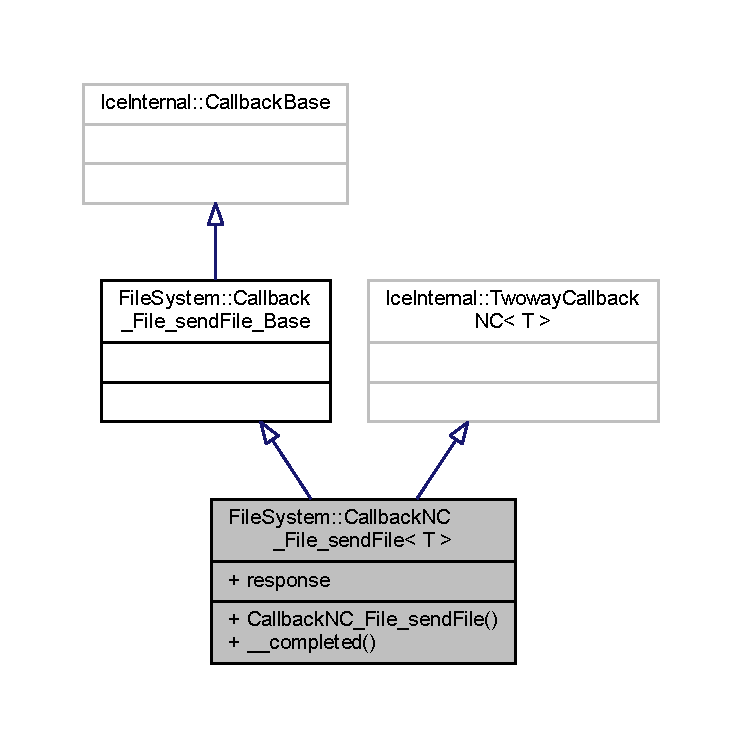
\includegraphics[width=350pt]{class_file_system_1_1_callback_n_c___file__send_file__inherit__graph}
\end{center}
\end{figure}


Collaboration diagram for File\+System\+:\+:Callback\+N\+C\+\_\+\+File\+\_\+send\+File$<$ T $>$\+:
\nopagebreak
\begin{figure}[H]
\begin{center}
\leavevmode
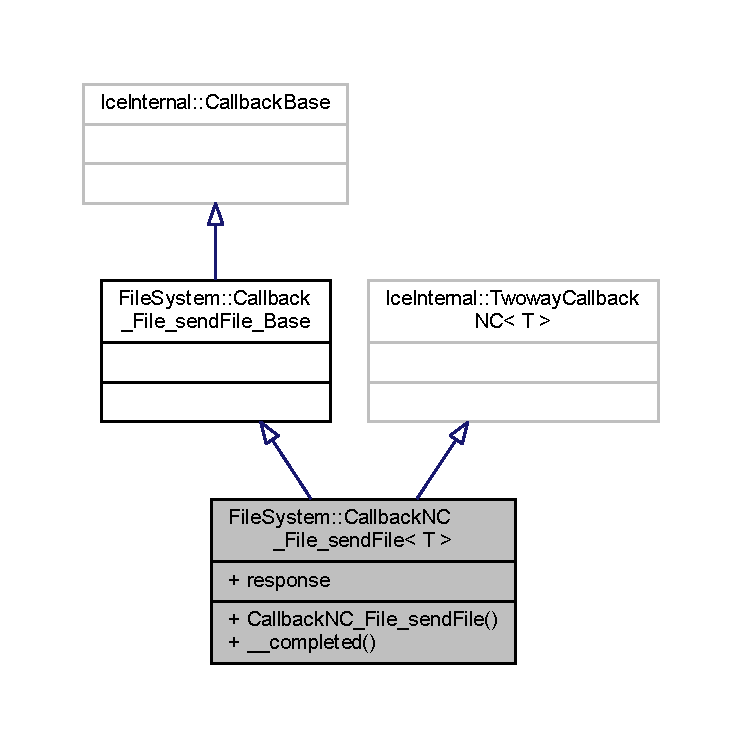
\includegraphics[width=350pt]{class_file_system_1_1_callback_n_c___file__send_file__coll__graph}
\end{center}
\end{figure}
\subsection*{Public Types}
\begin{DoxyCompactItemize}
\item 
typedef Ice\+Util\+::\+Handle$<$ T $>$ \hyperlink{class_file_system_1_1_callback_n_c___file__send_file_a0b4de40be68e6670f4d7d887127adfa1}{T\+Ptr}
\item 
typedef void(T\+::$\ast$ \hyperlink{class_file_system_1_1_callback_n_c___file__send_file_a6b3e46d31e2767255629f84dbdc41de1}{Exception}) (const \+::Ice\+::\+Exception \&)
\item 
typedef void(T\+::$\ast$ \hyperlink{class_file_system_1_1_callback_n_c___file__send_file_a64d311bef39e6c24f7294a62ac449373}{Sent}) (bool)
\item 
typedef void(T\+::$\ast$ \hyperlink{class_file_system_1_1_callback_n_c___file__send_file_ac2f2e02236bc1e7302a100c796b9d881}{Response}) (bool)
\end{DoxyCompactItemize}
\subsection*{Public Member Functions}
\begin{DoxyCompactItemize}
\item 
\hyperlink{class_file_system_1_1_callback_n_c___file__send_file_aa900895a968072ca878825b7238a0993}{Callback\+N\+C\+\_\+\+File\+\_\+send\+File} (const \hyperlink{class_file_system_1_1_callback_n_c___file__send_file_a0b4de40be68e6670f4d7d887127adfa1}{T\+Ptr} \&obj, \hyperlink{class_file_system_1_1_callback_n_c___file__send_file_ac2f2e02236bc1e7302a100c796b9d881}{Response} cb, \hyperlink{class_file_system_1_1_callback_n_c___file__send_file_a6b3e46d31e2767255629f84dbdc41de1}{Exception} excb, \hyperlink{class_file_system_1_1_callback_n_c___file__send_file_a64d311bef39e6c24f7294a62ac449373}{Sent} sentcb)
\item 
virtual void \hyperlink{class_file_system_1_1_callback_n_c___file__send_file_a7298a6e4457c053513bdd5320b868980}{\+\_\+\+\_\+completed} (const \+::Ice\+::\+Async\+Result\+Ptr \&\+\_\+\+\_\+result) const 
\end{DoxyCompactItemize}
\subsection*{Public Attributes}
\begin{DoxyCompactItemize}
\item 
\hyperlink{class_file_system_1_1_callback_n_c___file__send_file_ac2f2e02236bc1e7302a100c796b9d881}{Response} \hyperlink{class_file_system_1_1_callback_n_c___file__send_file_a162fe4aa10743079f5dcc3afce72467d}{response}
\end{DoxyCompactItemize}


\subsection{Member Typedef Documentation}
\hypertarget{class_file_system_1_1_callback_n_c___file__send_file_a6b3e46d31e2767255629f84dbdc41de1}{}\index{File\+System\+::\+Callback\+N\+C\+\_\+\+File\+\_\+send\+File@{File\+System\+::\+Callback\+N\+C\+\_\+\+File\+\_\+send\+File}!Exception@{Exception}}
\index{Exception@{Exception}!File\+System\+::\+Callback\+N\+C\+\_\+\+File\+\_\+send\+File@{File\+System\+::\+Callback\+N\+C\+\_\+\+File\+\_\+send\+File}}
\subsubsection[{Exception}]{\setlength{\rightskip}{0pt plus 5cm}template$<$class T$>$ typedef void(T\+::$\ast$ {\bf File\+System\+::\+Callback\+N\+C\+\_\+\+File\+\_\+send\+File}$<$ T $>$\+::Exception) (const \+::Ice\+::\+Exception \&)}\label{class_file_system_1_1_callback_n_c___file__send_file_a6b3e46d31e2767255629f84dbdc41de1}
\hypertarget{class_file_system_1_1_callback_n_c___file__send_file_ac2f2e02236bc1e7302a100c796b9d881}{}\index{File\+System\+::\+Callback\+N\+C\+\_\+\+File\+\_\+send\+File@{File\+System\+::\+Callback\+N\+C\+\_\+\+File\+\_\+send\+File}!Response@{Response}}
\index{Response@{Response}!File\+System\+::\+Callback\+N\+C\+\_\+\+File\+\_\+send\+File@{File\+System\+::\+Callback\+N\+C\+\_\+\+File\+\_\+send\+File}}
\subsubsection[{Response}]{\setlength{\rightskip}{0pt plus 5cm}template$<$class T$>$ typedef void(T\+::$\ast$ {\bf File\+System\+::\+Callback\+N\+C\+\_\+\+File\+\_\+send\+File}$<$ T $>$\+::Response) (bool)}\label{class_file_system_1_1_callback_n_c___file__send_file_ac2f2e02236bc1e7302a100c796b9d881}
\hypertarget{class_file_system_1_1_callback_n_c___file__send_file_a64d311bef39e6c24f7294a62ac449373}{}\index{File\+System\+::\+Callback\+N\+C\+\_\+\+File\+\_\+send\+File@{File\+System\+::\+Callback\+N\+C\+\_\+\+File\+\_\+send\+File}!Sent@{Sent}}
\index{Sent@{Sent}!File\+System\+::\+Callback\+N\+C\+\_\+\+File\+\_\+send\+File@{File\+System\+::\+Callback\+N\+C\+\_\+\+File\+\_\+send\+File}}
\subsubsection[{Sent}]{\setlength{\rightskip}{0pt plus 5cm}template$<$class T$>$ typedef void(T\+::$\ast$ {\bf File\+System\+::\+Callback\+N\+C\+\_\+\+File\+\_\+send\+File}$<$ T $>$\+::Sent) (bool)}\label{class_file_system_1_1_callback_n_c___file__send_file_a64d311bef39e6c24f7294a62ac449373}
\hypertarget{class_file_system_1_1_callback_n_c___file__send_file_a0b4de40be68e6670f4d7d887127adfa1}{}\index{File\+System\+::\+Callback\+N\+C\+\_\+\+File\+\_\+send\+File@{File\+System\+::\+Callback\+N\+C\+\_\+\+File\+\_\+send\+File}!T\+Ptr@{T\+Ptr}}
\index{T\+Ptr@{T\+Ptr}!File\+System\+::\+Callback\+N\+C\+\_\+\+File\+\_\+send\+File@{File\+System\+::\+Callback\+N\+C\+\_\+\+File\+\_\+send\+File}}
\subsubsection[{T\+Ptr}]{\setlength{\rightskip}{0pt plus 5cm}template$<$class T$>$ typedef Ice\+Util\+::\+Handle$<$T$>$ {\bf File\+System\+::\+Callback\+N\+C\+\_\+\+File\+\_\+send\+File}$<$ T $>$\+::{\bf T\+Ptr}}\label{class_file_system_1_1_callback_n_c___file__send_file_a0b4de40be68e6670f4d7d887127adfa1}


\subsection{Constructor \& Destructor Documentation}
\hypertarget{class_file_system_1_1_callback_n_c___file__send_file_aa900895a968072ca878825b7238a0993}{}\index{File\+System\+::\+Callback\+N\+C\+\_\+\+File\+\_\+send\+File@{File\+System\+::\+Callback\+N\+C\+\_\+\+File\+\_\+send\+File}!Callback\+N\+C\+\_\+\+File\+\_\+send\+File@{Callback\+N\+C\+\_\+\+File\+\_\+send\+File}}
\index{Callback\+N\+C\+\_\+\+File\+\_\+send\+File@{Callback\+N\+C\+\_\+\+File\+\_\+send\+File}!File\+System\+::\+Callback\+N\+C\+\_\+\+File\+\_\+send\+File@{File\+System\+::\+Callback\+N\+C\+\_\+\+File\+\_\+send\+File}}
\subsubsection[{Callback\+N\+C\+\_\+\+File\+\_\+send\+File}]{\setlength{\rightskip}{0pt plus 5cm}template$<$class T$>$ {\bf File\+System\+::\+Callback\+N\+C\+\_\+\+File\+\_\+send\+File}$<$ T $>$\+::{\bf Callback\+N\+C\+\_\+\+File\+\_\+send\+File} (
\begin{DoxyParamCaption}
\item[{const {\bf T\+Ptr} \&}]{obj, }
\item[{{\bf Response}}]{cb, }
\item[{{\bf Exception}}]{excb, }
\item[{{\bf Sent}}]{sentcb}
\end{DoxyParamCaption}
)\hspace{0.3cm}{\ttfamily [inline]}}\label{class_file_system_1_1_callback_n_c___file__send_file_aa900895a968072ca878825b7238a0993}


\subsection{Member Function Documentation}
\hypertarget{class_file_system_1_1_callback_n_c___file__send_file_a7298a6e4457c053513bdd5320b868980}{}\index{File\+System\+::\+Callback\+N\+C\+\_\+\+File\+\_\+send\+File@{File\+System\+::\+Callback\+N\+C\+\_\+\+File\+\_\+send\+File}!\+\_\+\+\_\+completed@{\+\_\+\+\_\+completed}}
\index{\+\_\+\+\_\+completed@{\+\_\+\+\_\+completed}!File\+System\+::\+Callback\+N\+C\+\_\+\+File\+\_\+send\+File@{File\+System\+::\+Callback\+N\+C\+\_\+\+File\+\_\+send\+File}}
\subsubsection[{\+\_\+\+\_\+completed}]{\setlength{\rightskip}{0pt plus 5cm}template$<$class T$>$ virtual void {\bf File\+System\+::\+Callback\+N\+C\+\_\+\+File\+\_\+send\+File}$<$ T $>$\+::\+\_\+\+\_\+completed (
\begin{DoxyParamCaption}
\item[{const \+::Ice\+::\+Async\+Result\+Ptr \&}]{\+\_\+\+\_\+result}
\end{DoxyParamCaption}
) const\hspace{0.3cm}{\ttfamily [inline]}, {\ttfamily [virtual]}}\label{class_file_system_1_1_callback_n_c___file__send_file_a7298a6e4457c053513bdd5320b868980}


\subsection{Member Data Documentation}
\hypertarget{class_file_system_1_1_callback_n_c___file__send_file_a162fe4aa10743079f5dcc3afce72467d}{}\index{File\+System\+::\+Callback\+N\+C\+\_\+\+File\+\_\+send\+File@{File\+System\+::\+Callback\+N\+C\+\_\+\+File\+\_\+send\+File}!response@{response}}
\index{response@{response}!File\+System\+::\+Callback\+N\+C\+\_\+\+File\+\_\+send\+File@{File\+System\+::\+Callback\+N\+C\+\_\+\+File\+\_\+send\+File}}
\subsubsection[{response}]{\setlength{\rightskip}{0pt plus 5cm}template$<$class T$>$ {\bf Response} {\bf File\+System\+::\+Callback\+N\+C\+\_\+\+File\+\_\+send\+File}$<$ T $>$\+::response}\label{class_file_system_1_1_callback_n_c___file__send_file_a162fe4aa10743079f5dcc3afce72467d}


The documentation for this class was generated from the following file\+:\begin{DoxyCompactItemize}
\item 
\hyperlink{_file_system_8h}{File\+System.\+h}\end{DoxyCompactItemize}

\hypertarget{class_ice_proxy_1_1_file_system_1_1_file}{}\section{Ice\+Proxy\+:\+:File\+System\+:\+:File Class Reference}
\label{class_ice_proxy_1_1_file_system_1_1_file}\index{Ice\+Proxy\+::\+File\+System\+::\+File@{Ice\+Proxy\+::\+File\+System\+::\+File}}


{\ttfamily \#include $<$File\+System.\+h$>$}



Inheritance diagram for Ice\+Proxy\+:\+:File\+System\+:\+:File\+:
\nopagebreak
\begin{figure}[H]
\begin{center}
\leavevmode
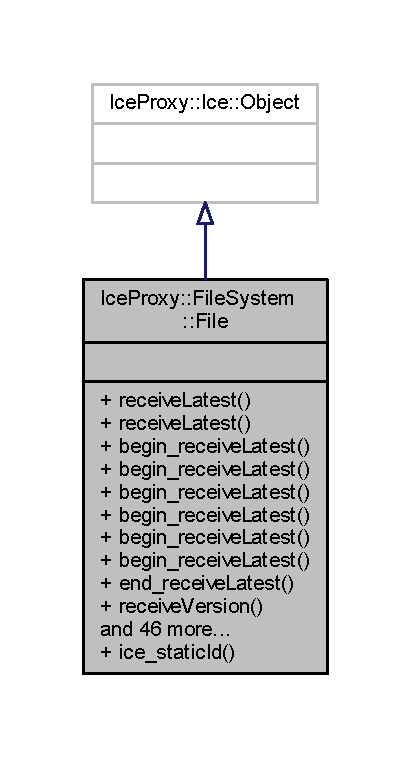
\includegraphics[width=197pt]{class_ice_proxy_1_1_file_system_1_1_file__inherit__graph}
\end{center}
\end{figure}


Collaboration diagram for Ice\+Proxy\+:\+:File\+System\+:\+:File\+:
\nopagebreak
\begin{figure}[H]
\begin{center}
\leavevmode
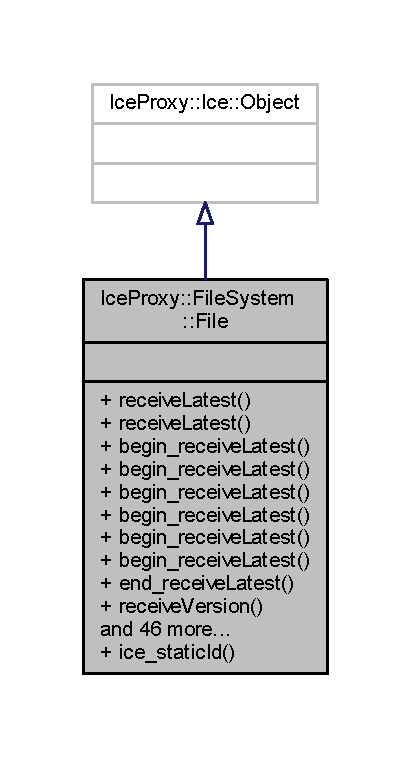
\includegraphics[width=197pt]{class_ice_proxy_1_1_file_system_1_1_file__coll__graph}
\end{center}
\end{figure}
\subsection*{Public Member Functions}
\begin{DoxyCompactItemize}
\item 
\+::\hyperlink{namespace_file_system_a5c85de065f9c451ae1d1dea2dacb68c5}{File\+System\+::\+Byte\+Seq} \hyperlink{class_ice_proxy_1_1_file_system_1_1_file_aa235edc359a9e7cd57aadd063078c48c}{receive\+Latest} (const \+::std\+::string \&sec, const \+::std\+::string \&art, const \+::std\+::string \&type, const \+::std\+::string \&f\+Name)
\item 
\+::\hyperlink{namespace_file_system_a5c85de065f9c451ae1d1dea2dacb68c5}{File\+System\+::\+Byte\+Seq} \hyperlink{class_ice_proxy_1_1_file_system_1_1_file_a03bd9459852dd73aa6d9945160a7dc81}{receive\+Latest} (const \+::std\+::string \&sec, const \+::std\+::string \&art, const \+::std\+::string \&type, const \+::std\+::string \&f\+Name, const \+::Ice\+::\+Context \&\+\_\+\+\_\+ctx)
\item 
\+::Ice\+::\+Async\+Result\+Ptr \hyperlink{class_ice_proxy_1_1_file_system_1_1_file_ab0bfc4cf2f256f81a0b7b0fe9bb09b94}{begin\+\_\+receive\+Latest} (const \+::std\+::string \&sec, const \+::std\+::string \&art, const \+::std\+::string \&type, const \+::std\+::string \&f\+Name)
\item 
\+::Ice\+::\+Async\+Result\+Ptr \hyperlink{class_ice_proxy_1_1_file_system_1_1_file_a30a10d0bcea0de70b3f9c47ed5e91b2b}{begin\+\_\+receive\+Latest} (const \+::std\+::string \&sec, const \+::std\+::string \&art, const \+::std\+::string \&type, const \+::std\+::string \&f\+Name, const \+::Ice\+::\+Context \&\+\_\+\+\_\+ctx)
\item 
\+::Ice\+::\+Async\+Result\+Ptr \hyperlink{class_ice_proxy_1_1_file_system_1_1_file_a3037db699157ab957468c3a77afca147}{begin\+\_\+receive\+Latest} (const \+::std\+::string \&sec, const \+::std\+::string \&art, const \+::std\+::string \&type, const \+::std\+::string \&f\+Name, const \+::Ice\+::\+Callback\+Ptr \&\+\_\+\+\_\+del, const \+::Ice\+::\+Local\+Object\+Ptr \&\+\_\+\+\_\+cookie=0)
\item 
\+::Ice\+::\+Async\+Result\+Ptr \hyperlink{class_ice_proxy_1_1_file_system_1_1_file_a2a122da9b3a0d5e3191017c4b0f28390}{begin\+\_\+receive\+Latest} (const \+::std\+::string \&sec, const \+::std\+::string \&art, const \+::std\+::string \&type, const \+::std\+::string \&f\+Name, const \+::Ice\+::\+Context \&\+\_\+\+\_\+ctx, const \+::Ice\+::\+Callback\+Ptr \&\+\_\+\+\_\+del, const \+::Ice\+::\+Local\+Object\+Ptr \&\+\_\+\+\_\+cookie=0)
\item 
\+::Ice\+::\+Async\+Result\+Ptr \hyperlink{class_ice_proxy_1_1_file_system_1_1_file_a1367692f927b1a40d2a338efc588f4ff}{begin\+\_\+receive\+Latest} (const \+::std\+::string \&sec, const \+::std\+::string \&art, const \+::std\+::string \&type, const \+::std\+::string \&f\+Name, const \+::\hyperlink{namespace_file_system_a86fe38e325e02ddd26f665f486d51837}{File\+System\+::\+Callback\+\_\+\+File\+\_\+receive\+Latest\+Ptr} \&\+\_\+\+\_\+del, const \+::Ice\+::\+Local\+Object\+Ptr \&\+\_\+\+\_\+cookie=0)
\item 
\+::Ice\+::\+Async\+Result\+Ptr \hyperlink{class_ice_proxy_1_1_file_system_1_1_file_ad8d75389e9e2115727c65b92f8a09b27}{begin\+\_\+receive\+Latest} (const \+::std\+::string \&sec, const \+::std\+::string \&art, const \+::std\+::string \&type, const \+::std\+::string \&f\+Name, const \+::Ice\+::\+Context \&\+\_\+\+\_\+ctx, const \+::\hyperlink{namespace_file_system_a86fe38e325e02ddd26f665f486d51837}{File\+System\+::\+Callback\+\_\+\+File\+\_\+receive\+Latest\+Ptr} \&\+\_\+\+\_\+del, const \+::Ice\+::\+Local\+Object\+Ptr \&\+\_\+\+\_\+cookie=0)
\item 
\+::\hyperlink{namespace_file_system_a5c85de065f9c451ae1d1dea2dacb68c5}{File\+System\+::\+Byte\+Seq} \hyperlink{class_ice_proxy_1_1_file_system_1_1_file_a4993bd781a99fe53e71bef94a752f543}{end\+\_\+receive\+Latest} (const \+::Ice\+::\+Async\+Result\+Ptr \&)
\item 
\+::\hyperlink{namespace_file_system_a5c85de065f9c451ae1d1dea2dacb68c5}{File\+System\+::\+Byte\+Seq} \hyperlink{class_ice_proxy_1_1_file_system_1_1_file_aef65d4fa3028c32e712162aea839f4f6}{receive\+Version} (const \+::std\+::string \&sec, const \+::std\+::string \&art, const \+::std\+::string \&type, const \+::std\+::string \&f\+Name,\+::Ice\+::\+Int ver)
\item 
\+::\hyperlink{namespace_file_system_a5c85de065f9c451ae1d1dea2dacb68c5}{File\+System\+::\+Byte\+Seq} \hyperlink{class_ice_proxy_1_1_file_system_1_1_file_af1ea34ee0b4b9579e684c363f1826243}{receive\+Version} (const \+::std\+::string \&sec, const \+::std\+::string \&art, const \+::std\+::string \&type, const \+::std\+::string \&f\+Name,\+::Ice\+::\+Int ver, const \+::Ice\+::\+Context \&\+\_\+\+\_\+ctx)
\item 
\+::Ice\+::\+Async\+Result\+Ptr \hyperlink{class_ice_proxy_1_1_file_system_1_1_file_a4f6e2f8b3fbb888b74ed6e40d1da51b3}{begin\+\_\+receive\+Version} (const \+::std\+::string \&sec, const \+::std\+::string \&art, const \+::std\+::string \&type, const \+::std\+::string \&f\+Name,\+::Ice\+::\+Int ver)
\item 
\+::Ice\+::\+Async\+Result\+Ptr \hyperlink{class_ice_proxy_1_1_file_system_1_1_file_ac031ccd296c05c2fa3d35ffb5bd5567a}{begin\+\_\+receive\+Version} (const \+::std\+::string \&sec, const \+::std\+::string \&art, const \+::std\+::string \&type, const \+::std\+::string \&f\+Name,\+::Ice\+::\+Int ver, const \+::Ice\+::\+Context \&\+\_\+\+\_\+ctx)
\item 
\+::Ice\+::\+Async\+Result\+Ptr \hyperlink{class_ice_proxy_1_1_file_system_1_1_file_a018221725b3a59eece1dc97ae731ebe3}{begin\+\_\+receive\+Version} (const \+::std\+::string \&sec, const \+::std\+::string \&art, const \+::std\+::string \&type, const \+::std\+::string \&f\+Name,\+::Ice\+::\+Int ver, const \+::Ice\+::\+Callback\+Ptr \&\+\_\+\+\_\+del, const \+::Ice\+::\+Local\+Object\+Ptr \&\+\_\+\+\_\+cookie=0)
\item 
\+::Ice\+::\+Async\+Result\+Ptr \hyperlink{class_ice_proxy_1_1_file_system_1_1_file_aa6b45e4cae6983ae197b639d7bd46b56}{begin\+\_\+receive\+Version} (const \+::std\+::string \&sec, const \+::std\+::string \&art, const \+::std\+::string \&type, const \+::std\+::string \&f\+Name,\+::Ice\+::\+Int ver, const \+::Ice\+::\+Context \&\+\_\+\+\_\+ctx, const \+::Ice\+::\+Callback\+Ptr \&\+\_\+\+\_\+del, const \+::Ice\+::\+Local\+Object\+Ptr \&\+\_\+\+\_\+cookie=0)
\item 
\+::Ice\+::\+Async\+Result\+Ptr \hyperlink{class_ice_proxy_1_1_file_system_1_1_file_a27ec313b8e57803b7659963738ad2946}{begin\+\_\+receive\+Version} (const \+::std\+::string \&sec, const \+::std\+::string \&art, const \+::std\+::string \&type, const \+::std\+::string \&f\+Name,\+::Ice\+::\+Int ver, const \+::\hyperlink{namespace_file_system_a9f139d463637347415d1d3dadefe9bad}{File\+System\+::\+Callback\+\_\+\+File\+\_\+receive\+Version\+Ptr} \&\+\_\+\+\_\+del, const \+::Ice\+::\+Local\+Object\+Ptr \&\+\_\+\+\_\+cookie=0)
\item 
\+::Ice\+::\+Async\+Result\+Ptr \hyperlink{class_ice_proxy_1_1_file_system_1_1_file_a160bd20bd4efbbcc3ba9644d072110bd}{begin\+\_\+receive\+Version} (const \+::std\+::string \&sec, const \+::std\+::string \&art, const \+::std\+::string \&type, const \+::std\+::string \&f\+Name,\+::Ice\+::\+Int ver, const \+::Ice\+::\+Context \&\+\_\+\+\_\+ctx, const \+::\hyperlink{namespace_file_system_a9f139d463637347415d1d3dadefe9bad}{File\+System\+::\+Callback\+\_\+\+File\+\_\+receive\+Version\+Ptr} \&\+\_\+\+\_\+del, const \+::Ice\+::\+Local\+Object\+Ptr \&\+\_\+\+\_\+cookie=0)
\item 
\+::\hyperlink{namespace_file_system_a5c85de065f9c451ae1d1dea2dacb68c5}{File\+System\+::\+Byte\+Seq} \hyperlink{class_ice_proxy_1_1_file_system_1_1_file_ab70bdc2bd55ab5af5c6c526e20b6073d}{end\+\_\+receive\+Version} (const \+::Ice\+::\+Async\+Result\+Ptr \&)
\item 
bool \hyperlink{class_ice_proxy_1_1_file_system_1_1_file_ab3708aa9ebb1399ce32a9507d925215d}{send\+File} (const \+::std\+::string \&sec, const \+::std\+::string \&art, const \+::std\+::string \&type, const \+::std\+::string \&f\+Name\+Ext, const \+::\hyperlink{namespace_file_system_a5c85de065f9c451ae1d1dea2dacb68c5}{File\+System\+::\+Byte\+Seq} \&seq)
\item 
bool \hyperlink{class_ice_proxy_1_1_file_system_1_1_file_a8d7b147b0f1542786a5be6e6c9f0d45a}{send\+File} (const \+::std\+::string \&sec, const \+::std\+::string \&art, const \+::std\+::string \&type, const \+::std\+::string \&f\+Name\+Ext, const \+::\hyperlink{namespace_file_system_a5c85de065f9c451ae1d1dea2dacb68c5}{File\+System\+::\+Byte\+Seq} \&seq, const \+::Ice\+::\+Context \&\+\_\+\+\_\+ctx)
\item 
\+::Ice\+::\+Async\+Result\+Ptr \hyperlink{class_ice_proxy_1_1_file_system_1_1_file_a713d1ca52a1c93ea3f2a6d8a26db6e83}{begin\+\_\+send\+File} (const \+::std\+::string \&sec, const \+::std\+::string \&art, const \+::std\+::string \&type, const \+::std\+::string \&f\+Name\+Ext, const \+::\hyperlink{namespace_file_system_a5c85de065f9c451ae1d1dea2dacb68c5}{File\+System\+::\+Byte\+Seq} \&seq)
\item 
\+::Ice\+::\+Async\+Result\+Ptr \hyperlink{class_ice_proxy_1_1_file_system_1_1_file_aaa9a30cd6344bb689d0aee77984be5d0}{begin\+\_\+send\+File} (const \+::std\+::string \&sec, const \+::std\+::string \&art, const \+::std\+::string \&type, const \+::std\+::string \&f\+Name\+Ext, const \+::\hyperlink{namespace_file_system_a5c85de065f9c451ae1d1dea2dacb68c5}{File\+System\+::\+Byte\+Seq} \&seq, const \+::Ice\+::\+Context \&\+\_\+\+\_\+ctx)
\item 
\+::Ice\+::\+Async\+Result\+Ptr \hyperlink{class_ice_proxy_1_1_file_system_1_1_file_a041ae45fbe56672712fc96545dab9e3a}{begin\+\_\+send\+File} (const \+::std\+::string \&sec, const \+::std\+::string \&art, const \+::std\+::string \&type, const \+::std\+::string \&f\+Name\+Ext, const \+::\hyperlink{namespace_file_system_a5c85de065f9c451ae1d1dea2dacb68c5}{File\+System\+::\+Byte\+Seq} \&seq, const \+::Ice\+::\+Callback\+Ptr \&\+\_\+\+\_\+del, const \+::Ice\+::\+Local\+Object\+Ptr \&\+\_\+\+\_\+cookie=0)
\item 
\+::Ice\+::\+Async\+Result\+Ptr \hyperlink{class_ice_proxy_1_1_file_system_1_1_file_a3f52adcc4284d6c31f9d51e69259b4b0}{begin\+\_\+send\+File} (const \+::std\+::string \&sec, const \+::std\+::string \&art, const \+::std\+::string \&type, const \+::std\+::string \&f\+Name\+Ext, const \+::\hyperlink{namespace_file_system_a5c85de065f9c451ae1d1dea2dacb68c5}{File\+System\+::\+Byte\+Seq} \&seq, const \+::Ice\+::\+Context \&\+\_\+\+\_\+ctx, const \+::Ice\+::\+Callback\+Ptr \&\+\_\+\+\_\+del, const \+::Ice\+::\+Local\+Object\+Ptr \&\+\_\+\+\_\+cookie=0)
\item 
\+::Ice\+::\+Async\+Result\+Ptr \hyperlink{class_ice_proxy_1_1_file_system_1_1_file_a954ec3abdc5196ed1397c1c230be466c}{begin\+\_\+send\+File} (const \+::std\+::string \&sec, const \+::std\+::string \&art, const \+::std\+::string \&type, const \+::std\+::string \&f\+Name\+Ext, const \+::\hyperlink{namespace_file_system_a5c85de065f9c451ae1d1dea2dacb68c5}{File\+System\+::\+Byte\+Seq} \&seq, const \+::\hyperlink{namespace_file_system_aa10040959d9776f7f500f38a2567b56e}{File\+System\+::\+Callback\+\_\+\+File\+\_\+send\+File\+Ptr} \&\+\_\+\+\_\+del, const \+::Ice\+::\+Local\+Object\+Ptr \&\+\_\+\+\_\+cookie=0)
\item 
\+::Ice\+::\+Async\+Result\+Ptr \hyperlink{class_ice_proxy_1_1_file_system_1_1_file_af6424fc76be5433e6eb9de590309726b}{begin\+\_\+send\+File} (const \+::std\+::string \&sec, const \+::std\+::string \&art, const \+::std\+::string \&type, const \+::std\+::string \&f\+Name\+Ext, const \+::\hyperlink{namespace_file_system_a5c85de065f9c451ae1d1dea2dacb68c5}{File\+System\+::\+Byte\+Seq} \&seq, const \+::Ice\+::\+Context \&\+\_\+\+\_\+ctx, const \+::\hyperlink{namespace_file_system_aa10040959d9776f7f500f38a2567b56e}{File\+System\+::\+Callback\+\_\+\+File\+\_\+send\+File\+Ptr} \&\+\_\+\+\_\+del, const \+::Ice\+::\+Local\+Object\+Ptr \&\+\_\+\+\_\+cookie=0)
\item 
bool \hyperlink{class_ice_proxy_1_1_file_system_1_1_file_aa3ce8b0bcafb195f706ac79732566695}{end\+\_\+send\+File} (const \+::Ice\+::\+Async\+Result\+Ptr \&)
\item 
\+::\hyperlink{namespace_file_system_ac32dc1eb34c060160b52edc7c4e37d6e}{File\+System\+::\+Ver\+Seq} \hyperlink{class_ice_proxy_1_1_file_system_1_1_file_aa210a366a64a16ed7e4a484f9f4ee93f}{get\+History} (const \+::std\+::string \&sec, const \+::std\+::string \&art, const \+::std\+::string \&type, const \+::std\+::string \&f\+Name)
\item 
\+::\hyperlink{namespace_file_system_ac32dc1eb34c060160b52edc7c4e37d6e}{File\+System\+::\+Ver\+Seq} \hyperlink{class_ice_proxy_1_1_file_system_1_1_file_ac5c5072e4bd9b5524178af3c5f4dfec6}{get\+History} (const \+::std\+::string \&sec, const \+::std\+::string \&art, const \+::std\+::string \&type, const \+::std\+::string \&f\+Name, const \+::Ice\+::\+Context \&\+\_\+\+\_\+ctx)
\item 
\+::Ice\+::\+Async\+Result\+Ptr \hyperlink{class_ice_proxy_1_1_file_system_1_1_file_a3f3e75a2fe26435cf701d5baaaad95bd}{begin\+\_\+get\+History} (const \+::std\+::string \&sec, const \+::std\+::string \&art, const \+::std\+::string \&type, const \+::std\+::string \&f\+Name)
\item 
\+::Ice\+::\+Async\+Result\+Ptr \hyperlink{class_ice_proxy_1_1_file_system_1_1_file_a04ac2d68187770df1ea1a219d8203f11}{begin\+\_\+get\+History} (const \+::std\+::string \&sec, const \+::std\+::string \&art, const \+::std\+::string \&type, const \+::std\+::string \&f\+Name, const \+::Ice\+::\+Context \&\+\_\+\+\_\+ctx)
\item 
\+::Ice\+::\+Async\+Result\+Ptr \hyperlink{class_ice_proxy_1_1_file_system_1_1_file_a11f334f03b1ed2d23106d1856081895e}{begin\+\_\+get\+History} (const \+::std\+::string \&sec, const \+::std\+::string \&art, const \+::std\+::string \&type, const \+::std\+::string \&f\+Name, const \+::Ice\+::\+Callback\+Ptr \&\+\_\+\+\_\+del, const \+::Ice\+::\+Local\+Object\+Ptr \&\+\_\+\+\_\+cookie=0)
\item 
\+::Ice\+::\+Async\+Result\+Ptr \hyperlink{class_ice_proxy_1_1_file_system_1_1_file_af44984d072cd39c97ca20e4915ec6248}{begin\+\_\+get\+History} (const \+::std\+::string \&sec, const \+::std\+::string \&art, const \+::std\+::string \&type, const \+::std\+::string \&f\+Name, const \+::Ice\+::\+Context \&\+\_\+\+\_\+ctx, const \+::Ice\+::\+Callback\+Ptr \&\+\_\+\+\_\+del, const \+::Ice\+::\+Local\+Object\+Ptr \&\+\_\+\+\_\+cookie=0)
\item 
\+::Ice\+::\+Async\+Result\+Ptr \hyperlink{class_ice_proxy_1_1_file_system_1_1_file_a34d25ea7db626c9c2629908e5c78c814}{begin\+\_\+get\+History} (const \+::std\+::string \&sec, const \+::std\+::string \&art, const \+::std\+::string \&type, const \+::std\+::string \&f\+Name, const \+::\hyperlink{namespace_file_system_a9dca00d90979e9c64452fc4123feed8e}{File\+System\+::\+Callback\+\_\+\+File\+\_\+get\+History\+Ptr} \&\+\_\+\+\_\+del, const \+::Ice\+::\+Local\+Object\+Ptr \&\+\_\+\+\_\+cookie=0)
\item 
\+::Ice\+::\+Async\+Result\+Ptr \hyperlink{class_ice_proxy_1_1_file_system_1_1_file_a11023e692aecaf50de2ba2e699c96c16}{begin\+\_\+get\+History} (const \+::std\+::string \&sec, const \+::std\+::string \&art, const \+::std\+::string \&type, const \+::std\+::string \&f\+Name, const \+::Ice\+::\+Context \&\+\_\+\+\_\+ctx, const \+::\hyperlink{namespace_file_system_a9dca00d90979e9c64452fc4123feed8e}{File\+System\+::\+Callback\+\_\+\+File\+\_\+get\+History\+Ptr} \&\+\_\+\+\_\+del, const \+::Ice\+::\+Local\+Object\+Ptr \&\+\_\+\+\_\+cookie=0)
\item 
\+::\hyperlink{namespace_file_system_ac32dc1eb34c060160b52edc7c4e37d6e}{File\+System\+::\+Ver\+Seq} \hyperlink{class_ice_proxy_1_1_file_system_1_1_file_abbd4601620535a3524530ea918820a63}{end\+\_\+get\+History} (const \+::Ice\+::\+Async\+Result\+Ptr \&)
\item 
\+::Ice\+Internal\+::\+Proxy\+Handle$<$ \hyperlink{class_ice_proxy_1_1_file_system_1_1_file}{File} $>$ \hyperlink{class_ice_proxy_1_1_file_system_1_1_file_a670519bd28a93c15e09f87c3754585bb}{ice\+\_\+context} (const \+::Ice\+::\+Context \&\+\_\+\+\_\+context) const 
\item 
\+::Ice\+Internal\+::\+Proxy\+Handle$<$ \hyperlink{class_ice_proxy_1_1_file_system_1_1_file}{File} $>$ \hyperlink{class_ice_proxy_1_1_file_system_1_1_file_ab50e54a94f8c766f16b5701572abe7b1}{ice\+\_\+adapter\+Id} (const \+::std\+::string \&\+\_\+\+\_\+id) const 
\item 
\+::Ice\+Internal\+::\+Proxy\+Handle$<$ \hyperlink{class_ice_proxy_1_1_file_system_1_1_file}{File} $>$ \hyperlink{class_ice_proxy_1_1_file_system_1_1_file_a7904269ab87786c05071da2bd905af5c}{ice\+\_\+endpoints} (const \+::Ice\+::\+Endpoint\+Seq \&\+\_\+\+\_\+endpoints) const 
\item 
\+::Ice\+Internal\+::\+Proxy\+Handle$<$ \hyperlink{class_ice_proxy_1_1_file_system_1_1_file}{File} $>$ \hyperlink{class_ice_proxy_1_1_file_system_1_1_file_a9364268ab8b5bc31890d294a2494d24f}{ice\+\_\+locator\+Cache\+Timeout} (int \+\_\+\+\_\+timeout) const 
\item 
\+::Ice\+Internal\+::\+Proxy\+Handle$<$ \hyperlink{class_ice_proxy_1_1_file_system_1_1_file}{File} $>$ \hyperlink{class_ice_proxy_1_1_file_system_1_1_file_aee0558b1220d03027d040e7e90813f27}{ice\+\_\+connection\+Cached} (bool \+\_\+\+\_\+cached) const 
\item 
\+::Ice\+Internal\+::\+Proxy\+Handle$<$ \hyperlink{class_ice_proxy_1_1_file_system_1_1_file}{File} $>$ \hyperlink{class_ice_proxy_1_1_file_system_1_1_file_aedf8538300f9a42d62a78d9ff42c23fa}{ice\+\_\+endpoint\+Selection} (\+::Ice\+::\+Endpoint\+Selection\+Type \+\_\+\+\_\+est) const 
\item 
\+::Ice\+Internal\+::\+Proxy\+Handle$<$ \hyperlink{class_ice_proxy_1_1_file_system_1_1_file}{File} $>$ \hyperlink{class_ice_proxy_1_1_file_system_1_1_file_a8406a021ebdd04c9f4b25ada822b0bc6}{ice\+\_\+secure} (bool \+\_\+\+\_\+secure) const 
\item 
\+::Ice\+Internal\+::\+Proxy\+Handle$<$ \hyperlink{class_ice_proxy_1_1_file_system_1_1_file}{File} $>$ \hyperlink{class_ice_proxy_1_1_file_system_1_1_file_a7b7536cf0da9cfadea53a4a50ae73110}{ice\+\_\+prefer\+Secure} (bool \+\_\+\+\_\+prefer\+Secure) const 
\item 
\+::Ice\+Internal\+::\+Proxy\+Handle$<$ \hyperlink{class_ice_proxy_1_1_file_system_1_1_file}{File} $>$ \hyperlink{class_ice_proxy_1_1_file_system_1_1_file_a3ac97662c4c182baa0e76269dffdac92}{ice\+\_\+router} (const \+::Ice\+::\+Router\+Prx \&\+\_\+\+\_\+router) const 
\item 
\+::Ice\+Internal\+::\+Proxy\+Handle$<$ \hyperlink{class_ice_proxy_1_1_file_system_1_1_file}{File} $>$ \hyperlink{class_ice_proxy_1_1_file_system_1_1_file_ab25a612a30fcc95d900e86904583d04a}{ice\+\_\+locator} (const \+::Ice\+::\+Locator\+Prx \&\+\_\+\+\_\+locator) const 
\item 
\+::Ice\+Internal\+::\+Proxy\+Handle$<$ \hyperlink{class_ice_proxy_1_1_file_system_1_1_file}{File} $>$ \hyperlink{class_ice_proxy_1_1_file_system_1_1_file_aa943238e04ae0128257fa5973f93b11e}{ice\+\_\+collocation\+Optimized} (bool \+\_\+\+\_\+co) const 
\item 
\+::Ice\+Internal\+::\+Proxy\+Handle$<$ \hyperlink{class_ice_proxy_1_1_file_system_1_1_file}{File} $>$ \hyperlink{class_ice_proxy_1_1_file_system_1_1_file_adab2640dc5d33f6c615fac4575b5142e}{ice\+\_\+twoway} () const 
\item 
\+::Ice\+Internal\+::\+Proxy\+Handle$<$ \hyperlink{class_ice_proxy_1_1_file_system_1_1_file}{File} $>$ \hyperlink{class_ice_proxy_1_1_file_system_1_1_file_aabeba76987c24579c2ac4a9ba727a827}{ice\+\_\+oneway} () const 
\item 
\+::Ice\+Internal\+::\+Proxy\+Handle$<$ \hyperlink{class_ice_proxy_1_1_file_system_1_1_file}{File} $>$ \hyperlink{class_ice_proxy_1_1_file_system_1_1_file_aa2a5d3fd50fe2d07bc8d7b7aa8ba49bf}{ice\+\_\+batch\+Oneway} () const 
\item 
\+::Ice\+Internal\+::\+Proxy\+Handle$<$ \hyperlink{class_ice_proxy_1_1_file_system_1_1_file}{File} $>$ \hyperlink{class_ice_proxy_1_1_file_system_1_1_file_a99f0b30950f373c58397c4305c4a0ba1}{ice\+\_\+datagram} () const 
\item 
\+::Ice\+Internal\+::\+Proxy\+Handle$<$ \hyperlink{class_ice_proxy_1_1_file_system_1_1_file}{File} $>$ \hyperlink{class_ice_proxy_1_1_file_system_1_1_file_a48408814af9847d40b3b79c2bb96d3a8}{ice\+\_\+batch\+Datagram} () const 
\item 
\+::Ice\+Internal\+::\+Proxy\+Handle$<$ \hyperlink{class_ice_proxy_1_1_file_system_1_1_file}{File} $>$ \hyperlink{class_ice_proxy_1_1_file_system_1_1_file_a1423abee4481906a8c162e9f8dc5c7aa}{ice\+\_\+compress} (bool \+\_\+\+\_\+compress) const 
\item 
\+::Ice\+Internal\+::\+Proxy\+Handle$<$ \hyperlink{class_ice_proxy_1_1_file_system_1_1_file}{File} $>$ \hyperlink{class_ice_proxy_1_1_file_system_1_1_file_adade9ef50df4d34c413c166e1f6bb85c}{ice\+\_\+timeout} (int \+\_\+\+\_\+timeout) const 
\item 
\+::Ice\+Internal\+::\+Proxy\+Handle$<$ \hyperlink{class_ice_proxy_1_1_file_system_1_1_file}{File} $>$ \hyperlink{class_ice_proxy_1_1_file_system_1_1_file_a80fdb76254f6f4e649d075aca4c7d835}{ice\+\_\+connection\+Id} (const \+::std\+::string \&\+\_\+\+\_\+id) const 
\item 
\+::Ice\+Internal\+::\+Proxy\+Handle$<$ \hyperlink{class_ice_proxy_1_1_file_system_1_1_file}{File} $>$ \hyperlink{class_ice_proxy_1_1_file_system_1_1_file_abe0b63d553e9e64e8d088ae53dfeb47d}{ice\+\_\+encoding\+Version} (const \+::Ice\+::\+Encoding\+Version \&\+\_\+\+\_\+v) const 
\end{DoxyCompactItemize}
\subsection*{Static Public Member Functions}
\begin{DoxyCompactItemize}
\item 
static const \+::std\+::string \& \hyperlink{class_ice_proxy_1_1_file_system_1_1_file_a5273f16723ef59a5065a91d8b76bb9fb}{ice\+\_\+static\+Id} ()
\end{DoxyCompactItemize}


\subsection{Member Function Documentation}
\hypertarget{class_ice_proxy_1_1_file_system_1_1_file_a3f3e75a2fe26435cf701d5baaaad95bd}{}\index{Ice\+Proxy\+::\+File\+System\+::\+File@{Ice\+Proxy\+::\+File\+System\+::\+File}!begin\+\_\+get\+History@{begin\+\_\+get\+History}}
\index{begin\+\_\+get\+History@{begin\+\_\+get\+History}!Ice\+Proxy\+::\+File\+System\+::\+File@{Ice\+Proxy\+::\+File\+System\+::\+File}}
\subsubsection[{begin\+\_\+get\+History}]{\setlength{\rightskip}{0pt plus 5cm}\+::Ice\+::\+Async\+Result\+Ptr Ice\+Proxy\+::\+File\+System\+::\+File\+::begin\+\_\+get\+History (
\begin{DoxyParamCaption}
\item[{const \+::std\+::string \&}]{sec, }
\item[{const \+::std\+::string \&}]{art, }
\item[{const \+::std\+::string \&}]{type, }
\item[{const \+::std\+::string \&}]{f\+Name}
\end{DoxyParamCaption}
)\hspace{0.3cm}{\ttfamily [inline]}}\label{class_ice_proxy_1_1_file_system_1_1_file_a3f3e75a2fe26435cf701d5baaaad95bd}
\hypertarget{class_ice_proxy_1_1_file_system_1_1_file_a04ac2d68187770df1ea1a219d8203f11}{}\index{Ice\+Proxy\+::\+File\+System\+::\+File@{Ice\+Proxy\+::\+File\+System\+::\+File}!begin\+\_\+get\+History@{begin\+\_\+get\+History}}
\index{begin\+\_\+get\+History@{begin\+\_\+get\+History}!Ice\+Proxy\+::\+File\+System\+::\+File@{Ice\+Proxy\+::\+File\+System\+::\+File}}
\subsubsection[{begin\+\_\+get\+History}]{\setlength{\rightskip}{0pt plus 5cm}\+::Ice\+::\+Async\+Result\+Ptr Ice\+Proxy\+::\+File\+System\+::\+File\+::begin\+\_\+get\+History (
\begin{DoxyParamCaption}
\item[{const \+::std\+::string \&}]{sec, }
\item[{const \+::std\+::string \&}]{art, }
\item[{const \+::std\+::string \&}]{type, }
\item[{const \+::std\+::string \&}]{f\+Name, }
\item[{const \+::Ice\+::\+Context \&}]{\+\_\+\+\_\+ctx}
\end{DoxyParamCaption}
)\hspace{0.3cm}{\ttfamily [inline]}}\label{class_ice_proxy_1_1_file_system_1_1_file_a04ac2d68187770df1ea1a219d8203f11}
\hypertarget{class_ice_proxy_1_1_file_system_1_1_file_a11f334f03b1ed2d23106d1856081895e}{}\index{Ice\+Proxy\+::\+File\+System\+::\+File@{Ice\+Proxy\+::\+File\+System\+::\+File}!begin\+\_\+get\+History@{begin\+\_\+get\+History}}
\index{begin\+\_\+get\+History@{begin\+\_\+get\+History}!Ice\+Proxy\+::\+File\+System\+::\+File@{Ice\+Proxy\+::\+File\+System\+::\+File}}
\subsubsection[{begin\+\_\+get\+History}]{\setlength{\rightskip}{0pt plus 5cm}\+::Ice\+::\+Async\+Result\+Ptr Ice\+Proxy\+::\+File\+System\+::\+File\+::begin\+\_\+get\+History (
\begin{DoxyParamCaption}
\item[{const \+::std\+::string \&}]{sec, }
\item[{const \+::std\+::string \&}]{art, }
\item[{const \+::std\+::string \&}]{type, }
\item[{const \+::std\+::string \&}]{f\+Name, }
\item[{const \+::Ice\+::\+Callback\+Ptr \&}]{\+\_\+\+\_\+del, }
\item[{const \+::Ice\+::\+Local\+Object\+Ptr \&}]{\+\_\+\+\_\+cookie = {\ttfamily 0}}
\end{DoxyParamCaption}
)\hspace{0.3cm}{\ttfamily [inline]}}\label{class_ice_proxy_1_1_file_system_1_1_file_a11f334f03b1ed2d23106d1856081895e}
\hypertarget{class_ice_proxy_1_1_file_system_1_1_file_af44984d072cd39c97ca20e4915ec6248}{}\index{Ice\+Proxy\+::\+File\+System\+::\+File@{Ice\+Proxy\+::\+File\+System\+::\+File}!begin\+\_\+get\+History@{begin\+\_\+get\+History}}
\index{begin\+\_\+get\+History@{begin\+\_\+get\+History}!Ice\+Proxy\+::\+File\+System\+::\+File@{Ice\+Proxy\+::\+File\+System\+::\+File}}
\subsubsection[{begin\+\_\+get\+History}]{\setlength{\rightskip}{0pt plus 5cm}\+::Ice\+::\+Async\+Result\+Ptr Ice\+Proxy\+::\+File\+System\+::\+File\+::begin\+\_\+get\+History (
\begin{DoxyParamCaption}
\item[{const \+::std\+::string \&}]{sec, }
\item[{const \+::std\+::string \&}]{art, }
\item[{const \+::std\+::string \&}]{type, }
\item[{const \+::std\+::string \&}]{f\+Name, }
\item[{const \+::Ice\+::\+Context \&}]{\+\_\+\+\_\+ctx, }
\item[{const \+::Ice\+::\+Callback\+Ptr \&}]{\+\_\+\+\_\+del, }
\item[{const \+::Ice\+::\+Local\+Object\+Ptr \&}]{\+\_\+\+\_\+cookie = {\ttfamily 0}}
\end{DoxyParamCaption}
)\hspace{0.3cm}{\ttfamily [inline]}}\label{class_ice_proxy_1_1_file_system_1_1_file_af44984d072cd39c97ca20e4915ec6248}
\hypertarget{class_ice_proxy_1_1_file_system_1_1_file_a34d25ea7db626c9c2629908e5c78c814}{}\index{Ice\+Proxy\+::\+File\+System\+::\+File@{Ice\+Proxy\+::\+File\+System\+::\+File}!begin\+\_\+get\+History@{begin\+\_\+get\+History}}
\index{begin\+\_\+get\+History@{begin\+\_\+get\+History}!Ice\+Proxy\+::\+File\+System\+::\+File@{Ice\+Proxy\+::\+File\+System\+::\+File}}
\subsubsection[{begin\+\_\+get\+History}]{\setlength{\rightskip}{0pt plus 5cm}\+::Ice\+::\+Async\+Result\+Ptr Ice\+Proxy\+::\+File\+System\+::\+File\+::begin\+\_\+get\+History (
\begin{DoxyParamCaption}
\item[{const \+::std\+::string \&}]{sec, }
\item[{const \+::std\+::string \&}]{art, }
\item[{const \+::std\+::string \&}]{type, }
\item[{const \+::std\+::string \&}]{f\+Name, }
\item[{const \+::{\bf File\+System\+::\+Callback\+\_\+\+File\+\_\+get\+History\+Ptr} \&}]{\+\_\+\+\_\+del, }
\item[{const \+::Ice\+::\+Local\+Object\+Ptr \&}]{\+\_\+\+\_\+cookie = {\ttfamily 0}}
\end{DoxyParamCaption}
)\hspace{0.3cm}{\ttfamily [inline]}}\label{class_ice_proxy_1_1_file_system_1_1_file_a34d25ea7db626c9c2629908e5c78c814}
\hypertarget{class_ice_proxy_1_1_file_system_1_1_file_a11023e692aecaf50de2ba2e699c96c16}{}\index{Ice\+Proxy\+::\+File\+System\+::\+File@{Ice\+Proxy\+::\+File\+System\+::\+File}!begin\+\_\+get\+History@{begin\+\_\+get\+History}}
\index{begin\+\_\+get\+History@{begin\+\_\+get\+History}!Ice\+Proxy\+::\+File\+System\+::\+File@{Ice\+Proxy\+::\+File\+System\+::\+File}}
\subsubsection[{begin\+\_\+get\+History}]{\setlength{\rightskip}{0pt plus 5cm}\+::Ice\+::\+Async\+Result\+Ptr Ice\+Proxy\+::\+File\+System\+::\+File\+::begin\+\_\+get\+History (
\begin{DoxyParamCaption}
\item[{const \+::std\+::string \&}]{sec, }
\item[{const \+::std\+::string \&}]{art, }
\item[{const \+::std\+::string \&}]{type, }
\item[{const \+::std\+::string \&}]{f\+Name, }
\item[{const \+::Ice\+::\+Context \&}]{\+\_\+\+\_\+ctx, }
\item[{const \+::{\bf File\+System\+::\+Callback\+\_\+\+File\+\_\+get\+History\+Ptr} \&}]{\+\_\+\+\_\+del, }
\item[{const \+::Ice\+::\+Local\+Object\+Ptr \&}]{\+\_\+\+\_\+cookie = {\ttfamily 0}}
\end{DoxyParamCaption}
)\hspace{0.3cm}{\ttfamily [inline]}}\label{class_ice_proxy_1_1_file_system_1_1_file_a11023e692aecaf50de2ba2e699c96c16}
\hypertarget{class_ice_proxy_1_1_file_system_1_1_file_ab0bfc4cf2f256f81a0b7b0fe9bb09b94}{}\index{Ice\+Proxy\+::\+File\+System\+::\+File@{Ice\+Proxy\+::\+File\+System\+::\+File}!begin\+\_\+receive\+Latest@{begin\+\_\+receive\+Latest}}
\index{begin\+\_\+receive\+Latest@{begin\+\_\+receive\+Latest}!Ice\+Proxy\+::\+File\+System\+::\+File@{Ice\+Proxy\+::\+File\+System\+::\+File}}
\subsubsection[{begin\+\_\+receive\+Latest}]{\setlength{\rightskip}{0pt plus 5cm}\+::Ice\+::\+Async\+Result\+Ptr Ice\+Proxy\+::\+File\+System\+::\+File\+::begin\+\_\+receive\+Latest (
\begin{DoxyParamCaption}
\item[{const \+::std\+::string \&}]{sec, }
\item[{const \+::std\+::string \&}]{art, }
\item[{const \+::std\+::string \&}]{type, }
\item[{const \+::std\+::string \&}]{f\+Name}
\end{DoxyParamCaption}
)\hspace{0.3cm}{\ttfamily [inline]}}\label{class_ice_proxy_1_1_file_system_1_1_file_ab0bfc4cf2f256f81a0b7b0fe9bb09b94}
\hypertarget{class_ice_proxy_1_1_file_system_1_1_file_a30a10d0bcea0de70b3f9c47ed5e91b2b}{}\index{Ice\+Proxy\+::\+File\+System\+::\+File@{Ice\+Proxy\+::\+File\+System\+::\+File}!begin\+\_\+receive\+Latest@{begin\+\_\+receive\+Latest}}
\index{begin\+\_\+receive\+Latest@{begin\+\_\+receive\+Latest}!Ice\+Proxy\+::\+File\+System\+::\+File@{Ice\+Proxy\+::\+File\+System\+::\+File}}
\subsubsection[{begin\+\_\+receive\+Latest}]{\setlength{\rightskip}{0pt plus 5cm}\+::Ice\+::\+Async\+Result\+Ptr Ice\+Proxy\+::\+File\+System\+::\+File\+::begin\+\_\+receive\+Latest (
\begin{DoxyParamCaption}
\item[{const \+::std\+::string \&}]{sec, }
\item[{const \+::std\+::string \&}]{art, }
\item[{const \+::std\+::string \&}]{type, }
\item[{const \+::std\+::string \&}]{f\+Name, }
\item[{const \+::Ice\+::\+Context \&}]{\+\_\+\+\_\+ctx}
\end{DoxyParamCaption}
)\hspace{0.3cm}{\ttfamily [inline]}}\label{class_ice_proxy_1_1_file_system_1_1_file_a30a10d0bcea0de70b3f9c47ed5e91b2b}
\hypertarget{class_ice_proxy_1_1_file_system_1_1_file_a3037db699157ab957468c3a77afca147}{}\index{Ice\+Proxy\+::\+File\+System\+::\+File@{Ice\+Proxy\+::\+File\+System\+::\+File}!begin\+\_\+receive\+Latest@{begin\+\_\+receive\+Latest}}
\index{begin\+\_\+receive\+Latest@{begin\+\_\+receive\+Latest}!Ice\+Proxy\+::\+File\+System\+::\+File@{Ice\+Proxy\+::\+File\+System\+::\+File}}
\subsubsection[{begin\+\_\+receive\+Latest}]{\setlength{\rightskip}{0pt plus 5cm}\+::Ice\+::\+Async\+Result\+Ptr Ice\+Proxy\+::\+File\+System\+::\+File\+::begin\+\_\+receive\+Latest (
\begin{DoxyParamCaption}
\item[{const \+::std\+::string \&}]{sec, }
\item[{const \+::std\+::string \&}]{art, }
\item[{const \+::std\+::string \&}]{type, }
\item[{const \+::std\+::string \&}]{f\+Name, }
\item[{const \+::Ice\+::\+Callback\+Ptr \&}]{\+\_\+\+\_\+del, }
\item[{const \+::Ice\+::\+Local\+Object\+Ptr \&}]{\+\_\+\+\_\+cookie = {\ttfamily 0}}
\end{DoxyParamCaption}
)\hspace{0.3cm}{\ttfamily [inline]}}\label{class_ice_proxy_1_1_file_system_1_1_file_a3037db699157ab957468c3a77afca147}
\hypertarget{class_ice_proxy_1_1_file_system_1_1_file_a2a122da9b3a0d5e3191017c4b0f28390}{}\index{Ice\+Proxy\+::\+File\+System\+::\+File@{Ice\+Proxy\+::\+File\+System\+::\+File}!begin\+\_\+receive\+Latest@{begin\+\_\+receive\+Latest}}
\index{begin\+\_\+receive\+Latest@{begin\+\_\+receive\+Latest}!Ice\+Proxy\+::\+File\+System\+::\+File@{Ice\+Proxy\+::\+File\+System\+::\+File}}
\subsubsection[{begin\+\_\+receive\+Latest}]{\setlength{\rightskip}{0pt plus 5cm}\+::Ice\+::\+Async\+Result\+Ptr Ice\+Proxy\+::\+File\+System\+::\+File\+::begin\+\_\+receive\+Latest (
\begin{DoxyParamCaption}
\item[{const \+::std\+::string \&}]{sec, }
\item[{const \+::std\+::string \&}]{art, }
\item[{const \+::std\+::string \&}]{type, }
\item[{const \+::std\+::string \&}]{f\+Name, }
\item[{const \+::Ice\+::\+Context \&}]{\+\_\+\+\_\+ctx, }
\item[{const \+::Ice\+::\+Callback\+Ptr \&}]{\+\_\+\+\_\+del, }
\item[{const \+::Ice\+::\+Local\+Object\+Ptr \&}]{\+\_\+\+\_\+cookie = {\ttfamily 0}}
\end{DoxyParamCaption}
)\hspace{0.3cm}{\ttfamily [inline]}}\label{class_ice_proxy_1_1_file_system_1_1_file_a2a122da9b3a0d5e3191017c4b0f28390}
\hypertarget{class_ice_proxy_1_1_file_system_1_1_file_a1367692f927b1a40d2a338efc588f4ff}{}\index{Ice\+Proxy\+::\+File\+System\+::\+File@{Ice\+Proxy\+::\+File\+System\+::\+File}!begin\+\_\+receive\+Latest@{begin\+\_\+receive\+Latest}}
\index{begin\+\_\+receive\+Latest@{begin\+\_\+receive\+Latest}!Ice\+Proxy\+::\+File\+System\+::\+File@{Ice\+Proxy\+::\+File\+System\+::\+File}}
\subsubsection[{begin\+\_\+receive\+Latest}]{\setlength{\rightskip}{0pt plus 5cm}\+::Ice\+::\+Async\+Result\+Ptr Ice\+Proxy\+::\+File\+System\+::\+File\+::begin\+\_\+receive\+Latest (
\begin{DoxyParamCaption}
\item[{const \+::std\+::string \&}]{sec, }
\item[{const \+::std\+::string \&}]{art, }
\item[{const \+::std\+::string \&}]{type, }
\item[{const \+::std\+::string \&}]{f\+Name, }
\item[{const \+::{\bf File\+System\+::\+Callback\+\_\+\+File\+\_\+receive\+Latest\+Ptr} \&}]{\+\_\+\+\_\+del, }
\item[{const \+::Ice\+::\+Local\+Object\+Ptr \&}]{\+\_\+\+\_\+cookie = {\ttfamily 0}}
\end{DoxyParamCaption}
)\hspace{0.3cm}{\ttfamily [inline]}}\label{class_ice_proxy_1_1_file_system_1_1_file_a1367692f927b1a40d2a338efc588f4ff}
\hypertarget{class_ice_proxy_1_1_file_system_1_1_file_ad8d75389e9e2115727c65b92f8a09b27}{}\index{Ice\+Proxy\+::\+File\+System\+::\+File@{Ice\+Proxy\+::\+File\+System\+::\+File}!begin\+\_\+receive\+Latest@{begin\+\_\+receive\+Latest}}
\index{begin\+\_\+receive\+Latest@{begin\+\_\+receive\+Latest}!Ice\+Proxy\+::\+File\+System\+::\+File@{Ice\+Proxy\+::\+File\+System\+::\+File}}
\subsubsection[{begin\+\_\+receive\+Latest}]{\setlength{\rightskip}{0pt plus 5cm}\+::Ice\+::\+Async\+Result\+Ptr Ice\+Proxy\+::\+File\+System\+::\+File\+::begin\+\_\+receive\+Latest (
\begin{DoxyParamCaption}
\item[{const \+::std\+::string \&}]{sec, }
\item[{const \+::std\+::string \&}]{art, }
\item[{const \+::std\+::string \&}]{type, }
\item[{const \+::std\+::string \&}]{f\+Name, }
\item[{const \+::Ice\+::\+Context \&}]{\+\_\+\+\_\+ctx, }
\item[{const \+::{\bf File\+System\+::\+Callback\+\_\+\+File\+\_\+receive\+Latest\+Ptr} \&}]{\+\_\+\+\_\+del, }
\item[{const \+::Ice\+::\+Local\+Object\+Ptr \&}]{\+\_\+\+\_\+cookie = {\ttfamily 0}}
\end{DoxyParamCaption}
)\hspace{0.3cm}{\ttfamily [inline]}}\label{class_ice_proxy_1_1_file_system_1_1_file_ad8d75389e9e2115727c65b92f8a09b27}
\hypertarget{class_ice_proxy_1_1_file_system_1_1_file_a4f6e2f8b3fbb888b74ed6e40d1da51b3}{}\index{Ice\+Proxy\+::\+File\+System\+::\+File@{Ice\+Proxy\+::\+File\+System\+::\+File}!begin\+\_\+receive\+Version@{begin\+\_\+receive\+Version}}
\index{begin\+\_\+receive\+Version@{begin\+\_\+receive\+Version}!Ice\+Proxy\+::\+File\+System\+::\+File@{Ice\+Proxy\+::\+File\+System\+::\+File}}
\subsubsection[{begin\+\_\+receive\+Version}]{\setlength{\rightskip}{0pt plus 5cm}\+::Ice\+::\+Async\+Result\+Ptr Ice\+Proxy\+::\+File\+System\+::\+File\+::begin\+\_\+receive\+Version (
\begin{DoxyParamCaption}
\item[{const \+::std\+::string \&}]{sec, }
\item[{const \+::std\+::string \&}]{art, }
\item[{const \+::std\+::string \&}]{type, }
\item[{const \+::std\+::string \&}]{f\+Name, }
\item[{\+::Ice\+::\+Int}]{ver}
\end{DoxyParamCaption}
)\hspace{0.3cm}{\ttfamily [inline]}}\label{class_ice_proxy_1_1_file_system_1_1_file_a4f6e2f8b3fbb888b74ed6e40d1da51b3}
\hypertarget{class_ice_proxy_1_1_file_system_1_1_file_ac031ccd296c05c2fa3d35ffb5bd5567a}{}\index{Ice\+Proxy\+::\+File\+System\+::\+File@{Ice\+Proxy\+::\+File\+System\+::\+File}!begin\+\_\+receive\+Version@{begin\+\_\+receive\+Version}}
\index{begin\+\_\+receive\+Version@{begin\+\_\+receive\+Version}!Ice\+Proxy\+::\+File\+System\+::\+File@{Ice\+Proxy\+::\+File\+System\+::\+File}}
\subsubsection[{begin\+\_\+receive\+Version}]{\setlength{\rightskip}{0pt plus 5cm}\+::Ice\+::\+Async\+Result\+Ptr Ice\+Proxy\+::\+File\+System\+::\+File\+::begin\+\_\+receive\+Version (
\begin{DoxyParamCaption}
\item[{const \+::std\+::string \&}]{sec, }
\item[{const \+::std\+::string \&}]{art, }
\item[{const \+::std\+::string \&}]{type, }
\item[{const \+::std\+::string \&}]{f\+Name, }
\item[{\+::Ice\+::\+Int}]{ver, }
\item[{const \+::Ice\+::\+Context \&}]{\+\_\+\+\_\+ctx}
\end{DoxyParamCaption}
)\hspace{0.3cm}{\ttfamily [inline]}}\label{class_ice_proxy_1_1_file_system_1_1_file_ac031ccd296c05c2fa3d35ffb5bd5567a}
\hypertarget{class_ice_proxy_1_1_file_system_1_1_file_a018221725b3a59eece1dc97ae731ebe3}{}\index{Ice\+Proxy\+::\+File\+System\+::\+File@{Ice\+Proxy\+::\+File\+System\+::\+File}!begin\+\_\+receive\+Version@{begin\+\_\+receive\+Version}}
\index{begin\+\_\+receive\+Version@{begin\+\_\+receive\+Version}!Ice\+Proxy\+::\+File\+System\+::\+File@{Ice\+Proxy\+::\+File\+System\+::\+File}}
\subsubsection[{begin\+\_\+receive\+Version}]{\setlength{\rightskip}{0pt plus 5cm}\+::Ice\+::\+Async\+Result\+Ptr Ice\+Proxy\+::\+File\+System\+::\+File\+::begin\+\_\+receive\+Version (
\begin{DoxyParamCaption}
\item[{const \+::std\+::string \&}]{sec, }
\item[{const \+::std\+::string \&}]{art, }
\item[{const \+::std\+::string \&}]{type, }
\item[{const \+::std\+::string \&}]{f\+Name, }
\item[{\+::Ice\+::\+Int}]{ver, }
\item[{const \+::Ice\+::\+Callback\+Ptr \&}]{\+\_\+\+\_\+del, }
\item[{const \+::Ice\+::\+Local\+Object\+Ptr \&}]{\+\_\+\+\_\+cookie = {\ttfamily 0}}
\end{DoxyParamCaption}
)\hspace{0.3cm}{\ttfamily [inline]}}\label{class_ice_proxy_1_1_file_system_1_1_file_a018221725b3a59eece1dc97ae731ebe3}
\hypertarget{class_ice_proxy_1_1_file_system_1_1_file_aa6b45e4cae6983ae197b639d7bd46b56}{}\index{Ice\+Proxy\+::\+File\+System\+::\+File@{Ice\+Proxy\+::\+File\+System\+::\+File}!begin\+\_\+receive\+Version@{begin\+\_\+receive\+Version}}
\index{begin\+\_\+receive\+Version@{begin\+\_\+receive\+Version}!Ice\+Proxy\+::\+File\+System\+::\+File@{Ice\+Proxy\+::\+File\+System\+::\+File}}
\subsubsection[{begin\+\_\+receive\+Version}]{\setlength{\rightskip}{0pt plus 5cm}\+::Ice\+::\+Async\+Result\+Ptr Ice\+Proxy\+::\+File\+System\+::\+File\+::begin\+\_\+receive\+Version (
\begin{DoxyParamCaption}
\item[{const \+::std\+::string \&}]{sec, }
\item[{const \+::std\+::string \&}]{art, }
\item[{const \+::std\+::string \&}]{type, }
\item[{const \+::std\+::string \&}]{f\+Name, }
\item[{\+::Ice\+::\+Int}]{ver, }
\item[{const \+::Ice\+::\+Context \&}]{\+\_\+\+\_\+ctx, }
\item[{const \+::Ice\+::\+Callback\+Ptr \&}]{\+\_\+\+\_\+del, }
\item[{const \+::Ice\+::\+Local\+Object\+Ptr \&}]{\+\_\+\+\_\+cookie = {\ttfamily 0}}
\end{DoxyParamCaption}
)\hspace{0.3cm}{\ttfamily [inline]}}\label{class_ice_proxy_1_1_file_system_1_1_file_aa6b45e4cae6983ae197b639d7bd46b56}
\hypertarget{class_ice_proxy_1_1_file_system_1_1_file_a27ec313b8e57803b7659963738ad2946}{}\index{Ice\+Proxy\+::\+File\+System\+::\+File@{Ice\+Proxy\+::\+File\+System\+::\+File}!begin\+\_\+receive\+Version@{begin\+\_\+receive\+Version}}
\index{begin\+\_\+receive\+Version@{begin\+\_\+receive\+Version}!Ice\+Proxy\+::\+File\+System\+::\+File@{Ice\+Proxy\+::\+File\+System\+::\+File}}
\subsubsection[{begin\+\_\+receive\+Version}]{\setlength{\rightskip}{0pt plus 5cm}\+::Ice\+::\+Async\+Result\+Ptr Ice\+Proxy\+::\+File\+System\+::\+File\+::begin\+\_\+receive\+Version (
\begin{DoxyParamCaption}
\item[{const \+::std\+::string \&}]{sec, }
\item[{const \+::std\+::string \&}]{art, }
\item[{const \+::std\+::string \&}]{type, }
\item[{const \+::std\+::string \&}]{f\+Name, }
\item[{\+::Ice\+::\+Int}]{ver, }
\item[{const \+::{\bf File\+System\+::\+Callback\+\_\+\+File\+\_\+receive\+Version\+Ptr} \&}]{\+\_\+\+\_\+del, }
\item[{const \+::Ice\+::\+Local\+Object\+Ptr \&}]{\+\_\+\+\_\+cookie = {\ttfamily 0}}
\end{DoxyParamCaption}
)\hspace{0.3cm}{\ttfamily [inline]}}\label{class_ice_proxy_1_1_file_system_1_1_file_a27ec313b8e57803b7659963738ad2946}
\hypertarget{class_ice_proxy_1_1_file_system_1_1_file_a160bd20bd4efbbcc3ba9644d072110bd}{}\index{Ice\+Proxy\+::\+File\+System\+::\+File@{Ice\+Proxy\+::\+File\+System\+::\+File}!begin\+\_\+receive\+Version@{begin\+\_\+receive\+Version}}
\index{begin\+\_\+receive\+Version@{begin\+\_\+receive\+Version}!Ice\+Proxy\+::\+File\+System\+::\+File@{Ice\+Proxy\+::\+File\+System\+::\+File}}
\subsubsection[{begin\+\_\+receive\+Version}]{\setlength{\rightskip}{0pt plus 5cm}\+::Ice\+::\+Async\+Result\+Ptr Ice\+Proxy\+::\+File\+System\+::\+File\+::begin\+\_\+receive\+Version (
\begin{DoxyParamCaption}
\item[{const \+::std\+::string \&}]{sec, }
\item[{const \+::std\+::string \&}]{art, }
\item[{const \+::std\+::string \&}]{type, }
\item[{const \+::std\+::string \&}]{f\+Name, }
\item[{\+::Ice\+::\+Int}]{ver, }
\item[{const \+::Ice\+::\+Context \&}]{\+\_\+\+\_\+ctx, }
\item[{const \+::{\bf File\+System\+::\+Callback\+\_\+\+File\+\_\+receive\+Version\+Ptr} \&}]{\+\_\+\+\_\+del, }
\item[{const \+::Ice\+::\+Local\+Object\+Ptr \&}]{\+\_\+\+\_\+cookie = {\ttfamily 0}}
\end{DoxyParamCaption}
)\hspace{0.3cm}{\ttfamily [inline]}}\label{class_ice_proxy_1_1_file_system_1_1_file_a160bd20bd4efbbcc3ba9644d072110bd}
\hypertarget{class_ice_proxy_1_1_file_system_1_1_file_a713d1ca52a1c93ea3f2a6d8a26db6e83}{}\index{Ice\+Proxy\+::\+File\+System\+::\+File@{Ice\+Proxy\+::\+File\+System\+::\+File}!begin\+\_\+send\+File@{begin\+\_\+send\+File}}
\index{begin\+\_\+send\+File@{begin\+\_\+send\+File}!Ice\+Proxy\+::\+File\+System\+::\+File@{Ice\+Proxy\+::\+File\+System\+::\+File}}
\subsubsection[{begin\+\_\+send\+File}]{\setlength{\rightskip}{0pt plus 5cm}\+::Ice\+::\+Async\+Result\+Ptr Ice\+Proxy\+::\+File\+System\+::\+File\+::begin\+\_\+send\+File (
\begin{DoxyParamCaption}
\item[{const \+::std\+::string \&}]{sec, }
\item[{const \+::std\+::string \&}]{art, }
\item[{const \+::std\+::string \&}]{type, }
\item[{const \+::std\+::string \&}]{f\+Name\+Ext, }
\item[{const \+::{\bf File\+System\+::\+Byte\+Seq} \&}]{seq}
\end{DoxyParamCaption}
)\hspace{0.3cm}{\ttfamily [inline]}}\label{class_ice_proxy_1_1_file_system_1_1_file_a713d1ca52a1c93ea3f2a6d8a26db6e83}
\hypertarget{class_ice_proxy_1_1_file_system_1_1_file_aaa9a30cd6344bb689d0aee77984be5d0}{}\index{Ice\+Proxy\+::\+File\+System\+::\+File@{Ice\+Proxy\+::\+File\+System\+::\+File}!begin\+\_\+send\+File@{begin\+\_\+send\+File}}
\index{begin\+\_\+send\+File@{begin\+\_\+send\+File}!Ice\+Proxy\+::\+File\+System\+::\+File@{Ice\+Proxy\+::\+File\+System\+::\+File}}
\subsubsection[{begin\+\_\+send\+File}]{\setlength{\rightskip}{0pt plus 5cm}\+::Ice\+::\+Async\+Result\+Ptr Ice\+Proxy\+::\+File\+System\+::\+File\+::begin\+\_\+send\+File (
\begin{DoxyParamCaption}
\item[{const \+::std\+::string \&}]{sec, }
\item[{const \+::std\+::string \&}]{art, }
\item[{const \+::std\+::string \&}]{type, }
\item[{const \+::std\+::string \&}]{f\+Name\+Ext, }
\item[{const \+::{\bf File\+System\+::\+Byte\+Seq} \&}]{seq, }
\item[{const \+::Ice\+::\+Context \&}]{\+\_\+\+\_\+ctx}
\end{DoxyParamCaption}
)\hspace{0.3cm}{\ttfamily [inline]}}\label{class_ice_proxy_1_1_file_system_1_1_file_aaa9a30cd6344bb689d0aee77984be5d0}
\hypertarget{class_ice_proxy_1_1_file_system_1_1_file_a041ae45fbe56672712fc96545dab9e3a}{}\index{Ice\+Proxy\+::\+File\+System\+::\+File@{Ice\+Proxy\+::\+File\+System\+::\+File}!begin\+\_\+send\+File@{begin\+\_\+send\+File}}
\index{begin\+\_\+send\+File@{begin\+\_\+send\+File}!Ice\+Proxy\+::\+File\+System\+::\+File@{Ice\+Proxy\+::\+File\+System\+::\+File}}
\subsubsection[{begin\+\_\+send\+File}]{\setlength{\rightskip}{0pt plus 5cm}\+::Ice\+::\+Async\+Result\+Ptr Ice\+Proxy\+::\+File\+System\+::\+File\+::begin\+\_\+send\+File (
\begin{DoxyParamCaption}
\item[{const \+::std\+::string \&}]{sec, }
\item[{const \+::std\+::string \&}]{art, }
\item[{const \+::std\+::string \&}]{type, }
\item[{const \+::std\+::string \&}]{f\+Name\+Ext, }
\item[{const \+::{\bf File\+System\+::\+Byte\+Seq} \&}]{seq, }
\item[{const \+::Ice\+::\+Callback\+Ptr \&}]{\+\_\+\+\_\+del, }
\item[{const \+::Ice\+::\+Local\+Object\+Ptr \&}]{\+\_\+\+\_\+cookie = {\ttfamily 0}}
\end{DoxyParamCaption}
)\hspace{0.3cm}{\ttfamily [inline]}}\label{class_ice_proxy_1_1_file_system_1_1_file_a041ae45fbe56672712fc96545dab9e3a}
\hypertarget{class_ice_proxy_1_1_file_system_1_1_file_a3f52adcc4284d6c31f9d51e69259b4b0}{}\index{Ice\+Proxy\+::\+File\+System\+::\+File@{Ice\+Proxy\+::\+File\+System\+::\+File}!begin\+\_\+send\+File@{begin\+\_\+send\+File}}
\index{begin\+\_\+send\+File@{begin\+\_\+send\+File}!Ice\+Proxy\+::\+File\+System\+::\+File@{Ice\+Proxy\+::\+File\+System\+::\+File}}
\subsubsection[{begin\+\_\+send\+File}]{\setlength{\rightskip}{0pt plus 5cm}\+::Ice\+::\+Async\+Result\+Ptr Ice\+Proxy\+::\+File\+System\+::\+File\+::begin\+\_\+send\+File (
\begin{DoxyParamCaption}
\item[{const \+::std\+::string \&}]{sec, }
\item[{const \+::std\+::string \&}]{art, }
\item[{const \+::std\+::string \&}]{type, }
\item[{const \+::std\+::string \&}]{f\+Name\+Ext, }
\item[{const \+::{\bf File\+System\+::\+Byte\+Seq} \&}]{seq, }
\item[{const \+::Ice\+::\+Context \&}]{\+\_\+\+\_\+ctx, }
\item[{const \+::Ice\+::\+Callback\+Ptr \&}]{\+\_\+\+\_\+del, }
\item[{const \+::Ice\+::\+Local\+Object\+Ptr \&}]{\+\_\+\+\_\+cookie = {\ttfamily 0}}
\end{DoxyParamCaption}
)\hspace{0.3cm}{\ttfamily [inline]}}\label{class_ice_proxy_1_1_file_system_1_1_file_a3f52adcc4284d6c31f9d51e69259b4b0}
\hypertarget{class_ice_proxy_1_1_file_system_1_1_file_a954ec3abdc5196ed1397c1c230be466c}{}\index{Ice\+Proxy\+::\+File\+System\+::\+File@{Ice\+Proxy\+::\+File\+System\+::\+File}!begin\+\_\+send\+File@{begin\+\_\+send\+File}}
\index{begin\+\_\+send\+File@{begin\+\_\+send\+File}!Ice\+Proxy\+::\+File\+System\+::\+File@{Ice\+Proxy\+::\+File\+System\+::\+File}}
\subsubsection[{begin\+\_\+send\+File}]{\setlength{\rightskip}{0pt plus 5cm}\+::Ice\+::\+Async\+Result\+Ptr Ice\+Proxy\+::\+File\+System\+::\+File\+::begin\+\_\+send\+File (
\begin{DoxyParamCaption}
\item[{const \+::std\+::string \&}]{sec, }
\item[{const \+::std\+::string \&}]{art, }
\item[{const \+::std\+::string \&}]{type, }
\item[{const \+::std\+::string \&}]{f\+Name\+Ext, }
\item[{const \+::{\bf File\+System\+::\+Byte\+Seq} \&}]{seq, }
\item[{const \+::{\bf File\+System\+::\+Callback\+\_\+\+File\+\_\+send\+File\+Ptr} \&}]{\+\_\+\+\_\+del, }
\item[{const \+::Ice\+::\+Local\+Object\+Ptr \&}]{\+\_\+\+\_\+cookie = {\ttfamily 0}}
\end{DoxyParamCaption}
)\hspace{0.3cm}{\ttfamily [inline]}}\label{class_ice_proxy_1_1_file_system_1_1_file_a954ec3abdc5196ed1397c1c230be466c}
\hypertarget{class_ice_proxy_1_1_file_system_1_1_file_af6424fc76be5433e6eb9de590309726b}{}\index{Ice\+Proxy\+::\+File\+System\+::\+File@{Ice\+Proxy\+::\+File\+System\+::\+File}!begin\+\_\+send\+File@{begin\+\_\+send\+File}}
\index{begin\+\_\+send\+File@{begin\+\_\+send\+File}!Ice\+Proxy\+::\+File\+System\+::\+File@{Ice\+Proxy\+::\+File\+System\+::\+File}}
\subsubsection[{begin\+\_\+send\+File}]{\setlength{\rightskip}{0pt plus 5cm}\+::Ice\+::\+Async\+Result\+Ptr Ice\+Proxy\+::\+File\+System\+::\+File\+::begin\+\_\+send\+File (
\begin{DoxyParamCaption}
\item[{const \+::std\+::string \&}]{sec, }
\item[{const \+::std\+::string \&}]{art, }
\item[{const \+::std\+::string \&}]{type, }
\item[{const \+::std\+::string \&}]{f\+Name\+Ext, }
\item[{const \+::{\bf File\+System\+::\+Byte\+Seq} \&}]{seq, }
\item[{const \+::Ice\+::\+Context \&}]{\+\_\+\+\_\+ctx, }
\item[{const \+::{\bf File\+System\+::\+Callback\+\_\+\+File\+\_\+send\+File\+Ptr} \&}]{\+\_\+\+\_\+del, }
\item[{const \+::Ice\+::\+Local\+Object\+Ptr \&}]{\+\_\+\+\_\+cookie = {\ttfamily 0}}
\end{DoxyParamCaption}
)\hspace{0.3cm}{\ttfamily [inline]}}\label{class_ice_proxy_1_1_file_system_1_1_file_af6424fc76be5433e6eb9de590309726b}
\hypertarget{class_ice_proxy_1_1_file_system_1_1_file_abbd4601620535a3524530ea918820a63}{}\index{Ice\+Proxy\+::\+File\+System\+::\+File@{Ice\+Proxy\+::\+File\+System\+::\+File}!end\+\_\+get\+History@{end\+\_\+get\+History}}
\index{end\+\_\+get\+History@{end\+\_\+get\+History}!Ice\+Proxy\+::\+File\+System\+::\+File@{Ice\+Proxy\+::\+File\+System\+::\+File}}
\subsubsection[{end\+\_\+get\+History}]{\setlength{\rightskip}{0pt plus 5cm}{\bf File\+System\+::\+Ver\+Seq} Ice\+Proxy\+::\+File\+System\+::\+File\+::end\+\_\+get\+History (
\begin{DoxyParamCaption}
\item[{const \+::Ice\+::\+Async\+Result\+Ptr \&}]{\+\_\+\+\_\+result}
\end{DoxyParamCaption}
)}\label{class_ice_proxy_1_1_file_system_1_1_file_abbd4601620535a3524530ea918820a63}
\hypertarget{class_ice_proxy_1_1_file_system_1_1_file_a4993bd781a99fe53e71bef94a752f543}{}\index{Ice\+Proxy\+::\+File\+System\+::\+File@{Ice\+Proxy\+::\+File\+System\+::\+File}!end\+\_\+receive\+Latest@{end\+\_\+receive\+Latest}}
\index{end\+\_\+receive\+Latest@{end\+\_\+receive\+Latest}!Ice\+Proxy\+::\+File\+System\+::\+File@{Ice\+Proxy\+::\+File\+System\+::\+File}}
\subsubsection[{end\+\_\+receive\+Latest}]{\setlength{\rightskip}{0pt plus 5cm}{\bf File\+System\+::\+Byte\+Seq} Ice\+Proxy\+::\+File\+System\+::\+File\+::end\+\_\+receive\+Latest (
\begin{DoxyParamCaption}
\item[{const \+::Ice\+::\+Async\+Result\+Ptr \&}]{\+\_\+\+\_\+result}
\end{DoxyParamCaption}
)}\label{class_ice_proxy_1_1_file_system_1_1_file_a4993bd781a99fe53e71bef94a752f543}
\hypertarget{class_ice_proxy_1_1_file_system_1_1_file_ab70bdc2bd55ab5af5c6c526e20b6073d}{}\index{Ice\+Proxy\+::\+File\+System\+::\+File@{Ice\+Proxy\+::\+File\+System\+::\+File}!end\+\_\+receive\+Version@{end\+\_\+receive\+Version}}
\index{end\+\_\+receive\+Version@{end\+\_\+receive\+Version}!Ice\+Proxy\+::\+File\+System\+::\+File@{Ice\+Proxy\+::\+File\+System\+::\+File}}
\subsubsection[{end\+\_\+receive\+Version}]{\setlength{\rightskip}{0pt plus 5cm}{\bf File\+System\+::\+Byte\+Seq} Ice\+Proxy\+::\+File\+System\+::\+File\+::end\+\_\+receive\+Version (
\begin{DoxyParamCaption}
\item[{const \+::Ice\+::\+Async\+Result\+Ptr \&}]{\+\_\+\+\_\+result}
\end{DoxyParamCaption}
)}\label{class_ice_proxy_1_1_file_system_1_1_file_ab70bdc2bd55ab5af5c6c526e20b6073d}
\hypertarget{class_ice_proxy_1_1_file_system_1_1_file_aa3ce8b0bcafb195f706ac79732566695}{}\index{Ice\+Proxy\+::\+File\+System\+::\+File@{Ice\+Proxy\+::\+File\+System\+::\+File}!end\+\_\+send\+File@{end\+\_\+send\+File}}
\index{end\+\_\+send\+File@{end\+\_\+send\+File}!Ice\+Proxy\+::\+File\+System\+::\+File@{Ice\+Proxy\+::\+File\+System\+::\+File}}
\subsubsection[{end\+\_\+send\+File}]{\setlength{\rightskip}{0pt plus 5cm}bool Ice\+Proxy\+::\+File\+System\+::\+File\+::end\+\_\+send\+File (
\begin{DoxyParamCaption}
\item[{const \+::Ice\+::\+Async\+Result\+Ptr \&}]{\+\_\+\+\_\+result}
\end{DoxyParamCaption}
)}\label{class_ice_proxy_1_1_file_system_1_1_file_aa3ce8b0bcafb195f706ac79732566695}
\hypertarget{class_ice_proxy_1_1_file_system_1_1_file_aa210a366a64a16ed7e4a484f9f4ee93f}{}\index{Ice\+Proxy\+::\+File\+System\+::\+File@{Ice\+Proxy\+::\+File\+System\+::\+File}!get\+History@{get\+History}}
\index{get\+History@{get\+History}!Ice\+Proxy\+::\+File\+System\+::\+File@{Ice\+Proxy\+::\+File\+System\+::\+File}}
\subsubsection[{get\+History}]{\setlength{\rightskip}{0pt plus 5cm}\+::{\bf File\+System\+::\+Ver\+Seq} Ice\+Proxy\+::\+File\+System\+::\+File\+::get\+History (
\begin{DoxyParamCaption}
\item[{const \+::std\+::string \&}]{sec, }
\item[{const \+::std\+::string \&}]{art, }
\item[{const \+::std\+::string \&}]{type, }
\item[{const \+::std\+::string \&}]{f\+Name}
\end{DoxyParamCaption}
)\hspace{0.3cm}{\ttfamily [inline]}}\label{class_ice_proxy_1_1_file_system_1_1_file_aa210a366a64a16ed7e4a484f9f4ee93f}
\hypertarget{class_ice_proxy_1_1_file_system_1_1_file_ac5c5072e4bd9b5524178af3c5f4dfec6}{}\index{Ice\+Proxy\+::\+File\+System\+::\+File@{Ice\+Proxy\+::\+File\+System\+::\+File}!get\+History@{get\+History}}
\index{get\+History@{get\+History}!Ice\+Proxy\+::\+File\+System\+::\+File@{Ice\+Proxy\+::\+File\+System\+::\+File}}
\subsubsection[{get\+History}]{\setlength{\rightskip}{0pt plus 5cm}\+::{\bf File\+System\+::\+Ver\+Seq} Ice\+Proxy\+::\+File\+System\+::\+File\+::get\+History (
\begin{DoxyParamCaption}
\item[{const \+::std\+::string \&}]{sec, }
\item[{const \+::std\+::string \&}]{art, }
\item[{const \+::std\+::string \&}]{type, }
\item[{const \+::std\+::string \&}]{f\+Name, }
\item[{const \+::Ice\+::\+Context \&}]{\+\_\+\+\_\+ctx}
\end{DoxyParamCaption}
)\hspace{0.3cm}{\ttfamily [inline]}}\label{class_ice_proxy_1_1_file_system_1_1_file_ac5c5072e4bd9b5524178af3c5f4dfec6}
\hypertarget{class_ice_proxy_1_1_file_system_1_1_file_ab50e54a94f8c766f16b5701572abe7b1}{}\index{Ice\+Proxy\+::\+File\+System\+::\+File@{Ice\+Proxy\+::\+File\+System\+::\+File}!ice\+\_\+adapter\+Id@{ice\+\_\+adapter\+Id}}
\index{ice\+\_\+adapter\+Id@{ice\+\_\+adapter\+Id}!Ice\+Proxy\+::\+File\+System\+::\+File@{Ice\+Proxy\+::\+File\+System\+::\+File}}
\subsubsection[{ice\+\_\+adapter\+Id}]{\setlength{\rightskip}{0pt plus 5cm}\+::Ice\+Internal\+::\+Proxy\+Handle$<${\bf File}$>$ Ice\+Proxy\+::\+File\+System\+::\+File\+::ice\+\_\+adapter\+Id (
\begin{DoxyParamCaption}
\item[{const \+::std\+::string \&}]{\+\_\+\+\_\+id}
\end{DoxyParamCaption}
) const\hspace{0.3cm}{\ttfamily [inline]}}\label{class_ice_proxy_1_1_file_system_1_1_file_ab50e54a94f8c766f16b5701572abe7b1}
\hypertarget{class_ice_proxy_1_1_file_system_1_1_file_a48408814af9847d40b3b79c2bb96d3a8}{}\index{Ice\+Proxy\+::\+File\+System\+::\+File@{Ice\+Proxy\+::\+File\+System\+::\+File}!ice\+\_\+batch\+Datagram@{ice\+\_\+batch\+Datagram}}
\index{ice\+\_\+batch\+Datagram@{ice\+\_\+batch\+Datagram}!Ice\+Proxy\+::\+File\+System\+::\+File@{Ice\+Proxy\+::\+File\+System\+::\+File}}
\subsubsection[{ice\+\_\+batch\+Datagram}]{\setlength{\rightskip}{0pt plus 5cm}\+::Ice\+Internal\+::\+Proxy\+Handle$<${\bf File}$>$ Ice\+Proxy\+::\+File\+System\+::\+File\+::ice\+\_\+batch\+Datagram (
\begin{DoxyParamCaption}
{}
\end{DoxyParamCaption}
) const\hspace{0.3cm}{\ttfamily [inline]}}\label{class_ice_proxy_1_1_file_system_1_1_file_a48408814af9847d40b3b79c2bb96d3a8}
\hypertarget{class_ice_proxy_1_1_file_system_1_1_file_aa2a5d3fd50fe2d07bc8d7b7aa8ba49bf}{}\index{Ice\+Proxy\+::\+File\+System\+::\+File@{Ice\+Proxy\+::\+File\+System\+::\+File}!ice\+\_\+batch\+Oneway@{ice\+\_\+batch\+Oneway}}
\index{ice\+\_\+batch\+Oneway@{ice\+\_\+batch\+Oneway}!Ice\+Proxy\+::\+File\+System\+::\+File@{Ice\+Proxy\+::\+File\+System\+::\+File}}
\subsubsection[{ice\+\_\+batch\+Oneway}]{\setlength{\rightskip}{0pt plus 5cm}\+::Ice\+Internal\+::\+Proxy\+Handle$<${\bf File}$>$ Ice\+Proxy\+::\+File\+System\+::\+File\+::ice\+\_\+batch\+Oneway (
\begin{DoxyParamCaption}
{}
\end{DoxyParamCaption}
) const\hspace{0.3cm}{\ttfamily [inline]}}\label{class_ice_proxy_1_1_file_system_1_1_file_aa2a5d3fd50fe2d07bc8d7b7aa8ba49bf}
\hypertarget{class_ice_proxy_1_1_file_system_1_1_file_aa943238e04ae0128257fa5973f93b11e}{}\index{Ice\+Proxy\+::\+File\+System\+::\+File@{Ice\+Proxy\+::\+File\+System\+::\+File}!ice\+\_\+collocation\+Optimized@{ice\+\_\+collocation\+Optimized}}
\index{ice\+\_\+collocation\+Optimized@{ice\+\_\+collocation\+Optimized}!Ice\+Proxy\+::\+File\+System\+::\+File@{Ice\+Proxy\+::\+File\+System\+::\+File}}
\subsubsection[{ice\+\_\+collocation\+Optimized}]{\setlength{\rightskip}{0pt plus 5cm}\+::Ice\+Internal\+::\+Proxy\+Handle$<${\bf File}$>$ Ice\+Proxy\+::\+File\+System\+::\+File\+::ice\+\_\+collocation\+Optimized (
\begin{DoxyParamCaption}
\item[{bool}]{\+\_\+\+\_\+co}
\end{DoxyParamCaption}
) const\hspace{0.3cm}{\ttfamily [inline]}}\label{class_ice_proxy_1_1_file_system_1_1_file_aa943238e04ae0128257fa5973f93b11e}
\hypertarget{class_ice_proxy_1_1_file_system_1_1_file_a1423abee4481906a8c162e9f8dc5c7aa}{}\index{Ice\+Proxy\+::\+File\+System\+::\+File@{Ice\+Proxy\+::\+File\+System\+::\+File}!ice\+\_\+compress@{ice\+\_\+compress}}
\index{ice\+\_\+compress@{ice\+\_\+compress}!Ice\+Proxy\+::\+File\+System\+::\+File@{Ice\+Proxy\+::\+File\+System\+::\+File}}
\subsubsection[{ice\+\_\+compress}]{\setlength{\rightskip}{0pt plus 5cm}\+::Ice\+Internal\+::\+Proxy\+Handle$<${\bf File}$>$ Ice\+Proxy\+::\+File\+System\+::\+File\+::ice\+\_\+compress (
\begin{DoxyParamCaption}
\item[{bool}]{\+\_\+\+\_\+compress}
\end{DoxyParamCaption}
) const\hspace{0.3cm}{\ttfamily [inline]}}\label{class_ice_proxy_1_1_file_system_1_1_file_a1423abee4481906a8c162e9f8dc5c7aa}
\hypertarget{class_ice_proxy_1_1_file_system_1_1_file_aee0558b1220d03027d040e7e90813f27}{}\index{Ice\+Proxy\+::\+File\+System\+::\+File@{Ice\+Proxy\+::\+File\+System\+::\+File}!ice\+\_\+connection\+Cached@{ice\+\_\+connection\+Cached}}
\index{ice\+\_\+connection\+Cached@{ice\+\_\+connection\+Cached}!Ice\+Proxy\+::\+File\+System\+::\+File@{Ice\+Proxy\+::\+File\+System\+::\+File}}
\subsubsection[{ice\+\_\+connection\+Cached}]{\setlength{\rightskip}{0pt plus 5cm}\+::Ice\+Internal\+::\+Proxy\+Handle$<${\bf File}$>$ Ice\+Proxy\+::\+File\+System\+::\+File\+::ice\+\_\+connection\+Cached (
\begin{DoxyParamCaption}
\item[{bool}]{\+\_\+\+\_\+cached}
\end{DoxyParamCaption}
) const\hspace{0.3cm}{\ttfamily [inline]}}\label{class_ice_proxy_1_1_file_system_1_1_file_aee0558b1220d03027d040e7e90813f27}
\hypertarget{class_ice_proxy_1_1_file_system_1_1_file_a80fdb76254f6f4e649d075aca4c7d835}{}\index{Ice\+Proxy\+::\+File\+System\+::\+File@{Ice\+Proxy\+::\+File\+System\+::\+File}!ice\+\_\+connection\+Id@{ice\+\_\+connection\+Id}}
\index{ice\+\_\+connection\+Id@{ice\+\_\+connection\+Id}!Ice\+Proxy\+::\+File\+System\+::\+File@{Ice\+Proxy\+::\+File\+System\+::\+File}}
\subsubsection[{ice\+\_\+connection\+Id}]{\setlength{\rightskip}{0pt plus 5cm}\+::Ice\+Internal\+::\+Proxy\+Handle$<${\bf File}$>$ Ice\+Proxy\+::\+File\+System\+::\+File\+::ice\+\_\+connection\+Id (
\begin{DoxyParamCaption}
\item[{const \+::std\+::string \&}]{\+\_\+\+\_\+id}
\end{DoxyParamCaption}
) const\hspace{0.3cm}{\ttfamily [inline]}}\label{class_ice_proxy_1_1_file_system_1_1_file_a80fdb76254f6f4e649d075aca4c7d835}
\hypertarget{class_ice_proxy_1_1_file_system_1_1_file_a670519bd28a93c15e09f87c3754585bb}{}\index{Ice\+Proxy\+::\+File\+System\+::\+File@{Ice\+Proxy\+::\+File\+System\+::\+File}!ice\+\_\+context@{ice\+\_\+context}}
\index{ice\+\_\+context@{ice\+\_\+context}!Ice\+Proxy\+::\+File\+System\+::\+File@{Ice\+Proxy\+::\+File\+System\+::\+File}}
\subsubsection[{ice\+\_\+context}]{\setlength{\rightskip}{0pt plus 5cm}\+::Ice\+Internal\+::\+Proxy\+Handle$<${\bf File}$>$ Ice\+Proxy\+::\+File\+System\+::\+File\+::ice\+\_\+context (
\begin{DoxyParamCaption}
\item[{const \+::Ice\+::\+Context \&}]{\+\_\+\+\_\+context}
\end{DoxyParamCaption}
) const\hspace{0.3cm}{\ttfamily [inline]}}\label{class_ice_proxy_1_1_file_system_1_1_file_a670519bd28a93c15e09f87c3754585bb}
\hypertarget{class_ice_proxy_1_1_file_system_1_1_file_a99f0b30950f373c58397c4305c4a0ba1}{}\index{Ice\+Proxy\+::\+File\+System\+::\+File@{Ice\+Proxy\+::\+File\+System\+::\+File}!ice\+\_\+datagram@{ice\+\_\+datagram}}
\index{ice\+\_\+datagram@{ice\+\_\+datagram}!Ice\+Proxy\+::\+File\+System\+::\+File@{Ice\+Proxy\+::\+File\+System\+::\+File}}
\subsubsection[{ice\+\_\+datagram}]{\setlength{\rightskip}{0pt plus 5cm}\+::Ice\+Internal\+::\+Proxy\+Handle$<${\bf File}$>$ Ice\+Proxy\+::\+File\+System\+::\+File\+::ice\+\_\+datagram (
\begin{DoxyParamCaption}
{}
\end{DoxyParamCaption}
) const\hspace{0.3cm}{\ttfamily [inline]}}\label{class_ice_proxy_1_1_file_system_1_1_file_a99f0b30950f373c58397c4305c4a0ba1}
\hypertarget{class_ice_proxy_1_1_file_system_1_1_file_abe0b63d553e9e64e8d088ae53dfeb47d}{}\index{Ice\+Proxy\+::\+File\+System\+::\+File@{Ice\+Proxy\+::\+File\+System\+::\+File}!ice\+\_\+encoding\+Version@{ice\+\_\+encoding\+Version}}
\index{ice\+\_\+encoding\+Version@{ice\+\_\+encoding\+Version}!Ice\+Proxy\+::\+File\+System\+::\+File@{Ice\+Proxy\+::\+File\+System\+::\+File}}
\subsubsection[{ice\+\_\+encoding\+Version}]{\setlength{\rightskip}{0pt plus 5cm}\+::Ice\+Internal\+::\+Proxy\+Handle$<${\bf File}$>$ Ice\+Proxy\+::\+File\+System\+::\+File\+::ice\+\_\+encoding\+Version (
\begin{DoxyParamCaption}
\item[{const \+::Ice\+::\+Encoding\+Version \&}]{\+\_\+\+\_\+v}
\end{DoxyParamCaption}
) const\hspace{0.3cm}{\ttfamily [inline]}}\label{class_ice_proxy_1_1_file_system_1_1_file_abe0b63d553e9e64e8d088ae53dfeb47d}
\hypertarget{class_ice_proxy_1_1_file_system_1_1_file_a7904269ab87786c05071da2bd905af5c}{}\index{Ice\+Proxy\+::\+File\+System\+::\+File@{Ice\+Proxy\+::\+File\+System\+::\+File}!ice\+\_\+endpoints@{ice\+\_\+endpoints}}
\index{ice\+\_\+endpoints@{ice\+\_\+endpoints}!Ice\+Proxy\+::\+File\+System\+::\+File@{Ice\+Proxy\+::\+File\+System\+::\+File}}
\subsubsection[{ice\+\_\+endpoints}]{\setlength{\rightskip}{0pt plus 5cm}\+::Ice\+Internal\+::\+Proxy\+Handle$<${\bf File}$>$ Ice\+Proxy\+::\+File\+System\+::\+File\+::ice\+\_\+endpoints (
\begin{DoxyParamCaption}
\item[{const \+::Ice\+::\+Endpoint\+Seq \&}]{\+\_\+\+\_\+endpoints}
\end{DoxyParamCaption}
) const\hspace{0.3cm}{\ttfamily [inline]}}\label{class_ice_proxy_1_1_file_system_1_1_file_a7904269ab87786c05071da2bd905af5c}
\hypertarget{class_ice_proxy_1_1_file_system_1_1_file_aedf8538300f9a42d62a78d9ff42c23fa}{}\index{Ice\+Proxy\+::\+File\+System\+::\+File@{Ice\+Proxy\+::\+File\+System\+::\+File}!ice\+\_\+endpoint\+Selection@{ice\+\_\+endpoint\+Selection}}
\index{ice\+\_\+endpoint\+Selection@{ice\+\_\+endpoint\+Selection}!Ice\+Proxy\+::\+File\+System\+::\+File@{Ice\+Proxy\+::\+File\+System\+::\+File}}
\subsubsection[{ice\+\_\+endpoint\+Selection}]{\setlength{\rightskip}{0pt plus 5cm}\+::Ice\+Internal\+::\+Proxy\+Handle$<${\bf File}$>$ Ice\+Proxy\+::\+File\+System\+::\+File\+::ice\+\_\+endpoint\+Selection (
\begin{DoxyParamCaption}
\item[{\+::Ice\+::\+Endpoint\+Selection\+Type}]{\+\_\+\+\_\+est}
\end{DoxyParamCaption}
) const\hspace{0.3cm}{\ttfamily [inline]}}\label{class_ice_proxy_1_1_file_system_1_1_file_aedf8538300f9a42d62a78d9ff42c23fa}
\hypertarget{class_ice_proxy_1_1_file_system_1_1_file_ab25a612a30fcc95d900e86904583d04a}{}\index{Ice\+Proxy\+::\+File\+System\+::\+File@{Ice\+Proxy\+::\+File\+System\+::\+File}!ice\+\_\+locator@{ice\+\_\+locator}}
\index{ice\+\_\+locator@{ice\+\_\+locator}!Ice\+Proxy\+::\+File\+System\+::\+File@{Ice\+Proxy\+::\+File\+System\+::\+File}}
\subsubsection[{ice\+\_\+locator}]{\setlength{\rightskip}{0pt plus 5cm}\+::Ice\+Internal\+::\+Proxy\+Handle$<${\bf File}$>$ Ice\+Proxy\+::\+File\+System\+::\+File\+::ice\+\_\+locator (
\begin{DoxyParamCaption}
\item[{const \+::Ice\+::\+Locator\+Prx \&}]{\+\_\+\+\_\+locator}
\end{DoxyParamCaption}
) const\hspace{0.3cm}{\ttfamily [inline]}}\label{class_ice_proxy_1_1_file_system_1_1_file_ab25a612a30fcc95d900e86904583d04a}
\hypertarget{class_ice_proxy_1_1_file_system_1_1_file_a9364268ab8b5bc31890d294a2494d24f}{}\index{Ice\+Proxy\+::\+File\+System\+::\+File@{Ice\+Proxy\+::\+File\+System\+::\+File}!ice\+\_\+locator\+Cache\+Timeout@{ice\+\_\+locator\+Cache\+Timeout}}
\index{ice\+\_\+locator\+Cache\+Timeout@{ice\+\_\+locator\+Cache\+Timeout}!Ice\+Proxy\+::\+File\+System\+::\+File@{Ice\+Proxy\+::\+File\+System\+::\+File}}
\subsubsection[{ice\+\_\+locator\+Cache\+Timeout}]{\setlength{\rightskip}{0pt plus 5cm}\+::Ice\+Internal\+::\+Proxy\+Handle$<${\bf File}$>$ Ice\+Proxy\+::\+File\+System\+::\+File\+::ice\+\_\+locator\+Cache\+Timeout (
\begin{DoxyParamCaption}
\item[{int}]{\+\_\+\+\_\+timeout}
\end{DoxyParamCaption}
) const\hspace{0.3cm}{\ttfamily [inline]}}\label{class_ice_proxy_1_1_file_system_1_1_file_a9364268ab8b5bc31890d294a2494d24f}
\hypertarget{class_ice_proxy_1_1_file_system_1_1_file_aabeba76987c24579c2ac4a9ba727a827}{}\index{Ice\+Proxy\+::\+File\+System\+::\+File@{Ice\+Proxy\+::\+File\+System\+::\+File}!ice\+\_\+oneway@{ice\+\_\+oneway}}
\index{ice\+\_\+oneway@{ice\+\_\+oneway}!Ice\+Proxy\+::\+File\+System\+::\+File@{Ice\+Proxy\+::\+File\+System\+::\+File}}
\subsubsection[{ice\+\_\+oneway}]{\setlength{\rightskip}{0pt plus 5cm}\+::Ice\+Internal\+::\+Proxy\+Handle$<${\bf File}$>$ Ice\+Proxy\+::\+File\+System\+::\+File\+::ice\+\_\+oneway (
\begin{DoxyParamCaption}
{}
\end{DoxyParamCaption}
) const\hspace{0.3cm}{\ttfamily [inline]}}\label{class_ice_proxy_1_1_file_system_1_1_file_aabeba76987c24579c2ac4a9ba727a827}
\hypertarget{class_ice_proxy_1_1_file_system_1_1_file_a7b7536cf0da9cfadea53a4a50ae73110}{}\index{Ice\+Proxy\+::\+File\+System\+::\+File@{Ice\+Proxy\+::\+File\+System\+::\+File}!ice\+\_\+prefer\+Secure@{ice\+\_\+prefer\+Secure}}
\index{ice\+\_\+prefer\+Secure@{ice\+\_\+prefer\+Secure}!Ice\+Proxy\+::\+File\+System\+::\+File@{Ice\+Proxy\+::\+File\+System\+::\+File}}
\subsubsection[{ice\+\_\+prefer\+Secure}]{\setlength{\rightskip}{0pt plus 5cm}\+::Ice\+Internal\+::\+Proxy\+Handle$<${\bf File}$>$ Ice\+Proxy\+::\+File\+System\+::\+File\+::ice\+\_\+prefer\+Secure (
\begin{DoxyParamCaption}
\item[{bool}]{\+\_\+\+\_\+prefer\+Secure}
\end{DoxyParamCaption}
) const\hspace{0.3cm}{\ttfamily [inline]}}\label{class_ice_proxy_1_1_file_system_1_1_file_a7b7536cf0da9cfadea53a4a50ae73110}
\hypertarget{class_ice_proxy_1_1_file_system_1_1_file_a3ac97662c4c182baa0e76269dffdac92}{}\index{Ice\+Proxy\+::\+File\+System\+::\+File@{Ice\+Proxy\+::\+File\+System\+::\+File}!ice\+\_\+router@{ice\+\_\+router}}
\index{ice\+\_\+router@{ice\+\_\+router}!Ice\+Proxy\+::\+File\+System\+::\+File@{Ice\+Proxy\+::\+File\+System\+::\+File}}
\subsubsection[{ice\+\_\+router}]{\setlength{\rightskip}{0pt plus 5cm}\+::Ice\+Internal\+::\+Proxy\+Handle$<${\bf File}$>$ Ice\+Proxy\+::\+File\+System\+::\+File\+::ice\+\_\+router (
\begin{DoxyParamCaption}
\item[{const \+::Ice\+::\+Router\+Prx \&}]{\+\_\+\+\_\+router}
\end{DoxyParamCaption}
) const\hspace{0.3cm}{\ttfamily [inline]}}\label{class_ice_proxy_1_1_file_system_1_1_file_a3ac97662c4c182baa0e76269dffdac92}
\hypertarget{class_ice_proxy_1_1_file_system_1_1_file_a8406a021ebdd04c9f4b25ada822b0bc6}{}\index{Ice\+Proxy\+::\+File\+System\+::\+File@{Ice\+Proxy\+::\+File\+System\+::\+File}!ice\+\_\+secure@{ice\+\_\+secure}}
\index{ice\+\_\+secure@{ice\+\_\+secure}!Ice\+Proxy\+::\+File\+System\+::\+File@{Ice\+Proxy\+::\+File\+System\+::\+File}}
\subsubsection[{ice\+\_\+secure}]{\setlength{\rightskip}{0pt plus 5cm}\+::Ice\+Internal\+::\+Proxy\+Handle$<${\bf File}$>$ Ice\+Proxy\+::\+File\+System\+::\+File\+::ice\+\_\+secure (
\begin{DoxyParamCaption}
\item[{bool}]{\+\_\+\+\_\+secure}
\end{DoxyParamCaption}
) const\hspace{0.3cm}{\ttfamily [inline]}}\label{class_ice_proxy_1_1_file_system_1_1_file_a8406a021ebdd04c9f4b25ada822b0bc6}
\hypertarget{class_ice_proxy_1_1_file_system_1_1_file_a5273f16723ef59a5065a91d8b76bb9fb}{}\index{Ice\+Proxy\+::\+File\+System\+::\+File@{Ice\+Proxy\+::\+File\+System\+::\+File}!ice\+\_\+static\+Id@{ice\+\_\+static\+Id}}
\index{ice\+\_\+static\+Id@{ice\+\_\+static\+Id}!Ice\+Proxy\+::\+File\+System\+::\+File@{Ice\+Proxy\+::\+File\+System\+::\+File}}
\subsubsection[{ice\+\_\+static\+Id}]{\setlength{\rightskip}{0pt plus 5cm}const \+::std\+::string \& Ice\+Proxy\+::\+File\+System\+::\+File\+::ice\+\_\+static\+Id (
\begin{DoxyParamCaption}
{}
\end{DoxyParamCaption}
)\hspace{0.3cm}{\ttfamily [static]}}\label{class_ice_proxy_1_1_file_system_1_1_file_a5273f16723ef59a5065a91d8b76bb9fb}
\hypertarget{class_ice_proxy_1_1_file_system_1_1_file_adade9ef50df4d34c413c166e1f6bb85c}{}\index{Ice\+Proxy\+::\+File\+System\+::\+File@{Ice\+Proxy\+::\+File\+System\+::\+File}!ice\+\_\+timeout@{ice\+\_\+timeout}}
\index{ice\+\_\+timeout@{ice\+\_\+timeout}!Ice\+Proxy\+::\+File\+System\+::\+File@{Ice\+Proxy\+::\+File\+System\+::\+File}}
\subsubsection[{ice\+\_\+timeout}]{\setlength{\rightskip}{0pt plus 5cm}\+::Ice\+Internal\+::\+Proxy\+Handle$<${\bf File}$>$ Ice\+Proxy\+::\+File\+System\+::\+File\+::ice\+\_\+timeout (
\begin{DoxyParamCaption}
\item[{int}]{\+\_\+\+\_\+timeout}
\end{DoxyParamCaption}
) const\hspace{0.3cm}{\ttfamily [inline]}}\label{class_ice_proxy_1_1_file_system_1_1_file_adade9ef50df4d34c413c166e1f6bb85c}
\hypertarget{class_ice_proxy_1_1_file_system_1_1_file_adab2640dc5d33f6c615fac4575b5142e}{}\index{Ice\+Proxy\+::\+File\+System\+::\+File@{Ice\+Proxy\+::\+File\+System\+::\+File}!ice\+\_\+twoway@{ice\+\_\+twoway}}
\index{ice\+\_\+twoway@{ice\+\_\+twoway}!Ice\+Proxy\+::\+File\+System\+::\+File@{Ice\+Proxy\+::\+File\+System\+::\+File}}
\subsubsection[{ice\+\_\+twoway}]{\setlength{\rightskip}{0pt plus 5cm}\+::Ice\+Internal\+::\+Proxy\+Handle$<${\bf File}$>$ Ice\+Proxy\+::\+File\+System\+::\+File\+::ice\+\_\+twoway (
\begin{DoxyParamCaption}
{}
\end{DoxyParamCaption}
) const\hspace{0.3cm}{\ttfamily [inline]}}\label{class_ice_proxy_1_1_file_system_1_1_file_adab2640dc5d33f6c615fac4575b5142e}
\hypertarget{class_ice_proxy_1_1_file_system_1_1_file_aa235edc359a9e7cd57aadd063078c48c}{}\index{Ice\+Proxy\+::\+File\+System\+::\+File@{Ice\+Proxy\+::\+File\+System\+::\+File}!receive\+Latest@{receive\+Latest}}
\index{receive\+Latest@{receive\+Latest}!Ice\+Proxy\+::\+File\+System\+::\+File@{Ice\+Proxy\+::\+File\+System\+::\+File}}
\subsubsection[{receive\+Latest}]{\setlength{\rightskip}{0pt plus 5cm}\+::{\bf File\+System\+::\+Byte\+Seq} Ice\+Proxy\+::\+File\+System\+::\+File\+::receive\+Latest (
\begin{DoxyParamCaption}
\item[{const \+::std\+::string \&}]{sec, }
\item[{const \+::std\+::string \&}]{art, }
\item[{const \+::std\+::string \&}]{type, }
\item[{const \+::std\+::string \&}]{f\+Name}
\end{DoxyParamCaption}
)\hspace{0.3cm}{\ttfamily [inline]}}\label{class_ice_proxy_1_1_file_system_1_1_file_aa235edc359a9e7cd57aadd063078c48c}
\hypertarget{class_ice_proxy_1_1_file_system_1_1_file_a03bd9459852dd73aa6d9945160a7dc81}{}\index{Ice\+Proxy\+::\+File\+System\+::\+File@{Ice\+Proxy\+::\+File\+System\+::\+File}!receive\+Latest@{receive\+Latest}}
\index{receive\+Latest@{receive\+Latest}!Ice\+Proxy\+::\+File\+System\+::\+File@{Ice\+Proxy\+::\+File\+System\+::\+File}}
\subsubsection[{receive\+Latest}]{\setlength{\rightskip}{0pt plus 5cm}\+::{\bf File\+System\+::\+Byte\+Seq} Ice\+Proxy\+::\+File\+System\+::\+File\+::receive\+Latest (
\begin{DoxyParamCaption}
\item[{const \+::std\+::string \&}]{sec, }
\item[{const \+::std\+::string \&}]{art, }
\item[{const \+::std\+::string \&}]{type, }
\item[{const \+::std\+::string \&}]{f\+Name, }
\item[{const \+::Ice\+::\+Context \&}]{\+\_\+\+\_\+ctx}
\end{DoxyParamCaption}
)\hspace{0.3cm}{\ttfamily [inline]}}\label{class_ice_proxy_1_1_file_system_1_1_file_a03bd9459852dd73aa6d9945160a7dc81}
\hypertarget{class_ice_proxy_1_1_file_system_1_1_file_aef65d4fa3028c32e712162aea839f4f6}{}\index{Ice\+Proxy\+::\+File\+System\+::\+File@{Ice\+Proxy\+::\+File\+System\+::\+File}!receive\+Version@{receive\+Version}}
\index{receive\+Version@{receive\+Version}!Ice\+Proxy\+::\+File\+System\+::\+File@{Ice\+Proxy\+::\+File\+System\+::\+File}}
\subsubsection[{receive\+Version}]{\setlength{\rightskip}{0pt plus 5cm}\+::{\bf File\+System\+::\+Byte\+Seq} Ice\+Proxy\+::\+File\+System\+::\+File\+::receive\+Version (
\begin{DoxyParamCaption}
\item[{const \+::std\+::string \&}]{sec, }
\item[{const \+::std\+::string \&}]{art, }
\item[{const \+::std\+::string \&}]{type, }
\item[{const \+::std\+::string \&}]{f\+Name, }
\item[{\+::Ice\+::\+Int}]{ver}
\end{DoxyParamCaption}
)\hspace{0.3cm}{\ttfamily [inline]}}\label{class_ice_proxy_1_1_file_system_1_1_file_aef65d4fa3028c32e712162aea839f4f6}
\hypertarget{class_ice_proxy_1_1_file_system_1_1_file_af1ea34ee0b4b9579e684c363f1826243}{}\index{Ice\+Proxy\+::\+File\+System\+::\+File@{Ice\+Proxy\+::\+File\+System\+::\+File}!receive\+Version@{receive\+Version}}
\index{receive\+Version@{receive\+Version}!Ice\+Proxy\+::\+File\+System\+::\+File@{Ice\+Proxy\+::\+File\+System\+::\+File}}
\subsubsection[{receive\+Version}]{\setlength{\rightskip}{0pt plus 5cm}\+::{\bf File\+System\+::\+Byte\+Seq} Ice\+Proxy\+::\+File\+System\+::\+File\+::receive\+Version (
\begin{DoxyParamCaption}
\item[{const \+::std\+::string \&}]{sec, }
\item[{const \+::std\+::string \&}]{art, }
\item[{const \+::std\+::string \&}]{type, }
\item[{const \+::std\+::string \&}]{f\+Name, }
\item[{\+::Ice\+::\+Int}]{ver, }
\item[{const \+::Ice\+::\+Context \&}]{\+\_\+\+\_\+ctx}
\end{DoxyParamCaption}
)\hspace{0.3cm}{\ttfamily [inline]}}\label{class_ice_proxy_1_1_file_system_1_1_file_af1ea34ee0b4b9579e684c363f1826243}
\hypertarget{class_ice_proxy_1_1_file_system_1_1_file_ab3708aa9ebb1399ce32a9507d925215d}{}\index{Ice\+Proxy\+::\+File\+System\+::\+File@{Ice\+Proxy\+::\+File\+System\+::\+File}!send\+File@{send\+File}}
\index{send\+File@{send\+File}!Ice\+Proxy\+::\+File\+System\+::\+File@{Ice\+Proxy\+::\+File\+System\+::\+File}}
\subsubsection[{send\+File}]{\setlength{\rightskip}{0pt plus 5cm}bool Ice\+Proxy\+::\+File\+System\+::\+File\+::send\+File (
\begin{DoxyParamCaption}
\item[{const \+::std\+::string \&}]{sec, }
\item[{const \+::std\+::string \&}]{art, }
\item[{const \+::std\+::string \&}]{type, }
\item[{const \+::std\+::string \&}]{f\+Name\+Ext, }
\item[{const \+::{\bf File\+System\+::\+Byte\+Seq} \&}]{seq}
\end{DoxyParamCaption}
)\hspace{0.3cm}{\ttfamily [inline]}}\label{class_ice_proxy_1_1_file_system_1_1_file_ab3708aa9ebb1399ce32a9507d925215d}
\hypertarget{class_ice_proxy_1_1_file_system_1_1_file_a8d7b147b0f1542786a5be6e6c9f0d45a}{}\index{Ice\+Proxy\+::\+File\+System\+::\+File@{Ice\+Proxy\+::\+File\+System\+::\+File}!send\+File@{send\+File}}
\index{send\+File@{send\+File}!Ice\+Proxy\+::\+File\+System\+::\+File@{Ice\+Proxy\+::\+File\+System\+::\+File}}
\subsubsection[{send\+File}]{\setlength{\rightskip}{0pt plus 5cm}bool Ice\+Proxy\+::\+File\+System\+::\+File\+::send\+File (
\begin{DoxyParamCaption}
\item[{const \+::std\+::string \&}]{sec, }
\item[{const \+::std\+::string \&}]{art, }
\item[{const \+::std\+::string \&}]{type, }
\item[{const \+::std\+::string \&}]{f\+Name\+Ext, }
\item[{const \+::{\bf File\+System\+::\+Byte\+Seq} \&}]{seq, }
\item[{const \+::Ice\+::\+Context \&}]{\+\_\+\+\_\+ctx}
\end{DoxyParamCaption}
)\hspace{0.3cm}{\ttfamily [inline]}}\label{class_ice_proxy_1_1_file_system_1_1_file_a8d7b147b0f1542786a5be6e6c9f0d45a}


The documentation for this class was generated from the following files\+:\begin{DoxyCompactItemize}
\item 
\hyperlink{_file_system_8h}{File\+System.\+h}\item 
\hyperlink{_file_system_8cpp}{File\+System.\+cpp}\end{DoxyCompactItemize}

\hypertarget{class_ice_delegate_1_1_file_system_1_1_file}{}\section{Ice\+Delegate\+:\+:File\+System\+:\+:File Class Reference}
\label{class_ice_delegate_1_1_file_system_1_1_file}\index{Ice\+Delegate\+::\+File\+System\+::\+File@{Ice\+Delegate\+::\+File\+System\+::\+File}}


{\ttfamily \#include $<$File\+System.\+h$>$}



Inheritance diagram for Ice\+Delegate\+:\+:File\+System\+:\+:File\+:
\nopagebreak
\begin{figure}[H]
\begin{center}
\leavevmode
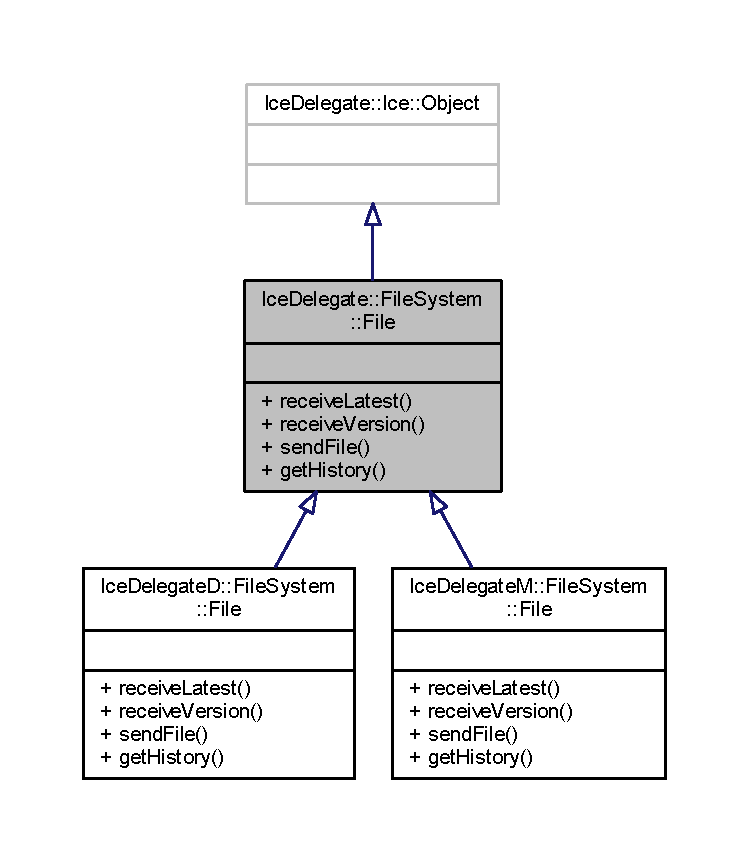
\includegraphics[width=350pt]{class_ice_delegate_1_1_file_system_1_1_file__inherit__graph}
\end{center}
\end{figure}


Collaboration diagram for Ice\+Delegate\+:\+:File\+System\+:\+:File\+:
\nopagebreak
\begin{figure}[H]
\begin{center}
\leavevmode
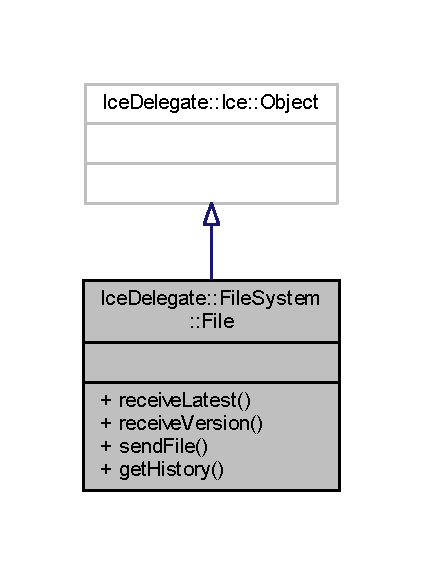
\includegraphics[width=203pt]{class_ice_delegate_1_1_file_system_1_1_file__coll__graph}
\end{center}
\end{figure}
\subsection*{Public Member Functions}
\begin{DoxyCompactItemize}
\item 
virtual \+::\hyperlink{namespace_file_system_a5c85de065f9c451ae1d1dea2dacb68c5}{File\+System\+::\+Byte\+Seq} \hyperlink{class_ice_delegate_1_1_file_system_1_1_file_aa6c349d0af2414f01f67471cc77761cf}{receive\+Latest} (const \+::std\+::string \&, const \+::std\+::string \&, const \+::std\+::string \&, const \+::std\+::string \&, const \+::Ice\+::\+Context $\ast$,\+::Ice\+Internal\+::\+Invocation\+Observer \&)=0
\item 
virtual \+::\hyperlink{namespace_file_system_a5c85de065f9c451ae1d1dea2dacb68c5}{File\+System\+::\+Byte\+Seq} \hyperlink{class_ice_delegate_1_1_file_system_1_1_file_a97482e33e323674fce8cca71eb8a8a50}{receive\+Version} (const \+::std\+::string \&, const \+::std\+::string \&, const \+::std\+::string \&, const \+::std\+::string \&,\+::Ice\+::\+Int, const \+::Ice\+::\+Context $\ast$,\+::Ice\+Internal\+::\+Invocation\+Observer \&)=0
\item 
virtual bool \hyperlink{class_ice_delegate_1_1_file_system_1_1_file_acb09c75ad462eb1a243a1b80dbce0863}{send\+File} (const \+::std\+::string \&, const \+::std\+::string \&, const \+::std\+::string \&, const \+::std\+::string \&, const \+::\hyperlink{namespace_file_system_a5c85de065f9c451ae1d1dea2dacb68c5}{File\+System\+::\+Byte\+Seq} \&, const \+::Ice\+::\+Context $\ast$,\+::Ice\+Internal\+::\+Invocation\+Observer \&)=0
\item 
virtual \+::\hyperlink{namespace_file_system_ac32dc1eb34c060160b52edc7c4e37d6e}{File\+System\+::\+Ver\+Seq} \hyperlink{class_ice_delegate_1_1_file_system_1_1_file_a5748eda06b14d3aca032850b08fa56e0}{get\+History} (const \+::std\+::string \&, const \+::std\+::string \&, const \+::std\+::string \&, const \+::std\+::string \&, const \+::Ice\+::\+Context $\ast$,\+::Ice\+Internal\+::\+Invocation\+Observer \&)=0
\end{DoxyCompactItemize}


\subsection{Member Function Documentation}
\hypertarget{class_ice_delegate_1_1_file_system_1_1_file_a5748eda06b14d3aca032850b08fa56e0}{}\index{Ice\+Delegate\+::\+File\+System\+::\+File@{Ice\+Delegate\+::\+File\+System\+::\+File}!get\+History@{get\+History}}
\index{get\+History@{get\+History}!Ice\+Delegate\+::\+File\+System\+::\+File@{Ice\+Delegate\+::\+File\+System\+::\+File}}
\subsubsection[{get\+History}]{\setlength{\rightskip}{0pt plus 5cm}virtual \+::{\bf File\+System\+::\+Ver\+Seq} Ice\+Delegate\+::\+File\+System\+::\+File\+::get\+History (
\begin{DoxyParamCaption}
\item[{const \+::std\+::string \&}]{, }
\item[{const \+::std\+::string \&}]{, }
\item[{const \+::std\+::string \&}]{, }
\item[{const \+::std\+::string \&}]{, }
\item[{const \+::Ice\+::\+Context $\ast$}]{, }
\item[{\+::Ice\+Internal\+::\+Invocation\+Observer \&}]{}
\end{DoxyParamCaption}
)\hspace{0.3cm}{\ttfamily [pure virtual]}}\label{class_ice_delegate_1_1_file_system_1_1_file_a5748eda06b14d3aca032850b08fa56e0}


Implemented in \hyperlink{class_ice_delegate_d_1_1_file_system_1_1_file_a4c0d32d5c6c2ce51f5315e1f0dd4cf47}{Ice\+Delegate\+D\+::\+File\+System\+::\+File}, and \hyperlink{class_ice_delegate_m_1_1_file_system_1_1_file_a00359ab8faf34bdc93ee409fb5f9242e}{Ice\+Delegate\+M\+::\+File\+System\+::\+File}.

\hypertarget{class_ice_delegate_1_1_file_system_1_1_file_aa6c349d0af2414f01f67471cc77761cf}{}\index{Ice\+Delegate\+::\+File\+System\+::\+File@{Ice\+Delegate\+::\+File\+System\+::\+File}!receive\+Latest@{receive\+Latest}}
\index{receive\+Latest@{receive\+Latest}!Ice\+Delegate\+::\+File\+System\+::\+File@{Ice\+Delegate\+::\+File\+System\+::\+File}}
\subsubsection[{receive\+Latest}]{\setlength{\rightskip}{0pt plus 5cm}virtual \+::{\bf File\+System\+::\+Byte\+Seq} Ice\+Delegate\+::\+File\+System\+::\+File\+::receive\+Latest (
\begin{DoxyParamCaption}
\item[{const \+::std\+::string \&}]{, }
\item[{const \+::std\+::string \&}]{, }
\item[{const \+::std\+::string \&}]{, }
\item[{const \+::std\+::string \&}]{, }
\item[{const \+::Ice\+::\+Context $\ast$}]{, }
\item[{\+::Ice\+Internal\+::\+Invocation\+Observer \&}]{}
\end{DoxyParamCaption}
)\hspace{0.3cm}{\ttfamily [pure virtual]}}\label{class_ice_delegate_1_1_file_system_1_1_file_aa6c349d0af2414f01f67471cc77761cf}


Implemented in \hyperlink{class_ice_delegate_d_1_1_file_system_1_1_file_add54fa82d12f5bbbc8fcc00e44aa0438}{Ice\+Delegate\+D\+::\+File\+System\+::\+File}, and \hyperlink{class_ice_delegate_m_1_1_file_system_1_1_file_a85aeef385bf8dd2fe91165096851f7a6}{Ice\+Delegate\+M\+::\+File\+System\+::\+File}.

\hypertarget{class_ice_delegate_1_1_file_system_1_1_file_a97482e33e323674fce8cca71eb8a8a50}{}\index{Ice\+Delegate\+::\+File\+System\+::\+File@{Ice\+Delegate\+::\+File\+System\+::\+File}!receive\+Version@{receive\+Version}}
\index{receive\+Version@{receive\+Version}!Ice\+Delegate\+::\+File\+System\+::\+File@{Ice\+Delegate\+::\+File\+System\+::\+File}}
\subsubsection[{receive\+Version}]{\setlength{\rightskip}{0pt plus 5cm}virtual \+::{\bf File\+System\+::\+Byte\+Seq} Ice\+Delegate\+::\+File\+System\+::\+File\+::receive\+Version (
\begin{DoxyParamCaption}
\item[{const \+::std\+::string \&}]{, }
\item[{const \+::std\+::string \&}]{, }
\item[{const \+::std\+::string \&}]{, }
\item[{const \+::std\+::string \&}]{, }
\item[{\+::Ice\+::\+Int}]{, }
\item[{const \+::Ice\+::\+Context $\ast$}]{, }
\item[{\+::Ice\+Internal\+::\+Invocation\+Observer \&}]{}
\end{DoxyParamCaption}
)\hspace{0.3cm}{\ttfamily [pure virtual]}}\label{class_ice_delegate_1_1_file_system_1_1_file_a97482e33e323674fce8cca71eb8a8a50}


Implemented in \hyperlink{class_ice_delegate_d_1_1_file_system_1_1_file_ac1937c3e49ac89a8794073205558edea}{Ice\+Delegate\+D\+::\+File\+System\+::\+File}, and \hyperlink{class_ice_delegate_m_1_1_file_system_1_1_file_a561cf717ab881b9775a8f92993f74eac}{Ice\+Delegate\+M\+::\+File\+System\+::\+File}.

\hypertarget{class_ice_delegate_1_1_file_system_1_1_file_acb09c75ad462eb1a243a1b80dbce0863}{}\index{Ice\+Delegate\+::\+File\+System\+::\+File@{Ice\+Delegate\+::\+File\+System\+::\+File}!send\+File@{send\+File}}
\index{send\+File@{send\+File}!Ice\+Delegate\+::\+File\+System\+::\+File@{Ice\+Delegate\+::\+File\+System\+::\+File}}
\subsubsection[{send\+File}]{\setlength{\rightskip}{0pt plus 5cm}virtual bool Ice\+Delegate\+::\+File\+System\+::\+File\+::send\+File (
\begin{DoxyParamCaption}
\item[{const \+::std\+::string \&}]{, }
\item[{const \+::std\+::string \&}]{, }
\item[{const \+::std\+::string \&}]{, }
\item[{const \+::std\+::string \&}]{, }
\item[{const \+::{\bf File\+System\+::\+Byte\+Seq} \&}]{, }
\item[{const \+::Ice\+::\+Context $\ast$}]{, }
\item[{\+::Ice\+Internal\+::\+Invocation\+Observer \&}]{}
\end{DoxyParamCaption}
)\hspace{0.3cm}{\ttfamily [pure virtual]}}\label{class_ice_delegate_1_1_file_system_1_1_file_acb09c75ad462eb1a243a1b80dbce0863}


Implemented in \hyperlink{class_ice_delegate_d_1_1_file_system_1_1_file_a219881647e8715fbf6e0f76d172b72b1}{Ice\+Delegate\+D\+::\+File\+System\+::\+File}, and \hyperlink{class_ice_delegate_m_1_1_file_system_1_1_file_a47acd886ed6caae05e4ae93153e42104}{Ice\+Delegate\+M\+::\+File\+System\+::\+File}.



The documentation for this class was generated from the following file\+:\begin{DoxyCompactItemize}
\item 
\hyperlink{_file_system_8h}{File\+System.\+h}\end{DoxyCompactItemize}

\hypertarget{class_ice_delegate_m_1_1_file_system_1_1_file}{}\section{Ice\+Delegate\+M\+:\+:File\+System\+:\+:File Class Reference}
\label{class_ice_delegate_m_1_1_file_system_1_1_file}\index{Ice\+Delegate\+M\+::\+File\+System\+::\+File@{Ice\+Delegate\+M\+::\+File\+System\+::\+File}}


{\ttfamily \#include $<$File\+System.\+h$>$}



Inheritance diagram for Ice\+Delegate\+M\+:\+:File\+System\+:\+:File\+:
\nopagebreak
\begin{figure}[H]
\begin{center}
\leavevmode
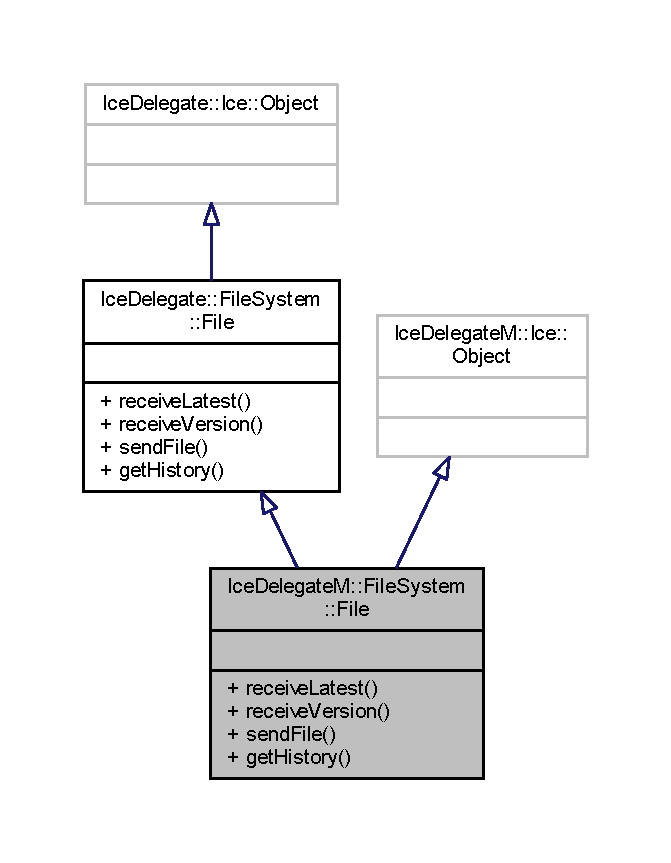
\includegraphics[width=322pt]{class_ice_delegate_m_1_1_file_system_1_1_file__inherit__graph}
\end{center}
\end{figure}


Collaboration diagram for Ice\+Delegate\+M\+:\+:File\+System\+:\+:File\+:
\nopagebreak
\begin{figure}[H]
\begin{center}
\leavevmode
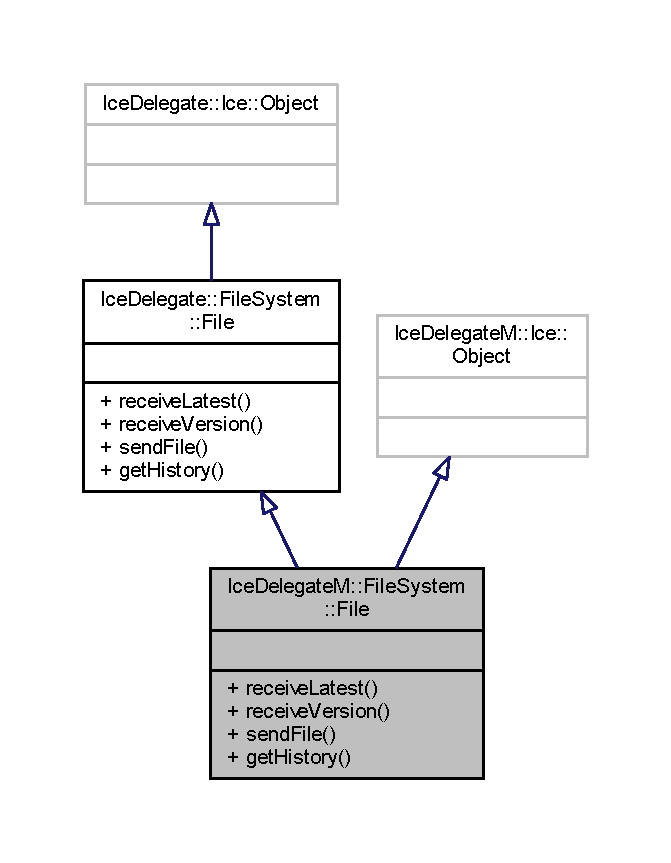
\includegraphics[width=322pt]{class_ice_delegate_m_1_1_file_system_1_1_file__coll__graph}
\end{center}
\end{figure}
\subsection*{Public Member Functions}
\begin{DoxyCompactItemize}
\item 
virtual \+::\hyperlink{namespace_file_system_a5c85de065f9c451ae1d1dea2dacb68c5}{File\+System\+::\+Byte\+Seq} \hyperlink{class_ice_delegate_m_1_1_file_system_1_1_file_a85aeef385bf8dd2fe91165096851f7a6}{receive\+Latest} (const \+::std\+::string \&, const \+::std\+::string \&, const \+::std\+::string \&, const \+::std\+::string \&, const \+::Ice\+::\+Context $\ast$,\+::Ice\+Internal\+::\+Invocation\+Observer \&)
\item 
virtual \+::\hyperlink{namespace_file_system_a5c85de065f9c451ae1d1dea2dacb68c5}{File\+System\+::\+Byte\+Seq} \hyperlink{class_ice_delegate_m_1_1_file_system_1_1_file_a561cf717ab881b9775a8f92993f74eac}{receive\+Version} (const \+::std\+::string \&, const \+::std\+::string \&, const \+::std\+::string \&, const \+::std\+::string \&,\+::Ice\+::\+Int, const \+::Ice\+::\+Context $\ast$,\+::Ice\+Internal\+::\+Invocation\+Observer \&)
\item 
virtual bool \hyperlink{class_ice_delegate_m_1_1_file_system_1_1_file_a47acd886ed6caae05e4ae93153e42104}{send\+File} (const \+::std\+::string \&, const \+::std\+::string \&, const \+::std\+::string \&, const \+::std\+::string \&, const \+::\hyperlink{namespace_file_system_a5c85de065f9c451ae1d1dea2dacb68c5}{File\+System\+::\+Byte\+Seq} \&, const \+::Ice\+::\+Context $\ast$,\+::Ice\+Internal\+::\+Invocation\+Observer \&)
\item 
virtual \+::\hyperlink{namespace_file_system_ac32dc1eb34c060160b52edc7c4e37d6e}{File\+System\+::\+Ver\+Seq} \hyperlink{class_ice_delegate_m_1_1_file_system_1_1_file_a00359ab8faf34bdc93ee409fb5f9242e}{get\+History} (const \+::std\+::string \&, const \+::std\+::string \&, const \+::std\+::string \&, const \+::std\+::string \&, const \+::Ice\+::\+Context $\ast$,\+::Ice\+Internal\+::\+Invocation\+Observer \&)
\end{DoxyCompactItemize}


\subsection{Member Function Documentation}
\hypertarget{class_ice_delegate_m_1_1_file_system_1_1_file_a00359ab8faf34bdc93ee409fb5f9242e}{}\index{Ice\+Delegate\+M\+::\+File\+System\+::\+File@{Ice\+Delegate\+M\+::\+File\+System\+::\+File}!get\+History@{get\+History}}
\index{get\+History@{get\+History}!Ice\+Delegate\+M\+::\+File\+System\+::\+File@{Ice\+Delegate\+M\+::\+File\+System\+::\+File}}
\subsubsection[{get\+History}]{\setlength{\rightskip}{0pt plus 5cm}{\bf File\+System\+::\+Ver\+Seq} Ice\+Delegate\+M\+::\+File\+System\+::\+File\+::get\+History (
\begin{DoxyParamCaption}
\item[{const \+::std\+::string \&}]{sec, }
\item[{const \+::std\+::string \&}]{art, }
\item[{const \+::std\+::string \&}]{type, }
\item[{const \+::std\+::string \&}]{f\+Name, }
\item[{const \+::Ice\+::\+Context $\ast$}]{\+\_\+\+\_\+context, }
\item[{\+::Ice\+Internal\+::\+Invocation\+Observer \&}]{\+\_\+\+\_\+observer}
\end{DoxyParamCaption}
)\hspace{0.3cm}{\ttfamily [virtual]}}\label{class_ice_delegate_m_1_1_file_system_1_1_file_a00359ab8faf34bdc93ee409fb5f9242e}


Implements \hyperlink{class_ice_delegate_1_1_file_system_1_1_file_a5748eda06b14d3aca032850b08fa56e0}{Ice\+Delegate\+::\+File\+System\+::\+File}.

\hypertarget{class_ice_delegate_m_1_1_file_system_1_1_file_a85aeef385bf8dd2fe91165096851f7a6}{}\index{Ice\+Delegate\+M\+::\+File\+System\+::\+File@{Ice\+Delegate\+M\+::\+File\+System\+::\+File}!receive\+Latest@{receive\+Latest}}
\index{receive\+Latest@{receive\+Latest}!Ice\+Delegate\+M\+::\+File\+System\+::\+File@{Ice\+Delegate\+M\+::\+File\+System\+::\+File}}
\subsubsection[{receive\+Latest}]{\setlength{\rightskip}{0pt plus 5cm}{\bf File\+System\+::\+Byte\+Seq} Ice\+Delegate\+M\+::\+File\+System\+::\+File\+::receive\+Latest (
\begin{DoxyParamCaption}
\item[{const \+::std\+::string \&}]{sec, }
\item[{const \+::std\+::string \&}]{art, }
\item[{const \+::std\+::string \&}]{type, }
\item[{const \+::std\+::string \&}]{f\+Name, }
\item[{const \+::Ice\+::\+Context $\ast$}]{\+\_\+\+\_\+context, }
\item[{\+::Ice\+Internal\+::\+Invocation\+Observer \&}]{\+\_\+\+\_\+observer}
\end{DoxyParamCaption}
)\hspace{0.3cm}{\ttfamily [virtual]}}\label{class_ice_delegate_m_1_1_file_system_1_1_file_a85aeef385bf8dd2fe91165096851f7a6}


Implements \hyperlink{class_ice_delegate_1_1_file_system_1_1_file_aa6c349d0af2414f01f67471cc77761cf}{Ice\+Delegate\+::\+File\+System\+::\+File}.

\hypertarget{class_ice_delegate_m_1_1_file_system_1_1_file_a561cf717ab881b9775a8f92993f74eac}{}\index{Ice\+Delegate\+M\+::\+File\+System\+::\+File@{Ice\+Delegate\+M\+::\+File\+System\+::\+File}!receive\+Version@{receive\+Version}}
\index{receive\+Version@{receive\+Version}!Ice\+Delegate\+M\+::\+File\+System\+::\+File@{Ice\+Delegate\+M\+::\+File\+System\+::\+File}}
\subsubsection[{receive\+Version}]{\setlength{\rightskip}{0pt plus 5cm}{\bf File\+System\+::\+Byte\+Seq} Ice\+Delegate\+M\+::\+File\+System\+::\+File\+::receive\+Version (
\begin{DoxyParamCaption}
\item[{const \+::std\+::string \&}]{sec, }
\item[{const \+::std\+::string \&}]{art, }
\item[{const \+::std\+::string \&}]{type, }
\item[{const \+::std\+::string \&}]{f\+Name, }
\item[{\+::Ice\+::\+Int}]{ver, }
\item[{const \+::Ice\+::\+Context $\ast$}]{\+\_\+\+\_\+context, }
\item[{\+::Ice\+Internal\+::\+Invocation\+Observer \&}]{\+\_\+\+\_\+observer}
\end{DoxyParamCaption}
)\hspace{0.3cm}{\ttfamily [virtual]}}\label{class_ice_delegate_m_1_1_file_system_1_1_file_a561cf717ab881b9775a8f92993f74eac}


Implements \hyperlink{class_ice_delegate_1_1_file_system_1_1_file_a97482e33e323674fce8cca71eb8a8a50}{Ice\+Delegate\+::\+File\+System\+::\+File}.

\hypertarget{class_ice_delegate_m_1_1_file_system_1_1_file_a47acd886ed6caae05e4ae93153e42104}{}\index{Ice\+Delegate\+M\+::\+File\+System\+::\+File@{Ice\+Delegate\+M\+::\+File\+System\+::\+File}!send\+File@{send\+File}}
\index{send\+File@{send\+File}!Ice\+Delegate\+M\+::\+File\+System\+::\+File@{Ice\+Delegate\+M\+::\+File\+System\+::\+File}}
\subsubsection[{send\+File}]{\setlength{\rightskip}{0pt plus 5cm}bool Ice\+Delegate\+M\+::\+File\+System\+::\+File\+::send\+File (
\begin{DoxyParamCaption}
\item[{const \+::std\+::string \&}]{sec, }
\item[{const \+::std\+::string \&}]{art, }
\item[{const \+::std\+::string \&}]{type, }
\item[{const \+::std\+::string \&}]{f\+Name\+Ext, }
\item[{const \+::{\bf File\+System\+::\+Byte\+Seq} \&}]{seq, }
\item[{const \+::Ice\+::\+Context $\ast$}]{\+\_\+\+\_\+context, }
\item[{\+::Ice\+Internal\+::\+Invocation\+Observer \&}]{\+\_\+\+\_\+observer}
\end{DoxyParamCaption}
)\hspace{0.3cm}{\ttfamily [virtual]}}\label{class_ice_delegate_m_1_1_file_system_1_1_file_a47acd886ed6caae05e4ae93153e42104}


Implements \hyperlink{class_ice_delegate_1_1_file_system_1_1_file_acb09c75ad462eb1a243a1b80dbce0863}{Ice\+Delegate\+::\+File\+System\+::\+File}.



The documentation for this class was generated from the following files\+:\begin{DoxyCompactItemize}
\item 
\hyperlink{_file_system_8h}{File\+System.\+h}\item 
\hyperlink{_file_system_8cpp}{File\+System.\+cpp}\end{DoxyCompactItemize}

\hypertarget{class_ice_delegate_d_1_1_file_system_1_1_file}{}\section{Ice\+Delegate\+D\+:\+:File\+System\+:\+:File Class Reference}
\label{class_ice_delegate_d_1_1_file_system_1_1_file}\index{Ice\+Delegate\+D\+::\+File\+System\+::\+File@{Ice\+Delegate\+D\+::\+File\+System\+::\+File}}


{\ttfamily \#include $<$File\+System.\+h$>$}



Inheritance diagram for Ice\+Delegate\+D\+:\+:File\+System\+:\+:File\+:
\nopagebreak
\begin{figure}[H]
\begin{center}
\leavevmode
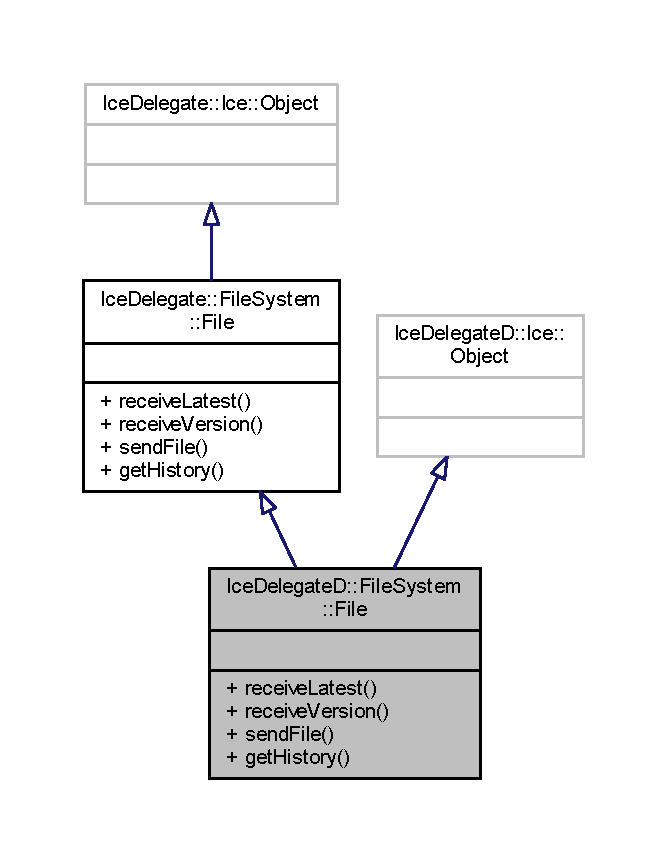
\includegraphics[width=320pt]{class_ice_delegate_d_1_1_file_system_1_1_file__inherit__graph}
\end{center}
\end{figure}


Collaboration diagram for Ice\+Delegate\+D\+:\+:File\+System\+:\+:File\+:
\nopagebreak
\begin{figure}[H]
\begin{center}
\leavevmode
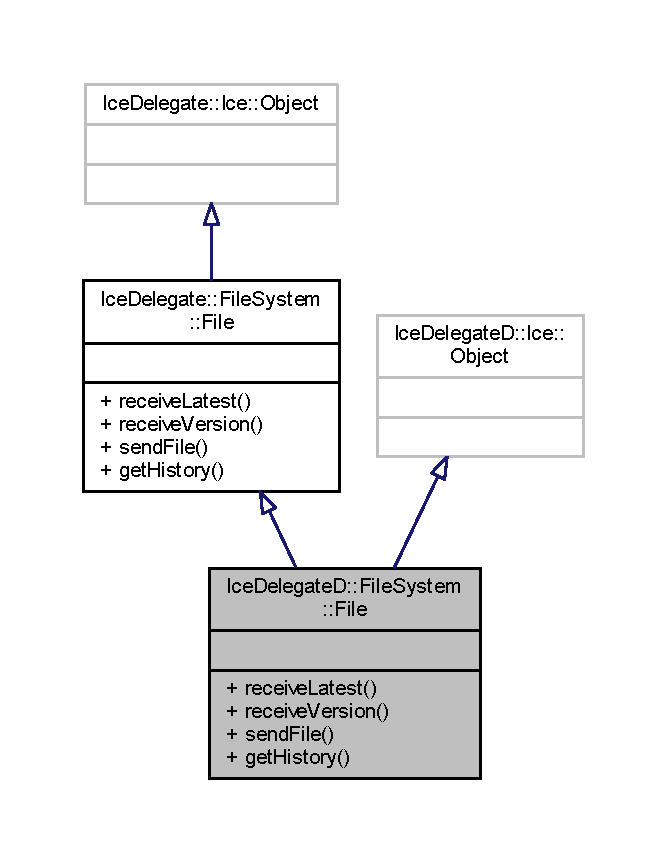
\includegraphics[width=320pt]{class_ice_delegate_d_1_1_file_system_1_1_file__coll__graph}
\end{center}
\end{figure}
\subsection*{Public Member Functions}
\begin{DoxyCompactItemize}
\item 
virtual \+::\hyperlink{namespace_file_system_a5c85de065f9c451ae1d1dea2dacb68c5}{File\+System\+::\+Byte\+Seq} \hyperlink{class_ice_delegate_d_1_1_file_system_1_1_file_add54fa82d12f5bbbc8fcc00e44aa0438}{receive\+Latest} (const \+::std\+::string \&, const \+::std\+::string \&, const \+::std\+::string \&, const \+::std\+::string \&, const \+::Ice\+::\+Context $\ast$,\+::Ice\+Internal\+::\+Invocation\+Observer \&)
\item 
virtual \+::\hyperlink{namespace_file_system_a5c85de065f9c451ae1d1dea2dacb68c5}{File\+System\+::\+Byte\+Seq} \hyperlink{class_ice_delegate_d_1_1_file_system_1_1_file_ac1937c3e49ac89a8794073205558edea}{receive\+Version} (const \+::std\+::string \&, const \+::std\+::string \&, const \+::std\+::string \&, const \+::std\+::string \&,\+::Ice\+::\+Int, const \+::Ice\+::\+Context $\ast$,\+::Ice\+Internal\+::\+Invocation\+Observer \&)
\item 
virtual bool \hyperlink{class_ice_delegate_d_1_1_file_system_1_1_file_a219881647e8715fbf6e0f76d172b72b1}{send\+File} (const \+::std\+::string \&, const \+::std\+::string \&, const \+::std\+::string \&, const \+::std\+::string \&, const \+::\hyperlink{namespace_file_system_a5c85de065f9c451ae1d1dea2dacb68c5}{File\+System\+::\+Byte\+Seq} \&, const \+::Ice\+::\+Context $\ast$,\+::Ice\+Internal\+::\+Invocation\+Observer \&)
\item 
virtual \+::\hyperlink{namespace_file_system_ac32dc1eb34c060160b52edc7c4e37d6e}{File\+System\+::\+Ver\+Seq} \hyperlink{class_ice_delegate_d_1_1_file_system_1_1_file_a4c0d32d5c6c2ce51f5315e1f0dd4cf47}{get\+History} (const \+::std\+::string \&, const \+::std\+::string \&, const \+::std\+::string \&, const \+::std\+::string \&, const \+::Ice\+::\+Context $\ast$,\+::Ice\+Internal\+::\+Invocation\+Observer \&)
\end{DoxyCompactItemize}


\subsection{Member Function Documentation}
\hypertarget{class_ice_delegate_d_1_1_file_system_1_1_file_a4c0d32d5c6c2ce51f5315e1f0dd4cf47}{}\index{Ice\+Delegate\+D\+::\+File\+System\+::\+File@{Ice\+Delegate\+D\+::\+File\+System\+::\+File}!get\+History@{get\+History}}
\index{get\+History@{get\+History}!Ice\+Delegate\+D\+::\+File\+System\+::\+File@{Ice\+Delegate\+D\+::\+File\+System\+::\+File}}
\subsubsection[{get\+History}]{\setlength{\rightskip}{0pt plus 5cm}{\bf File\+System\+::\+Ver\+Seq} Ice\+Delegate\+D\+::\+File\+System\+::\+File\+::get\+History (
\begin{DoxyParamCaption}
\item[{const \+::std\+::string \&}]{sec, }
\item[{const \+::std\+::string \&}]{art, }
\item[{const \+::std\+::string \&}]{type, }
\item[{const \+::std\+::string \&}]{f\+Name, }
\item[{const \+::Ice\+::\+Context $\ast$}]{\+\_\+\+\_\+context, }
\item[{\+::Ice\+Internal\+::\+Invocation\+Observer \&}]{}
\end{DoxyParamCaption}
)\hspace{0.3cm}{\ttfamily [virtual]}}\label{class_ice_delegate_d_1_1_file_system_1_1_file_a4c0d32d5c6c2ce51f5315e1f0dd4cf47}


Implements \hyperlink{class_ice_delegate_1_1_file_system_1_1_file_a5748eda06b14d3aca032850b08fa56e0}{Ice\+Delegate\+::\+File\+System\+::\+File}.



Here is the call graph for this function\+:
\nopagebreak
\begin{figure}[H]
\begin{center}
\leavevmode
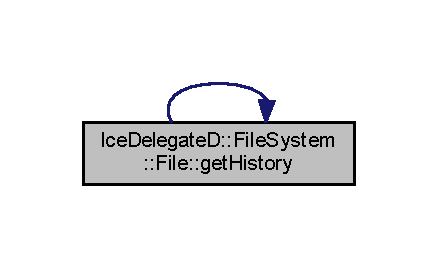
\includegraphics[width=210pt]{class_ice_delegate_d_1_1_file_system_1_1_file_a4c0d32d5c6c2ce51f5315e1f0dd4cf47_cgraph}
\end{center}
\end{figure}




Here is the caller graph for this function\+:
\nopagebreak
\begin{figure}[H]
\begin{center}
\leavevmode
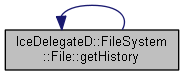
\includegraphics[width=210pt]{class_ice_delegate_d_1_1_file_system_1_1_file_a4c0d32d5c6c2ce51f5315e1f0dd4cf47_icgraph}
\end{center}
\end{figure}


\hypertarget{class_ice_delegate_d_1_1_file_system_1_1_file_add54fa82d12f5bbbc8fcc00e44aa0438}{}\index{Ice\+Delegate\+D\+::\+File\+System\+::\+File@{Ice\+Delegate\+D\+::\+File\+System\+::\+File}!receive\+Latest@{receive\+Latest}}
\index{receive\+Latest@{receive\+Latest}!Ice\+Delegate\+D\+::\+File\+System\+::\+File@{Ice\+Delegate\+D\+::\+File\+System\+::\+File}}
\subsubsection[{receive\+Latest}]{\setlength{\rightskip}{0pt plus 5cm}{\bf File\+System\+::\+Byte\+Seq} Ice\+Delegate\+D\+::\+File\+System\+::\+File\+::receive\+Latest (
\begin{DoxyParamCaption}
\item[{const \+::std\+::string \&}]{sec, }
\item[{const \+::std\+::string \&}]{art, }
\item[{const \+::std\+::string \&}]{type, }
\item[{const \+::std\+::string \&}]{f\+Name, }
\item[{const \+::Ice\+::\+Context $\ast$}]{\+\_\+\+\_\+context, }
\item[{\+::Ice\+Internal\+::\+Invocation\+Observer \&}]{}
\end{DoxyParamCaption}
)\hspace{0.3cm}{\ttfamily [virtual]}}\label{class_ice_delegate_d_1_1_file_system_1_1_file_add54fa82d12f5bbbc8fcc00e44aa0438}


Implements \hyperlink{class_ice_delegate_1_1_file_system_1_1_file_aa6c349d0af2414f01f67471cc77761cf}{Ice\+Delegate\+::\+File\+System\+::\+File}.



Here is the call graph for this function\+:
\nopagebreak
\begin{figure}[H]
\begin{center}
\leavevmode
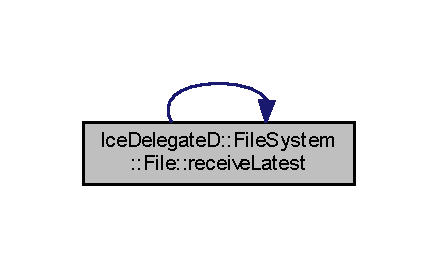
\includegraphics[width=210pt]{class_ice_delegate_d_1_1_file_system_1_1_file_add54fa82d12f5bbbc8fcc00e44aa0438_cgraph}
\end{center}
\end{figure}




Here is the caller graph for this function\+:
\nopagebreak
\begin{figure}[H]
\begin{center}
\leavevmode
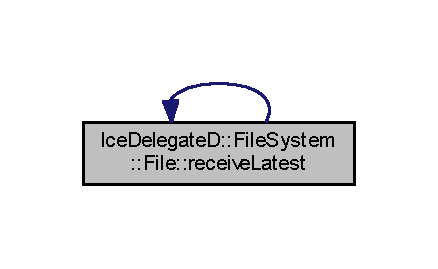
\includegraphics[width=210pt]{class_ice_delegate_d_1_1_file_system_1_1_file_add54fa82d12f5bbbc8fcc00e44aa0438_icgraph}
\end{center}
\end{figure}


\hypertarget{class_ice_delegate_d_1_1_file_system_1_1_file_ac1937c3e49ac89a8794073205558edea}{}\index{Ice\+Delegate\+D\+::\+File\+System\+::\+File@{Ice\+Delegate\+D\+::\+File\+System\+::\+File}!receive\+Version@{receive\+Version}}
\index{receive\+Version@{receive\+Version}!Ice\+Delegate\+D\+::\+File\+System\+::\+File@{Ice\+Delegate\+D\+::\+File\+System\+::\+File}}
\subsubsection[{receive\+Version}]{\setlength{\rightskip}{0pt plus 5cm}{\bf File\+System\+::\+Byte\+Seq} Ice\+Delegate\+D\+::\+File\+System\+::\+File\+::receive\+Version (
\begin{DoxyParamCaption}
\item[{const \+::std\+::string \&}]{sec, }
\item[{const \+::std\+::string \&}]{art, }
\item[{const \+::std\+::string \&}]{type, }
\item[{const \+::std\+::string \&}]{f\+Name, }
\item[{\+::Ice\+::\+Int}]{ver, }
\item[{const \+::Ice\+::\+Context $\ast$}]{\+\_\+\+\_\+context, }
\item[{\+::Ice\+Internal\+::\+Invocation\+Observer \&}]{}
\end{DoxyParamCaption}
)\hspace{0.3cm}{\ttfamily [virtual]}}\label{class_ice_delegate_d_1_1_file_system_1_1_file_ac1937c3e49ac89a8794073205558edea}


Implements \hyperlink{class_ice_delegate_1_1_file_system_1_1_file_a97482e33e323674fce8cca71eb8a8a50}{Ice\+Delegate\+::\+File\+System\+::\+File}.



Here is the call graph for this function\+:
\nopagebreak
\begin{figure}[H]
\begin{center}
\leavevmode
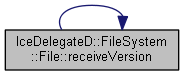
\includegraphics[width=210pt]{class_ice_delegate_d_1_1_file_system_1_1_file_ac1937c3e49ac89a8794073205558edea_cgraph}
\end{center}
\end{figure}




Here is the caller graph for this function\+:
\nopagebreak
\begin{figure}[H]
\begin{center}
\leavevmode
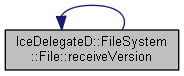
\includegraphics[width=210pt]{class_ice_delegate_d_1_1_file_system_1_1_file_ac1937c3e49ac89a8794073205558edea_icgraph}
\end{center}
\end{figure}


\hypertarget{class_ice_delegate_d_1_1_file_system_1_1_file_a219881647e8715fbf6e0f76d172b72b1}{}\index{Ice\+Delegate\+D\+::\+File\+System\+::\+File@{Ice\+Delegate\+D\+::\+File\+System\+::\+File}!send\+File@{send\+File}}
\index{send\+File@{send\+File}!Ice\+Delegate\+D\+::\+File\+System\+::\+File@{Ice\+Delegate\+D\+::\+File\+System\+::\+File}}
\subsubsection[{send\+File}]{\setlength{\rightskip}{0pt plus 5cm}bool Ice\+Delegate\+D\+::\+File\+System\+::\+File\+::send\+File (
\begin{DoxyParamCaption}
\item[{const \+::std\+::string \&}]{sec, }
\item[{const \+::std\+::string \&}]{art, }
\item[{const \+::std\+::string \&}]{type, }
\item[{const \+::std\+::string \&}]{f\+Name\+Ext, }
\item[{const \+::{\bf File\+System\+::\+Byte\+Seq} \&}]{seq, }
\item[{const \+::Ice\+::\+Context $\ast$}]{\+\_\+\+\_\+context, }
\item[{\+::Ice\+Internal\+::\+Invocation\+Observer \&}]{}
\end{DoxyParamCaption}
)\hspace{0.3cm}{\ttfamily [virtual]}}\label{class_ice_delegate_d_1_1_file_system_1_1_file_a219881647e8715fbf6e0f76d172b72b1}


Implements \hyperlink{class_ice_delegate_1_1_file_system_1_1_file_acb09c75ad462eb1a243a1b80dbce0863}{Ice\+Delegate\+::\+File\+System\+::\+File}.



Here is the call graph for this function\+:
\nopagebreak
\begin{figure}[H]
\begin{center}
\leavevmode
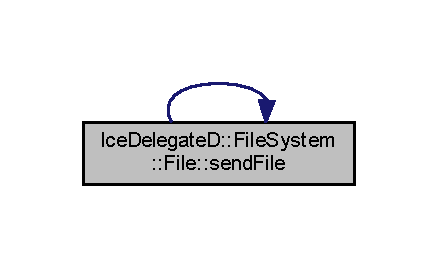
\includegraphics[width=210pt]{class_ice_delegate_d_1_1_file_system_1_1_file_a219881647e8715fbf6e0f76d172b72b1_cgraph}
\end{center}
\end{figure}




Here is the caller graph for this function\+:
\nopagebreak
\begin{figure}[H]
\begin{center}
\leavevmode
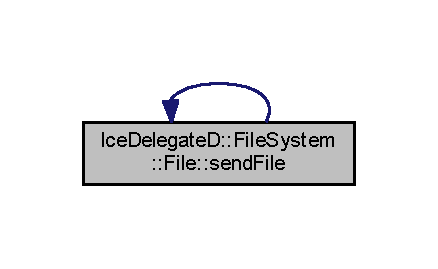
\includegraphics[width=210pt]{class_ice_delegate_d_1_1_file_system_1_1_file_a219881647e8715fbf6e0f76d172b72b1_icgraph}
\end{center}
\end{figure}




The documentation for this class was generated from the following files\+:\begin{DoxyCompactItemize}
\item 
\hyperlink{_file_system_8h}{File\+System.\+h}\item 
\hyperlink{_file_system_8cpp}{File\+System.\+cpp}\end{DoxyCompactItemize}

\hypertarget{class_file_system_1_1_file}{}\section{File\+System\+:\+:File Class Reference}
\label{class_file_system_1_1_file}\index{File\+System\+::\+File@{File\+System\+::\+File}}


{\ttfamily \#include $<$File\+System.\+h$>$}



Inheritance diagram for File\+System\+:\+:File\+:
\nopagebreak
\begin{figure}[H]
\begin{center}
\leavevmode
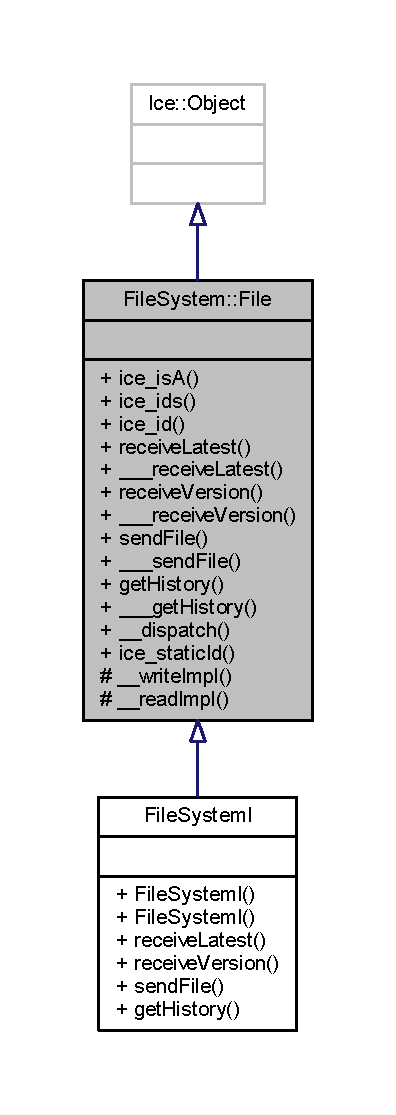
\includegraphics[width=190pt]{class_file_system_1_1_file__inherit__graph}
\end{center}
\end{figure}


Collaboration diagram for File\+System\+:\+:File\+:
\nopagebreak
\begin{figure}[H]
\begin{center}
\leavevmode
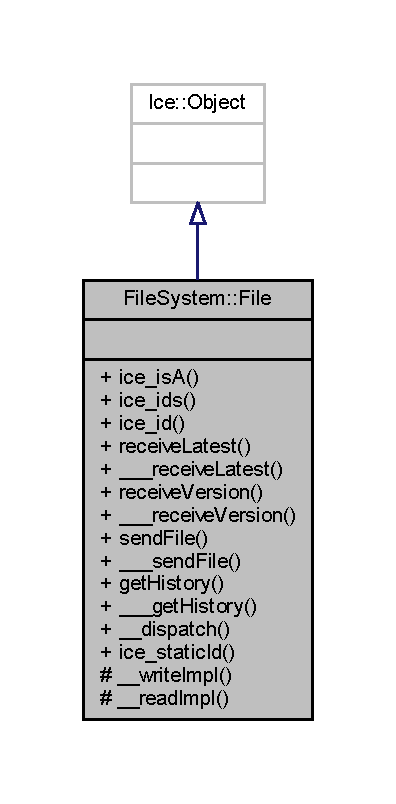
\includegraphics[width=190pt]{class_file_system_1_1_file__coll__graph}
\end{center}
\end{figure}
\subsection*{Public Types}
\begin{DoxyCompactItemize}
\item 
typedef \hyperlink{namespace_file_system_a2cca5b42d5ab231d91dd889d4d74218c}{File\+Prx} \hyperlink{class_file_system_1_1_file_a2dc305348e01c17ad9736a7abcbec36e}{Proxy\+Type}
\item 
typedef \hyperlink{namespace_file_system_a322304ec4ae6dc6308f79d49662764bb}{File\+Ptr} \hyperlink{class_file_system_1_1_file_a51b2a288a025efc05fb07e0dfb29f06f}{Pointer\+Type}
\end{DoxyCompactItemize}
\subsection*{Public Member Functions}
\begin{DoxyCompactItemize}
\item 
virtual bool \hyperlink{class_file_system_1_1_file_afec97134dcddcbbc8f71facb63fab3a1}{ice\+\_\+is\+A} (const \+::std\+::string \&, const \+::Ice\+::\+Current \&=\+::Ice\+::\+Current()) const 
\item 
virtual \+::std\+::vector$<$ \+::std\+::string $>$ \hyperlink{class_file_system_1_1_file_abab4030df236aaeaba1f11025ad8a44e}{ice\+\_\+ids} (const \+::Ice\+::\+Current \&=\+::Ice\+::\+Current()) const 
\item 
virtual const \+::std\+::string \& \hyperlink{class_file_system_1_1_file_ab914ee68ffbae6780d679fad367157aa}{ice\+\_\+id} (const \+::Ice\+::\+Current \&=\+::Ice\+::\+Current()) const 
\item 
virtual \+::\hyperlink{namespace_file_system_a5c85de065f9c451ae1d1dea2dacb68c5}{File\+System\+::\+Byte\+Seq} \hyperlink{class_file_system_1_1_file_a99b432d430b47e2f065cf9ad529c8956}{receive\+Latest} (const \+::std\+::string \&, const \+::std\+::string \&, const \+::std\+::string \&, const \+::std\+::string \&, const \+::Ice\+::\+Current \&=\+::Ice\+::\+Current())=0
\item 
\+::Ice\+::\+Dispatch\+Status \hyperlink{class_file_system_1_1_file_a26bd114faec6b1c85d119ff4a0e57ca1}{\+\_\+\+\_\+\+\_\+receive\+Latest} (\+::Ice\+Internal\+::\+Incoming \&, const \+::Ice\+::\+Current \&)
\item 
virtual \+::\hyperlink{namespace_file_system_a5c85de065f9c451ae1d1dea2dacb68c5}{File\+System\+::\+Byte\+Seq} \hyperlink{class_file_system_1_1_file_a135c7e7f7f7838e6c76c36cdf0012131}{receive\+Version} (const \+::std\+::string \&, const \+::std\+::string \&, const \+::std\+::string \&, const \+::std\+::string \&,\+::Ice\+::\+Int, const \+::Ice\+::\+Current \&=\+::Ice\+::\+Current())=0
\item 
\+::Ice\+::\+Dispatch\+Status \hyperlink{class_file_system_1_1_file_a96c6caf4d0270443e84f1fb4548e3de8}{\+\_\+\+\_\+\+\_\+receive\+Version} (\+::Ice\+Internal\+::\+Incoming \&, const \+::Ice\+::\+Current \&)
\item 
virtual bool \hyperlink{class_file_system_1_1_file_a06849361bc722ed92f0075377eac6d09}{send\+File} (const \+::std\+::string \&, const \+::std\+::string \&, const \+::std\+::string \&, const \+::std\+::string \&, const \+::\hyperlink{namespace_file_system_a5c85de065f9c451ae1d1dea2dacb68c5}{File\+System\+::\+Byte\+Seq} \&, const \+::Ice\+::\+Current \&=\+::Ice\+::\+Current())=0
\item 
\+::Ice\+::\+Dispatch\+Status \hyperlink{class_file_system_1_1_file_a0259134b0777f587ee8b38dd08831a0c}{\+\_\+\+\_\+\+\_\+send\+File} (\+::Ice\+Internal\+::\+Incoming \&, const \+::Ice\+::\+Current \&)
\item 
virtual \+::\hyperlink{namespace_file_system_ac32dc1eb34c060160b52edc7c4e37d6e}{File\+System\+::\+Ver\+Seq} \hyperlink{class_file_system_1_1_file_aa411c511900735474fdba5f9c22a1747}{get\+History} (const \+::std\+::string \&, const \+::std\+::string \&, const \+::std\+::string \&, const \+::std\+::string \&, const \+::Ice\+::\+Current \&=\+::Ice\+::\+Current())=0
\item 
\+::Ice\+::\+Dispatch\+Status \hyperlink{class_file_system_1_1_file_a5798e84a210ecbe73bc52062d9c44019}{\+\_\+\+\_\+\+\_\+get\+History} (\+::Ice\+Internal\+::\+Incoming \&, const \+::Ice\+::\+Current \&)
\item 
virtual \+::Ice\+::\+Dispatch\+Status \hyperlink{class_file_system_1_1_file_a245efe96625966b4d5dc6c70b6f5eae8}{\+\_\+\+\_\+dispatch} (\+::Ice\+Internal\+::\+Incoming \&, const \+::Ice\+::\+Current \&)
\end{DoxyCompactItemize}
\subsection*{Static Public Member Functions}
\begin{DoxyCompactItemize}
\item 
static const \+::std\+::string \& \hyperlink{class_file_system_1_1_file_ad7894f231547d245a095e12fc557dc2c}{ice\+\_\+static\+Id} ()
\end{DoxyCompactItemize}
\subsection*{Protected Member Functions}
\begin{DoxyCompactItemize}
\item 
virtual void \hyperlink{class_file_system_1_1_file_a2ba83e5fbc37577fb08f6cc44b1006e2}{\+\_\+\+\_\+write\+Impl} (\+::Ice\+Internal\+::\+Basic\+Stream $\ast$) const 
\item 
virtual void \hyperlink{class_file_system_1_1_file_af70b25b7133fa3f2be82b8b8ce37b852}{\+\_\+\+\_\+read\+Impl} (\+::Ice\+Internal\+::\+Basic\+Stream $\ast$)
\end{DoxyCompactItemize}


\subsection{Member Typedef Documentation}
\hypertarget{class_file_system_1_1_file_a51b2a288a025efc05fb07e0dfb29f06f}{}\index{File\+System\+::\+File@{File\+System\+::\+File}!Pointer\+Type@{Pointer\+Type}}
\index{Pointer\+Type@{Pointer\+Type}!File\+System\+::\+File@{File\+System\+::\+File}}
\subsubsection[{Pointer\+Type}]{\setlength{\rightskip}{0pt plus 5cm}typedef {\bf File\+Ptr} {\bf File\+System\+::\+File\+::\+Pointer\+Type}}\label{class_file_system_1_1_file_a51b2a288a025efc05fb07e0dfb29f06f}
\hypertarget{class_file_system_1_1_file_a2dc305348e01c17ad9736a7abcbec36e}{}\index{File\+System\+::\+File@{File\+System\+::\+File}!Proxy\+Type@{Proxy\+Type}}
\index{Proxy\+Type@{Proxy\+Type}!File\+System\+::\+File@{File\+System\+::\+File}}
\subsubsection[{Proxy\+Type}]{\setlength{\rightskip}{0pt plus 5cm}typedef {\bf File\+Prx} {\bf File\+System\+::\+File\+::\+Proxy\+Type}}\label{class_file_system_1_1_file_a2dc305348e01c17ad9736a7abcbec36e}


\subsection{Member Function Documentation}
\hypertarget{class_file_system_1_1_file_a5798e84a210ecbe73bc52062d9c44019}{}\index{File\+System\+::\+File@{File\+System\+::\+File}!\+\_\+\+\_\+\+\_\+get\+History@{\+\_\+\+\_\+\+\_\+get\+History}}
\index{\+\_\+\+\_\+\+\_\+get\+History@{\+\_\+\+\_\+\+\_\+get\+History}!File\+System\+::\+File@{File\+System\+::\+File}}
\subsubsection[{\+\_\+\+\_\+\+\_\+get\+History}]{\setlength{\rightskip}{0pt plus 5cm}Ice\+::\+Dispatch\+Status File\+System\+::\+File\+::\+\_\+\+\_\+\+\_\+get\+History (
\begin{DoxyParamCaption}
\item[{\+::Ice\+Internal\+::\+Incoming \&}]{\+\_\+\+\_\+in\+S, }
\item[{const \+::Ice\+::\+Current \&}]{\+\_\+\+\_\+current}
\end{DoxyParamCaption}
)}\label{class_file_system_1_1_file_a5798e84a210ecbe73bc52062d9c44019}
\hypertarget{class_file_system_1_1_file_a26bd114faec6b1c85d119ff4a0e57ca1}{}\index{File\+System\+::\+File@{File\+System\+::\+File}!\+\_\+\+\_\+\+\_\+receive\+Latest@{\+\_\+\+\_\+\+\_\+receive\+Latest}}
\index{\+\_\+\+\_\+\+\_\+receive\+Latest@{\+\_\+\+\_\+\+\_\+receive\+Latest}!File\+System\+::\+File@{File\+System\+::\+File}}
\subsubsection[{\+\_\+\+\_\+\+\_\+receive\+Latest}]{\setlength{\rightskip}{0pt plus 5cm}Ice\+::\+Dispatch\+Status File\+System\+::\+File\+::\+\_\+\+\_\+\+\_\+receive\+Latest (
\begin{DoxyParamCaption}
\item[{\+::Ice\+Internal\+::\+Incoming \&}]{\+\_\+\+\_\+in\+S, }
\item[{const \+::Ice\+::\+Current \&}]{\+\_\+\+\_\+current}
\end{DoxyParamCaption}
)}\label{class_file_system_1_1_file_a26bd114faec6b1c85d119ff4a0e57ca1}
\hypertarget{class_file_system_1_1_file_a96c6caf4d0270443e84f1fb4548e3de8}{}\index{File\+System\+::\+File@{File\+System\+::\+File}!\+\_\+\+\_\+\+\_\+receive\+Version@{\+\_\+\+\_\+\+\_\+receive\+Version}}
\index{\+\_\+\+\_\+\+\_\+receive\+Version@{\+\_\+\+\_\+\+\_\+receive\+Version}!File\+System\+::\+File@{File\+System\+::\+File}}
\subsubsection[{\+\_\+\+\_\+\+\_\+receive\+Version}]{\setlength{\rightskip}{0pt plus 5cm}Ice\+::\+Dispatch\+Status File\+System\+::\+File\+::\+\_\+\+\_\+\+\_\+receive\+Version (
\begin{DoxyParamCaption}
\item[{\+::Ice\+Internal\+::\+Incoming \&}]{\+\_\+\+\_\+in\+S, }
\item[{const \+::Ice\+::\+Current \&}]{\+\_\+\+\_\+current}
\end{DoxyParamCaption}
)}\label{class_file_system_1_1_file_a96c6caf4d0270443e84f1fb4548e3de8}
\hypertarget{class_file_system_1_1_file_a0259134b0777f587ee8b38dd08831a0c}{}\index{File\+System\+::\+File@{File\+System\+::\+File}!\+\_\+\+\_\+\+\_\+send\+File@{\+\_\+\+\_\+\+\_\+send\+File}}
\index{\+\_\+\+\_\+\+\_\+send\+File@{\+\_\+\+\_\+\+\_\+send\+File}!File\+System\+::\+File@{File\+System\+::\+File}}
\subsubsection[{\+\_\+\+\_\+\+\_\+send\+File}]{\setlength{\rightskip}{0pt plus 5cm}Ice\+::\+Dispatch\+Status File\+System\+::\+File\+::\+\_\+\+\_\+\+\_\+send\+File (
\begin{DoxyParamCaption}
\item[{\+::Ice\+Internal\+::\+Incoming \&}]{\+\_\+\+\_\+in\+S, }
\item[{const \+::Ice\+::\+Current \&}]{\+\_\+\+\_\+current}
\end{DoxyParamCaption}
)}\label{class_file_system_1_1_file_a0259134b0777f587ee8b38dd08831a0c}
\hypertarget{class_file_system_1_1_file_a245efe96625966b4d5dc6c70b6f5eae8}{}\index{File\+System\+::\+File@{File\+System\+::\+File}!\+\_\+\+\_\+dispatch@{\+\_\+\+\_\+dispatch}}
\index{\+\_\+\+\_\+dispatch@{\+\_\+\+\_\+dispatch}!File\+System\+::\+File@{File\+System\+::\+File}}
\subsubsection[{\+\_\+\+\_\+dispatch}]{\setlength{\rightskip}{0pt plus 5cm}Ice\+::\+Dispatch\+Status File\+System\+::\+File\+::\+\_\+\+\_\+dispatch (
\begin{DoxyParamCaption}
\item[{\+::Ice\+Internal\+::\+Incoming \&}]{in, }
\item[{const \+::Ice\+::\+Current \&}]{current}
\end{DoxyParamCaption}
)}\label{class_file_system_1_1_file_a245efe96625966b4d5dc6c70b6f5eae8}
\hypertarget{class_file_system_1_1_file_af70b25b7133fa3f2be82b8b8ce37b852}{}\index{File\+System\+::\+File@{File\+System\+::\+File}!\+\_\+\+\_\+read\+Impl@{\+\_\+\+\_\+read\+Impl}}
\index{\+\_\+\+\_\+read\+Impl@{\+\_\+\+\_\+read\+Impl}!File\+System\+::\+File@{File\+System\+::\+File}}
\subsubsection[{\+\_\+\+\_\+read\+Impl}]{\setlength{\rightskip}{0pt plus 5cm}void File\+System\+::\+File\+::\+\_\+\+\_\+read\+Impl (
\begin{DoxyParamCaption}
\item[{\+::Ice\+Internal\+::\+Basic\+Stream $\ast$}]{\+\_\+\+\_\+is}
\end{DoxyParamCaption}
)\hspace{0.3cm}{\ttfamily [protected]}, {\ttfamily [virtual]}}\label{class_file_system_1_1_file_af70b25b7133fa3f2be82b8b8ce37b852}
\hypertarget{class_file_system_1_1_file_a2ba83e5fbc37577fb08f6cc44b1006e2}{}\index{File\+System\+::\+File@{File\+System\+::\+File}!\+\_\+\+\_\+write\+Impl@{\+\_\+\+\_\+write\+Impl}}
\index{\+\_\+\+\_\+write\+Impl@{\+\_\+\+\_\+write\+Impl}!File\+System\+::\+File@{File\+System\+::\+File}}
\subsubsection[{\+\_\+\+\_\+write\+Impl}]{\setlength{\rightskip}{0pt plus 5cm}void File\+System\+::\+File\+::\+\_\+\+\_\+write\+Impl (
\begin{DoxyParamCaption}
\item[{\+::Ice\+Internal\+::\+Basic\+Stream $\ast$}]{\+\_\+\+\_\+os}
\end{DoxyParamCaption}
) const\hspace{0.3cm}{\ttfamily [protected]}, {\ttfamily [virtual]}}\label{class_file_system_1_1_file_a2ba83e5fbc37577fb08f6cc44b1006e2}
\hypertarget{class_file_system_1_1_file_aa411c511900735474fdba5f9c22a1747}{}\index{File\+System\+::\+File@{File\+System\+::\+File}!get\+History@{get\+History}}
\index{get\+History@{get\+History}!File\+System\+::\+File@{File\+System\+::\+File}}
\subsubsection[{get\+History}]{\setlength{\rightskip}{0pt plus 5cm}virtual \+::{\bf File\+System\+::\+Ver\+Seq} File\+System\+::\+File\+::get\+History (
\begin{DoxyParamCaption}
\item[{const \+::std\+::string \&}]{, }
\item[{const \+::std\+::string \&}]{, }
\item[{const \+::std\+::string \&}]{, }
\item[{const \+::std\+::string \&}]{, }
\item[{const \+::Ice\+::\+Current \&}]{ = {\ttfamily \+:\+:Ice\+:\+:Current()}}
\end{DoxyParamCaption}
)\hspace{0.3cm}{\ttfamily [pure virtual]}}\label{class_file_system_1_1_file_aa411c511900735474fdba5f9c22a1747}
\hypertarget{class_file_system_1_1_file_ab914ee68ffbae6780d679fad367157aa}{}\index{File\+System\+::\+File@{File\+System\+::\+File}!ice\+\_\+id@{ice\+\_\+id}}
\index{ice\+\_\+id@{ice\+\_\+id}!File\+System\+::\+File@{File\+System\+::\+File}}
\subsubsection[{ice\+\_\+id}]{\setlength{\rightskip}{0pt plus 5cm}const \+::std\+::string \& File\+System\+::\+File\+::ice\+\_\+id (
\begin{DoxyParamCaption}
\item[{const \+::Ice\+::\+Current \&}]{ = {\ttfamily \+:\+:Ice\+:\+:Current()}}
\end{DoxyParamCaption}
) const\hspace{0.3cm}{\ttfamily [virtual]}}\label{class_file_system_1_1_file_ab914ee68ffbae6780d679fad367157aa}
\hypertarget{class_file_system_1_1_file_abab4030df236aaeaba1f11025ad8a44e}{}\index{File\+System\+::\+File@{File\+System\+::\+File}!ice\+\_\+ids@{ice\+\_\+ids}}
\index{ice\+\_\+ids@{ice\+\_\+ids}!File\+System\+::\+File@{File\+System\+::\+File}}
\subsubsection[{ice\+\_\+ids}]{\setlength{\rightskip}{0pt plus 5cm}std\+::vector$<$\+::std\+::string $>$ File\+System\+::\+File\+::ice\+\_\+ids (
\begin{DoxyParamCaption}
\item[{const \+::Ice\+::\+Current \&}]{ = {\ttfamily \+:\+:Ice\+:\+:Current()}}
\end{DoxyParamCaption}
) const}\label{class_file_system_1_1_file_abab4030df236aaeaba1f11025ad8a44e}
\hypertarget{class_file_system_1_1_file_afec97134dcddcbbc8f71facb63fab3a1}{}\index{File\+System\+::\+File@{File\+System\+::\+File}!ice\+\_\+is\+A@{ice\+\_\+is\+A}}
\index{ice\+\_\+is\+A@{ice\+\_\+is\+A}!File\+System\+::\+File@{File\+System\+::\+File}}
\subsubsection[{ice\+\_\+is\+A}]{\setlength{\rightskip}{0pt plus 5cm}bool File\+System\+::\+File\+::ice\+\_\+is\+A (
\begin{DoxyParamCaption}
\item[{const \+::std\+::string \&}]{\+\_\+s, }
\item[{const \+::Ice\+::\+Current \&}]{ = {\ttfamily \+:\+:Ice\+:\+:Current()}}
\end{DoxyParamCaption}
) const\hspace{0.3cm}{\ttfamily [virtual]}}\label{class_file_system_1_1_file_afec97134dcddcbbc8f71facb63fab3a1}
\hypertarget{class_file_system_1_1_file_ad7894f231547d245a095e12fc557dc2c}{}\index{File\+System\+::\+File@{File\+System\+::\+File}!ice\+\_\+static\+Id@{ice\+\_\+static\+Id}}
\index{ice\+\_\+static\+Id@{ice\+\_\+static\+Id}!File\+System\+::\+File@{File\+System\+::\+File}}
\subsubsection[{ice\+\_\+static\+Id}]{\setlength{\rightskip}{0pt plus 5cm}const \+::std\+::string \& File\+System\+::\+File\+::ice\+\_\+static\+Id (
\begin{DoxyParamCaption}
{}
\end{DoxyParamCaption}
)\hspace{0.3cm}{\ttfamily [static]}}\label{class_file_system_1_1_file_ad7894f231547d245a095e12fc557dc2c}
\hypertarget{class_file_system_1_1_file_a99b432d430b47e2f065cf9ad529c8956}{}\index{File\+System\+::\+File@{File\+System\+::\+File}!receive\+Latest@{receive\+Latest}}
\index{receive\+Latest@{receive\+Latest}!File\+System\+::\+File@{File\+System\+::\+File}}
\subsubsection[{receive\+Latest}]{\setlength{\rightskip}{0pt plus 5cm}virtual \+::{\bf File\+System\+::\+Byte\+Seq} File\+System\+::\+File\+::receive\+Latest (
\begin{DoxyParamCaption}
\item[{const \+::std\+::string \&}]{, }
\item[{const \+::std\+::string \&}]{, }
\item[{const \+::std\+::string \&}]{, }
\item[{const \+::std\+::string \&}]{, }
\item[{const \+::Ice\+::\+Current \&}]{ = {\ttfamily \+:\+:Ice\+:\+:Current()}}
\end{DoxyParamCaption}
)\hspace{0.3cm}{\ttfamily [pure virtual]}}\label{class_file_system_1_1_file_a99b432d430b47e2f065cf9ad529c8956}
\hypertarget{class_file_system_1_1_file_a135c7e7f7f7838e6c76c36cdf0012131}{}\index{File\+System\+::\+File@{File\+System\+::\+File}!receive\+Version@{receive\+Version}}
\index{receive\+Version@{receive\+Version}!File\+System\+::\+File@{File\+System\+::\+File}}
\subsubsection[{receive\+Version}]{\setlength{\rightskip}{0pt plus 5cm}virtual \+::{\bf File\+System\+::\+Byte\+Seq} File\+System\+::\+File\+::receive\+Version (
\begin{DoxyParamCaption}
\item[{const \+::std\+::string \&}]{, }
\item[{const \+::std\+::string \&}]{, }
\item[{const \+::std\+::string \&}]{, }
\item[{const \+::std\+::string \&}]{, }
\item[{\+::Ice\+::\+Int}]{, }
\item[{const \+::Ice\+::\+Current \&}]{ = {\ttfamily \+:\+:Ice\+:\+:Current()}}
\end{DoxyParamCaption}
)\hspace{0.3cm}{\ttfamily [pure virtual]}}\label{class_file_system_1_1_file_a135c7e7f7f7838e6c76c36cdf0012131}
\hypertarget{class_file_system_1_1_file_a06849361bc722ed92f0075377eac6d09}{}\index{File\+System\+::\+File@{File\+System\+::\+File}!send\+File@{send\+File}}
\index{send\+File@{send\+File}!File\+System\+::\+File@{File\+System\+::\+File}}
\subsubsection[{send\+File}]{\setlength{\rightskip}{0pt plus 5cm}virtual bool File\+System\+::\+File\+::send\+File (
\begin{DoxyParamCaption}
\item[{const \+::std\+::string \&}]{, }
\item[{const \+::std\+::string \&}]{, }
\item[{const \+::std\+::string \&}]{, }
\item[{const \+::std\+::string \&}]{, }
\item[{const \+::{\bf File\+System\+::\+Byte\+Seq} \&}]{, }
\item[{const \+::Ice\+::\+Current \&}]{ = {\ttfamily \+:\+:Ice\+:\+:Current()}}
\end{DoxyParamCaption}
)\hspace{0.3cm}{\ttfamily [pure virtual]}}\label{class_file_system_1_1_file_a06849361bc722ed92f0075377eac6d09}


The documentation for this class was generated from the following files\+:\begin{DoxyCompactItemize}
\item 
\hyperlink{_file_system_8h}{File\+System.\+h}\item 
\hyperlink{_file_system_8cpp}{File\+System.\+cpp}\end{DoxyCompactItemize}

\hypertarget{class_file_system_i}{}\section{File\+System\+I Class Reference}
\label{class_file_system_i}\index{File\+System\+I@{File\+System\+I}}


{\ttfamily \#include $<$File\+System\+I.\+h$>$}



Inheritance diagram for File\+System\+I\+:
\nopagebreak
\begin{figure}[H]
\begin{center}
\leavevmode
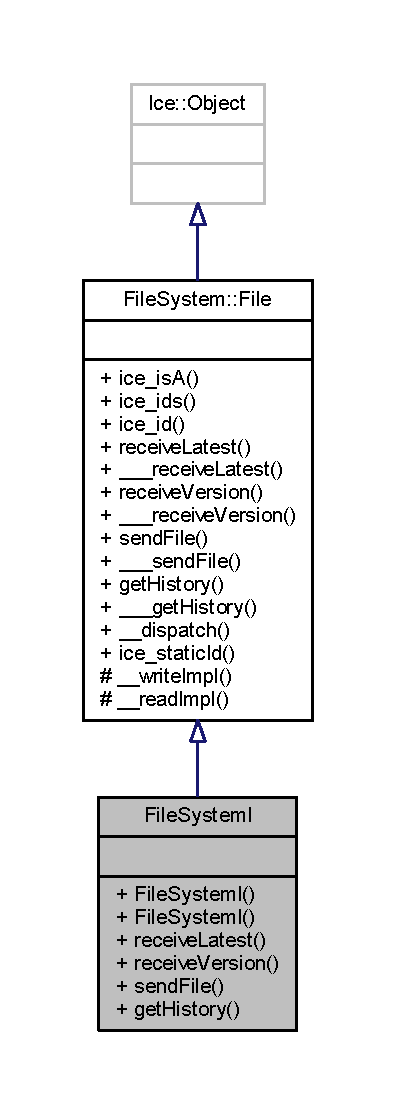
\includegraphics[width=190pt]{class_file_system_i__inherit__graph}
\end{center}
\end{figure}


Collaboration diagram for File\+System\+I\+:
\nopagebreak
\begin{figure}[H]
\begin{center}
\leavevmode
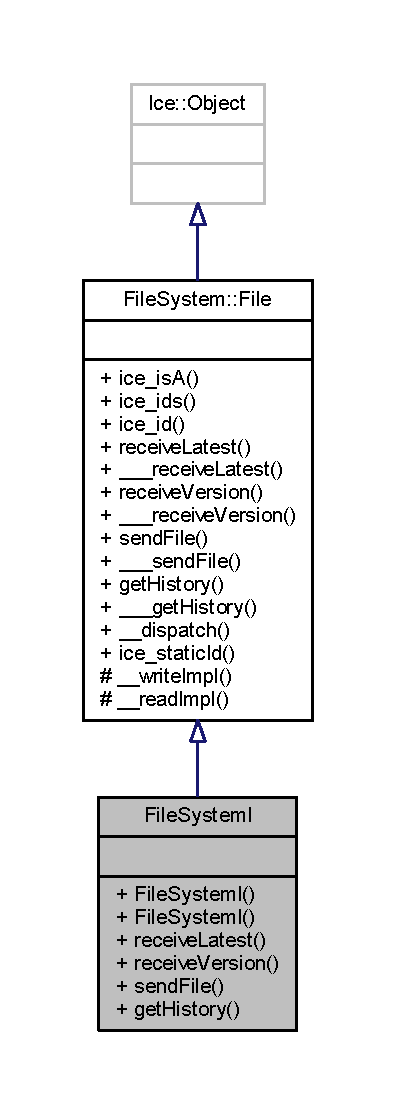
\includegraphics[width=190pt]{class_file_system_i__coll__graph}
\end{center}
\end{figure}
\subsection*{Public Member Functions}
\begin{DoxyCompactItemize}
\item 
\hyperlink{class_file_system_i_a74df9a51af59eeb364c5f570f955d82a}{File\+System\+I} (std\+::string main\+\_\+node)
\item 
\hyperlink{class_file_system_i_a9a61c34763e63d0d81183ff2ed7137f2}{File\+System\+I} ()
\item 
virtual \hyperlink{namespace_file_system_a5c85de065f9c451ae1d1dea2dacb68c5}{File\+System\+::\+Byte\+Seq} \hyperlink{class_file_system_i_abc9d41f5639080ba30ed563e579249c2}{receive\+Latest} (const std\+::string \&sec, const std\+::string \&art, const std\+::string \&type, const std\+::string \&f\+Name, const Ice\+::\+Current \&c)
\item 
virtual \hyperlink{namespace_file_system_a5c85de065f9c451ae1d1dea2dacb68c5}{File\+System\+::\+Byte\+Seq} \hyperlink{class_file_system_i_a5fa337576e6762b2b77f80b6e081b016}{receive\+Version} (const std\+::string \&sec, const std\+::string \&art, const std\+::string \&type, const std\+::string \&f\+Name, const int ver, const Ice\+::\+Current \&c)
\item 
virtual bool \hyperlink{class_file_system_i_a6f436b8f834663f35556b9e40c59df73}{send\+File} (const std\+::string \&sec, const std\+::string \&art, const std\+::string \&type, const std\+::string \&f\+Name\+Ext, const \hyperlink{namespace_file_system_a5c85de065f9c451ae1d1dea2dacb68c5}{File\+System\+::\+Byte\+Seq} \&seq, const Ice\+::\+Current \&c)
\item 
virtual \hyperlink{namespace_file_system_ac32dc1eb34c060160b52edc7c4e37d6e}{File\+System\+::\+Ver\+Seq} \hyperlink{class_file_system_i_ae61cfd5357bf5c2b380bdb87c9459dd8}{get\+History} (const std\+::string \&sec, const std\+::string \&art, const std\+::string \&type, const std\+::string \&f\+Name, const Ice\+::\+Current \&c)
\end{DoxyCompactItemize}
\subsection*{Additional Inherited Members}


\subsection{Constructor \& Destructor Documentation}
\hypertarget{class_file_system_i_a74df9a51af59eeb364c5f570f955d82a}{}\index{File\+System\+I@{File\+System\+I}!File\+System\+I@{File\+System\+I}}
\index{File\+System\+I@{File\+System\+I}!File\+System\+I@{File\+System\+I}}
\subsubsection[{File\+System\+I}]{\setlength{\rightskip}{0pt plus 5cm}File\+System\+I\+::\+File\+System\+I (
\begin{DoxyParamCaption}
\item[{std\+::string}]{main\+\_\+node}
\end{DoxyParamCaption}
)}\label{class_file_system_i_a74df9a51af59eeb364c5f570f955d82a}
\hypertarget{class_file_system_i_a9a61c34763e63d0d81183ff2ed7137f2}{}\index{File\+System\+I@{File\+System\+I}!File\+System\+I@{File\+System\+I}}
\index{File\+System\+I@{File\+System\+I}!File\+System\+I@{File\+System\+I}}
\subsubsection[{File\+System\+I}]{\setlength{\rightskip}{0pt plus 5cm}File\+System\+I\+::\+File\+System\+I (
\begin{DoxyParamCaption}
{}
\end{DoxyParamCaption}
)}\label{class_file_system_i_a9a61c34763e63d0d81183ff2ed7137f2}


\subsection{Member Function Documentation}
\hypertarget{class_file_system_i_ae61cfd5357bf5c2b380bdb87c9459dd8}{}\index{File\+System\+I@{File\+System\+I}!get\+History@{get\+History}}
\index{get\+History@{get\+History}!File\+System\+I@{File\+System\+I}}
\subsubsection[{get\+History}]{\setlength{\rightskip}{0pt plus 5cm}{\bf File\+System\+::\+Ver\+Seq} File\+System\+I\+::get\+History (
\begin{DoxyParamCaption}
\item[{const std\+::string \&}]{sec, }
\item[{const std\+::string \&}]{art, }
\item[{const std\+::string \&}]{type, }
\item[{const std\+::string \&}]{f\+Name, }
\item[{const Ice\+::\+Current \&}]{c}
\end{DoxyParamCaption}
)\hspace{0.3cm}{\ttfamily [virtual]}}\label{class_file_system_i_ae61cfd5357bf5c2b380bdb87c9459dd8}
\hypertarget{class_file_system_i_abc9d41f5639080ba30ed563e579249c2}{}\index{File\+System\+I@{File\+System\+I}!receive\+Latest@{receive\+Latest}}
\index{receive\+Latest@{receive\+Latest}!File\+System\+I@{File\+System\+I}}
\subsubsection[{receive\+Latest}]{\setlength{\rightskip}{0pt plus 5cm}{\bf File\+System\+::\+Byte\+Seq} File\+System\+I\+::receive\+Latest (
\begin{DoxyParamCaption}
\item[{const std\+::string \&}]{sec, }
\item[{const std\+::string \&}]{art, }
\item[{const std\+::string \&}]{type, }
\item[{const std\+::string \&}]{f\+Name, }
\item[{const Ice\+::\+Current \&}]{c}
\end{DoxyParamCaption}
)\hspace{0.3cm}{\ttfamily [virtual]}}\label{class_file_system_i_abc9d41f5639080ba30ed563e579249c2}
\hypertarget{class_file_system_i_a5fa337576e6762b2b77f80b6e081b016}{}\index{File\+System\+I@{File\+System\+I}!receive\+Version@{receive\+Version}}
\index{receive\+Version@{receive\+Version}!File\+System\+I@{File\+System\+I}}
\subsubsection[{receive\+Version}]{\setlength{\rightskip}{0pt plus 5cm}{\bf File\+System\+::\+Byte\+Seq} File\+System\+I\+::receive\+Version (
\begin{DoxyParamCaption}
\item[{const std\+::string \&}]{sec, }
\item[{const std\+::string \&}]{art, }
\item[{const std\+::string \&}]{type, }
\item[{const std\+::string \&}]{f\+Name, }
\item[{const int}]{ver, }
\item[{const Ice\+::\+Current \&}]{c}
\end{DoxyParamCaption}
)\hspace{0.3cm}{\ttfamily [virtual]}}\label{class_file_system_i_a5fa337576e6762b2b77f80b6e081b016}
\hypertarget{class_file_system_i_a6f436b8f834663f35556b9e40c59df73}{}\index{File\+System\+I@{File\+System\+I}!send\+File@{send\+File}}
\index{send\+File@{send\+File}!File\+System\+I@{File\+System\+I}}
\subsubsection[{send\+File}]{\setlength{\rightskip}{0pt plus 5cm}bool File\+System\+I\+::send\+File (
\begin{DoxyParamCaption}
\item[{const std\+::string \&}]{sec, }
\item[{const std\+::string \&}]{art, }
\item[{const std\+::string \&}]{type, }
\item[{const std\+::string \&}]{f\+Name\+Ext, }
\item[{const {\bf File\+System\+::\+Byte\+Seq} \&}]{seq, }
\item[{const Ice\+::\+Current \&}]{c}
\end{DoxyParamCaption}
)\hspace{0.3cm}{\ttfamily [virtual]}}\label{class_file_system_i_a6f436b8f834663f35556b9e40c59df73}


The documentation for this class was generated from the following files\+:\begin{DoxyCompactItemize}
\item 
\hyperlink{_file_system_i_8h}{File\+System\+I.\+h}\item 
\hyperlink{_file_system_i_8cpp}{File\+System\+I.\+cpp}\end{DoxyCompactItemize}

\hypertarget{class_receiver}{}\section{Receiver Class Reference}
\label{class_receiver}\index{Receiver@{Receiver}}


{\ttfamily \#include $<$Receiver.\+h$>$}



Collaboration diagram for Receiver\+:
\nopagebreak
\begin{figure}[H]
\begin{center}
\leavevmode
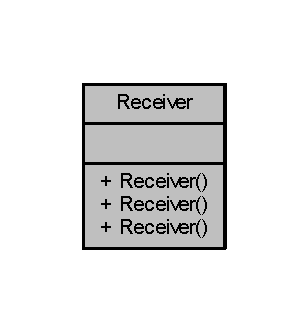
\includegraphics[width=148pt]{class_receiver__coll__graph}
\end{center}
\end{figure}
\subsection*{Public Member Functions}
\begin{DoxyCompactItemize}
\item 
\hyperlink{class_receiver_afd5190f7818573d9219ae9f41f903c7e}{Receiver} (const std\+::string path=\char`\"{}C\+:/Users/Briggs 419 Server/Dropbox/Issue\char`\"{})
\item 
\hyperlink{class_receiver_a4e5f3f9698e0f924127bf90569a524ee}{Receiver} (const int \&num, const std\+::string \&con, const std\+::string path)
\item 
\hyperlink{class_receiver_a37ff54164538c6093a6d326e7b9b1d8b}{Receiver} (const int \&num, const std\+::string path=\char`\"{}C\+:/Programs\char`\"{})
\end{DoxyCompactItemize}


\subsection{Constructor \& Destructor Documentation}
\hypertarget{class_receiver_afd5190f7818573d9219ae9f41f903c7e}{}\index{Receiver@{Receiver}!Receiver@{Receiver}}
\index{Receiver@{Receiver}!Receiver@{Receiver}}
\subsubsection[{Receiver}]{\setlength{\rightskip}{0pt plus 5cm}Receiver\+::\+Receiver (
\begin{DoxyParamCaption}
\item[{const std\+::string}]{path = {\ttfamily \char`\"{}C\+:/Users/Briggs~419~Server/Dropbox/Issue\char`\"{}}}
\end{DoxyParamCaption}
)}\label{class_receiver_afd5190f7818573d9219ae9f41f903c7e}
\hypertarget{class_receiver_a4e5f3f9698e0f924127bf90569a524ee}{}\index{Receiver@{Receiver}!Receiver@{Receiver}}
\index{Receiver@{Receiver}!Receiver@{Receiver}}
\subsubsection[{Receiver}]{\setlength{\rightskip}{0pt plus 5cm}Receiver\+::\+Receiver (
\begin{DoxyParamCaption}
\item[{const int \&}]{num, }
\item[{const std\+::string \&}]{con, }
\item[{const std\+::string}]{path}
\end{DoxyParamCaption}
)}\label{class_receiver_a4e5f3f9698e0f924127bf90569a524ee}
\hypertarget{class_receiver_a37ff54164538c6093a6d326e7b9b1d8b}{}\index{Receiver@{Receiver}!Receiver@{Receiver}}
\index{Receiver@{Receiver}!Receiver@{Receiver}}
\subsubsection[{Receiver}]{\setlength{\rightskip}{0pt plus 5cm}Receiver\+::\+Receiver (
\begin{DoxyParamCaption}
\item[{const int \&}]{num, }
\item[{const std\+::string}]{path = {\ttfamily \char`\"{}C\+:/Programs\char`\"{}}}
\end{DoxyParamCaption}
)}\label{class_receiver_a37ff54164538c6093a6d326e7b9b1d8b}


The documentation for this class was generated from the following files\+:\begin{DoxyCompactItemize}
\item 
\hyperlink{_receiver_8h}{Receiver.\+h}\item 
\hyperlink{_receiver_8cpp}{Receiver.\+cpp}\end{DoxyCompactItemize}

\hypertarget{struct_ice_1_1_streamable_traits_3_01_1_1_file_system_1_1_version_01_4}{}\section{Ice\+:\+:Streamable\+Traits$<$ \+:\+:File\+System\+:\+:Version $>$ Struct Template Reference}
\label{struct_ice_1_1_streamable_traits_3_01_1_1_file_system_1_1_version_01_4}\index{Ice\+::\+Streamable\+Traits$<$ \+::\+File\+System\+::\+Version $>$@{Ice\+::\+Streamable\+Traits$<$ \+::\+File\+System\+::\+Version $>$}}


{\ttfamily \#include $<$File\+System.\+h$>$}



Collaboration diagram for Ice\+:\+:Streamable\+Traits$<$ \+:\+:File\+System\+:\+:Version $>$\+:
\nopagebreak
\begin{figure}[H]
\begin{center}
\leavevmode
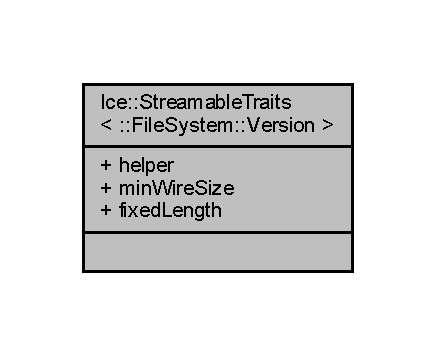
\includegraphics[width=209pt]{struct_ice_1_1_streamable_traits_3_01_1_1_file_system_1_1_version_01_4__coll__graph}
\end{center}
\end{figure}
\subsection*{Static Public Attributes}
\begin{DoxyCompactItemize}
\item 
static const Stream\+Helper\+Category \hyperlink{struct_ice_1_1_streamable_traits_3_01_1_1_file_system_1_1_version_01_4_add349dd746a44c2f0b7828e02bcbbb87}{helper} = Stream\+Helper\+Category\+Struct
\item 
static const int \hyperlink{struct_ice_1_1_streamable_traits_3_01_1_1_file_system_1_1_version_01_4_ade824a15ad09894f99e4e26e4ea59d12}{min\+Wire\+Size} = 5
\item 
static const bool \hyperlink{struct_ice_1_1_streamable_traits_3_01_1_1_file_system_1_1_version_01_4_a2aa04e83f01df92e2d2271004f71f744}{fixed\+Length} = false
\end{DoxyCompactItemize}


\subsection{Member Data Documentation}
\hypertarget{struct_ice_1_1_streamable_traits_3_01_1_1_file_system_1_1_version_01_4_a2aa04e83f01df92e2d2271004f71f744}{}\index{Ice\+::\+Streamable\+Traits$<$ \+::\+File\+System\+::\+Version $>$@{Ice\+::\+Streamable\+Traits$<$ \+::\+File\+System\+::\+Version $>$}!fixed\+Length@{fixed\+Length}}
\index{fixed\+Length@{fixed\+Length}!Ice\+::\+Streamable\+Traits$<$ \+::\+File\+System\+::\+Version $>$@{Ice\+::\+Streamable\+Traits$<$ \+::\+File\+System\+::\+Version $>$}}
\subsubsection[{fixed\+Length}]{\setlength{\rightskip}{0pt plus 5cm}const bool Ice\+::\+Streamable\+Traits$<$ \+::{\bf File\+System\+::\+Version} $>$\+::fixed\+Length = false\hspace{0.3cm}{\ttfamily [static]}}\label{struct_ice_1_1_streamable_traits_3_01_1_1_file_system_1_1_version_01_4_a2aa04e83f01df92e2d2271004f71f744}
\hypertarget{struct_ice_1_1_streamable_traits_3_01_1_1_file_system_1_1_version_01_4_add349dd746a44c2f0b7828e02bcbbb87}{}\index{Ice\+::\+Streamable\+Traits$<$ \+::\+File\+System\+::\+Version $>$@{Ice\+::\+Streamable\+Traits$<$ \+::\+File\+System\+::\+Version $>$}!helper@{helper}}
\index{helper@{helper}!Ice\+::\+Streamable\+Traits$<$ \+::\+File\+System\+::\+Version $>$@{Ice\+::\+Streamable\+Traits$<$ \+::\+File\+System\+::\+Version $>$}}
\subsubsection[{helper}]{\setlength{\rightskip}{0pt plus 5cm}const Stream\+Helper\+Category Ice\+::\+Streamable\+Traits$<$ \+::{\bf File\+System\+::\+Version} $>$\+::helper = Stream\+Helper\+Category\+Struct\hspace{0.3cm}{\ttfamily [static]}}\label{struct_ice_1_1_streamable_traits_3_01_1_1_file_system_1_1_version_01_4_add349dd746a44c2f0b7828e02bcbbb87}
\hypertarget{struct_ice_1_1_streamable_traits_3_01_1_1_file_system_1_1_version_01_4_ade824a15ad09894f99e4e26e4ea59d12}{}\index{Ice\+::\+Streamable\+Traits$<$ \+::\+File\+System\+::\+Version $>$@{Ice\+::\+Streamable\+Traits$<$ \+::\+File\+System\+::\+Version $>$}!min\+Wire\+Size@{min\+Wire\+Size}}
\index{min\+Wire\+Size@{min\+Wire\+Size}!Ice\+::\+Streamable\+Traits$<$ \+::\+File\+System\+::\+Version $>$@{Ice\+::\+Streamable\+Traits$<$ \+::\+File\+System\+::\+Version $>$}}
\subsubsection[{min\+Wire\+Size}]{\setlength{\rightskip}{0pt plus 5cm}const int Ice\+::\+Streamable\+Traits$<$ \+::{\bf File\+System\+::\+Version} $>$\+::min\+Wire\+Size = 5\hspace{0.3cm}{\ttfamily [static]}}\label{struct_ice_1_1_streamable_traits_3_01_1_1_file_system_1_1_version_01_4_ade824a15ad09894f99e4e26e4ea59d12}


The documentation for this struct was generated from the following file\+:\begin{DoxyCompactItemize}
\item 
\hyperlink{_file_system_8h}{File\+System.\+h}\end{DoxyCompactItemize}

\hypertarget{struct_ice_1_1_stream_reader_3_01_1_1_file_system_1_1_version_00_01_s_01_4}{}\section{Ice\+:\+:Stream\+Reader$<$ \+:\+:File\+System\+:\+:Version, S $>$ Struct Template Reference}
\label{struct_ice_1_1_stream_reader_3_01_1_1_file_system_1_1_version_00_01_s_01_4}\index{Ice\+::\+Stream\+Reader$<$ \+::\+File\+System\+::\+Version, S $>$@{Ice\+::\+Stream\+Reader$<$ \+::\+File\+System\+::\+Version, S $>$}}


{\ttfamily \#include $<$File\+System.\+h$>$}



Collaboration diagram for Ice\+:\+:Stream\+Reader$<$ \+:\+:File\+System\+:\+:Version, S $>$\+:
\nopagebreak
\begin{figure}[H]
\begin{center}
\leavevmode
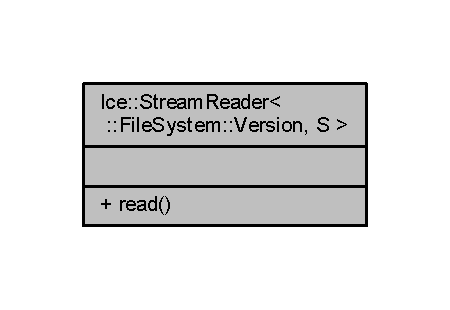
\includegraphics[width=216pt]{struct_ice_1_1_stream_reader_3_01_1_1_file_system_1_1_version_00_01_s_01_4__coll__graph}
\end{center}
\end{figure}
\subsection*{Static Public Member Functions}
\begin{DoxyCompactItemize}
\item 
static void \hyperlink{struct_ice_1_1_stream_reader_3_01_1_1_file_system_1_1_version_00_01_s_01_4_aa3e2f6ee86d7324efa51e233ef644977}{read} (S $\ast$\+\_\+\+\_\+is,\+::\hyperlink{struct_file_system_1_1_version}{File\+System\+::\+Version} \&v)
\end{DoxyCompactItemize}


\subsection{Member Function Documentation}
\hypertarget{struct_ice_1_1_stream_reader_3_01_1_1_file_system_1_1_version_00_01_s_01_4_aa3e2f6ee86d7324efa51e233ef644977}{}\index{Ice\+::\+Stream\+Reader$<$ \+::\+File\+System\+::\+Version, S $>$@{Ice\+::\+Stream\+Reader$<$ \+::\+File\+System\+::\+Version, S $>$}!read@{read}}
\index{read@{read}!Ice\+::\+Stream\+Reader$<$ \+::\+File\+System\+::\+Version, S $>$@{Ice\+::\+Stream\+Reader$<$ \+::\+File\+System\+::\+Version, S $>$}}
\subsubsection[{read}]{\setlength{\rightskip}{0pt plus 5cm}template$<$class S $>$ static void Ice\+::\+Stream\+Reader$<$ \+::{\bf File\+System\+::\+Version}, S $>$\+::read (
\begin{DoxyParamCaption}
\item[{S $\ast$}]{\+\_\+\+\_\+is, }
\item[{\+::{\bf File\+System\+::\+Version} \&}]{v}
\end{DoxyParamCaption}
)\hspace{0.3cm}{\ttfamily [inline]}, {\ttfamily [static]}}\label{struct_ice_1_1_stream_reader_3_01_1_1_file_system_1_1_version_00_01_s_01_4_aa3e2f6ee86d7324efa51e233ef644977}


The documentation for this struct was generated from the following file\+:\begin{DoxyCompactItemize}
\item 
\hyperlink{_file_system_8h}{File\+System.\+h}\end{DoxyCompactItemize}

\hypertarget{struct_ice_1_1_stream_writer_3_01_1_1_file_system_1_1_version_00_01_s_01_4}{}\section{Ice\+:\+:Stream\+Writer$<$ \+:\+:File\+System\+:\+:Version, S $>$ Struct Template Reference}
\label{struct_ice_1_1_stream_writer_3_01_1_1_file_system_1_1_version_00_01_s_01_4}\index{Ice\+::\+Stream\+Writer$<$ \+::\+File\+System\+::\+Version, S $>$@{Ice\+::\+Stream\+Writer$<$ \+::\+File\+System\+::\+Version, S $>$}}


{\ttfamily \#include $<$File\+System.\+h$>$}



Collaboration diagram for Ice\+:\+:Stream\+Writer$<$ \+:\+:File\+System\+:\+:Version, S $>$\+:
\nopagebreak
\begin{figure}[H]
\begin{center}
\leavevmode
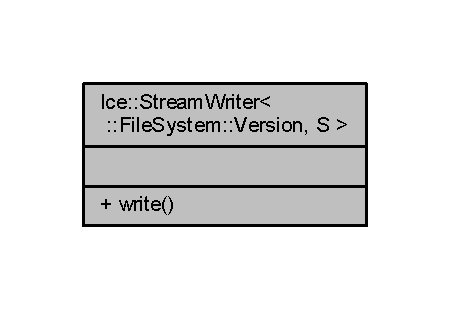
\includegraphics[width=216pt]{struct_ice_1_1_stream_writer_3_01_1_1_file_system_1_1_version_00_01_s_01_4__coll__graph}
\end{center}
\end{figure}
\subsection*{Static Public Member Functions}
\begin{DoxyCompactItemize}
\item 
static void \hyperlink{struct_ice_1_1_stream_writer_3_01_1_1_file_system_1_1_version_00_01_s_01_4_a6051f810c94db3d5d8bc00df1ac2fac5}{write} (S $\ast$\+\_\+\+\_\+os, const \+::\hyperlink{struct_file_system_1_1_version}{File\+System\+::\+Version} \&v)
\end{DoxyCompactItemize}


\subsection{Member Function Documentation}
\hypertarget{struct_ice_1_1_stream_writer_3_01_1_1_file_system_1_1_version_00_01_s_01_4_a6051f810c94db3d5d8bc00df1ac2fac5}{}\index{Ice\+::\+Stream\+Writer$<$ \+::\+File\+System\+::\+Version, S $>$@{Ice\+::\+Stream\+Writer$<$ \+::\+File\+System\+::\+Version, S $>$}!write@{write}}
\index{write@{write}!Ice\+::\+Stream\+Writer$<$ \+::\+File\+System\+::\+Version, S $>$@{Ice\+::\+Stream\+Writer$<$ \+::\+File\+System\+::\+Version, S $>$}}
\subsubsection[{write}]{\setlength{\rightskip}{0pt plus 5cm}template$<$class S $>$ static void Ice\+::\+Stream\+Writer$<$ \+::{\bf File\+System\+::\+Version}, S $>$\+::write (
\begin{DoxyParamCaption}
\item[{S $\ast$}]{\+\_\+\+\_\+os, }
\item[{const \+::{\bf File\+System\+::\+Version} \&}]{v}
\end{DoxyParamCaption}
)\hspace{0.3cm}{\ttfamily [inline]}, {\ttfamily [static]}}\label{struct_ice_1_1_stream_writer_3_01_1_1_file_system_1_1_version_00_01_s_01_4_a6051f810c94db3d5d8bc00df1ac2fac5}


The documentation for this struct was generated from the following file\+:\begin{DoxyCompactItemize}
\item 
\hyperlink{_file_system_8h}{File\+System.\+h}\end{DoxyCompactItemize}

\hypertarget{struct_file_system_1_1_version}{}\section{File\+System\+:\+:Version Struct Reference}
\label{struct_file_system_1_1_version}\index{File\+System\+::\+Version@{File\+System\+::\+Version}}


{\ttfamily \#include $<$File\+System.\+h$>$}



Collaboration diagram for File\+System\+:\+:Version\+:
\nopagebreak
\begin{figure}[H]
\begin{center}
\leavevmode
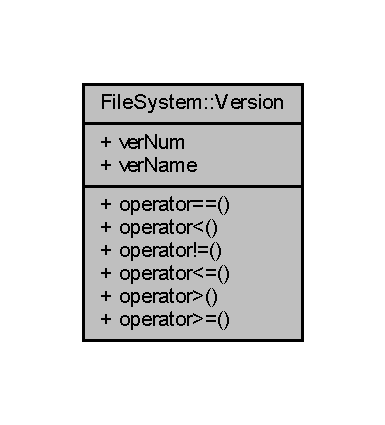
\includegraphics[width=185pt]{struct_file_system_1_1_version__coll__graph}
\end{center}
\end{figure}
\subsection*{Public Member Functions}
\begin{DoxyCompactItemize}
\item 
bool \hyperlink{struct_file_system_1_1_version_a32832303faeaffbda3e7872743a852e6}{operator==} (const \hyperlink{struct_file_system_1_1_version}{Version} \&\+\_\+\+\_\+rhs) const 
\item 
bool \hyperlink{struct_file_system_1_1_version_a9a44e56a52173f7ab4d37d4a82d72aa1}{operator$<$} (const \hyperlink{struct_file_system_1_1_version}{Version} \&\+\_\+\+\_\+rhs) const 
\item 
bool \hyperlink{struct_file_system_1_1_version_a736ea241f3c14654d6c8f4483516f2c9}{operator!=} (const \hyperlink{struct_file_system_1_1_version}{Version} \&\+\_\+\+\_\+rhs) const 
\item 
bool \hyperlink{struct_file_system_1_1_version_a09a411f27ec8c250387ad898b7d37857}{operator$<$=} (const \hyperlink{struct_file_system_1_1_version}{Version} \&\+\_\+\+\_\+rhs) const 
\item 
bool \hyperlink{struct_file_system_1_1_version_a364094d081cad8f20e76a32b7b82ebcb}{operator$>$} (const \hyperlink{struct_file_system_1_1_version}{Version} \&\+\_\+\+\_\+rhs) const 
\item 
bool \hyperlink{struct_file_system_1_1_version_a6296852fc8eac255bcc23c4f586cb6b1}{operator$>$=} (const \hyperlink{struct_file_system_1_1_version}{Version} \&\+\_\+\+\_\+rhs) const 
\end{DoxyCompactItemize}
\subsection*{Public Attributes}
\begin{DoxyCompactItemize}
\item 
\+::Ice\+::\+Int \hyperlink{struct_file_system_1_1_version_afdc710dd81f2d721b432b3baa58ec58a}{ver\+Num}
\item 
\+::std\+::string \hyperlink{struct_file_system_1_1_version_ae304c0f218e096f2d6edf7aef9f29068}{ver\+Name}
\end{DoxyCompactItemize}


\subsection{Member Function Documentation}
\hypertarget{struct_file_system_1_1_version_a736ea241f3c14654d6c8f4483516f2c9}{}\index{File\+System\+::\+Version@{File\+System\+::\+Version}!operator"!=@{operator"!=}}
\index{operator"!=@{operator"!=}!File\+System\+::\+Version@{File\+System\+::\+Version}}
\subsubsection[{operator"!=}]{\setlength{\rightskip}{0pt plus 5cm}bool File\+System\+::\+Version\+::operator!= (
\begin{DoxyParamCaption}
\item[{const {\bf Version} \&}]{\+\_\+\+\_\+rhs}
\end{DoxyParamCaption}
) const\hspace{0.3cm}{\ttfamily [inline]}}\label{struct_file_system_1_1_version_a736ea241f3c14654d6c8f4483516f2c9}
\hypertarget{struct_file_system_1_1_version_a9a44e56a52173f7ab4d37d4a82d72aa1}{}\index{File\+System\+::\+Version@{File\+System\+::\+Version}!operator$<$@{operator$<$}}
\index{operator$<$@{operator$<$}!File\+System\+::\+Version@{File\+System\+::\+Version}}
\subsubsection[{operator$<$}]{\setlength{\rightskip}{0pt plus 5cm}bool File\+System\+::\+Version\+::operator$<$ (
\begin{DoxyParamCaption}
\item[{const {\bf Version} \&}]{\+\_\+\+\_\+rhs}
\end{DoxyParamCaption}
) const\hspace{0.3cm}{\ttfamily [inline]}}\label{struct_file_system_1_1_version_a9a44e56a52173f7ab4d37d4a82d72aa1}
\hypertarget{struct_file_system_1_1_version_a09a411f27ec8c250387ad898b7d37857}{}\index{File\+System\+::\+Version@{File\+System\+::\+Version}!operator$<$=@{operator$<$=}}
\index{operator$<$=@{operator$<$=}!File\+System\+::\+Version@{File\+System\+::\+Version}}
\subsubsection[{operator$<$=}]{\setlength{\rightskip}{0pt plus 5cm}bool File\+System\+::\+Version\+::operator$<$= (
\begin{DoxyParamCaption}
\item[{const {\bf Version} \&}]{\+\_\+\+\_\+rhs}
\end{DoxyParamCaption}
) const\hspace{0.3cm}{\ttfamily [inline]}}\label{struct_file_system_1_1_version_a09a411f27ec8c250387ad898b7d37857}
\hypertarget{struct_file_system_1_1_version_a32832303faeaffbda3e7872743a852e6}{}\index{File\+System\+::\+Version@{File\+System\+::\+Version}!operator==@{operator==}}
\index{operator==@{operator==}!File\+System\+::\+Version@{File\+System\+::\+Version}}
\subsubsection[{operator==}]{\setlength{\rightskip}{0pt plus 5cm}bool File\+System\+::\+Version\+::operator== (
\begin{DoxyParamCaption}
\item[{const {\bf Version} \&}]{\+\_\+\+\_\+rhs}
\end{DoxyParamCaption}
) const\hspace{0.3cm}{\ttfamily [inline]}}\label{struct_file_system_1_1_version_a32832303faeaffbda3e7872743a852e6}
\hypertarget{struct_file_system_1_1_version_a364094d081cad8f20e76a32b7b82ebcb}{}\index{File\+System\+::\+Version@{File\+System\+::\+Version}!operator$>$@{operator$>$}}
\index{operator$>$@{operator$>$}!File\+System\+::\+Version@{File\+System\+::\+Version}}
\subsubsection[{operator$>$}]{\setlength{\rightskip}{0pt plus 5cm}bool File\+System\+::\+Version\+::operator$>$ (
\begin{DoxyParamCaption}
\item[{const {\bf Version} \&}]{\+\_\+\+\_\+rhs}
\end{DoxyParamCaption}
) const\hspace{0.3cm}{\ttfamily [inline]}}\label{struct_file_system_1_1_version_a364094d081cad8f20e76a32b7b82ebcb}
\hypertarget{struct_file_system_1_1_version_a6296852fc8eac255bcc23c4f586cb6b1}{}\index{File\+System\+::\+Version@{File\+System\+::\+Version}!operator$>$=@{operator$>$=}}
\index{operator$>$=@{operator$>$=}!File\+System\+::\+Version@{File\+System\+::\+Version}}
\subsubsection[{operator$>$=}]{\setlength{\rightskip}{0pt plus 5cm}bool File\+System\+::\+Version\+::operator$>$= (
\begin{DoxyParamCaption}
\item[{const {\bf Version} \&}]{\+\_\+\+\_\+rhs}
\end{DoxyParamCaption}
) const\hspace{0.3cm}{\ttfamily [inline]}}\label{struct_file_system_1_1_version_a6296852fc8eac255bcc23c4f586cb6b1}


\subsection{Member Data Documentation}
\hypertarget{struct_file_system_1_1_version_ae304c0f218e096f2d6edf7aef9f29068}{}\index{File\+System\+::\+Version@{File\+System\+::\+Version}!ver\+Name@{ver\+Name}}
\index{ver\+Name@{ver\+Name}!File\+System\+::\+Version@{File\+System\+::\+Version}}
\subsubsection[{ver\+Name}]{\setlength{\rightskip}{0pt plus 5cm}\+::std\+::string File\+System\+::\+Version\+::ver\+Name}\label{struct_file_system_1_1_version_ae304c0f218e096f2d6edf7aef9f29068}
\hypertarget{struct_file_system_1_1_version_afdc710dd81f2d721b432b3baa58ec58a}{}\index{File\+System\+::\+Version@{File\+System\+::\+Version}!ver\+Num@{ver\+Num}}
\index{ver\+Num@{ver\+Num}!File\+System\+::\+Version@{File\+System\+::\+Version}}
\subsubsection[{ver\+Num}]{\setlength{\rightskip}{0pt plus 5cm}\+::Ice\+::\+Int File\+System\+::\+Version\+::ver\+Num}\label{struct_file_system_1_1_version_afdc710dd81f2d721b432b3baa58ec58a}


The documentation for this struct was generated from the following file\+:\begin{DoxyCompactItemize}
\item 
\hyperlink{_file_system_8h}{File\+System.\+h}\end{DoxyCompactItemize}

\chapter{File Documentation}
\hypertarget{_file_system_8cpp}{}\section{File\+System.\+cpp File Reference}
\label{_file_system_8cpp}\index{File\+System.\+cpp@{File\+System.\+cpp}}
{\ttfamily \#include \char`\"{}File\+System.\+h\char`\"{}}\\*
{\ttfamily \#include $<$Ice/\+Local\+Exception.\+h$>$}\\*
{\ttfamily \#include $<$Ice/\+Object\+Factory.\+h$>$}\\*
{\ttfamily \#include $<$Ice/\+Basic\+Stream.\+h$>$}\\*
{\ttfamily \#include $<$Ice/\+Object.\+h$>$}\\*
{\ttfamily \#include $<$Ice\+Util/\+Iterator.\+h$>$}\\*
Include dependency graph for File\+System.\+cpp\+:
\nopagebreak
\begin{figure}[H]
\begin{center}
\leavevmode
\includegraphics[width=350pt]{_file_system_8cpp__incl}
\end{center}
\end{figure}
\subsection*{Namespaces}
\begin{DoxyCompactItemize}
\item 
 \hyperlink{namespace_ice}{Ice}
\end{DoxyCompactItemize}

\hypertarget{_file_system_8h}{}\section{File\+System.\+h File Reference}
\label{_file_system_8h}\index{File\+System.\+h@{File\+System.\+h}}
{\ttfamily \#include $<$Ice/\+Proxy\+F.\+h$>$}\\*
{\ttfamily \#include $<$Ice/\+Object\+F.\+h$>$}\\*
{\ttfamily \#include $<$Ice/\+Exception.\+h$>$}\\*
{\ttfamily \#include $<$Ice/\+Local\+Object.\+h$>$}\\*
{\ttfamily \#include $<$Ice/\+Stream\+Helpers.\+h$>$}\\*
{\ttfamily \#include $<$Ice/\+Proxy.\+h$>$}\\*
{\ttfamily \#include $<$Ice/\+Object.\+h$>$}\\*
{\ttfamily \#include $<$Ice/\+Outgoing.\+h$>$}\\*
{\ttfamily \#include $<$Ice/\+Outgoing\+Async.\+h$>$}\\*
{\ttfamily \#include $<$Ice/\+Incoming.\+h$>$}\\*
{\ttfamily \#include $<$Ice/\+Direct.\+h$>$}\\*
{\ttfamily \#include $<$Ice\+Util/\+Scoped\+Array.\+h$>$}\\*
{\ttfamily \#include $<$Ice\+Util/\+Optional.\+h$>$}\\*
{\ttfamily \#include $<$Ice/\+Stream\+F.\+h$>$}\\*
{\ttfamily \#include $<$Ice/\+Undef\+Sys\+Macros.\+h$>$}\\*
Include dependency graph for File\+System.\+h\+:
\nopagebreak
\begin{figure}[H]
\begin{center}
\leavevmode
\includegraphics[width=350pt]{_file_system_8h__incl}
\end{center}
\end{figure}
This graph shows which files directly or indirectly include this file\+:
\nopagebreak
\begin{figure}[H]
\begin{center}
\leavevmode
\includegraphics[width=350pt]{_file_system_8h__dep__incl}
\end{center}
\end{figure}
\subsection*{Classes}
\begin{DoxyCompactItemize}
\item 
struct \hyperlink{struct_file_system_1_1_version}{File\+System\+::\+Version}
\item 
struct \hyperlink{struct_ice_1_1_streamable_traits_3_01_1_1_file_system_1_1_version_01_4}{Ice\+::\+Streamable\+Traits$<$ \+::\+File\+System\+::\+Version $>$}
\item 
struct \hyperlink{struct_ice_1_1_stream_writer_3_01_1_1_file_system_1_1_version_00_01_s_01_4}{Ice\+::\+Stream\+Writer$<$ \+::\+File\+System\+::\+Version, S $>$}
\item 
struct \hyperlink{struct_ice_1_1_stream_reader_3_01_1_1_file_system_1_1_version_00_01_s_01_4}{Ice\+::\+Stream\+Reader$<$ \+::\+File\+System\+::\+Version, S $>$}
\item 
class \hyperlink{class_file_system_1_1_callback___file__receive_latest___base}{File\+System\+::\+Callback\+\_\+\+File\+\_\+receive\+Latest\+\_\+\+Base}
\item 
class \hyperlink{class_file_system_1_1_callback___file__receive_version___base}{File\+System\+::\+Callback\+\_\+\+File\+\_\+receive\+Version\+\_\+\+Base}
\item 
class \hyperlink{class_file_system_1_1_callback___file__send_file___base}{File\+System\+::\+Callback\+\_\+\+File\+\_\+send\+File\+\_\+\+Base}
\item 
class \hyperlink{class_file_system_1_1_callback___file__get_history___base}{File\+System\+::\+Callback\+\_\+\+File\+\_\+get\+History\+\_\+\+Base}
\item 
class \hyperlink{class_ice_proxy_1_1_file_system_1_1_file}{Ice\+Proxy\+::\+File\+System\+::\+File}
\item 
class \hyperlink{class_ice_delegate_1_1_file_system_1_1_file}{Ice\+Delegate\+::\+File\+System\+::\+File}
\item 
class \hyperlink{class_ice_delegate_m_1_1_file_system_1_1_file}{Ice\+Delegate\+M\+::\+File\+System\+::\+File}
\item 
class \hyperlink{class_ice_delegate_d_1_1_file_system_1_1_file}{Ice\+Delegate\+D\+::\+File\+System\+::\+File}
\item 
class \hyperlink{class_file_system_1_1_file}{File\+System\+::\+File}
\item 
class \hyperlink{class_file_system_1_1_callback_n_c___file__receive_latest}{File\+System\+::\+Callback\+N\+C\+\_\+\+File\+\_\+receive\+Latest$<$ T $>$}
\item 
class \hyperlink{class_file_system_1_1_callback___file__receive_latest}{File\+System\+::\+Callback\+\_\+\+File\+\_\+receive\+Latest$<$ T, C\+T $>$}
\item 
class \hyperlink{class_file_system_1_1_callback_n_c___file__receive_version}{File\+System\+::\+Callback\+N\+C\+\_\+\+File\+\_\+receive\+Version$<$ T $>$}
\item 
class \hyperlink{class_file_system_1_1_callback___file__receive_version}{File\+System\+::\+Callback\+\_\+\+File\+\_\+receive\+Version$<$ T, C\+T $>$}
\item 
class \hyperlink{class_file_system_1_1_callback_n_c___file__send_file}{File\+System\+::\+Callback\+N\+C\+\_\+\+File\+\_\+send\+File$<$ T $>$}
\item 
class \hyperlink{class_file_system_1_1_callback___file__send_file}{File\+System\+::\+Callback\+\_\+\+File\+\_\+send\+File$<$ T, C\+T $>$}
\item 
class \hyperlink{class_file_system_1_1_callback_n_c___file__get_history}{File\+System\+::\+Callback\+N\+C\+\_\+\+File\+\_\+get\+History$<$ T $>$}
\item 
class \hyperlink{class_file_system_1_1_callback___file__get_history}{File\+System\+::\+Callback\+\_\+\+File\+\_\+get\+History$<$ T, C\+T $>$}
\end{DoxyCompactItemize}
\subsection*{Namespaces}
\begin{DoxyCompactItemize}
\item 
 \hyperlink{namespace_ice_proxy}{Ice\+Proxy}
\item 
 \hyperlink{namespace_ice_proxy_1_1_file_system}{Ice\+Proxy\+::\+File\+System}
\item 
 \hyperlink{namespace_file_system}{File\+System}
\item 
 \hyperlink{namespace_ice}{Ice}
\item 
 \hyperlink{namespace_ice_delegate}{Ice\+Delegate}
\item 
 \hyperlink{namespace_ice_delegate_1_1_file_system}{Ice\+Delegate\+::\+File\+System}
\item 
 \hyperlink{namespace_ice_delegate_m}{Ice\+Delegate\+M}
\item 
 \hyperlink{namespace_ice_delegate_m_1_1_file_system}{Ice\+Delegate\+M\+::\+File\+System}
\item 
 \hyperlink{namespace_ice_delegate_d}{Ice\+Delegate\+D}
\item 
 \hyperlink{namespace_ice_delegate_d_1_1_file_system}{Ice\+Delegate\+D\+::\+File\+System}
\end{DoxyCompactItemize}
\subsection*{Typedefs}
\begin{DoxyCompactItemize}
\item 
typedef \+::Ice\+Internal\+::\+Handle$<$ \+::\hyperlink{class_file_system_1_1_file}{File\+System\+::\+File} $>$ \hyperlink{namespace_file_system_a322304ec4ae6dc6308f79d49662764bb}{File\+System\+::\+File\+Ptr}
\item 
typedef \+::Ice\+Internal\+::\+Proxy\+Handle$<$ \+::\hyperlink{class_ice_proxy_1_1_file_system_1_1_file}{Ice\+Proxy\+::\+File\+System\+::\+File} $>$ \hyperlink{namespace_file_system_a2cca5b42d5ab231d91dd889d4d74218c}{File\+System\+::\+File\+Prx}
\item 
typedef \+::std\+::vector$<$ \+::Ice\+::\+Byte $>$ \hyperlink{namespace_file_system_a5c85de065f9c451ae1d1dea2dacb68c5}{File\+System\+::\+Byte\+Seq}
\item 
typedef \+::std\+::vector$<$ \+::\hyperlink{struct_file_system_1_1_version}{File\+System\+::\+Version} $>$ \hyperlink{namespace_file_system_ac32dc1eb34c060160b52edc7c4e37d6e}{File\+System\+::\+Ver\+Seq}
\item 
typedef \+::Ice\+Util\+::\+Handle$<$ Callback\+\_\+\+File\+\_\+receive\+Latest\+\_\+\+Base $>$ \hyperlink{namespace_file_system_a86fe38e325e02ddd26f665f486d51837}{File\+System\+::\+Callback\+\_\+\+File\+\_\+receive\+Latest\+Ptr}
\item 
typedef \+::Ice\+Util\+::\+Handle$<$ Callback\+\_\+\+File\+\_\+receive\+Version\+\_\+\+Base $>$ \hyperlink{namespace_file_system_a9f139d463637347415d1d3dadefe9bad}{File\+System\+::\+Callback\+\_\+\+File\+\_\+receive\+Version\+Ptr}
\item 
typedef \+::Ice\+Util\+::\+Handle$<$ Callback\+\_\+\+File\+\_\+send\+File\+\_\+\+Base $>$ \hyperlink{namespace_file_system_aa10040959d9776f7f500f38a2567b56e}{File\+System\+::\+Callback\+\_\+\+File\+\_\+send\+File\+Ptr}
\item 
typedef \+::Ice\+Util\+::\+Handle$<$ Callback\+\_\+\+File\+\_\+get\+History\+\_\+\+Base $>$ \hyperlink{namespace_file_system_a9dca00d90979e9c64452fc4123feed8e}{File\+System\+::\+Callback\+\_\+\+File\+\_\+get\+History\+Ptr}
\end{DoxyCompactItemize}
\subsection*{Functions}
\begin{DoxyCompactItemize}
\item 
void \hyperlink{namespace_ice_proxy_1_1_file_system_a0b249e87c3baee8b137cf42677c53635}{Ice\+Proxy\+::\+File\+System\+::\+\_\+\+\_\+read} (\+::Ice\+Internal\+::\+Basic\+Stream $\ast$,\+::Ice\+Internal\+::\+Proxy\+Handle$<$ \+::\hyperlink{class_ice_proxy_1_1_file_system_1_1_file}{Ice\+Proxy\+::\+File\+System\+::\+File} $>$ \&)
\item 
\+::Ice\+Proxy\+::\+Ice\+::\+Object $\ast$ \hyperlink{namespace_ice_proxy_1_1_file_system_acb20dd4ca34a1045e77c7e64f5faa83a}{Ice\+Proxy\+::\+File\+System\+::up\+Cast} (\+::\hyperlink{class_ice_proxy_1_1_file_system_1_1_file}{Ice\+Proxy\+::\+File\+System\+::\+File} $\ast$)
\item 
bool \hyperlink{namespace_file_system_a73ba38c87f762f68818866f670cdece9}{File\+System\+::operator==} (const File \&, const File \&)
\item 
bool \hyperlink{namespace_file_system_ace2c44fa41a64ff7b2d5262d77563c06}{File\+System\+::operator$<$} (const File \&, const File \&)
\item 
\+::Ice\+::\+Object $\ast$ \hyperlink{namespace_file_system_a918f916e3b881056468148cf34e98734}{File\+System\+::up\+Cast} (\+::\hyperlink{class_file_system_1_1_file}{File\+System\+::\+File} $\ast$)
\item 
void \hyperlink{namespace_file_system_a51d618729b59cf8ad7823ff14af488de}{File\+System\+::\+\_\+\+\_\+patch} (File\+Ptr \&, const \+::Ice\+::\+Object\+Ptr \&)
\item 
{\footnotesize template$<$class T $>$ }\\Callback\+\_\+\+File\+\_\+receive\+Latest\+Ptr \hyperlink{namespace_file_system_a8cc04448ea3637125a33672fbd8f01db}{File\+System\+::new\+Callback\+\_\+\+File\+\_\+receive\+Latest} (const Ice\+Util\+::\+Handle$<$ T $>$ \&instance, void(T\+::$\ast$cb)(const \+::\hyperlink{namespace_file_system_a5c85de065f9c451ae1d1dea2dacb68c5}{File\+System\+::\+Byte\+Seq} \&), void(T\+::$\ast$excb)(const \+::Ice\+::\+Exception \&), void(T\+::$\ast$sentcb)(bool)=0)
\item 
{\footnotesize template$<$class T $>$ }\\Callback\+\_\+\+File\+\_\+receive\+Latest\+Ptr \hyperlink{namespace_file_system_a4fbffcbd3a07944195f823e591bb353d}{File\+System\+::new\+Callback\+\_\+\+File\+\_\+receive\+Latest} (T $\ast$instance, void(T\+::$\ast$cb)(const \+::\hyperlink{namespace_file_system_a5c85de065f9c451ae1d1dea2dacb68c5}{File\+System\+::\+Byte\+Seq} \&), void(T\+::$\ast$excb)(const \+::Ice\+::\+Exception \&), void(T\+::$\ast$sentcb)(bool)=0)
\item 
{\footnotesize template$<$class T , typename C\+T $>$ }\\Callback\+\_\+\+File\+\_\+receive\+Latest\+Ptr \hyperlink{namespace_file_system_a0046b7a52a5238cb4aec849e4ccd3f15}{File\+System\+::new\+Callback\+\_\+\+File\+\_\+receive\+Latest} (const Ice\+Util\+::\+Handle$<$ T $>$ \&instance, void(T\+::$\ast$cb)(const \+::\hyperlink{namespace_file_system_a5c85de065f9c451ae1d1dea2dacb68c5}{File\+System\+::\+Byte\+Seq} \&, const C\+T \&), void(T\+::$\ast$excb)(const \+::Ice\+::\+Exception \&, const C\+T \&), void(T\+::$\ast$sentcb)(bool, const C\+T \&)=0)
\item 
{\footnotesize template$<$class T , typename C\+T $>$ }\\Callback\+\_\+\+File\+\_\+receive\+Latest\+Ptr \hyperlink{namespace_file_system_ab3edd75e3503f455de67f53659888e54}{File\+System\+::new\+Callback\+\_\+\+File\+\_\+receive\+Latest} (T $\ast$instance, void(T\+::$\ast$cb)(const \+::\hyperlink{namespace_file_system_a5c85de065f9c451ae1d1dea2dacb68c5}{File\+System\+::\+Byte\+Seq} \&, const C\+T \&), void(T\+::$\ast$excb)(const \+::Ice\+::\+Exception \&, const C\+T \&), void(T\+::$\ast$sentcb)(bool, const C\+T \&)=0)
\item 
{\footnotesize template$<$class T $>$ }\\Callback\+\_\+\+File\+\_\+receive\+Version\+Ptr \hyperlink{namespace_file_system_a42d5739a2f8c21dd11147976f3899b6a}{File\+System\+::new\+Callback\+\_\+\+File\+\_\+receive\+Version} (const Ice\+Util\+::\+Handle$<$ T $>$ \&instance, void(T\+::$\ast$cb)(const \+::\hyperlink{namespace_file_system_a5c85de065f9c451ae1d1dea2dacb68c5}{File\+System\+::\+Byte\+Seq} \&), void(T\+::$\ast$excb)(const \+::Ice\+::\+Exception \&), void(T\+::$\ast$sentcb)(bool)=0)
\item 
{\footnotesize template$<$class T $>$ }\\Callback\+\_\+\+File\+\_\+receive\+Version\+Ptr \hyperlink{namespace_file_system_a03da11fc8fef703e71e714806a453d0f}{File\+System\+::new\+Callback\+\_\+\+File\+\_\+receive\+Version} (T $\ast$instance, void(T\+::$\ast$cb)(const \+::\hyperlink{namespace_file_system_a5c85de065f9c451ae1d1dea2dacb68c5}{File\+System\+::\+Byte\+Seq} \&), void(T\+::$\ast$excb)(const \+::Ice\+::\+Exception \&), void(T\+::$\ast$sentcb)(bool)=0)
\item 
{\footnotesize template$<$class T , typename C\+T $>$ }\\Callback\+\_\+\+File\+\_\+receive\+Version\+Ptr \hyperlink{namespace_file_system_aca4582991eb93cb8a1826c2387679604}{File\+System\+::new\+Callback\+\_\+\+File\+\_\+receive\+Version} (const Ice\+Util\+::\+Handle$<$ T $>$ \&instance, void(T\+::$\ast$cb)(const \+::\hyperlink{namespace_file_system_a5c85de065f9c451ae1d1dea2dacb68c5}{File\+System\+::\+Byte\+Seq} \&, const C\+T \&), void(T\+::$\ast$excb)(const \+::Ice\+::\+Exception \&, const C\+T \&), void(T\+::$\ast$sentcb)(bool, const C\+T \&)=0)
\item 
{\footnotesize template$<$class T , typename C\+T $>$ }\\Callback\+\_\+\+File\+\_\+receive\+Version\+Ptr \hyperlink{namespace_file_system_adf4cdf405caaf42582f7d55bf48d5702}{File\+System\+::new\+Callback\+\_\+\+File\+\_\+receive\+Version} (T $\ast$instance, void(T\+::$\ast$cb)(const \+::\hyperlink{namespace_file_system_a5c85de065f9c451ae1d1dea2dacb68c5}{File\+System\+::\+Byte\+Seq} \&, const C\+T \&), void(T\+::$\ast$excb)(const \+::Ice\+::\+Exception \&, const C\+T \&), void(T\+::$\ast$sentcb)(bool, const C\+T \&)=0)
\item 
{\footnotesize template$<$class T $>$ }\\Callback\+\_\+\+File\+\_\+send\+File\+Ptr \hyperlink{namespace_file_system_a19a234cedd70c1fd80bb5f5c842c3041}{File\+System\+::new\+Callback\+\_\+\+File\+\_\+send\+File} (const Ice\+Util\+::\+Handle$<$ T $>$ \&instance, void(T\+::$\ast$cb)(bool), void(T\+::$\ast$excb)(const \+::Ice\+::\+Exception \&), void(T\+::$\ast$sentcb)(bool)=0)
\item 
{\footnotesize template$<$class T $>$ }\\Callback\+\_\+\+File\+\_\+send\+File\+Ptr \hyperlink{namespace_file_system_a940c86675dd438dacf7618250756a3c0}{File\+System\+::new\+Callback\+\_\+\+File\+\_\+send\+File} (T $\ast$instance, void(T\+::$\ast$cb)(bool), void(T\+::$\ast$excb)(const \+::Ice\+::\+Exception \&), void(T\+::$\ast$sentcb)(bool)=0)
\item 
{\footnotesize template$<$class T , typename C\+T $>$ }\\Callback\+\_\+\+File\+\_\+send\+File\+Ptr \hyperlink{namespace_file_system_a018b94a8e4bb414a2eb5b880dfd2309d}{File\+System\+::new\+Callback\+\_\+\+File\+\_\+send\+File} (const Ice\+Util\+::\+Handle$<$ T $>$ \&instance, void(T\+::$\ast$cb)(bool, const C\+T \&), void(T\+::$\ast$excb)(const \+::Ice\+::\+Exception \&, const C\+T \&), void(T\+::$\ast$sentcb)(bool, const C\+T \&)=0)
\item 
{\footnotesize template$<$class T , typename C\+T $>$ }\\Callback\+\_\+\+File\+\_\+send\+File\+Ptr \hyperlink{namespace_file_system_a617605b6d0e9224ad5d7d424600651da}{File\+System\+::new\+Callback\+\_\+\+File\+\_\+send\+File} (T $\ast$instance, void(T\+::$\ast$cb)(bool, const C\+T \&), void(T\+::$\ast$excb)(const \+::Ice\+::\+Exception \&, const C\+T \&), void(T\+::$\ast$sentcb)(bool, const C\+T \&)=0)
\item 
{\footnotesize template$<$class T $>$ }\\Callback\+\_\+\+File\+\_\+get\+History\+Ptr \hyperlink{namespace_file_system_a9c85bcf49db4963463099447f95e0dab}{File\+System\+::new\+Callback\+\_\+\+File\+\_\+get\+History} (const Ice\+Util\+::\+Handle$<$ T $>$ \&instance, void(T\+::$\ast$cb)(const \+::\hyperlink{namespace_file_system_ac32dc1eb34c060160b52edc7c4e37d6e}{File\+System\+::\+Ver\+Seq} \&), void(T\+::$\ast$excb)(const \+::Ice\+::\+Exception \&), void(T\+::$\ast$sentcb)(bool)=0)
\item 
{\footnotesize template$<$class T $>$ }\\Callback\+\_\+\+File\+\_\+get\+History\+Ptr \hyperlink{namespace_file_system_ad5d2a7211c35dfd59a100b8672b42fae}{File\+System\+::new\+Callback\+\_\+\+File\+\_\+get\+History} (T $\ast$instance, void(T\+::$\ast$cb)(const \+::\hyperlink{namespace_file_system_ac32dc1eb34c060160b52edc7c4e37d6e}{File\+System\+::\+Ver\+Seq} \&), void(T\+::$\ast$excb)(const \+::Ice\+::\+Exception \&), void(T\+::$\ast$sentcb)(bool)=0)
\item 
{\footnotesize template$<$class T , typename C\+T $>$ }\\Callback\+\_\+\+File\+\_\+get\+History\+Ptr \hyperlink{namespace_file_system_a452d710fbcda80656c790b9c5fd63518}{File\+System\+::new\+Callback\+\_\+\+File\+\_\+get\+History} (const Ice\+Util\+::\+Handle$<$ T $>$ \&instance, void(T\+::$\ast$cb)(const \+::\hyperlink{namespace_file_system_ac32dc1eb34c060160b52edc7c4e37d6e}{File\+System\+::\+Ver\+Seq} \&, const C\+T \&), void(T\+::$\ast$excb)(const \+::Ice\+::\+Exception \&, const C\+T \&), void(T\+::$\ast$sentcb)(bool, const C\+T \&)=0)
\item 
{\footnotesize template$<$class T , typename C\+T $>$ }\\Callback\+\_\+\+File\+\_\+get\+History\+Ptr \hyperlink{namespace_file_system_acaebd2ccc7b6507ce9791aa62af99829}{File\+System\+::new\+Callback\+\_\+\+File\+\_\+get\+History} (T $\ast$instance, void(T\+::$\ast$cb)(const \+::\hyperlink{namespace_file_system_ac32dc1eb34c060160b52edc7c4e37d6e}{File\+System\+::\+Ver\+Seq} \&, const C\+T \&), void(T\+::$\ast$excb)(const \+::Ice\+::\+Exception \&, const C\+T \&), void(T\+::$\ast$sentcb)(bool, const C\+T \&)=0)
\end{DoxyCompactItemize}

\hypertarget{_file_system_i_8cpp}{}\section{File\+System\+I.\+cpp File Reference}
\label{_file_system_i_8cpp}\index{File\+System\+I.\+cpp@{File\+System\+I.\+cpp}}
{\ttfamily \#include \char`\"{}File\+System\+I.\+h\char`\"{}}\\*
{\ttfamily \#include $<$fstream$>$}\\*
{\ttfamily \#include $<$Windows.\+h$>$}\\*
{\ttfamily \#include $<$string.\+h$>$}\\*
{\ttfamily \#include $<$direct.\+h$>$}\\*
{\ttfamily \#include $<$cctype$>$}\\*
Include dependency graph for File\+System\+I.\+cpp\+:
\nopagebreak
\begin{figure}[H]
\begin{center}
\leavevmode
\includegraphics[width=350pt]{_file_system_i_8cpp__incl}
\end{center}
\end{figure}

\hypertarget{_file_system_i_8h}{}\section{File\+System\+I.\+h File Reference}
\label{_file_system_i_8h}\index{File\+System\+I.\+h@{File\+System\+I.\+h}}
{\ttfamily \#include $<$Ice/\+Ice.\+h$>$}\\*
{\ttfamily \#include \char`\"{}File\+System.\+h\char`\"{}}\\*
Include dependency graph for File\+System\+I.\+h\+:
\nopagebreak
\begin{figure}[H]
\begin{center}
\leavevmode
\includegraphics[width=350pt]{_file_system_i_8h__incl}
\end{center}
\end{figure}
This graph shows which files directly or indirectly include this file\+:
\nopagebreak
\begin{figure}[H]
\begin{center}
\leavevmode
\includegraphics[width=258pt]{_file_system_i_8h__dep__incl}
\end{center}
\end{figure}
\subsection*{Classes}
\begin{DoxyCompactItemize}
\item 
class \hyperlink{class_file_system_i}{File\+System\+I}
\end{DoxyCompactItemize}

\hypertarget{main_8cpp}{}\section{main.\+cpp File Reference}
\label{main_8cpp}\index{main.\+cpp@{main.\+cpp}}
{\ttfamily \#include \char`\"{}registrationwindow.\+h\char`\"{}}\\*
{\ttfamily \#include $<$Q\+Application$>$}\\*
{\ttfamily \#include \char`\"{}client.\+h\char`\"{}}\\*
{\ttfamily \#include $<$iostream$>$}\\*
{\ttfamily \#include \char`\"{}loginwindow.\+h\char`\"{}}\\*
{\ttfamily \#include $<$qmessagebox.\+h$>$}\\*
{\ttfamily \#include \char`\"{}alert.\+h\char`\"{}}\\*
{\ttfamily \#include \char`\"{}mainwindow.\+h\char`\"{}}\\*
{\ttfamily \#include \char`\"{}Sender.\+h\char`\"{}}\\*
{\ttfamily \#include \char`\"{}newarticleworkspacewindow.\+h\char`\"{}}\\*
Include dependency graph for main.\+cpp\+:
\nopagebreak
\begin{figure}[H]
\begin{center}
\leavevmode
\includegraphics[width=350pt]{main_8cpp__incl}
\end{center}
\end{figure}
\subsection*{Functions}
\begin{DoxyCompactItemize}
\item 
int \hyperlink{main_8cpp_a0ddf1224851353fc92bfbff6f499fa97}{main} (int argc, char $\ast$argv\mbox{[}$\,$\mbox{]})
\end{DoxyCompactItemize}


\subsection{Function Documentation}
\hypertarget{main_8cpp_a0ddf1224851353fc92bfbff6f499fa97}{}\index{main.\+cpp@{main.\+cpp}!main@{main}}
\index{main@{main}!main.\+cpp@{main.\+cpp}}
\subsubsection[{main}]{\setlength{\rightskip}{0pt plus 5cm}int main (
\begin{DoxyParamCaption}
\item[{int}]{argc, }
\item[{char $\ast$}]{argv\mbox{[}$\,$\mbox{]}}
\end{DoxyParamCaption}
)}\label{main_8cpp_a0ddf1224851353fc92bfbff6f499fa97}


Here is the call graph for this function\+:
\nopagebreak
\begin{figure}[H]
\begin{center}
\leavevmode
\includegraphics[width=350pt]{main_8cpp_a0ddf1224851353fc92bfbff6f499fa97_cgraph}
\end{center}
\end{figure}



\hypertarget{_receiver_8cpp}{}\section{Receiver.\+cpp File Reference}
\label{_receiver_8cpp}\index{Receiver.\+cpp@{Receiver.\+cpp}}
{\ttfamily \#include \char`\"{}Receiver.\+h\char`\"{}}\\*
{\ttfamily \#include \char`\"{}File\+System.\+h\char`\"{}}\\*
{\ttfamily \#include \char`\"{}File\+System\+I.\+h\char`\"{}}\\*
Include dependency graph for Receiver.\+cpp\+:
\nopagebreak
\begin{figure}[H]
\begin{center}
\leavevmode
\includegraphics[width=350pt]{_receiver_8cpp__incl}
\end{center}
\end{figure}

\hypertarget{_receiver_8h}{}\section{Receiver.\+h File Reference}
\label{_receiver_8h}\index{Receiver.\+h@{Receiver.\+h}}
{\ttfamily \#include $<$Ice/\+Ice.\+h$>$}\\*
{\ttfamily \#include \char`\"{}File\+System.\+h\char`\"{}}\\*
{\ttfamily \#include $<$fstream$>$}\\*
{\ttfamily \#include $<$string$>$}\\*
Include dependency graph for Receiver.\+h\+:
\nopagebreak
\begin{figure}[H]
\begin{center}
\leavevmode
\includegraphics[width=350pt]{_receiver_8h__incl}
\end{center}
\end{figure}
This graph shows which files directly or indirectly include this file\+:
\nopagebreak
\begin{figure}[H]
\begin{center}
\leavevmode
\includegraphics[width=226pt]{_receiver_8h__dep__incl}
\end{center}
\end{figure}
\subsection*{Classes}
\begin{DoxyCompactItemize}
\item 
class \hyperlink{class_receiver}{Receiver}
\end{DoxyCompactItemize}

%--- End generated contents ---

% Index
\backmatter
\newpage
\phantomsection
\clearemptydoublepage
\addcontentsline{toc}{chapter}{Index}
\printindex

\end{document}
